% \documentclass[conference,compsoc]{IEEEtran}
%DIF LATEXDIFF DIFFERENCE FILE
%DIF DEL ../paper-android-malware-main/main.tex   Mon Jan  5 12:30:58 2026
%DIF ADD ./main.tex                               Tue Jan  6 15:00:28 2026
\documentclass[manuscript,screen,review]{acmart}
\usepackage{shortcuts}

% to be able to draw some self-contained figs
\usepackage{tikz}
\usepackage{amsmath}
\usepackage{xspace}
\usepackage{subcaption}	
\usepackage{enumitem}
\usepackage{booktabs}
\usepackage{adjustbox}	
\usepackage{graphicx}	
\usepackage{multirow}	
\usepackage{hyperref}
\usepackage{balance}
\usepackage{stfloats}
\usepackage[utf8]{inputenc}
\usepackage{threeparttable}
\usepackage{framed}
\usepackage{listings}
\usepackage{microtype}
\usepackage{diagbox}
\usepackage{url}
\usepackage{makecell}
\usepackage{threeparttable}
\usepackage{color}
\usepackage{xcolor}
\usepackage{colortbl}
\usepackage{mathtools}
\usepackage{nccmath}
% \let\Bbbk\relax 
% \usepackage{amssymb}
\usepackage{algorithm}
\usepackage{algorithmic}
% \usepackage{cite}

% \hyphenation{op-tical net-works semi-conduc-tor IEEE-Xplore}

\usepackage{wasysym}
\newcommand{\ymark}{\CIRCLE}
\newcommand{\nmark}{\Circle}
\newcommand{\halfmark}{\LEFTcircle}

\usepackage{pifont}
\newcommand{\cmark}{\ding{52}} %52
\newcommand{\xmark}{\ding{56}} %56

\usepackage{tcolorbox}
\newtcolorbox{conclusionbox}{colback=gray!8,colframe=black,width=\linewidth,arc=0.6mm, boxrule=0.4pt, left=1mm,right=1mm,top=0.5mm,bottom=0.5mm,before skip=2mm,after skip=0mm}


\definecolor{patriarch}{rgb}{0.5, 0.0, 0.5}
\definecolor{acmblue}{cmyk}{1, 0.1, 0, 0.1}
\definecolor{acmdarkblue}{cmyk}{1, 0.2, 0, 0.15}
\hypersetup{
  colorlinks,
  citecolor=patriarch,
  linkcolor=patriarch,
  urlcolor=acmdarkblue
}

% To refine the paper, I have made a brief to-do list as follows:
% 1) Clarify the usage of our framework, especially how to use it to implement and compare new malware detectors.
% 2) Provide a detailed discussion on how these 12 approaches were selected.
% 3) Emphasize our goal to revisit the status of existing Android malware detectors and highlight our contributions.
% 4) Address the reviewers’ concerns about not including data from 2021 to 2023. I found that the size of malware distributed in 2021 to 2023 in AndroZoo is not enough. I will clarify this in the dataset section.
% 5) Discuss the potential use of LLM in Android analysis, specifically whether it could help address some of the challenges we have identified.
\setcopyright{none}

\settopmatter{printacmref=false}

\makeatletter
\renewcommand\@copyrightpermission{}
\makeatother
% --------------
% \copyrightyear{2018}
% \acmYear{2018}
% \acmDOI{XXXXXXX.XXXXXXX}
% %% These commands are for a PROCEEDINGS abstract or paper.
% \acmConference[Conference acronym 'XX]{Make sure to enter the correct
%   conference title from your rights confirmation email}{June 03--05,
%   2018}{Woodstock, NY}
%
%  Uncomment \acmBooktitle if the title of the proceedings is different
%  from ``Proceedings of ...''!
%
%\acmBooktitle{Woodstock '18: ACM Symposium on Neural Gaze Detection,
%  June 03--05, 2018, Woodstock, NY}
% \acmISBN{978-1-4503-XXXX-X/2018/06}
%DIF PREAMBLE EXTENSION ADDED BY LATEXDIFF
%DIF UNDERLINE PREAMBLE %DIF PREAMBLE
\RequirePackage[normalem]{ulem} %DIF PREAMBLE
\RequirePackage{color}\definecolor{RED}{rgb}{1,0,0}\definecolor{BLUE}{rgb}{0,0,1} %DIF PREAMBLE
\providecommand{\DIFaddtex}[1]{{\protect\color{blue}\uwave{#1}}} %DIF PREAMBLE
\providecommand{\DIFdeltex}[1]{{\protect\color{red}\sout{#1}}} %DIF PREAMBLE
%DIF SAFE PREAMBLE %DIF PREAMBLE
\providecommand{\DIFaddbegin}{} %DIF PREAMBLE
\providecommand{\DIFaddend}{} %DIF PREAMBLE
\providecommand{\DIFdelbegin}{} %DIF PREAMBLE
\providecommand{\DIFdelend}{} %DIF PREAMBLE
\providecommand{\DIFmodbegin}{} %DIF PREAMBLE
\providecommand{\DIFmodend}{} %DIF PREAMBLE
%DIF FLOATSAFE PREAMBLE %DIF PREAMBLE
\providecommand{\DIFaddFL}[1]{\DIFadd{#1}} %DIF PREAMBLE
\providecommand{\DIFdelFL}[1]{\DIFdel{#1}} %DIF PREAMBLE
\providecommand{\DIFaddbeginFL}{} %DIF PREAMBLE
\providecommand{\DIFaddendFL}{} %DIF PREAMBLE
\providecommand{\DIFdelbeginFL}{} %DIF PREAMBLE
\providecommand{\DIFdelendFL}{} %DIF PREAMBLE
%DIF HYPERREF PREAMBLE %DIF PREAMBLE
\providecommand{\DIFadd}[1]{\texorpdfstring{\DIFaddtex{#1}}{#1}} %DIF PREAMBLE
\providecommand{\DIFdel}[1]{\texorpdfstring{\DIFdeltex{#1}}{}} %DIF PREAMBLE
\newcommand{\DIFscaledelfig}{0.5}
%DIF HIGHLIGHTGRAPHICS PREAMBLE %DIF PREAMBLE
\RequirePackage{settobox} %DIF PREAMBLE
\RequirePackage{letltxmacro} %DIF PREAMBLE
\newsavebox{\DIFdelgraphicsbox} %DIF PREAMBLE
\newlength{\DIFdelgraphicswidth} %DIF PREAMBLE
\newlength{\DIFdelgraphicsheight} %DIF PREAMBLE
% store original definition of \includegraphics %DIF PREAMBLE
\LetLtxMacro{\DIFOincludegraphics}{\includegraphics} %DIF PREAMBLE
\newcommand{\DIFaddincludegraphics}[2][]{{\color{blue}\fbox{\DIFOincludegraphics[#1]{#2}}}} %DIF PREAMBLE
\newcommand{\DIFdelincludegraphics}[2][]{% %DIF PREAMBLE
\sbox{\DIFdelgraphicsbox}{\DIFOincludegraphics[#1]{#2}}% %DIF PREAMBLE
\settoboxwidth{\DIFdelgraphicswidth}{\DIFdelgraphicsbox} %DIF PREAMBLE
\settoboxtotalheight{\DIFdelgraphicsheight}{\DIFdelgraphicsbox} %DIF PREAMBLE
\scalebox{\DIFscaledelfig}{% %DIF PREAMBLE
\parbox[b]{\DIFdelgraphicswidth}{\usebox{\DIFdelgraphicsbox}\\[-\baselineskip] \rule{\DIFdelgraphicswidth}{0em}}\llap{\resizebox{\DIFdelgraphicswidth}{\DIFdelgraphicsheight}{% %DIF PREAMBLE
\setlength{\unitlength}{\DIFdelgraphicswidth}% %DIF PREAMBLE
\begin{picture}(1,1)% %DIF PREAMBLE
\thicklines\linethickness{2pt} %DIF PREAMBLE
{\color[rgb]{1,0,0}\put(0,0){\framebox(1,1){}}}% %DIF PREAMBLE
{\color[rgb]{1,0,0}\put(0,0){\line( 1,1){1}}}% %DIF PREAMBLE
{\color[rgb]{1,0,0}\put(0,1){\line(1,-1){1}}}% %DIF PREAMBLE
\end{picture}% %DIF PREAMBLE
}\hspace*{3pt}}} %DIF PREAMBLE
} %DIF PREAMBLE
\LetLtxMacro{\DIFOaddbegin}{\DIFaddbegin} %DIF PREAMBLE
\LetLtxMacro{\DIFOaddend}{\DIFaddend} %DIF PREAMBLE
\LetLtxMacro{\DIFOdelbegin}{\DIFdelbegin} %DIF PREAMBLE
\LetLtxMacro{\DIFOdelend}{\DIFdelend} %DIF PREAMBLE
\DeclareRobustCommand{\DIFaddbegin}{\DIFOaddbegin \let\includegraphics\DIFaddincludegraphics} %DIF PREAMBLE
\DeclareRobustCommand{\DIFaddend}{\DIFOaddend \let\includegraphics\DIFOincludegraphics} %DIF PREAMBLE
\DeclareRobustCommand{\DIFdelbegin}{\DIFOdelbegin \let\includegraphics\DIFdelincludegraphics} %DIF PREAMBLE
\DeclareRobustCommand{\DIFdelend}{\DIFOaddend \let\includegraphics\DIFOincludegraphics} %DIF PREAMBLE
\LetLtxMacro{\DIFOaddbeginFL}{\DIFaddbeginFL} %DIF PREAMBLE
\LetLtxMacro{\DIFOaddendFL}{\DIFaddendFL} %DIF PREAMBLE
\LetLtxMacro{\DIFOdelbeginFL}{\DIFdelbeginFL} %DIF PREAMBLE
\LetLtxMacro{\DIFOdelendFL}{\DIFdelendFL} %DIF PREAMBLE
\DeclareRobustCommand{\DIFaddbeginFL}{\DIFOaddbeginFL \let\includegraphics\DIFaddincludegraphics} %DIF PREAMBLE
\DeclareRobustCommand{\DIFaddendFL}{\DIFOaddendFL \let\includegraphics\DIFOincludegraphics} %DIF PREAMBLE
\DeclareRobustCommand{\DIFdelbeginFL}{\DIFOdelbeginFL \let\includegraphics\DIFdelincludegraphics} %DIF PREAMBLE
\DeclareRobustCommand{\DIFdelendFL}{\DIFOaddendFL \let\includegraphics\DIFOincludegraphics} %DIF PREAMBLE
%DIF AMSMATHULEM PREAMBLE %DIF PREAMBLE
\makeatletter %DIF PREAMBLE
\let\sout@orig\sout %DIF PREAMBLE
\renewcommand{\sout}[1]{\ifmmode\text{\sout@orig{\ensuremath{#1}}}\else\sout@orig{#1}\fi} %DIF PREAMBLE
\makeatother %DIF PREAMBLE
%DIF COLORLISTINGS PREAMBLE %DIF PREAMBLE
\RequirePackage{listings} %DIF PREAMBLE
\RequirePackage{color} %DIF PREAMBLE
\lstdefinelanguage{DIFcode}{ %DIF PREAMBLE
%DIF DIFCODE_UNDERLINE %DIF PREAMBLE
  moredelim=[il][\color{red}\sout]{\%DIF\ <\ }, %DIF PREAMBLE
  moredelim=[il][\color{blue}\uwave]{\%DIF\ >\ } %DIF PREAMBLE
} %DIF PREAMBLE
\lstdefinestyle{DIFverbatimstyle}{ %DIF PREAMBLE
	language=DIFcode, %DIF PREAMBLE
	basicstyle=\ttfamily, %DIF PREAMBLE
	columns=fullflexible, %DIF PREAMBLE
	keepspaces=true %DIF PREAMBLE
} %DIF PREAMBLE
\lstnewenvironment{DIFverbatim}{\lstset{style=DIFverbatimstyle}}{} %DIF PREAMBLE
\lstnewenvironment{DIFverbatim*}{\lstset{style=DIFverbatimstyle,showspaces=true}}{} %DIF PREAMBLE
\lstset{extendedchars=\true,inputencoding=utf8}

%DIF END PREAMBLE EXTENSION ADDED BY LATEXDIFF

\begin{document}

\title{Unraveling the Key of Machine Learning-based Android Malware Detection}


\author{Jiahao Liu}
\affiliation{%
  \institution{National University of Singapore}
  \city{Singapore}
  \country{Singapore}}
\email{jiahao99@comp.nus.edu.sg}
\author{Jun Zeng}
\affiliation{%
  \institution{National University of Singapore}
  \city{Singapore}
  \country{Singapore}}
\email{junzeng@comp.nus.edu.sg}
\author{Fabio Pierazzi}
\affiliation{
  \institution{University College London}
  \city{London}
  \country{United Kingdom}}
\email{f.pierazzi@ucl.ac.uk}
\author{Ziqi Yang}
\affiliation{%
  \institution{The State Key Laboratory of Blockchain and Data Security, Zhejiang University}
  \city{Hangzhou}
  \country{China}}
\affiliation{
  \institution{Hangzhou High-Tech Zone (Binjiang) Institute of Blockchain and Data Security}
  \city{Hangzhou}
  \country{China}}
\email{yangziqi@zju.edu.cn}
\author{Lorenzo Cavallaro}
\affiliation{
  \institution{University College London}
  \city{London}
  \country{United Kingdom}}
\email{l.cavallaro@ucl.ac.uk}
\author{Zhenkai Liang}
\affiliation{%
  \institution{National University of Singapore}
  \city{Singapore}
  \country{Singapore}}
\email{liangzk@comp.nus.edu.sg}

\clearpage
\thispagestyle{empty}
% --- Response Letter Page ---
\begingroup
\pagestyle{empty}
\begin{center}
  {\LARGE \textbf{Revision Response Letter}}
\end{center}
\vspace{2ex}

We appreciate the valuable feedback from the reviewers and have made improvements to the paper accordingly.
In this revision, we conducted new experiments to address the reviewers' concerns, clarified several sections, and refined the writing throughout the paper.
Below we provide a point-by-point response to the reviewers' comments.

\section*{Associate Editor}
Thanks for the overall comments and suggestions.
Here, we summarize how we address the high-level concerns raised. And in the following sections, we provide detailed responses to each reviewer's comments.

\vspace{0.1cm}
\noindent \textbf{1. Limitation of the application dataset.}

To address concerns regarding the dataset, we have expanded the discussion of its representativeness and potential limitations in Section~\ref{sec:discussion} (Dataset consideration). In addition, we collected a new dataset spanning 2021-2024 and conducted additional experiments to evaluate detector effectiveness on more recent applications. We also added stability experiments in Section~\ref{robustness} (Detector stability on different time period datasets) to demonstrate the robustness of the evaluated detectors across datasets from different time periods.

Based on these revisions, we justify that our key findings continue to hold for recent apps and reliably reflect general trends in ML-based Android malware detection.

\vspace{0.1cm}
\noindent \textbf{2. Lack of practical efficiency evaluation.}

We have expanded the efficiency evaluation in Section~\ref{efficiency} to cover the entire ML-based Android malware detection pipeline, including feature extraction, feature transformation, model training, and model prediction. In addition, we introduce new metrics --- such as memory consumption during feature extraction --- to provide a more comprehensive assessment of computational overhead. With these additions, we present a more holistic view of the computational costs associated with ML-based Android malware detection.

\vspace{0.1cm}
\noindent \textbf{3. Clarification of contributions and findings.}

We have revised the introduction in Section~\ref{sec:intro} to explicitly highlight the lack of a comprehensive investigation and a standardized framework in the field of ML-based Android malware detection. In addition, we provide a more explicit comparison with existing studies at the beginning of Section~\ref{sec:systematic_investigation}, discussing how prior work is either largely theoretical or limited in experimental scope and scalability, and falls short of offering a framework that supports flexible and reproducible evaluation and new detector development.

Our work addresses these gaps by conducting a systematic and empirical investigation of ML-based Android malware detection and by providing a general-purpose benchmarking framework to support reproducible evaluation and future research. Furthermore, we summarize our key findings and present actionable recommendations, offering clear takeaways for both researchers and practitioners.

\vspace{0.1cm}
\noindent \textbf{4. Clarification about approaches and summaries.}

We have clarified several technical details throughout the paper, such as the feature selection process in \codename (Section~\ref{sec:framework}), the application of JSMA for generating adversarial samples (Section~\ref{robustness}), and the summary discussions in various sections. Additional details are provided in the responses to individual reviewers below.

\newpage
\section*{Reviewer 1}

\noindent \textbf{1. Move the discussion of differences between this work and existing studies earlier.}

We have added a motivated discussion in Section~\ref{sec:intro}, Paragraph 2, to explicitly outline the limitations of existing studies and to clarify the requirements that a comprehensive investigation and benchmarking framework should satisfy.

In addition, we have moved and expanded the comparison with prior work to the beginning of Section~\ref{sec:systematic_investigation}, where we provide a more detailed and systematic discussion of how our work differs from existing studies. Specifically, we show that prior efforts either focus primarily on theoretical reviews or are limited in experimental scope and scalability, making it difficult to obtain a systematic, end-to-end understanding of the field. We further clarify that, no prior work provides an empirical and quantitative real-world analysis that jointly considers effectiveness, robustness, and efficiency. Moreover, there is currently no publicly available framework that standardizes the implementation and evaluation of Android malware detectors, which hinders reproducible research and future development.

Our work addresses these gaps by conducting a large-scale empirical and quantitative study to clarify the current state of ML-based Android malware detection, and by developing FrameDroid, a general-purpose benchmarking framework to support reproducible evaluation and future research.

\vspace{0.1cm}
\noindent \textbf{2. Investigation of models and feature sets in real-world scenarios.}

To investigate the impact of different models and feature sets under realistic settings, we added new experimental results and updated our findings and recommendations in Section~\ref{sec:intro} accordingly.

Specifically, in Section~\ref{effectiveness}, we first conduct a detailed analysis of the detection performance of MamaDroid, HinDroid, and MalScan, as reported in Table~\ref{tab:res_ratio}. This analysis demonstrates that, for a fixed feature set, the choice of ML model can significantly influence detection effectiveness in real-world scenarios.
We then select API calls and permissions as representative feature sets and evaluate their detection performance across different models, with results shown in Table~\ref{tab:model_comparison}. This experiment illustrates that, for a fixed model, different feature sets can lead to substantially different detection effectiveness. Furthermore, we observe that ensemble-based models and deep learning models generally achieve better performance when using API and permission features.

Based on these new findings, we revise and refine our observations and recommendations in Section~\ref{sec:intro} to more clearly reflect the interplay between feature selection and model choice in practical Android malware detection settings.

\vspace{0.1cm}
\noindent \textbf{3. Clarification about feature selection in \codename.}

In \codename, extracted features are organized according to the APK characterization taxonomy described in Section~\ref{sub:apk_characterization}. This design allows users to easily select a subset of features by specifying the desired feature categories.
We have added detailed clarification in Section~\ref{sec:framework} explaining how users can select, combine, and utilize subsets of features when designing and evaluating their own experiments within \codename.

\vspace{0.1cm}
\noindent \textbf{4. Clarification on training methods and obfuscation.}

\codename supports checkpointing and resuming training processes, and it can seamlessly incorporate new samples into the training set to enable incremental learning. To address this comment, we have added clarification in Section~\ref{sec:framework}, explaining how new samples can be integrated into the framework to support different training strategies.
Regarding obfuscation, our approach is to apply obfuscation techniques directly to the original APKs to generate obfuscated variants. Multiple obfuscation strategies can be applied to the same APK, producing diverse obfuscated versions for evaluation. We have added explicit clarification of this process in Section~\ref{sec:framework} to better explain how obfuscation is handled within \codename.

\newpage
\noindent \textbf{5. Investigation about APK reverse engineering tools.}

We first clarify in Section~\ref{sub:compare} that different APK reverse engineering tools may produce varying feature extraction results, which can subsequently affect the performance of malware detectors. To systematically investigate this effect, we introduce new experiments in Section~\ref{tool_influence}, where features are extracted using APKTool and AndroGuard.
Our results show that different tools can extract different sets of features (e.g., API calls) from the same APK. We further evaluate the detection performance of multiple models trained on features extracted by each tool, with the results summarized in Table~\ref{tab:results}. These findings demonstrate that the choice of reverse engineering tool can significantly influence the detection effectiveness of ML-based Android malware detectors, underscoring the importance of standardizing toolchains for fair and reproducible evaluation.

\vspace{0.1cm}
\noindent \textbf{6. Clarification about apk deduplication process.}

For the APK deduplication process, we have reorganized and clarified the dataset construction principles in Section~\ref{sec:dataset}, with a detailed description of how deduplication is performed. Specifically, we apply both hash-based deduplication and package-name-based deduplication to ensure that the dataset contains unique APKs. 

\vspace{0.1cm}
\noindent \textbf{7. Detection success rate of malware.}

We agree that detection success rate (recall) is an important metric for evaluating malware detectors. To address this comment, we have added Table~\ref{tab:res_ratio_prec_rec} in Section~\ref{effectiveness}, which reports the recall and precision of each evaluated detector under different experimental settings. This addition provides a more comprehensive view of detector performance and complements the previously reported accuracy and F1-score metrics.
We have also updated the corresponding discussion in Section~\ref{effectiveness} to incorporate insights from the recall results. For example, we observe that increasing the malware ratio generally leads to higher recall across all detectors, indicating improved malware detection capability under higher malware prevalence.

\vspace{0.1cm}
\noindent \textbf{8. Further investigation about Kim's results in APK features.}

To verify whether the results for Kim et al. reported in Section~\ref{effectiveness} are affected by model configuration, such as the number of training epochs, we conduct additional experiments by varying the training epochs for Kim's model under both the original feature set and the configuration without app-intent features.
The results show that detection performance is not sensitive to different configurations. We have updated the discussion in Section~\ref{effectiveness} accordingly to reflect this observation.

\noindent \textbf{9. Clarification on defending against concept drift.}

In the malware evolution analysis presented in Section~\ref{robustness}, we clarify that concept drift refers to changes in malware characteristics over time, which can lead to performance degradation when detectors are trained on outdated data. To address this concern, we have expanded the discussion by providing additional insights into potential defenses against concept drift. In particular, we highlight strategies such as extracting more robust and abstract features and focusing on capturing stable malware behaviors that persist across different malware variants and time periods.

\vspace{0.1cm}
\noindent \textbf{10. Clarification on the obfuscation results of Xmal.}

Following the reviewer's suggestion, we conduct a more detailed analysis of Xmal's obfuscation results in Section~\ref{robustness}. We observe that Xmal relies on a set of manually defined API calls as anchors for feature extraction from APKs. Our analysis shows that these APIs are less likely to be affected by the obfuscation techniques used in our experiments.
This behavior aligns with our expectations: obfuscation techniques aim to evade detection by modifying features relied upon by detectors, and if the key features remain unchanged, detection performance is unlikely to be impacted. We have added this clarification in Section~\ref{robustness} to better explain the observed robustness of Xmal under obfuscation.

\newpage
\section*{Reviewer 2}

\noindent \textbf{1. Dataset update and discussion.}

Thank you for highlighting the importance of evaluation dataset construction. To address concerns regarding dataset representativeness and the inclusion of recent apps, we have expanded our discussion on dataset representativeness and its potential limitations. In addition, we collected a new dataset spanning 2021-2024 and conducted additional experiments to evaluate detector effectiveness on more recent applications. We also added stability experiments to demonstrate the robustness of the evaluated detectors across datasets from different time periods.

Specifically, in Section~\ref{sec:discussion} (Dataset consideration), we provide a detailed discussion of dataset representativeness.
We explain how incorporating apps from diverse markets can enhance dataset representativeness and discuss the potential biases that may arise when certain distribution channels are ignored. We clarify that our dataset construction includes apps from multiple markets, ensuring that our findings are not biased toward any single distribution channel.
To address temporal concerns, we evaluate detection performance on the newly collected 2021-2024 dataset in Section~\ref{sec:detect_effectiveness}, demonstrating that our key findings remain valid for recent apps. Furthermore, we conduct detector stability experiments in Section~\ref{robustness} (Detector stability on different time period dataset), showing that detection performance is relatively stable when evaluated across datasets from different time periods. 
Finally, regarding robustness and efficiency evaluations on recent apps, we add detailed discussion in Section~\ref{sec:discussion} (Dataset consideration) to clarify that these aspects are largely insensitive to dataset time span and therefore do not affect our overall conclusions.

\vspace{0.1cm}
\noindent \textbf{2. End-to-end efficiency evaluation.}

We agree that measuring efficiency overhead during feature extraction and model prediction is essential for assessing the practicality of ML-based Android malware detection. To address this comment, we expanded our efficiency evaluation in Section~\ref{efficiency} to include the time overhead of feature extraction and model prediction, in addition to the previously reported feature transformation and model training times.
For feature extraction, we measure both the average extraction time and memory consumption per APK, with the results summarized in Figure~\ref{fig:efficiency_combined}. We observe that these overheads increase over time, which can be attributed to the growing complexity of APKs. For model prediction, the results reported in Table~\ref{tab:efficiency_ml_modeling} show trends similar to those observed during training, where more complex models generally incur higher prediction costs.
We have updated the discussion in Section~\ref{efficiency} accordingly to incorporate these findings, providing a more comprehensive end-to-end evaluation of the efficiency of ML-based Android malware detection.

\vspace{0.1cm}
\noindent \textbf{3. Discussion about app packing and its impact.}

We appreciate the reviewer's suggestion to discuss the impact of app packing on static analysis-based malware detection. In response, we have added a new subsection in Section~\ref{sec:discussion} (App packing and its impact) that provides a detailed discussion of this topic.

\vspace{0.1cm}
\noindent \textbf{4. Potential usage of \codename.}

We have added a new subsection in Section~\ref{sec:framework} (Potential usage and availability of \codename) to elaborate on the practical applications of \codename for both researchers and practitioners. Specifically, \codename can be used to design and evaluate new Android malware detection methods, benchmark existing approaches under standardized and reproducible settings, and facilitate systematic comparisons across different models and feature sets.
We also note that \codename has already been requested and adopted by several research groups for their ongoing projects, demonstrating its practical utility in real-world research scenarios. In addition, we provide details on our plan to release \codename as an open-source project, with the goal of encouraging community contributions and fostering collaborative development.


\section*{Reviewer 3}

\noindent \textbf{1.Clarification about the contributions.}

Thank you for the suggestion, which highlights the importance of clearly articulating our contributions. We have revised the introduction in Section~\ref{sec:intro} to explicitly highlight the lack of a comprehensive investigation and a standardized framework in the field of ML-based Android malware detection. We clarify that this gap makes it difficult for researchers to quickly grasp the current state of the art and hinders reproducible research.
In addition, we provide a more explicit comparison with existing studies at the beginning of Section~\ref{sec:systematic_investigation}, clearly outlining how our work differs from prior efforts in terms of scope, methodology, and contributions. Our work addresses these gaps by conducting a systematic and empirical investigation of ML-based Android malware detection and by designing a general-purpose benchmarking framework to support reproducible evaluation and future research.
Finally, we summarize our key findings and provide actionable recommendations, offering clear takeaways for both researchers and practitioners in the field.

\vspace{0.1cm}
\noindent \textbf{2. Computational cost evaluation.}

We appreciate the suggestion to expand our evaluation of computational cost to include additional metrics and stages. In response, we have extended the efficiency evaluation in Section~\ref{efficiency} to cover multiple stages of the detection pipeline, including feature extraction, feature transformation, model training, and model prediction. In addition, we introduce new metrics such as memory consumption during feature extraction to provide a more comprehensive assessment of computational overhead.
The results of this expanded evaluation are summarized in Figure~\ref{fig:efficiency_combined}, Figure~\ref{fig:efficiency_encoding}, and Table~\ref{tab:efficiency_ml_modeling}. With these additions, we present a more holistic view of the computational costs associated with ML-based Android malware detection, enabling researchers and practitioners to better understand the trade-offs involved when deploying these methods in real-world scenarios.

\vspace{0.1cm}
\noindent \textbf{3. Clarification about the summary part of robustness and efficiency.}

Thank you for pointing out the need for clearer and better-supported summaries in the robustness and efficiency sections. In response, we have revised both sections to include concise summaries that clearly encapsulate their key findings and insights.

Specifically, in the robustness section (Section~\ref{robustness}), we emphasize the importance of focusing on stable features and malware semantics that capture core and meaningful malicious behaviors when designing robust detectors. This summary is now more clearly articulated and directly supported by our experimental results, making the conclusions easier to follow and better grounded in evidence.
In the efficiency section (Section~\ref{efficiency}), we highlight the primary bottlenecks that hinder practical deployment and provide more actionable guidance on balancing effectiveness and efficiency based on our empirical findings. In particular, we stress the importance of feature-model co-design for achieving a favorable trade-off between detection performance and computational cost. For example, we clarify that certain models (e.g., SVMs) are not well suited to fully exploit complex graph-based features, and that mismatches between feature representations and model capabilities can lead to unnecessary overhead without performance gains.

\vspace{0.1cm}
\noindent \textbf{4. Clarification about the dataset time span.}

In the original submission, we followed common practice in the literature and constructed our dataset using apps collected between 2010 and 2020. To address concerns regarding the dataset time span, we have added two complementary experiments.

First, we conduct stability experiments in Section~\ref{robustness} (Detector stability on different time period datasets), where detectors are evaluated on apps from different years. The results show that the effectiveness of the evaluated detectors remains relatively stable across time periods, indicating that our findings are not overly sensitive to the chosen dataset time span.
Second, we collect an additional dataset consisting of apps from 2021 to 2024 and perform further evaluation in Section~\ref{sec:detect_effectiveness} to assess detection performance on more recent apps. The results demonstrate that our key findings continue to hold on recent Android applications.

\vspace{0.1cm}
\noindent \textbf{5. Clarification about next N in Robustness section.}

We have clarified in Section~\ref{robustness} that the N-month test period may span multiple calendar years. For example, when using apps collected in 2011 as the training set and setting N = 15, the corresponding test data include apps collected from January 2012 to March 2013.
More generally, when training models on yearly data from 2011 to 2020, we obtain multiple AUT(F1, N) values. For instance, to compute AUT(F1, 3), we train the model on apps from 2011 and test it on apps collected in January-March 2012; train on 2012 and test on January-March 2013; and so on. The final AUT(F1, 3) score is calculated by averaging the F1-scores across all such yearly evaluations.
More details have been added in Section~\ref{robustness} to clarify this evaluation procedure.

\vspace{0.1cm}
\noindent \textbf{6. Clarification about the JSMA.}

We use an MLP as the substitute model for conventional ML-based classifiers such as SVM, KNN, and Random Forest. For GNN-based detectors (e.g., MsDroid), we employ a Graph Convolutional Network (GCN) as the substitute model. During adversarial sample generation, we compute the Jacobian matrix to identify the most influential features and iteratively perturb them until the crafted samples are misclassified by the target model or a predefined maximum number of modifications is reached.
We have added this clarification in Section~\ref{robustness} to provide a more detailed explanation of how the JSMA method is applied for generating adversarial samples.
\clearpage
\endgroup
\newpage
% \affiliation{%
%   \institution{The Th{\o}rv{\"a}ld Group}
%   \city{Hekla}
%   \country{Iceland}}
% \email{larst@affiliation.org}

% \author{Valerie B\'eranger}
% \affiliation{%
%   \institution{Inria Paris-Rocquencourt}
%   \city{Rocquencourt}
%   \country{France}
% }

% \author{Aparna Patel}
% \affiliation{%
%  \institution{Rajiv Gandhi University}
%  \city{Doimukh}
%  \state{Arunachal Pradesh}
%  \country{India}}

% \author{Huifen Chan}
% \affiliation{%
%   \institution{Tsinghua University}
%   \city{Haidian Qu}
%   \state{Beijing Shi}
%   \country{China}}

% \author{Charles Palmer}
% \affiliation{%
%   \institution{Palmer Research Laboratories}
%   \city{San Antonio}
%   \state{Texas}
%   \country{USA}}
% \email{cpalmer@prl.com}

% \author{John Smith}
% \affiliation{%
%   \institution{The Th{\o}rv{\"a}ld Group}
%   \city{Hekla}
%   \country{Iceland}}
% \email{jsmith@affiliation.org}

% \author{Julius P. Kumquat}
% \affiliation{%
%   \institution{The Kumquat Consortium}
%   \city{New York}
%   \country{USA}}
% \email{jpkumquat@consortium.net}

% \author{
%   % IEEE Publication Technology,~\IEEEmembership{Staff,~IEEE,}
%   Jiahao Liu, Jun Zeng, Fabio Pierazzi, Lorenzo Cavallaro, and Zhenkai Liang
%         % <-this % stops a space
% \thanks{This paper was produced by the IEEE Publication Technology Group. They are in Piscataway, NJ.}% <-this % stops a space
% }

% The paper headers
% \markboth{Journal of \LaTeX\ Class Files,~Vol.~14, No.~8, Aug~2024}%
% {Shell \MakeLowercase{\textit{et al.}}: A Sample Article Using IEEEtran.cls for IEEE Journals}

% \IEEEpubid{0000--0000/00\$00.00~\copyright~2021 IEEE}
% Remember, if you use this you must call \IEEEpubidadjcol in the second
% column for its text to clear the IEEEpubid mark.

\begin{abstract}
%Android malware detection serves as the front line against malicious apps.
%These learning-driven methods have reported promising results in detecting malware.
With the rapid advancement of machine learning (ML), ML-based Android malware detection has \DIFdelbegin \DIFdel{become popular }\DIFdelend \DIFaddbegin \DIFadd{gained significant popularity }\DIFaddend due to its ability to automatically \DIFdelbegin \DIFdel{extract }\DIFdelend \DIFaddbegin \DIFadd{learn }\DIFaddend malicious patterns from Android apps.
However, the \DIFdelbegin \DIFdel{absence }\DIFdelend \DIFaddbegin \DIFadd{lack }\DIFaddend of an in-depth \DIFdelbegin \DIFdel{analysis of current research progress }\DIFdelend \DIFaddbegin \DIFadd{and systematic analysis of existing research }\DIFaddend makes it difficult to \DIFdelbegin \DIFdel{gain a holistic picture }\DIFdelend \DIFaddbegin \DIFadd{obtain a holistic understanding }\DIFaddend of the state of the art in this \DIFdelbegin \DIFdel{area.
We }\DIFdelend \DIFaddbegin \DIFadd{field.
In this work, we }\DIFaddend present the most \DIFdelbegin \DIFdel{extensive }\DIFdelend \DIFaddbegin \DIFadd{comprehensive }\DIFaddend investigation to date \DIFdelbegin \DIFdel{into }\DIFdelend \DIFaddbegin \DIFadd{of }\DIFaddend ML-based Android malware detection systems, \DIFdelbegin \DIFdel{incorporating }\DIFdelend \DIFaddbegin \DIFadd{combining }\DIFaddend both empirical and quantitative analyses.
\DIFdelbegin \DIFdel{First, we organize the literature into a }\DIFdelend \DIFaddbegin \DIFadd{We first organize prior work into a unified }\DIFaddend taxonomy based on Android app representations and the ML modeling pipeline.
\DIFdelbegin \DIFdel{Next}\DIFdelend \DIFaddbegin \DIFadd{Building on this taxonomy}\DIFaddend , we design a general-purpose framework for ML-based Android malware detection \DIFdelbegin \DIFdel{, re-implementing }\DIFdelend \DIFaddbegin \DIFadd{and re-implement }\DIFaddend 12 representative approaches from \DIFdelbegin \DIFdel{various research communities(}\textit{\DIFdel{i.e.,}} %DIFAUXCMD
\DIFdelend \DIFaddbegin \DIFadd{three research communities—}\DIFaddend software engineering, security, and machine learning\DIFdelbegin \DIFdel{) and evaluating them }\DIFdelend \DIFaddbegin \DIFadd{.
Using this framework, we conduct a large-scale evaluation }\DIFaddend across three key dimensions: \DIFaddbegin \DIFadd{detection }\DIFaddend effectiveness, robustness to real-world challenges, and efficiency.
Despite \DIFdelbegin \DIFdel{the prolific research and promising resultsin this field}\DIFdelend \DIFaddbegin \DIFadd{extensive research efforts and encouraging results}\DIFaddend , our findings reveal that \DIFaddbegin \DIFadd{existing }\DIFaddend learning-based Android malware \DIFdelbegin \DIFdel{detection approaches still face several challengessuch as instability against }\DIFdelend \DIFaddbegin \DIFadd{detectors still face significant challenges, including vulnerability to }\DIFaddend malware evolution and susceptibility to adversarial attacks.
We attribute these \DIFdelbegin \DIFdel{issues }\DIFdelend \DIFaddbegin \DIFadd{limitations }\DIFaddend to the detectors' ability to \DIFdelbegin \DIFdel{incorporate }\textit{\DIFdel{malware semantics}}%DIFAUXCMD
\DIFdel{, which refers to the process of extracting }\DIFdelend \DIFaddbegin \DIFadd{capture and leverage malware semantics, defined as }\DIFaddend semantic information that \DIFdelbegin \DIFdel{describes malicious behaviors }\DIFdelend \DIFaddbegin \DIFadd{characterizes malicious behaviors derived }\DIFaddend from APK features.
\DIFdelbegin \DIFdel{We conclude by summarizing our insights and providing }\DIFdelend \DIFaddbegin \DIFadd{Finally, we summarize our key insights and provide actionable }\DIFaddend recommendations to guide future research \DIFaddbegin \DIFadd{in this domain}\DIFaddend .

% Despite the prolific research and promising results in this topic, our findings reveal that learning-based Android malware detection approaches still face several challenges rooted in a key observation: the necessity of incorporating {\em eigen semantics}, i.e., key characteristic meanings of Android app behaviors and features to improve performance and robustness of ML-based detectors.

% We conclude by summarizing our insights and offering recommendations to guide future research.
% We also find that using insightful semantics describing the behavior of Android apps is crucial for enhancing the performance of ML-based detectors.
% We summarize our findings and put forth recommendations to guide future research.
\end{abstract}

% \begin{IEEEkeywords}
%   Machine Learning, Android Malware Detection, Empirical and Quantitative Analysis
% \end{IEEEkeywords}

\begin{CCSXML}
  <ccs2012>
     <concept>
         <concept_id>10011007</concept_id>
         <concept_desc>Software and its engineering</concept_desc>
         <concept_significance>500</concept_significance>
         </concept>
     <concept>
         <concept_id>10002978</concept_id>
         <concept_desc>Security and privacy</concept_desc>
         <concept_significance>500</concept_significance>
         </concept>
   </ccs2012>
\end{CCSXML}

\ccsdesc[500]{Software and its engineering}
\ccsdesc[500]{Security and privacy}


\keywords{
  Android, Malware Detection, Machine Learning, Systematization of Knowledge
}
\maketitle

\section{Introduction}
\label{sec:intro}

% Android malware detection takes an Android Package Kit (APK) as input and outputs a probability of the APK being malicious.
% Machine learning techniques are widely adopted to assist the analysis of suspicious APKs and summarization of malicious patterns, improving the detection scalability and accuracy~\cite{qiu2020survey,liu2022deep,wu2019malscan,wu2021homdroid,mclaughlin2017deep,he2022msdroid,xu2018deeprefiner,aafer2013droidapiminer,arp2014drebin}.
% Traditional methods involve manual analysis of suspicious APKs and summarization of malicious patterns as hand-crafted rules~\cite{enck2009lightweight,felt2011android}, but it is not scalable or effective.
% % It falls short in handling the surfeit of new Android software produced annually and proves ineffective against previously unknown malware.
% Instead, recent advancements leverage machine learning (ML) to improve the scalability and accuracy in Android malware detection~\cite{qiu2020survey,liu2022deep,wu2019malscan,wu2021homdroid,mclaughlin2017deep,he2022msdroid,xu2018deeprefiner,aafer2013droidapiminer,arp2014drebin}.
% Specifically, the common paradigm is extracting features from APKs (\textit{e.g.,} permissions and intents), encoding them into numeric vectors, and applying ML models (\textit{e.g.,}neural networks) to automatically distinguish malware from benign apps.

Over the past decade, ML-based Android malware detection has \DIFdelbegin \DIFdel{received increased }\DIFdelend \DIFaddbegin \DIFadd{attracted increasing }\DIFaddend attention from various research communities, such as software engineering, security, and machine learning~\cite{qiu2020survey,liu2022deep,wu2019malscan,wu2021homdroid,mclaughlin2017deep,he2022msdroid,xu2018deeprefiner,aafer2013droidapiminer,arp2014drebin}.
Much attention has been given to exploring various combinations of APK features and ML models.
The trend is primarily led by advancements in ML models (\textit{e.g.}, graph neural network~\cite{he2022msdroid}) and analogies drawn from other well-studied fields (\textit{e.g.}, social network~\cite{wu2019malscan}).
Most existing approaches report high F1 scores (up to 0.98)~\cite{wu2019malscan,kim2018multimodal}.
Such promising results motivate us to ask a number of important research questions \DIFdelbegin \DIFdel{.
}\DIFdelend \DIFaddbegin \tosem{regarding the current state of ML-based Android malware detection.}
\DIFaddend For example,
\DIFdelbegin \DIFdel{how does the existing work }\DIFdelend \DIFaddbegin \DIFadd{How do existing approaches }\DIFaddend represent and incorporate diverse APK features into ML models\DIFdelbegin \DIFdel{for Android malware detection}\DIFdelend ? 
How do different detection \DIFdelbegin \DIFdel{approaches }\DIFdelend \DIFaddbegin \DIFadd{methods }\DIFaddend compare when evaluated \DIFdelbegin \DIFdel{on }\DIFdelend \DIFaddbegin \DIFadd{under }\DIFaddend the same datasets, metrics, and toolchains?
Are current ML-based approaches sufficient to meet \DIFdelbegin \DIFdel{the requirements in }\DIFdelend real-world \DIFdelbegin \DIFdel{scenarios?
Does a }\DIFdelend \DIFaddbegin \DIFadd{deployment requirements?
Does employing }\DIFaddend more powerful ML \DIFdelbegin \DIFdel{model necessarily yield better results? Does }\DIFdelend \DIFaddbegin \DIFadd{models necessarily lead to better detection performance? Does model selection materially affect detection effectiveness when the feature set is fixed?
Does }\DIFaddend incorporating more features to describe app \DIFdelbegin \DIFdel{behaviors always come with better outcomes?
Is }\DIFdelend \DIFaddbegin \DIFadd{behavior always improve performance?
Finally, is }\DIFaddend there a positive correlation between \DIFdelbegin \DIFdel{the }\DIFdelend detection effectiveness and \DIFaddbegin \DIFadd{computational }\DIFaddend efficiency?

\DIFdelbegin \DIFdel{In }\DIFdelend \DIFaddbegin \DIFadd{Existing studies~\mbox{%DIFAUXCMD
\cite{faruki2014android,qiu2020survey,liu2022deep,gao2024comprehensive} }\hskip0pt%DIFAUXCMD
provide a good starting point to understand the landscape of ML-based Android malware detection.
However, most are either theoretical reviews or limited in experimental scope and scalability, and thus fall short of a systematic, end-to-end view of the field.
For example, Qiu et al.~\mbox{%DIFAUXCMD
\cite{qiu2020survey} }\hskip0pt%DIFAUXCMD
organize the landscape by model family (}\textit{\DIFadd{e.g.,}} \DIFadd{CNN and RNN) and examine how these models are applied in Android malware detection.
%DIF >  Gao et al.~\cite{gao2024comprehensive} evaluate the robustness of malware detectors under ideal conditions but do not explore how real-world factors (\textit{e.g.,} malware ratio and dataset size) affect effectiveness, and omit an assessment of end-to-end efficiency.
To our knowledge, no prior work provides an empirical and quantitative real-world analysis that jointly considers effectiveness, robustness, and efficiency.
Additionally, there is no publicly available framework that standardizes the implementation and evaluation of Android malware detectors, enabling reproducible research and supporting future development.
}

\DIFadd{Accordingly, in }\DIFaddend this paper, we \DIFdelbegin \DIFdel{investigate }\DIFdelend \DIFaddbegin \DIFadd{conduct an empirical, quantitative study to answer these questions and clarify }\DIFaddend the current state \DIFdelbegin \DIFdel{and offer an in-depth understanding }\DIFdelend of ML-based Android malware detection\DIFdelbegin \DIFdel{with empirical and quantitative analysis}\DIFdelend .
Given the \DIFdelbegin \DIFdel{significant growth of app availability }\DIFdelend \DIFaddbegin \DIFadd{scale of the ecosystem }\DIFaddend --- Google Play's \DIFdelbegin \DIFdel{app count has reached 3.95 millions, up 6.5\% from 2023}\DIFdelend \DIFaddbegin \DIFadd{catalog reached 4.2 million apps in 2025, a 6.3\% increase over 2024}\DIFaddend ~\cite{appnumber} --- \DIFdelbegin \DIFdel{this study focuses on assessing methods that are scalable }\DIFdelend \DIFaddbegin \DIFadd{we prioritize methods that scale }\DIFaddend to large datasets and \DIFdelbegin \DIFdel{practical in }\DIFdelend \DIFaddbegin \DIFadd{are practical for }\DIFaddend real-world \DIFdelbegin \DIFdel{usage.
We aim to experimentally compare the results from a number of representative approaches to understand the advancements and challenges encountered in the field.
While instructive, we identify several challenges that hinder the comparison.
}\DIFdelend \DIFaddbegin \DIFadd{deployment.
Specifically, we implement and evaluate representative approaches head-to-head to characterize both progress and remaining gaps.
While informative, this exercise also reveals several challenges to fair comparisons as follows.
}

%DIF >  Accordingly, in this paper, we aim to investigate the current state and offer an in-depth understanding of ML-based Android malware detection by answering the above research questions with empirical and quantitative analysis.
%DIF >  Given the large and growing number of Android apps --- Google play's app count has reached 4.2 million in 2025, up 6.3\% compared to 2024~\cite{appnumber} --- this study focuses on assessing methods that are scalable to large datasets and practical in real-world usage.
%DIF >  Specifically, we experimentally compare the results from a number of representative approaches to understand the advancements and challenges encountered in the field.
%DIF >  While instructive, we identify several challenges that hinder the comparison.

%DIF >  In this paper, we investigate the current state and offer an in-depth understanding of ML-based Android malware detection with empirical and quantitative analysis.
%DIF >  Given the significant growth of app availability --- Google Play's app count has reached 3.95 millions, up 6.5\% from 2023~\cite{appnumber} --- this study focuses on assessing methods that are scalable to large datasets and practical in real-world usage. 
%DIF >  We aim to experimentally compare the results from a number of representative approaches to understand the advancements and challenges encountered in the field.
%DIF >  While instructive, we identify several challenges that hinder the comparison.
\DIFaddend \begin{itemize}[leftmargin=10pt, itemsep=2pt]
% \begin{description}%[leftmargin=0pt]
  %\item \textit{Existing experimental results are not directly comparable.}
  \item \textit{Unfair Comparisons.}
  Previous approaches are usually evaluated on datasets of different sizes, goodware-to-malware ratios, and training-to-testing ratios~\cite{arp2014drebin,hou2017hindroid,li2021robust}.
  Moreover, they report outcomes using diverse metrics (\textit{e.g.,} F1-score, Accuracy, and False Positive Rate), making it unclear which method performs better under specific settings.
  In addition, they often rely on different toolchains \DIFaddbegin \DIFadd{(}\textit{\DIFadd{e.g.,}} \DIFadd{Androguard~\mbox{%DIFAUXCMD
\cite{androguard} }\hskip0pt%DIFAUXCMD
and APKTool~\mbox{%DIFAUXCMD
\cite{apkt}}\hskip0pt%DIFAUXCMD
) }\DIFaddend to develop detectors, which introduce ambiguity --- whether the promising results stem from the novelty of the approach or not~\cite{vasilache2018tensor}.

  %\item[Real-world scenarios, \textit{e.g.,} malware evolution, obfuscation, and adversarial attacks are not often fully considered in many existing studies.]
  \item \textit{Unrealistic Evaluations.} 
  Android malware detectors face a rapid threat landscape~\cite{barbero2022transcending}, with malware continually evolving to evade detection.
  The growing usage of obfuscation also makes malware harder to detect as its malicious intentions are hidden~\cite{aonzo2020obfuscapk}.
  Additionally, ML models can be tricked by intentionally perturbed inputs~\cite{pierazzi2020problemspace,carlini2017towards,suya2020hybrid,grosse2017adversarial}.
  Although the impacts of some of these scenarios have been studied~\cite{jordaney2017transcend, barbero2022transcending,pendlebury2019tesseract,ceschin2020machine}, the lack of a comprehensive assessment creates a gap in our understanding of the main challenges that hinder the adoption of Android malware detection in real-world scenarios.

  %\item[Most methods overlook reporting the end-to-end efficiency from feature engineering to ML modeling.]
  \item \textit{Unclear Computational Costs.}
  With the exponential growth of apps in sizes and complexities, feature extraction gradually becomes notably time-consuming \DIFaddbegin \DIFadd{--- for example, it can take up 30 minutes to gather API paths from one app~\mbox{%DIFAUXCMD
\cite{xu2020sdac}}\hskip0pt%DIFAUXCMD
}\DIFaddend .
  Furthermore, as ML models evolve in complexity, they demand greater computational power to achieve state-of-the-art results.
  Unfortunately, it remains uncertain what prices to pay to gain the desired results.
\end{itemize}

%{\noindent \bf Our Approach.}To tackle these issues, we design a general-purpose framework, \codename, to evaluate ML-based Android malware detection solutions.

To \DIFdelbegin \DIFdel{tackle these issues}\DIFdelend \DIFaddbegin \DIFadd{address these challenges}\DIFaddend , we design \DIFaddbegin \codename\DIFadd{, }\DIFaddend a general-purpose framework \DIFdelbegin \DIFdel{, }%DIFDELCMD < \codename%%%
\DIFdel{, to evaluate }\DIFdelend \DIFaddbegin \DIFadd{that streamlines the implementation and evaluation of }\DIFaddend ML-based Android malware detection \DIFdelbegin \DIFdel{solutions}\DIFdelend \DIFaddbegin \DIFadd{systems}\DIFaddend .
\codename \DIFdelbegin \DIFdel{is }\DIFdelend \DIFaddbegin \DIFadd{adopts a }\DIFaddend modular and configurable \DIFdelbegin \DIFdel{, facilitating the }\DIFdelend \DIFaddbegin \DIFadd{architecture, enabling both the rapid }\DIFaddend development of new \DIFdelbegin \DIFdel{Android malware detectors and the design of various }\DIFdelend \DIFaddbegin \DIFadd{detection techniques and the flexible construction of diverse }\DIFaddend evaluation scenarios.
Specifically, we \DIFdelbegin \DIFdel{dissect }\DIFdelend \DIFaddbegin \DIFadd{begin with decomposing }\DIFaddend the detection pipeline into three \DIFaddbegin \DIFadd{core }\DIFaddend phases: APK characterization, feature representation, and ML modeling.
Guided by this taxonomy, we \DIFdelbegin \DIFdel{first empirically analyze the related work to explore how current }\DIFdelend \DIFaddbegin \DIFadd{conduct an empirical analysis of prior work to examine how existing }\DIFaddend approaches detect Android malware.
%DIF <  We begin with dissecting the detection pipeline into three phases: APK characterization, feature representation, and ML modeling.
%DIF <  Guided by this taxonomy, we empirically analyze the related work to explore how current approaches detect Android malware.
%DIF < 
\DIFaddbegin 

\DIFaddend Next, we apply our framework to 12 representative approaches \DIFdelbegin \DIFdel{from }\DIFdelend \DIFaddbegin \DIFadd{spanning }\DIFaddend three research communities: software engineering~\cite{wu2019malscan,wu2021homdroid,wu2021android}, security~\cite{arp2014drebin,mariconti2016mamadroid,mclaughlin2017deep,xu2018deeprefiner,kim2018multimodal,xu2020sdac,he2022msdroid}, and machine learning~\cite{hou2017hindroid,li2021robust}.
\DIFdelbegin \DIFdel{In particular, we ensure that the same task (}\DIFdelend \DIFaddbegin \DIFadd{To ensure fairness and reproducibility, we standardize shared tasks (}\DIFaddend \textit{\DIFdelbegin \DIFdel{e.g}\DIFdelend \DIFaddbegin \DIFadd{e.g.}\DIFaddend ,} feature extraction) across different methods \DIFdelbegin \DIFdel{is performed }\DIFdelend \DIFaddbegin \DIFadd{by }\DIFaddend using the same toolchain \DIFdelbegin \DIFdel{, eliminating potential discrepancies in the results caused by different toolchains.
To further }\DIFdelend \DIFaddbegin \DIFadd{(}\textit{\DIFadd{i.e.,}} \DIFadd{Androguard~\mbox{%DIFAUXCMD
\cite{androguard}}\hskip0pt%DIFAUXCMD
), eliminating discrepancies caused by heterogeneous tool support.
Furthermore, to }\DIFaddend facilitate the development of new detectors, \DIFdelbegin \DIFdel{we implement }\DIFdelend \codename \DIFdelbegin \DIFdel{to be }\DIFdelend \DIFaddbegin \DIFadd{is implemented as a }\DIFaddend modular and configurable \DIFdelbegin \DIFdel{, where }\DIFdelend \DIFaddbegin \DIFadd{system, allowing }\DIFaddend components (\textit{e.g.,} neural networks) \DIFdelbegin \DIFdel{can be freely swapped.
For evaluation}\DIFdelend \DIFaddbegin \DIFadd{to be easily replaced or customized.
%DIF >  Update evaluation
%DIF >  For evaluation, we randomly sample 221,310 apps spanning ten years (from 2011 to 2020) from AndroZoo~\cite{allix2016androzoo}, a continuously updated public repository of Android apps.
}

\DIFadd{For a comprehensive assessment}\DIFaddend , we randomly sample 221,310 apps spanning ten years \DIFaddbegin \DIFadd{(2011-2020) }\DIFaddend from AndroZoo~\cite{allix2016androzoo}, \DIFaddbegin \DIFadd{following prior studies~\mbox{%DIFAUXCMD
\cite{pendlebury2019tesseract,chen2023continuous}}\hskip0pt%DIFAUXCMD
.
AndroZoo is }\DIFaddend a continuously updated public repository of Android \DIFdelbegin \DIFdel{apps.
The malware ratio is set as }\DIFdelend \DIFaddbegin \DIFadd{applications, and this dataset serves as our primary benchmark.
We set the malware ratio to }\DIFaddend 10\% to \DIFdelbegin \DIFdel{mimic a realistic setting}\DIFdelend \DIFaddbegin \DIFadd{reflect realistic deployment conditions}\DIFaddend ~\cite{pendlebury2019tesseract}.
To \DIFdelbegin \DIFdel{make the experiments mirror real-world conditions}\DIFdelend \DIFaddbegin \DIFadd{systematically investigate the state of ML-based Android malware detection}\DIFaddend , we evaluate the selected approaches using \DIFdelbegin \DIFdel{common used metrics (}\DIFdelend \DIFaddbegin \DIFadd{commonly adopted metrics (}\DIFaddend \textit{e.g.\DIFdelbegin \DIFdel{,}\DIFdelend }\DIFaddbegin \DIFadd{, }\DIFaddend F1-score and \DIFdelbegin \DIFdel{Accuracy}\DIFdelend \DIFaddbegin \DIFadd{accuracy}\DIFaddend ), focusing on \DIFdelbegin \DIFdel{the following aspects: the }\DIFdelend \DIFaddbegin \DIFadd{multiple dimensions: detection }\DIFaddend effectiveness and efficiency\DIFdelbegin \DIFdel{in malware detection, the robustness against }\DIFdelend \DIFaddbegin \DIFadd{, robustness to }\DIFaddend app evolution and obfuscation, and \DIFdelbegin \DIFdel{the }\DIFdelend resilience against adversarial attacks.
\DIFaddbegin \DIFadd{To further validate the generalizability of our findings, we construct an additional dataset consisting of 7,911 apps collected between 2021 and 2024, including 7,120 benign apps from AndroZoo and 791 malicious apps from VirusTotal and AndroZoo.
We evaluate the effectiveness of the selected approaches on this supplementary dataset to examine whether our key observations remain valid on more recent data.
}\DIFaddend 

% More importantly, we observe a {\em key aspect} of effectiveness of these solutions: {\em domain semantics}, which is whether the effort is "related" to the problem itself.
% For example,  we discover that powerful ML models are not a silver bullet for better detection outcomes, as ML models may not have the right input to describe the problem. 
% As another example, while APK features are important to depict apps, simply adding more features counterintuitively can lead to negative impacts, as non-related features dilute the relevant domain semantics.
\noindent \textbf{Findings and Recommendations.} Through our empirical and quantitative analysis, we \DIFdelbegin \DIFdel{draw a holistic picture }\DIFdelend \DIFaddbegin \DIFadd{present a holistic view }\DIFaddend of the state of the art in ML-based Android malware detection.
\DIFdelbegin \DIFdel{Specifically, }\DIFdelend \DIFaddbegin \DIFadd{Our results show that }\DIFaddend APK characterization and ML modeling remain central themes \DIFaddbegin \DIFadd{in the literature and continue to serve as the foundation for building effective detectors.
Under identical experimental settings, many recent approaches achieve comparable performance}\DIFaddend .
\DIFdelbegin \DIFdel{Many recent detectors achieve comparable results under the same experimental settings.
}\DIFdelend However, their effectiveness still \DIFdelbegin \DIFdel{falls short }\DIFdelend \DIFaddbegin \DIFadd{degrades }\DIFaddend in challenging scenarios, such as those \DIFdelbegin \DIFdel{with limited data volumes or under }\DIFdelend \DIFaddbegin \DIFadd{involving limited training data or }\DIFaddend adversarial attacks.
%DIF <  Moreover, we observe a key aspect behind effective solutions --- \textit{eigen semantics}, the unique characteristic meaning of app behaviors and features.
\DIFdelbegin \DIFdel{We attribute that the ability of extracting }\DIFdelend \DIFaddbegin \DIFadd{Our analysis indicates that the key factor underlying detection effectiveness is the ability to extract }\DIFaddend semantic information that \DIFdelbegin \DIFdel{describes }\DIFdelend \DIFaddbegin \DIFadd{characterizes }\DIFaddend malicious behaviors from APK features, which we \DIFdelbegin \DIFdel{term as }\textit{\DIFdel{malware semantics}}%DIFAUXCMD
\DIFdel{, is the key to the effectiveness of ML-based detectors.
For example, from APK feature aspect, we find that simply adding more features to describe apps can lead to negative impacts, as non-related features dilute the relevant semantic information.
Additionally, from model aspect, we notice that employing }\DIFdelend \DIFaddbegin \DIFadd{refer to as malware semantics.
From the feature-design perspective, we observe that naively incorporating additional features does not necessarily improve performance; instead, irrelevant or weakly related features may dilute meaningful semantic signals and even harm detection accuracy.
From the modeling perspective, we find that employing more }\DIFaddend powerful ML models \DIFdelbegin \DIFdel{does not necessarily yield }\DIFdelend \DIFaddbegin \DIFadd{alone does not guarantee }\DIFaddend better detection outcomes, \DIFdelbegin \DIFdel{as the models may not have the right input to describe app behaviors.
Another interesting observation is that }\DIFdelend \DIFaddbegin \DIFadd{particularly when the input features fail to adequately capture app behavior.
Furthermore, given specific feature sets (e.g., API calls and permissions), ensemble-based models and deep learning models consistently outperform some traditional classifiers, suggesting that these models constitute strong and practical baselines for future detector design.
We also observe that }\DIFaddend increased computational overhead is not a reliable indicator of \DIFdelbegin \DIFdel{enhanced detection capabilities.
Future work should pay more attention to }\DIFdelend \DIFaddbegin \DIFadd{improved detection capability, highlighting the need to carefully balance model complexity and performance.
Overall, our findings suggest that future research should place greater emphasis on }\DIFaddend designing robust and practical detectors for real-world \DIFdelbegin \DIFdel{usage, with balancing }\DIFdelend \DIFaddbegin \DIFadd{deployment, with careful consideration of both }\DIFaddend effectiveness and efficiency\DIFdelbegin \DIFdel{in mind.
More discussions are in Sec.}\DIFdelend \DIFaddbegin \DIFadd{.
Additional discussions and insights are provided in Section}\DIFaddend ~\ref{sec:findings}.

We emphasize that the design of effective ML-based Android malware detection solutions should be \DIFdelbegin \DIFdel{guided }\DIFdelend \DIFaddbegin \DIFadd{driven }\DIFaddend by the extraction and integration of malware semantics \DIFdelbegin \DIFdel{describing app behaviors }\DIFdelend \DIFaddbegin \DIFadd{--- that is, semantic representations of malicious app behaviors derived }\DIFaddend from APK features.
Defining\DIFdelbegin \DIFdel{and quantifying these }\DIFdelend \DIFaddbegin \DIFadd{, modeling, and quantifying such }\DIFaddend semantics remains an open research challenge\DIFdelbegin \DIFdel{but }\DIFdelend \DIFaddbegin \DIFadd{, yet it }\DIFaddend is critical for advancing \DIFaddbegin \DIFadd{the effectiveness and robustness of }\DIFaddend ML-based detection methods.
We hope \DIFaddbegin \DIFadd{that }\DIFaddend our findings help \DIFdelbegin \DIFdel{shape future research directions in the field, including , }\DIFdelend \DIFaddbegin \DIFadd{inform and guide future research in this area, including --- }\DIFaddend but not limited to \DIFdelbegin \DIFdel{, }\DIFdelend \DIFaddbegin \DIFadd{--- }\DIFaddend feature selection, model design, and the efficient allocation of \DIFdelbegin \DIFdel{computing }\DIFdelend \DIFaddbegin \DIFadd{computational }\DIFaddend resources.

In summary, we make the following contributions:
\begin{itemize}[leftmargin=10pt, topsep=0pt, itemsep=2pt]
  \item
  We conduct a thorough systematic investigation of ML-based Android malware detection using empirical and qualitative methods, drawing a holistic picture of the field.
  \item
  We design a general-purpose framework, \codename, to facilitate the implementation and evaluation of various Android malware detectors.
  For comparison in realistic settings, we collect \DIFdelbegin \DIFdel{and open-source }\DIFdelend the largest dataset to date, both in size and \DIFdelbegin \DIFdel{time span}\DIFdelend \DIFaddbegin \DIFadd{temporal coverage}\DIFaddend .
  The framework \DIFdelbegin \DIFdel{, along with the dataset , is }\DIFdelend \DIFaddbegin \DIFadd{and dataset are }\DIFaddend available at \url{https://anonymous.4open.science/r/RkRyb2lk}.
  \DIFaddbegin \codename \DIFadd{has already supported research in multiple organizations; we will release the framework publicly to further support future research.
  }\DIFaddend \item 
  We offer a comprehensive comparative analysis of 12 representative approaches using \codename, focusing on assessing their effectiveness, robustness, and efficiency. We point out that the key for enhancing ML-based Android malware detection is incorporating the malware semantics derived from APK features.
\end{itemize}


\section{Learning-based Android Malware Detection}
\label{sec:systematic_investigation}
Android malware detection involves two steps: characterizing APKs and identifying malicious patterns.
Recent trends have seen a shift towards using static feature extraction for APK profiling due to its efficiency and scalability~\cite{qiu2020survey,liu2022deep}.
% Contrary to approaches that model app behaviors via execution emulation --- a process that is time-consuming and resource-intensive~\cite{chau2018dynamic,da2022exploring}, static analysis proves to be more efficient and scalable~\cite{li2017static}.
% As such, we exclude approaches that are inherently slow and hard to scale, \textit{e.g.,} dynamic analysis and symbolic execution.
% For malicious pattern identification, two kinds of approaches have been proposed: (a) rule-based and (b) ML-based.
% The former requires experts to manually formulate detection rules~\cite{enck2009lightweight,felt2011android} based on malware characteristics.
For malicious pattern identification, ML models have become increasingly popular since they can automatically learn patterns from features~\cite{wu2019malscan,mclaughlin2017deep,li2021robust}.
% have the capacity to automatically learn patterns from features~\cite{arp2014drebin,wu2019malscan,li2021robust,mclaughlin2017deep}, which lends itself to scalability and adaptability.
% This has led to the growing popularity of ML models in Android malware detection~\cite{qiu2020survey}.
% To align with the research trend, we focus on ML-based approaches that prioritize static feature extraction for detecting Android malware.
% We also conduct a systematic investigation of the literature to validate our choice, which can be found in the supplementary material~\cite{supplementary}.
\DIFdelbegin \DIFdel{In this paper, we focus on }\DIFdelend \DIFaddbegin \DIFadd{To validate the trend towards }\DIFaddend ML-based \DIFdelbegin \DIFdel{approaches that prioritize static feature extraction for detecting Android malware .
%DIF <  \tdsc{Static features are actively explored in recent developments in the field, as discussed in Sec.~\ref{sec:discussion}.}
To further validate our research scope, we also conduct }\DIFdelend \DIFaddbegin \DIFadd{Android malware detection, we conduct a systematic investigation of the literature, which can be found in Section~\ref{sec:discussion}.
}

\DIFadd{It is worth noting that, in an effort to better characterize the landscape of ML-based Android malware detection, a number of studies~\mbox{%DIFAUXCMD
\cite{souri2018state,qiu2020survey,liu2022deep,faruki2014android,gao2024comprehensive} }\hskip0pt%DIFAUXCMD
have reviewed existing detection approaches to identify common practices and open challenges.
However, these reviews largely rely on theoretical analyses without experimental validation or adopt narrow perspectives --- for example, focusing primarily on how popular ML models are applied to this domain~\mbox{%DIFAUXCMD
\cite{qiu2020survey} }\hskip0pt%DIFAUXCMD
or examining individual solutions in isolation.
Such limitations make it difficult to draw broader conclusions or form a holistic understanding of how the entire detection pipeline operates, including what features are commonly used and how these features are utilized by ML models.
Gao et al.~\mbox{%DIFAUXCMD
\cite{gao2024comprehensive} }\hskip0pt%DIFAUXCMD
attempt to experimentally assess the state of ML-based Android malware detection; however, the analysis remains limited in scope and scale (}\textit{\DIFadd{e.g.,}} \DIFadd{focusing mainly on robustness) and does not account for real-world settings or end-to-end performance evaluation.
To the best of our knowledge, no existing work provides a comprehensive study that systematically investigates ML-based Android malware detection through both (i) empirical categorization and elucidate the overall detection workflow, and (ii) quantitative evaluation to assess the state of the art across multiple dimensions --- effectiveness, robustness, and efficiency --- under realistic conditions.
Moreover, there is currently no publicly available, general-purpose framework that supports the development and evaluation of ML-based Android malware detection systems.
}

\DIFadd{To bridge this gap, we first present }\DIFaddend a systematic investigation of \DIFdelbegin \DIFdel{the literature, as discussed in Sec.
~\ref{sec:discussion}.
}\DIFdelend \DIFaddbegin \DIFadd{ML-based Android malware detection.
We then design and release a general-purpose framework, }\codename\DIFadd{, together with a large-scale, realistic dataset (see Section~\ref{sec:framework}), enabling the most comprehensive and wide-ranging comparative analysis to date.
Using this unified platform, we examine the current state of ML-based Android malware detection and highlight the key challenges and opportunities that shape this field.
}\DIFaddend 

\DIFaddbegin \DIFadd{In this section, we demonstrate the empirical analysis about how existing detectors represent and incorporate features for Android malware detection. 
}\DIFaddend Rather than analyzing each approach individually, our methodology is to deconstruct and unify the workflow of ML-based Android malware detection. We identify three common phases: APK characterization (\DIFdelbegin \DIFdel{Sec}\DIFdelend \DIFaddbegin \DIFadd{Section}\DIFaddend ~\ref{sub:apk_characterization}), feature representation (\DIFdelbegin \DIFdel{Sec}\DIFdelend \DIFaddbegin \DIFadd{Section}\DIFaddend ~\ref{sub:apk_feature_encoding}), and ML modeling (\DIFdelbegin \DIFdel{Sec}\DIFdelend \DIFaddbegin \DIFadd{Section}\DIFaddend ~\ref{sub:ml_models}).
Following this, we collate and summarize the key techniques employed in each phase by investigating existing approaches, offering a thorough overview of how ML models are applied in Android malware detection.
\DIFaddbegin 

%DIF >  It is worth highlighting that a number of studies~\cite{qiu2020survey,liu2022deep,faruki2014android,gao2024comprehensive} have started to analyze Android malware detection techniques.
%DIF >  Nevertheless, these analyses often resort to theoretical reviews and are typically either constrained in scope or conducted in unrealistic settings.
%DIF >  For instance, Qiu et al.~\cite{qiu2020survey} analyze how mainstream ML models, \textit{e.g.,} CNN and RNN, are applied in this field without experimental comparison.
%DIF >  Gao et al.~\cite{gao2024comprehensive} assess the robustness of malware detectors under ideal experimental settings, overlooking the influence of real-world settings (\textit{e.g.,} malware ratio and dataset size) on the effectiveness of these detectors and the efficiency evaluation of the entire detection pipeline.
%DIF >  It is observed that there is no study that undertakes a thorough analysis of current Android malware detection from multi-faceted perspectives ---  effectiveness, robustness, and efficiency --- in a quantitative manner within real-world settings.
%DIF >  To bridge this gap, we design and release a general-purpose framework, \codename, along with a large-scale, realistic dataset, as detailed in Sec.~\ref{sec:framework}.
%DIF >  Furthermore, in Sec.~\ref{sec:evaluation}, we conduct the most comprehensive and wide-ranging comparative analysis to examine the state of ML-based Android malware detection, highlighting the challenges and opportunities that define this field.


%DIF >  In this paper, we focus on ML-based approaches that prioritize static feature extraction for detecting Android malware.
%DIF >  % \tdsc{Static features are actively explored in recent developments in the field, as discussed in Sec.~\ref{sec:discussion}.}
%DIF >  To further validate our research scope, we also conduct a systematic investigation of the literature, as discussed in Sec.~\ref{sec:discussion}.

%DIF >  % \tosem{Add discussion about existing surveys or empirical studyies, and highlight the differences of our work. Pinpoint the need for our framework and it can pave lots of ...
%DIF >  % Move the other consideration to this part, to make a related work summary here.}

%DIF >  Rather than analyzing each approach individually, our methodology is to deconstruct and unify the workflow of ML-based Android malware detection. We identify three common phases: APK characterization (Sec~\ref{sub:apk_characterization}), feature representation (Sec~\ref{sub:apk_feature_encoding}), and ML modeling (Sec~\ref{sub:ml_models}).
%DIF >  Following this, we collate and summarize the key techniques employed in each phase by investigating existing approaches, offering a thorough overview of how ML models are applied in Android malware detection.
\DIFaddend % ML-based Android malware detection has been extensively researched in the literature over the past decade.
% Typically, the detection procedure unfolds in three main phases --- APK characterization, feature representation, and machine learning models.
% To offer a through overview of its landscape, this section provides a systematic investigation of the core techniques employed in each phase of the workflow.
% \jiahao{we decouple the workflow into three phases, and then investigate each phase? is this systematic investigation?}

% \subsection{Publication Statistics}
% \label{sub:publication_statistics}

% For seamless functionality on Android devices, an APK comprises several essential file categories~\cite{apk_file,faruki2014android}.
% \textit{Dex}: This contains compiled Java classes formatted for the DEX file standard, designed for execution on the Dalvik Virtual Machine (DVM).
% Within an APK, native libraries are used to assist and optimize the app's execution.
% \vspace{-0.1cm}
\subsection{APK Characterization}
\label{sub:apk_characterization}
%DIF <  \bulletpoint{Input from APK}
%DIF <  An APK is a compressed archive that contains an app's codebase, resources, and auxiliary files.
\DIFdelbegin %DIFDELCMD < 

%DIFDELCMD < %%%
%DIF <  \textit{Manifest}: Serving as a descriptor, the manifest provides metadata about the app, detailing elements like the package name, permissions, and hardware components.
%DIF <  \textit{Dex}: This includes Java classes that are compiled according to the Dalvik Executable (DEX) file standard, designed to run on the Dalvik Virtual Machine (DVM).
%DIF <  \textit{Library}: Within an APK, native libraries present as shared object files that provide some necessary services for apps (\textit{e.g.,} Webkit), which assists and optimizes the app's execution.
%DIF <  \textit{Resource}: This category contains static assets and non-compiled resources integral to the app, such as graphics, layout schematics, and sequences for animations.
%DIFDELCMD < 

%DIFDELCMD < %%%
%DIF <  \bulletpoint{APK features}
%DIF <  The quartet of file types mentioned above is fundamental to the process of APK characterization. 
%DIF <  Researchers often deploy static analysis to extract and distill pertinent features.
%DIF <  \jh{\textit{Manifest} and \textit{Resource} files often adhere to well-defined structures, such as XML format.}
%DIF <  This inherent organization facilitates their parsing. 
%DIF <  The features from these files can be efficiently extracted with regular expressions or dedicated XML parsers.
%DIF <  In contrast, the \textit{Dex} and \textit{Library} consist of several binary files. 
%DIF <  Extracting features from them necessitates a deep dive with reverse engineering tools. 
%DIF <  \textit{Dex} can be disassembled by Androguard~\cite{androguard} and APKTool~\cite{apktool} into smali code, which is a more human-readable representation depicting apps' behaviors.
%DIF <  For the \textit{Library}, tools like Angr~\cite{angr} or IDA Pro~\cite{ida_pro} are helpful in disassembling the native libraries into assembly codes, which facilitates analysis of the native services utilized by apps.
%DIF <  \jh{By analyzing this assembly code, it is possible to capture critical features within native codes.}
%DIF <  From this code, features are then teased out for further analysis.
%DIF <  \jh{The \textit{META-INF} category is not viewed as a primary feature source because it does not directly pertain to the app's core functionality~\cite{faruki2014android}.}
%DIF < 
\DIFdel{An APK comprises }\DIFdelend \DIFaddbegin \bulletpoint{Input from APK}
\DIFadd{An APK is a compressed archive that contains an app's codebase, resources, and auxiliary files.
It contains }\DIFaddend several types of files and \DIFdelbegin \DIFdel{folders, including }\textit{\DIFdel{Manifest}}%DIFAUXCMD
\DIFdelend \DIFaddbegin \DIFadd{directories, including the Manifest }\DIFaddend ($\mathbb{M}$), \DIFdelbegin \textit{\DIFdel{Dex}}%DIFAUXCMD
\DIFdelend \DIFaddbegin \DIFadd{Dex }\DIFaddend ($\mathbb{D}$), \DIFdelbegin \textit{\DIFdel{Library}}%DIFAUXCMD
\DIFdelend \DIFaddbegin \DIFadd{Library }\DIFaddend ($\mathbb{L}$), and \DIFdelbegin \textit{\DIFdel{Resource}}%DIFAUXCMD
\DIFdelend \DIFaddbegin \DIFadd{Resource }\DIFaddend ($\mathbb{R}$) \DIFaddbegin \DIFadd{components}\DIFaddend ~\cite{faruki2014android,apkfile}, \DIFdelbegin \DIFdel{which contribute distinctive features for }\DIFdelend \DIFaddbegin \DIFadd{each contributing distinctive features relevant to }\DIFaddend malware detection.
\DIFaddbegin \textit{\DIFadd{Manifest}}\DIFadd{: The manifest serves as a descriptor file that provides essential metadata about the app, including the package name, requested permissions, components, and hardware requirements.
}\textit{\DIFadd{Dex}}\DIFadd{: This includes Java classes that are compiled according to the Dalvik Executable (DEX) file standard, designed to run on the Dalvik Virtual Machine (DVM).
}\textit{\DIFadd{Library}}\DIFadd{: Native libraries appear as shared object files and offer critical low-level functionality (}\textit{\DIFadd{e.g.,}} \DIFadd{WebKit). They support and optimize the app’s execution and may expose behaviors indicative of malicious activity.
}\textit{\DIFadd{Resource}}\DIFadd{: This category includes static assets and non-compiled resources required by the app, such as images, XML layouts, and animation sequences.
}

\bulletpoint{APK features}
\DIFadd{The quartet of file types described above forms the foundation of APK characterization. Researchers commonly employ static analysis techniques to extract and distill relevant features.
}\jh{\textit{Manifest} and \textit{Resource} files typically follow well-defined structures, such as XML,} \DIFadd{which makes them straightforward to parse. Features from these components can thus be efficiently extracted using regular expressions or dedicated XML parsers.
In contrast, the }\textit{\DIFadd{Dex}} \DIFadd{and }\textit{\DIFadd{Library}} \DIFadd{components consist of binary files, making their analysis substantially more involved. Feature extraction from these binaries requires reverse engineering techniques and specialized tooling.
}\textit{\DIFadd{Dex}} \DIFadd{can be disassembled by Androguard~\mbox{%DIFAUXCMD
\cite{androguard} }\hskip0pt%DIFAUXCMD
and APKTool~\mbox{%DIFAUXCMD
\cite{apkt} }\hskip0pt%DIFAUXCMD
into smali code, which is a more human-readable representation depicting apps' behaviors.
For the }\textit{\DIFadd{Library}}\DIFadd{, tools like Angr~\mbox{%DIFAUXCMD
\cite{angr} }\hskip0pt%DIFAUXCMD
or IDA Pro~\mbox{%DIFAUXCMD
\cite{ida_pro} }\hskip0pt%DIFAUXCMD
are helpful in disassembling the native libraries into assembly codes, which facilitates analysis of the native services utilized by apps.
By analyzing this assembly code, it is possible to capture critical features within native codes.
%DIF >  From this code, features are then teased out for further analysis.
%DIF >  \jh{The \textit{META-INF} category is not viewed as a primary feature source because it does not directly pertain to the app's core functionality~\cite{faruki2014android}.}
%DIF > 
}


\DIFaddend % Figure~\ref{fig:features} delineates the relationship between APK file/folder and the features derived from them. 
Figure~\ref{fig:features} delineates the features typically utilized and their corresponding APK file or folder in ML-based Android malware detection.
In the subsequent section, we elaborate on these features in detail.
% As we delve deeper, we will spotlight features commonly used in ML-based Android malware detection.
% For clarity, we label different files or folders in the APK with specific bracket codes to trace the source of each feature.
% Specifically, features from \textit{Manifest}, \textit{DEX}, \textit{Resource}, \textit{Library} are noted as $\mathbb{[M]}, \mathbb{[D]}, \mathbb{[R]}$, and $\mathbb{[L]}$ respectively.

% Often, the combinations of hardware components serve as an indirect indicator of the app's intended tasks.
\featurepoint{[M]}{Hardware Component}
Android apps employ certain hardware components (\textit{e.g.,} camera) to execute particular functions (\textit{e.g.,} taking photos).
The request for specific hardware components carries distinct security implications, as the utilization of hardware combinations often indicates potentially harmful behaviors~\cite{arp2014drebin}.
For instance, an app utilizing the camera and network may have the capability to monitor user activities and transmit this data to remote servers.
% To identify such malicious behaviors, several approaches~\cite{xu2018deeprefiner,arp2014drebin,kim2018multimodal,wang2019effective} check the hardware components requested by an app.
Recognizing the potential of this insight, several approaches~\cite{arp2014drebin,xu2018deeprefiner,kim2018multimodal,wang2019effective} have exploited these features as a heuristic for Android malware detection.

% Requesting access to specific hardware components has clearly security implications, as the use of certain combinations of hardware often reflects harmful behavior.
% Recognizing the potential of this insight, several approaches~\cite{arp2014drebin,xu2018deeprefiner,kim2018multimodal,wang2019effective} have exploited these features as a heuristic for malware detection.

\featurepoint{[M]}{Application Component}
An APK uses four primary components, namely, Activity, Service, Content Provider, and Broadcast Receiver, to provide different entry points for the system/users.
Specifically, Activity provides interfaces for direct user engagement; Service sustains the app's background operations; Broadcast Receiver delivers system-wide events to the app, and Content Provider manages a shared set of app data.
Commonly, one malware family employs similar component names, such as \textit{SearchService} in the DroidKungFu family~\cite{kungfu}.
Inspired by this, application components are utilized to capture similar fingerprints in Android malware~\cite{xu2018deeprefiner,kim2018multimodal,wang2019effective}.


% Because these components are insightful in identifying malware attributes, such as those found in the DroidKungFu family~\cite{arp2014drebin}, they have been leveraged in various detectors~\cite{arp2014drebin,xu2018deeprefiner,kim2018multimodal,wang2019effective} as a feature source.

\begin{figure}[t]
    \centering
    \DIFdelbeginFL %DIFDELCMD < 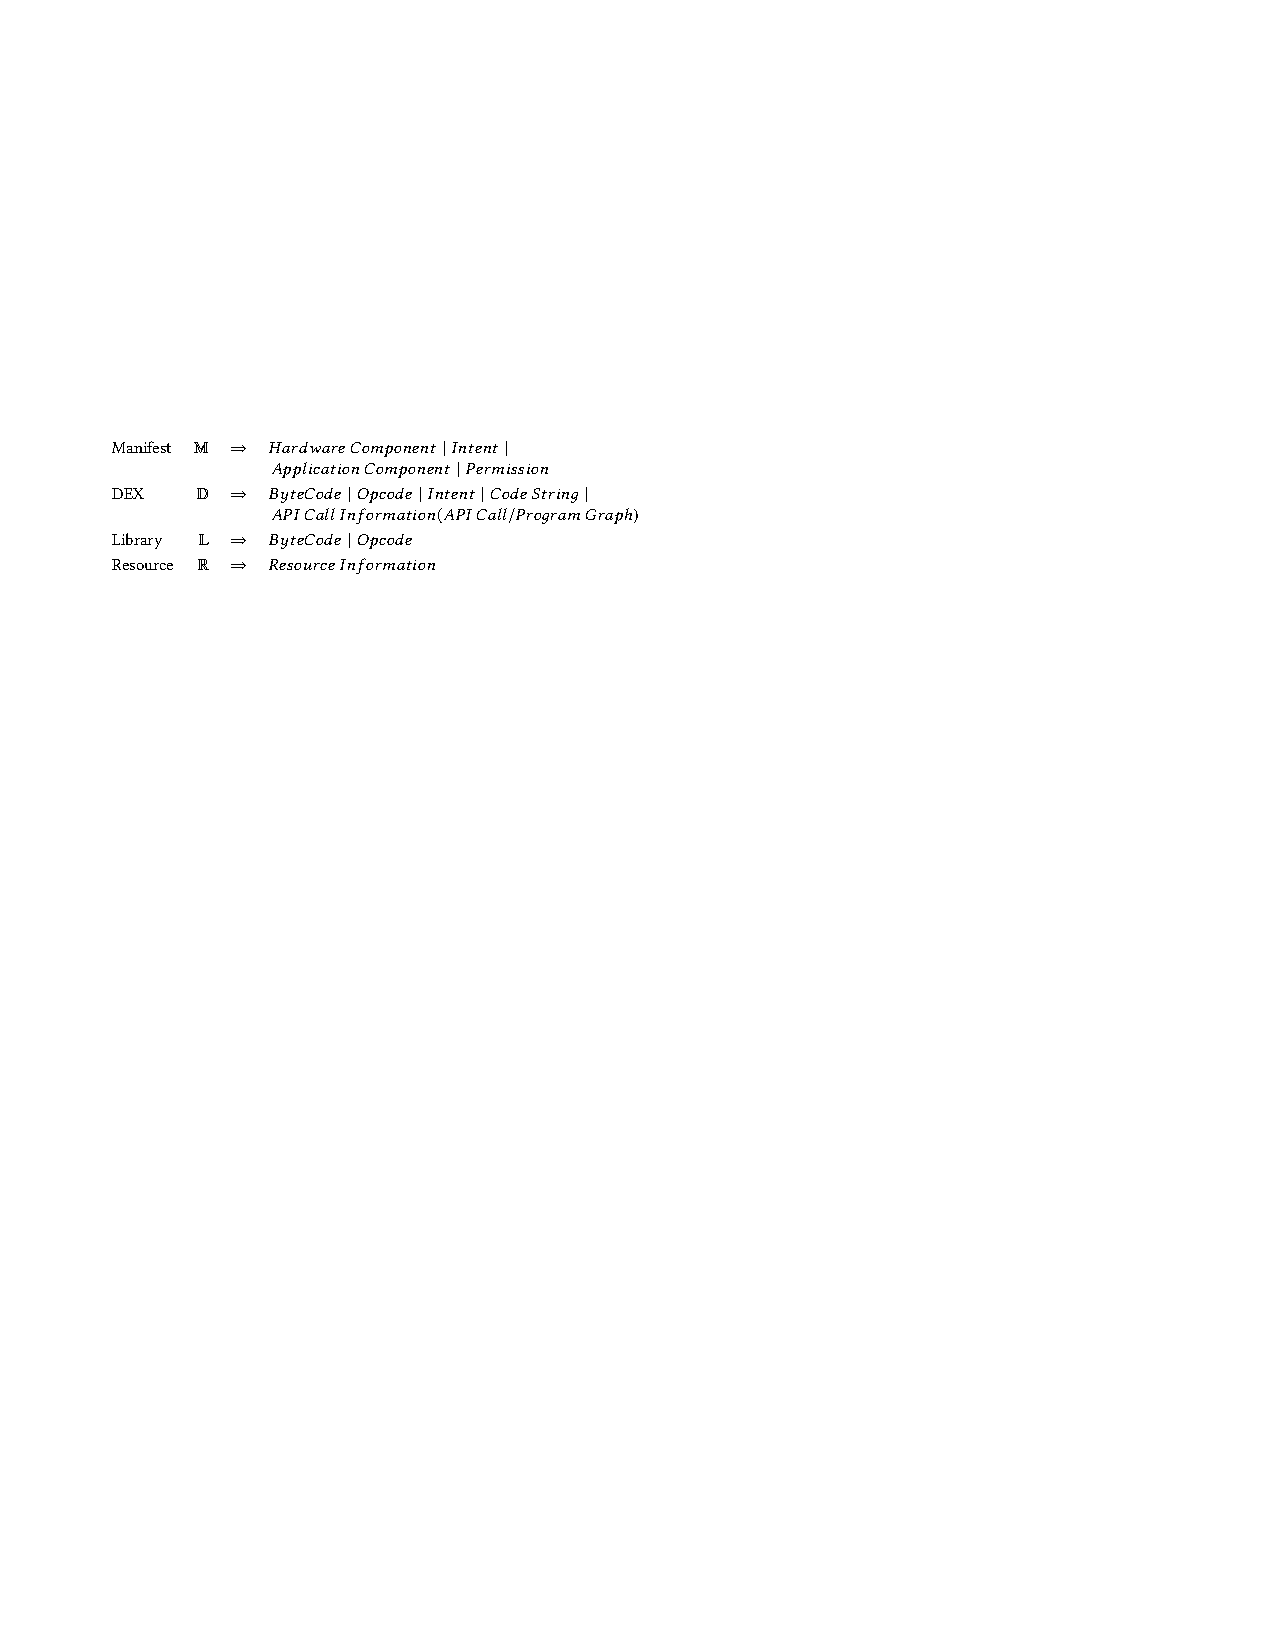
\includegraphics[width=0.73\linewidth]{fig/features.pdf}
%DIFDELCMD <     \vspace{-0.1cm}
%DIFDELCMD <     %%%
\DIFdelendFL \DIFaddbeginFL 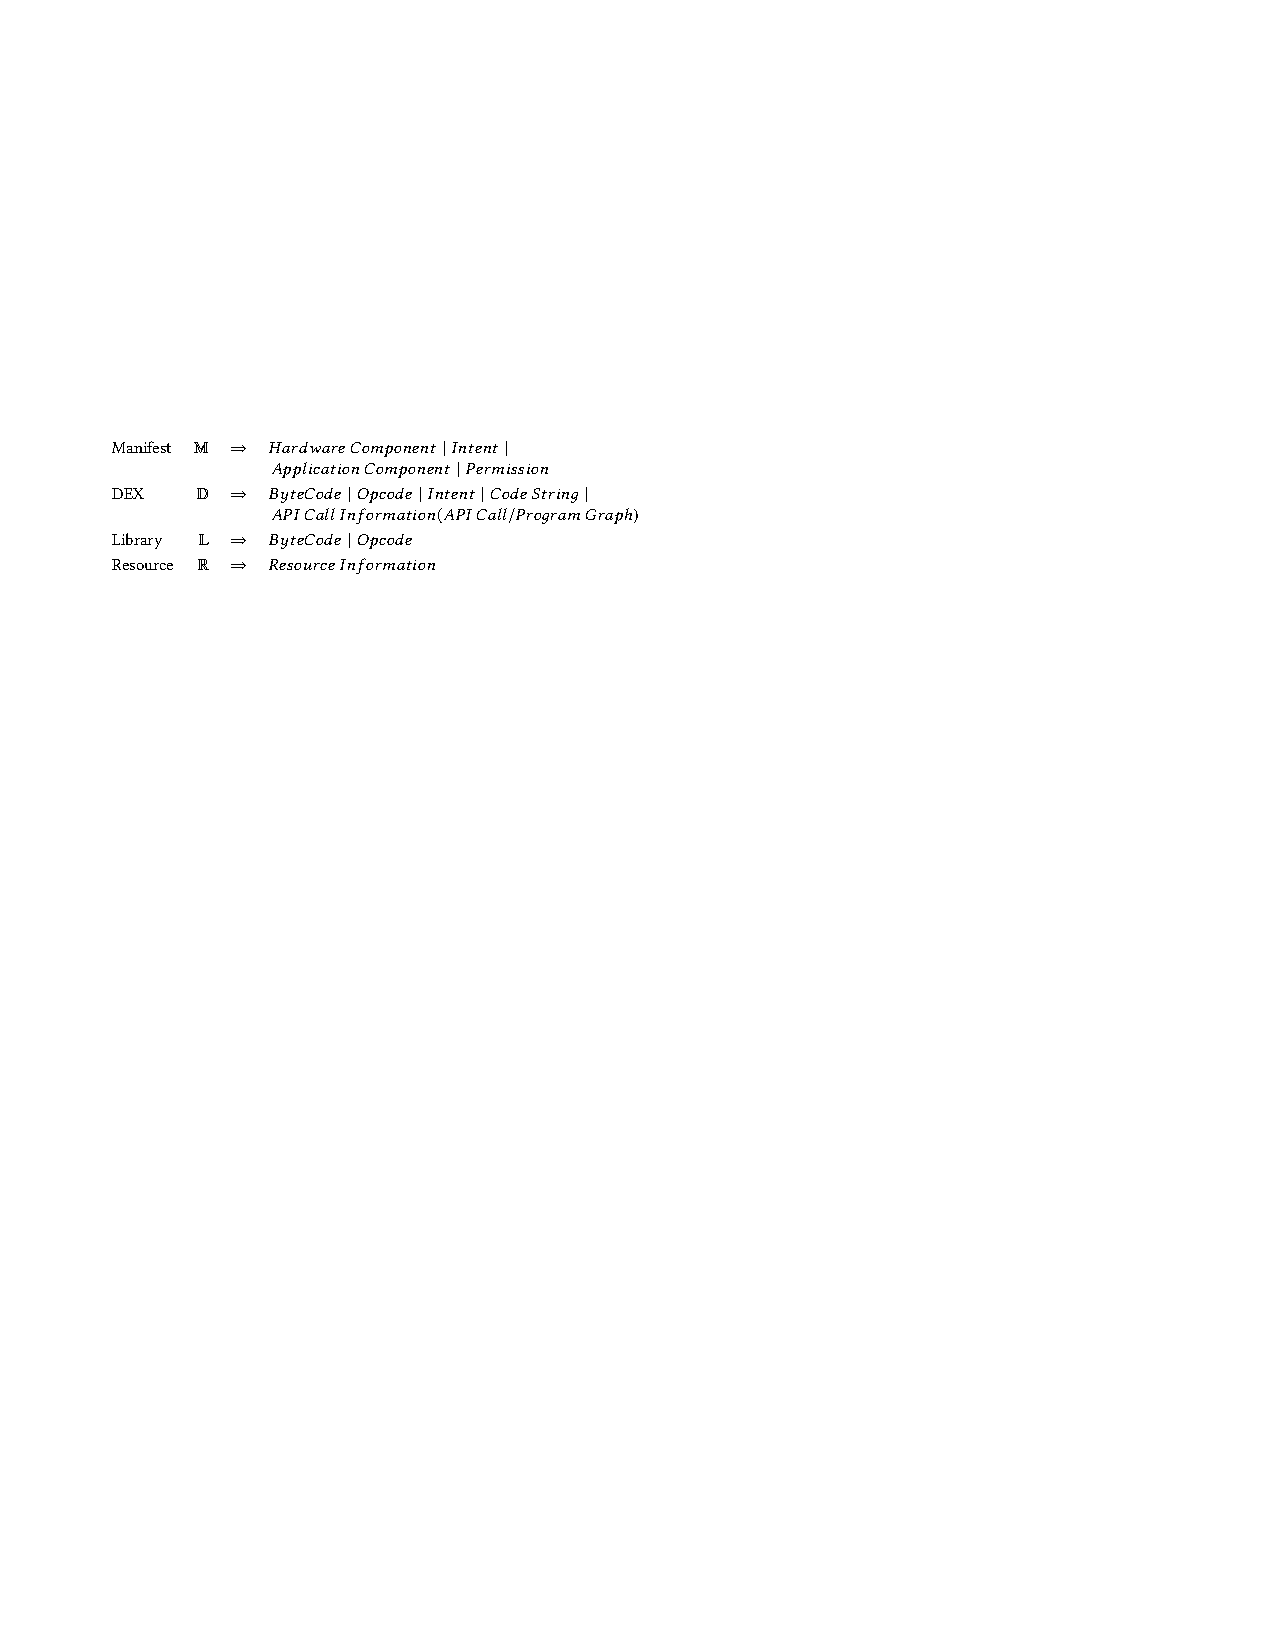
\includegraphics[width=0.66\linewidth]{fig/features.pdf}
    \vspace{-0.2cm}
    \DIFaddendFL \caption{APK files and their corresponding features.}
    \label{fig:features}
    \DIFdelbeginFL %DIFDELCMD < \vspace{-0.5cm}
%DIFDELCMD < %%%
\DIFdelendFL \DIFaddbeginFL \vspace{-0.6cm}
\DIFaddendFL \end{figure}

\featurepoint{[M|D]}{Intent}
As the primary ways of communication among components, intents connect various Application Components and delineate standard operations one app can perform.
% As the primary ways of communication among components, intents take responsibility for initiating Activities, managing Services lifecycle, and delivering information to Broadcast Receivers.
They are pivotal in initiating Activities, managing Services lifecycle, and delivering broadcast information to Broadcast Receivers.
Malware often monitors these communication status to trigger malicious actions, such as activating pre-configured malicious activities~\cite{zhou2012hey}.
Approaches~\cite{li2021robust,feng2020performance,xu2016iccdetector} aim to capture these malicious behaviors by analyzing corresponding intents.


% Towards this end, intents have been extensively employed to capture potential malicious activities~\cite{feng2020performance,li2021robust,xu2016iccdetector}.

% Approaches like MobiTive~\cite{feng2020performance} and RAMDA~\cite{li2021robust} utilize intents specified in the manifest for malware detection.
% Meanwhile, ICCDetector~\cite{xu2016iccdetector} integrates intents from the manifest and the application's codebase to model the application's behaviors.

\featurepoint{[M]}{Permission}
Android employs a permission-based mechanism to regulate access to sensitive data and restricted actions.
For an app to carry out particular actions, it must obtain the requisite permissions~\cite{au2012pscout,backes2016demystifying}.
The set of permissions required by an app can thus offer insights into its intended behaviors.
Particularly, malware often demands permissions that are unnecessary for benign apps to execute malicious actions~\cite{enck2009lightweight}.
Consequently, numerous Android malware detectors~\cite{he2022msdroid,xu2018deeprefiner,arp2014drebin,kim2018multimodal,wu2021android} capture the differences to distinguish malware. 


% Consequently, numerous malware detection frameworks~\cite{arp2014drebin,xu2018deeprefiner,kim2018multimodal,wu2021android,he2022msdroid} employ permissions as a key heuristic in distinguishing malware.


\featurepoint{[D]}{API Call Information (API Call and Program Graph)}
% \jiahao{Merge API call with its connections}
% \jh{API Call Information is a widely used feature source in Android malware detection, consisting of API calls and their connections.
% Android apps make use of API calls to tap into the operating system's functionality and system resources~\cite{peiravian2013machine}.
% For instance, calling the \textit{sendTextMessage()} indicates that the app is likely to send a text message.
% Additionally, the API calls are often connected with each other to form a program graph, where each node signifies a method, and each edge denotes a method invocation~\cite{li2023black}, illustrating the app's structural information~\cite{wu2019malscan}.}
% \red{For clarity, we decouple API Call Information into two sub-categories: \textit{API Call} refers to the API calls themselves, while \textit{Program Graph} denotes the connections between API calls.}
API Call Information, consisting of API calls and their connections, is a widely utilized feature source in Android malware detection.
Android apps make use of these API calls to access the operating system's functionality and system resources~\cite{peiravian2013machine}.
For instance, the invocation of \textit{sendTextMessage()} suggests that the app is likely to send a text message.
Furthermore, API calls are connected to form a graph, where each node signifies a method, and each edge denotes a method invocation~\cite{li2023black}, illustrating the app's structural information~\cite{wu2019malscan}.
For clarity, we differentiate API Call Information into two sub-categories: \textit{API Call}, referring to the individual API calls, and \textit{Program Graph}, denoting the relationships among these API calls.
Numerous studies~\cite{arp2014drebin,kim2018multimodal,wu2021android} detect sensitive API calls (\textit{e.g., getDeviceId()}) to estimate the probability of an app being malicious.
In contrast, other solutions~\cite{wu2019malscan,he2022msdroid,hou2017hindroid,xu2020sdac,martin2017evolving,ye2019out} venture deeper, examining the relationships between API calls to capture an app's semantics for malware detection.

\featurepoint{[D|L]}{ByteCode and Opcode}
Similar to previous research~\cite{xu2018deeprefiner,sun2016taintart,li2021palmtree,daoudi2021dexray}, we treat both the \textit{raw bytecode} and the \textit{assembly code} derived from the \textit{Dex} and \textit{Library} as ByteCode.
ByteCode contains a sequence of instructions, where each instruction consists of a single Opcode and several operands.
The Opcode denotes a specific operation; for instance, the \texttt{invoke} means a method invocation.
The operands provide additional information for the Opcode, such as the method name.
In addition, ByteCode and Opcode from the \textit{Dex} and \textit{Library} offer insights into the static execution flows of apps' Java and Native codes, providing a view of how an app work~\cite{kim2018multimodal}.
Recent research attempts to represent Bytecode and Opcode in various formats, such as image~\cite{mclaughlin2017deep,hsien2018r2,amin2022android,xiao2019image} and text~\cite{xu2018deeprefiner,yan2018lstm,karbab2021petadroid}, to capture apps' semantics.

% Consistent with previous studies~\cite{xu2018deeprefiner,sun2016taintart,li2021palmtree}, we consider the assembly code derived from the decompilation of DEX and Library files as another kind of bytecode representation of an application.
% Both bytecode and opcode preserve the original characteristics of an application, providing a holistic perspective on the programming behaviors the application executes.

\featurepoint{[D]}{Code String}
Apps often embed key information like URLs and IP addresses as string values within their codebase.
These strings can be traced in the assembly code, tagged either as \texttt{const-string} or \texttt{const-string/jumbo}. 
Such strings can provide crucial clues about potential malicious activities~\cite{arp2014drebin}.
For instance, malware sets up network sockets to communicate with remote servers, using the string \texttt{socket} in the codebase.
A number of works~\cite{arp2014drebin,kim2018multimodal,zhu2019transparent} have used code strings to identify potential illegal operations.

% With the evidence provided by research like~\cite{arp2014drebin,kim2018multimodal,zhu2019transparent}, it is clear that code string has become a significant feature in malware detection.

% Therefore, it is unsurprising that it has been widely adopted as a feature source in Android malware detection~\cite{arp2014drebin,kim2018multimodal,zhu2019transparent}.
% Accordingly, some approaches~\cite{arp2014drebin,kim2018multimodal,zhu2019transparent} have tapped into these strings as indicators for malware detection.

% \featurepoint{[D]}{Program Graph}
% The program graph encapsulates the caller-callee relationships among the methods inside an app as a directed graph, where each node signifies a method, and each edge denotes a method invocation~\cite{li2023black}.
% \jh{In essence, the program graph illustrates the app's structural information, 
% offering a holistic perspective on the app's behavior~\cite{wu2019malscan}.}
% When leveraging program graphs for malware detection, a prevalent strategy is to re-envision them as other constructs (\textit{e.g.}, as a social network) and subsequently employ corresponding techniques to extract valuable insights~\cite{wu2019malscan,wu2021homdroid}.
% Alternatively, some researchers directly apply powerful techniques, like graph neural network (GNN), to distill pertinent information from the program graph itself~\cite{mariconti2016mamadroid,he2022msdroid,gao2021gdroid}.

% To distill helpful information for malware detection, one popular selection is treating the program graph as a social network and apply related techniques to extract information~\cite{wu2019malscan,wu2021homdroid}.
% Another direction is to simplify the graph structure to capture meaningful information~\cite{mariconti2016mamadroid,he2022msdroid}.
% To utilize this information, one direction~\cite{wu2019malscan,wu2021homdroid} treats the program graph as a social network and performs centrality and homophily analysis~\cite{dehghani2016purity,fiore2005homophily}.
% Another direction is to simplify the graph structure to capture meaningful information~\cite{mariconti2016mamadroid,he2022msdroid}.
% There are also some approaches~\cite{} directly extract information from the program graph to detect malware.

% To preserve the program semantic information, MalScan~\cite{wu2019malscan} and HomDroid~\cite{wu2021homdroid} treat the program graph as a social network and perform centrality and homophily analysis~\cite{dehghani2016purity,fiore2005homophily}.

% Also, some approaches have attempted to simplify the graph structure to capture meaningful information. 
% For example, MamaDroid~\cite{mariconti2016mamadroid} abstracts the graph based on family and package details.
% MsDroid~\cite{he2022msdroid} derives subgraphs rooted with sensitive API calls to describe potential malicious operations.

\featurepoint{[R]}{Resource Information}
Apps utilize resources to house traditional files and static elements, such as bitmaps and animation instructions.
These resources are generally decoupled from the application codebase for ease of maintenance.
Attackers sometimes embed malicious code within resource files, like image files, as a tactic to evade detection.
Approaches like DeepRefiner~\cite{xu2018deeprefiner} consider resource information as a crucial feature source for malware detection.
% This stems from the fact that resources typically house traditional and static elements, such as bitmaps and animation instructions. 
% Attackers sometimes embed malicious code within resource files, like image files, as a tactic to evade detection.

% Resources refer to the traditional files and static elements leveraged by your application, such as bitmaps, layout definitions and animation instructions.
% These resources are generally decoupled from the application codebase for ease of maintenance. 
% During runtime, Android selects the most suitable resource based on the device's current configuration
% In some instances, attackers may insert malicious code into resource files, such as image files, as a tactic to elude detection.

% \featurepoint{[DY]}{Dynamic features}
% \jh{dynamic features are collected during runtime, and they are not included in the APK file. For example, the network traffic, the system traces, and the system calls. These information can reflected the app's runtime behaviors. It is time consuming to collect these features.}

\begin{figure}[t]
    \centering
    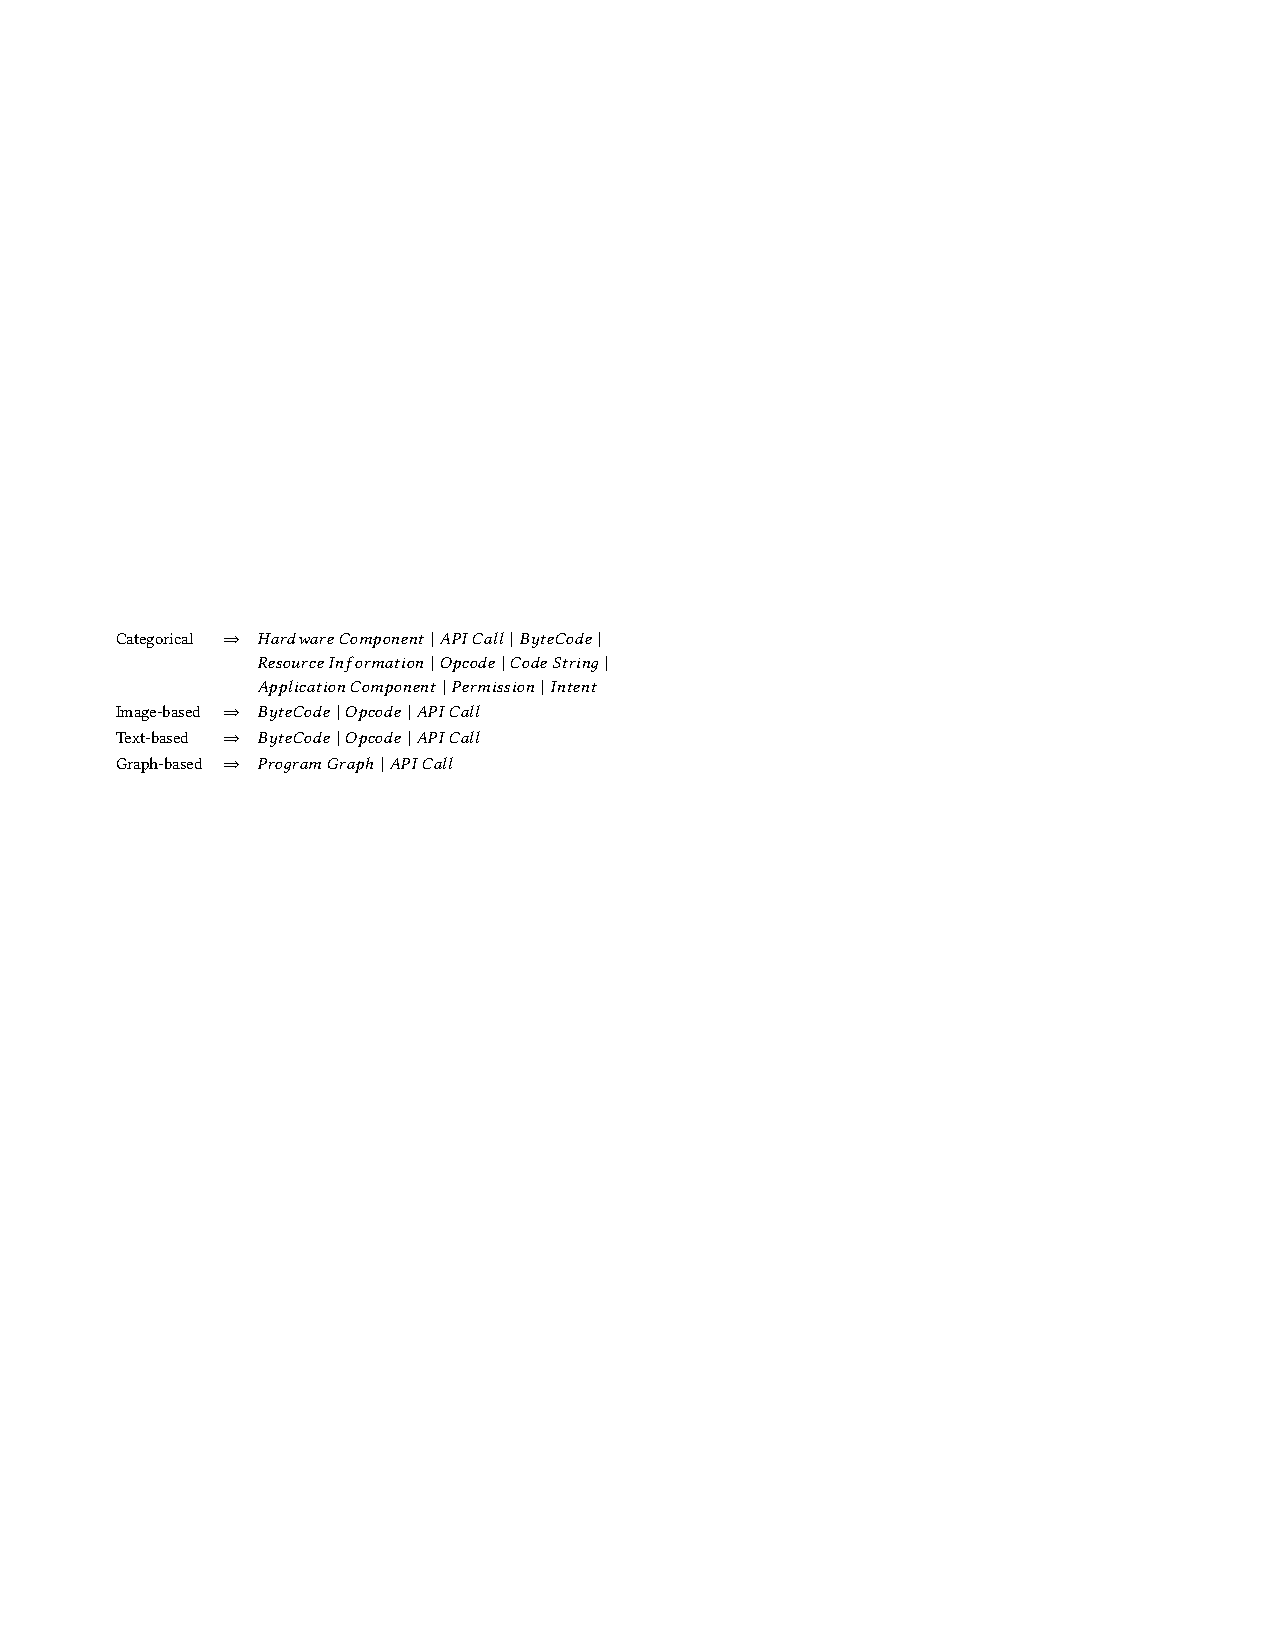
\includegraphics[width=0.68\linewidth]{fig/representation.pdf}
    \DIFdelbeginFL %DIFDELCMD < \vspace{-0.2cm}
%DIFDELCMD <     %%%
\DIFdelendFL \DIFaddbeginFL \vspace{-0.1cm}
    \DIFaddendFL \caption{The relationships between Feature Representations and widely used APK Features.}
    \label{fig:representation}
    \DIFdelbeginFL %DIFDELCMD < \vspace{-0.4cm}
%DIFDELCMD < %%%
\DIFdelendFL \DIFaddbeginFL \vspace{-0.5cm}
\DIFaddendFL \end{figure}

\subsection{Feature Representation}
\label{sub:apk_feature_encoding}
%DIF <  APK characterizations offer multi-perspective views of an app's behavior.
\DIFdelbegin \DIFdel{Before being fed into models, APK features }\DIFdelend \DIFaddbegin \DIFadd{APK characterizations provide multi-perspective views of an app's behavior.
Before these features can be fed into ML models, they }\DIFaddend must be encoded into \DIFdelbegin \DIFdel{a format that is interpretable by the models .
Specifically}\DIFdelend \DIFaddbegin \DIFadd{representations that the models can interpret.
Broadly}\DIFaddend , the encoding process \DIFdelbegin \DIFdel{can be organized }\DIFdelend \DIFaddbegin \DIFadd{falls }\DIFaddend into four categories: categorical, image-based, text-based, and graph-based.
\DIFdelbegin %DIFDELCMD < \jh{Figure~\ref{fig:representation} illustrates the relationships between these encoding strategies and specific APK features.}
%DIFDELCMD < %%%
\DIFdelend \DIFaddbegin \jh{Figure~\ref{fig:representation} illustrates the relationships between these encoding strategies and the corresponding APK features.}
\DIFaddend In the following section, we discuss \DIFdelbegin \DIFdel{these encoding strategies }\DIFdelend \DIFaddbegin \DIFadd{each encoding strategy }\DIFaddend in detail.

% Some approaches~\cite{yuan2014droid,arp2014drebin,li2019adversarial,feng2019mobidroid,li2021robust,wu2021android,hou2017hindroid} encode these features into a binary vector, where each position indicates whether a specific feature exists or not.
% Alternatively, another approach showcased in~\cite{kim2018multimodal} calculates the frequency of each feature to obtain a vector of real numbers.
\bulletpoint{Categorical encoding}
Features like hardware components, intents, and code strings are often viewed as categorical data and can be easily transformed into numerical values.
A widely-encoding strategy is to convert these features into a binary vector, where each position indicates whether a specific feature exists or not~\cite{arp2014drebin,hou2017hindroid,li2021robust,wu2021android,yuan2014droid,li2019adversarial,feng2019mobidroid}.
On the other hand, another line of research~\cite{kim2018multimodal} calculates the frequency of each feature to obtain a vector of numerical values, reflecting the importance of each feature.

\bulletpoint{Image-based encoding}
% Note: the bytecode definition
% Several approaches~\cite{daoudi2021dexray,ding2020android,mclaughlin2017deep,hsien2018r2,zegzhda2018applying,he2019malware,xiao2019image,yuan2020byte} depict bytecode or opcode sequences in the form of images, subsequently feeding them into a convolutional neural network (CNN) to extract features. 
% In Android malware detection, it is a prevalent practice to represent bytecode or opcode sequences as images.
% Various solutions~\cite{daoudi2021dexray,ding2020android,hsien2018r2,xiao2019image,mclaughlin2017deep} visualize the bytecode or opcode sequences as image forms, subsequently extracting information from these depictions.
% Notably, \textsc{DexRay}~\cite{daoudi2021dexray} transforms the app's bytecode into grey-scale vector images, wherein each pixel corresponds to a distinct byte.
% Additionally, some approaches map various features to images to represent the APK. 
% For instance, Zegzhda et al.~\cite{zegzhda2018applying} attempt to map the sequence of API calls combined with protection levels to an RGB image.
Representing specific features as images and leveraging image processing techniques is a well-established approach in malware detection.
Specifically, bytecode and opcode are often visualized as images to describe apps' behaviors~\cite{mclaughlin2017deep,daoudi2021dexray,hsien2018r2,xiao2019image,ding2020android}.
Notably, \textsc{DexRay}~\cite{daoudi2021dexray} transforms the app's bytecode into grey-scale vector images, wherein each pixel corresponds to a distinct byte.
In a similar vein, some other features are also mapped to images to depict the APK's characteristics.
For instance, Zegzhda et al.~\cite{zegzhda2018applying} combine API calls with protection levels as an RGB image.

\bulletpoint{Text-based encoding}
% Bytecode and opcode sequences can be analogized to textual data.
% Many existing approaches~\cite{xu2018deeprefiner,karbab2018maldozer,karbab2021petadroid,xu2020sdac,sun2019scalable} regard apk characterization as textual data and leverage natural language processing (NLP) techniques to enhance android malware detection.
% By considering API calls as \texttt{words} and their sequences as \texttt{sentences}, methods presented in~\cite{karbab2018maldozer,karbab2021petadroid,xu2020sdac} utilize word embedding techniques, such as Word2Vec~\cite{mikolov2013distributed}, to extract semantic information included in the API calls.
% Separately, Sun et al.~\cite{sun2019scalable} treat API calls and permissions as sparse data, applying Doc2Vec~\cite{le2014distributed} to derive their vector representations.
Text-based encoding is also a widely used strategy in Android malware detection.
Many existing methods~\cite{xu2018deeprefiner,xu2020sdac,karbab2021petadroid,karbab2018maldozer,sun2019scalable} have approached APK features from a textual perspective, employing natural language processing (NLP) techniques to amplify detection capability.
For example, by considering API calls as \texttt{words} and their sequences as \texttt{sentences}, methods presented in~\cite{xu2020sdac,karbab2021petadroid,karbab2018maldozer} utilize word embedding techniques, such as Word2Vec~\cite{mikolov2013distributed}, to extract semantic information included in the API calls.
\DIFaddbegin \DIFadd{Separately, Sun et al.~\mbox{%DIFAUXCMD
\cite{sun2019scalable} }\hskip0pt%DIFAUXCMD
treat API calls and permissions as sparse data, applying Doc2Vec~\mbox{%DIFAUXCMD
\cite{le2014distributed} }\hskip0pt%DIFAUXCMD
to derive their vector representations.
}\DIFaddend 

\bulletpoint{Graph-based encoding}
Recently, graph structure has been widely adopted to represent apps' semantics~\cite{he2022msdroid,li2023black}.
One direction is to leverage program graphs to model APK behaviors~\cite{wu2019malscan,wu2021homdroid,he2022msdroid,pektacs2020deep,pektacs2020learning}.
Another avenue aims to build API-based feature graphs, drawing insights from API calls and their meta-relationships. 
An example is to identify whether two API calls are in the same block, thereby capturing the app's intended operations~\cite{hou2017hindroid,huang2019deep}.
When these features are represented as graphs, graph-based techniques (\textit{e.g.,} Graph2Vec~\cite{narayanan2017graph2vec}, social network~\cite{wu2019malscan}) are employed to extract apps's structural information.



% \vspace{-0.1cm}
\subsection{Machine Learning Modeling}
\label{sub:ml_models}
% Subsequent to encoding, learning models are leveraged to identify underlying patterns from the encoded features, facilitating informed predictions.
After encoding these features as numerical vectors, machine learning models are leveraged to identify malicious patterns.
Following previous studies~\cite{qiu2020survey,zhao2021impact}, we categorize the models employed in Android malware detection into two main categories: traditional machine learning (TML) and deep learning (DL) models.
TML models, such as linear regression or decision trees, typically exhibit simpler structures that can explicitly model the relationship between input and output. 
As such, these TML models often require domain knowledge to extract features from input data.
In contrast, DL models are characterized by their multiple layers of neurons, enabling them to capture complex non-linear mappings from input to output~\cite{zhao2018deepsim}.
This capability means that DL models are less reliant on domain knowledge during the feature extraction.
In this section, we provide a concise introduction to the widely used models.
%  in Android malware detection.

\bulletpoint{TML models}
% SVM~\cite{arp2014drebin,hou2017hindroid,xu2020sdac,sun2016sigpid,garcia2018lightweight}
% KNN~\cite{wu2019malscan,wu2021homdroid,wu2016effective,aafer2013droidapiminer}
% RF~\cite{mariconti2016mamadroid,zhu2018hemd}
% DT~\cite{zarni2013permission,yerima2014android}
% (SVM)~\cite{noble2006support}
% (KNN)~\cite{peterson2009k} (RF)~\cite{breiman2001random}
Given APK features, TML models are commonly employed to discern patterns from them.
The Support Vector Machine (SVM) can find one hyperplane that separates the high-dimension data points with varying labels.
This capability has made it a popular choice to detect Android malware~\cite{arp2014drebin,hou2017hindroid,xu2020sdac,sun2016sigpid,garcia2018lightweight}.
K-Nearest Neighbors (KNN) has also been applied in Android malware detection~\cite{wu2019malscan,wu2021homdroid,aafer2013droidapiminer,wu2016effective}.
This algorithm identifies the nearest neighbors of a given sample and subsequently classifies the sample based on the majority label of its neighbors.
Additionally, as an ensemble-based learning method, Random Forest (RF) creates a forest of decision trees, each trained on a random subset of the data.
This approach capitalizes on the strength of multiple decision trees, making the model more robust and accurate than individual trees.
Such advantages have led to its significant application in malware detectors~\cite{mariconti2016mamadroid,zhu2018hemd}.

\bulletpoint{DL models}
DL models have exhibited strong capability in modeling malware behaviors. 
This part provides an insight into the widely used DL models tailored for Android malware detection.
% Multi-Layer Perceptron (MLP) is a fundamental model composed of multiple layers of neurons and has been applied in various studies~\cite{kim2018multimodal,li2021robust,martin2017evolving,sun2019scalable,zhu2019fsnet,chen2020denas}.
As a basic feed-forward neural network, Multi-Layer Perceptron (MLP), composed of several layers of neurons, \jh{has shown significant effectiveness in detecting Android malware~\cite{kim2018multimodal,li2021robust,martin2017evolving,sun2019scalable,zhu2019fsnet,chen2020denas}.}
The Recurrent Neural Network (RNN)~\cite{medsker2001recurrent} is a type of neural architecture that can capture the sequential information of input data.
By representing APK features (\textit{e.g.}, API calls and bytecode) as sequences, existing solutions~\cite{xu2018deeprefiner,yan2018lstm,vinayakumar2017deep} leverage RNN to explore the temporal dependencies embedded in these features.
The Convolutional Neural Network (CNN)~\cite{he2017mask} is equipped with multiple convolutional and pooling layers, enabling it to recognize contextual information derived from low-level features~\cite{girshick2015fast}.
%DIF <  This intrinsic capability makes it especially effective in capturing patterns from image-oriented data.
\DIFaddbegin \DIFadd{This intrinsic capability makes it especially effective in capturing patterns from image-oriented data.
}\DIFaddend Reflecting its efficacy, CNN has been extensively employed to extract malicious patterns from image-based features in Android malware detection~\cite{mclaughlin2017deep,hsien2018r2,feng2019mobidroid,karbab2018maldozer,huang2019deep,he2019malware}.
Given the graph representation of APK features (\textit{e.g.,} program graphs), Graph Neural Network (GNN)~\cite{kipf2016semi} can facilitate malware detection~\cite{he2022msdroid,mariconti2016mamadroid,gao2021gdroid,fan2021heterogeneous}.
This is because GNN can effectively propagate and aggregate node information along graph edges, thereby capturing the structural information of apps.
%DIF >  some approaches~\cite{he2022msdroid,gao2021gdroid,fan2021heterogeneous} have attempted to tailor Graph Neural Networks (GNN) to facilitate malware detection.
Utilizing a process of encoding and subsequently decoding input features, Autoencoders (AE) have the capacity to generate refined data representations, which makes it a popular choice in detecting malware~\cite{li2021robust,yang2021cade,zhu2021hybrid}.

In addition, existing research~\cite{su2016deep,wang2020sedroid,amin2022android} also tries to explore the potential of other DL models, like generative adversarial network (GAN)~\cite{goodfellow2014generative} and deep belief network (DBN)~\cite{hinton2009deep}.
For instance, Amin et al.~\cite{amin2022android} employ the dual-network structure of GAN --- one generates malware samples and the other works to distinguish these samples --- to enhance the malware detection capability.


% \begin{center}
%     \begin{conclusionbox}
%DIF <      \textit{Observation:} 
%DIF >      \textit{Finding:} 
%     \jh{Central to static and ML-based Android malware detection is how to effectively \textit{profile apps' behaviors} and how to \textit{leverage suitable ML models} to unveil malicious patterns.}
%     \end{conclusionbox}
% \end{center}

%DIF <  some approaches~\cite{he2022msdroid,gao2021gdroid,fan2021heterogeneous} have attempted to tailor Graph Neural Networks (GNN) to facilitate malware detection.
\DIFaddbegin \begin{center}
    \begin{conclusionbox}
    \textit{\DIFadd{Finding:}} 
    \jh{At the core of static and ML-based Android malware detection lies the ability to accurately \textit{profile app behaviors} and to \textit{select and leverage appropriate ML models} that can effectively uncover malicious patterns. Achieving this requires not only expressive feature representations but also a careful alignment between behavioral semantics and model capabilities.}
    \end{conclusionbox}
\end{center}

\DIFaddend % \subsection{Summary}
% \label{sub:summary}
% Quick summarize this section, and use some motivation to illustrate we need to conduct a quantitative analysis on the primary techniques.


% \begin{table*}[t]
% \centering
% \caption{
% % (\textit{AndroidManifest.xml} for Manifest, \textit{classes*.dex} for Dex, \textit{res/*} for Resource, and \textit{*.so} for Library)
% An overview of the 12 representative approaches we selected from major venues in security, software engineering, and machine learning. 
% \ymark \ indicates that the APK file (e.g., \textit{AndroidManifest.xml} for Manifest) is taken as input in Android malware detection, while \nmark \ is the opposite.
% \cmark \ and \xmark \ indicate whether feature engineering is handcrafted using domain knowledge or learned using representation learning.
% The effectiveness we present is based on the results reported in the original papers.}
% \begin{adjustbox}{width=0.85\linewidth}
% \begin{tabular}{@{}c|cc|cccc|cc|rr|rrr@{}}
% \toprule
% \multirow{2}{*}{\raisebox{-0.3cm}{\textbf{\begin{tabular}[c]{@{}c@{}}Selected \\ Approach\end{tabular}}}} & \multicolumn{2}{c|}{\textbf{Publication}} & \multicolumn{4}{c|}{\textbf{Input from APK}} & \multicolumn{2}{c|}{\textbf{Feature Engineering}} & \multicolumn{2}{c|}{\textbf{Dataset}} & \multicolumn{3}{c}{\textbf{Effectiveness}} \\ \cmidrule(lr){2-3} \cmidrule(lr){4-7} \cmidrule(lr){8-9} \cmidrule(lr){10-11} \cmidrule(l){12-14}
%  & \textbf{Venue} & \textbf{Year} & \textbf{Manifest} & \textbf{Dex} & \textbf{Resource} & \textbf{Library} & \textbf{Handcrafted} & \textbf{Learned} & \textbf{Malware} & \textbf{Goodware} & \textbf{TPR} & \textbf{FPR} & \textbf{F1} \\ \midrule
% Drebin\cite{arp2014drebin} & NDSS & 2014 & \ymark & \ymark & \nmark & \nmark & \cmark & \xmark & 5,560 & 123,453 & 94\% & \textbf{1\%} & 87\% \\ \midrule
% % ICCDetector\cite{xu2016iccdetector} & TIFS & 2016 & \ymark & \ymark & \nmark & \nmark & & & 5,264 & 12,026 & 93\% & \textbf{1\%} & 96\% \\ \midrule
% MamaDroid\cite{mariconti2016mamadroid} & NDSS & 2017 & \nmark & \ymark & \nmark & \nmark & \cmark & \xmark & 35,493 & 8,447 & 97\% & 2\% & 96\% \\ \midrule
% Mclaughlin et al.\cite{mclaughlin2017deep} & CODASPY & 2017 & \nmark & \ymark & \nmark & \nmark & \xmark& \cmark & 13,637 & 13,758 & 95\% & \textbf{1\%} & 97\% \\ \midrule
% HinDroid\cite{hou2017hindroid} & KDD & 2017 & \nmark & \ymark & \nmark & \nmark & \cmark & \xmark & 1,216 & 1,118 & \textbf{99\%} & 2\% & \textbf{99\%} \\ \midrule
% DeepRefiner\cite{xu2018deeprefiner} & EuroS\&P & 2018 & \ymark & \ymark & \ymark & \nmark & \xmark & \cmark & 62,915 & 47,525 & 98\% & 2\% & 98\% \\ \midrule
% Kim et al.\cite{kim2018multimodal} & TIFS & 2018 & \ymark & \ymark & \nmark & \ymark & \cmark & \cmark & 21,260 & 20,000 & \textbf{99\%} & \textbf{1\%} & \textbf{99\%} \\ \midrule
% MalScan\cite{wu2019malscan} & ASE & 2019 & \nmark & \ymark & \nmark & \nmark & \cmark & \xmark & 15,430 & 15,285 & --- & --- & 98\% \\ \midrule
% SDAC\cite{xu2020sdac} & TDSC & 2020 & \nmark & \ymark & \nmark & \nmark & \xmark & \cmark & 34,497 & 35,645 & 98\% & \textbf{1\%} & \textbf{99\%}\\ \midrule
% HomDroid\cite{wu2021homdroid} & ISSTA & 2021 & \nmark & \ymark & \nmark & \nmark & \cmark & \xmark & 3,358 & 4,840 & 97\% & 4\% & 95\% \\ \midrule
% Xmal\cite{wu2021android} & TOSEM & 2021 & \ymark & \ymark & \nmark & \nmark & \cmark & \xmark & 15,570 & 20,120 & 98\% & 2\% & 98\% \\ \midrule
% RAMDA\cite{li2021robust} & WWW & 2021 & \ymark & \ymark & \nmark & \nmark & \cmark & \xmark & 21,621 & 36,862 & 93\% & \textbf{1\%} & 90\% \\ \midrule
% MSDroid\cite{he2022msdroid} & TDSC & 2022 & \nmark & \ymark & \nmark & \nmark & \cmark & \xmark & 30,210 & 51,580 & 97\% & \textbf{1\%} & 97\% \\ \bottomrule
% \end{tabular}
% \end{adjustbox}
% \centering
% \begin{tablenotes}
% \footnotesize
% \item \ \ TPR, FPR, and F1 refer to true positive rate, false positive rate, and F1-score. 
% As MalScan is only evaluated on F1, its TPR and FPR are not available.
% \end{tablenotes}
% \label{tab:literature}
% \vspace{-0.4cm}
% \end{table*}

\section{\codename}
\label{sec:framework}

% The architecture of \codename is depicted in Figure~\ref{fig:framework}. 
% Beginning with a dataset of Android apps, the first step is to extract pertinent features from these apps.
% These features are then meticulously stored in a feature database. More details are provided in~\ref{sub:feature_db}.
% Subsequently, a dedicated preprocessor is utilized to transform (including retrieving and encoding) these features.
% After that, we proceed to train an ML model and assess its performance in detecting malware.

% % The framework is crafted with two guiding principles at its core: modularization and flexibility.
% \codename is designed with modularity in mind, making it easy to extend and customize.
% This is achieved by decoupling it into three distinct modules: \textit{feature database}, \textit{preprocessor}, and \textit{ML model}.
% Given the structured format of the \textit{feature database}, one can easily incorporate new features and integrate them into the assessment pipeline.
% Moreover, the \textit{preprocessor} can be tailored to accommodate various approaches, granting users the flexibility to determine what/how features are used.
% The \textit{ML model} is preloaded with various ML models, such as SVM, MLP, CNN, and AE.
% Alternatively, \codename also supports custom models, allowing users to incorporate their own models into the framework.

% \begin{figure}[t]
%     \centering
%     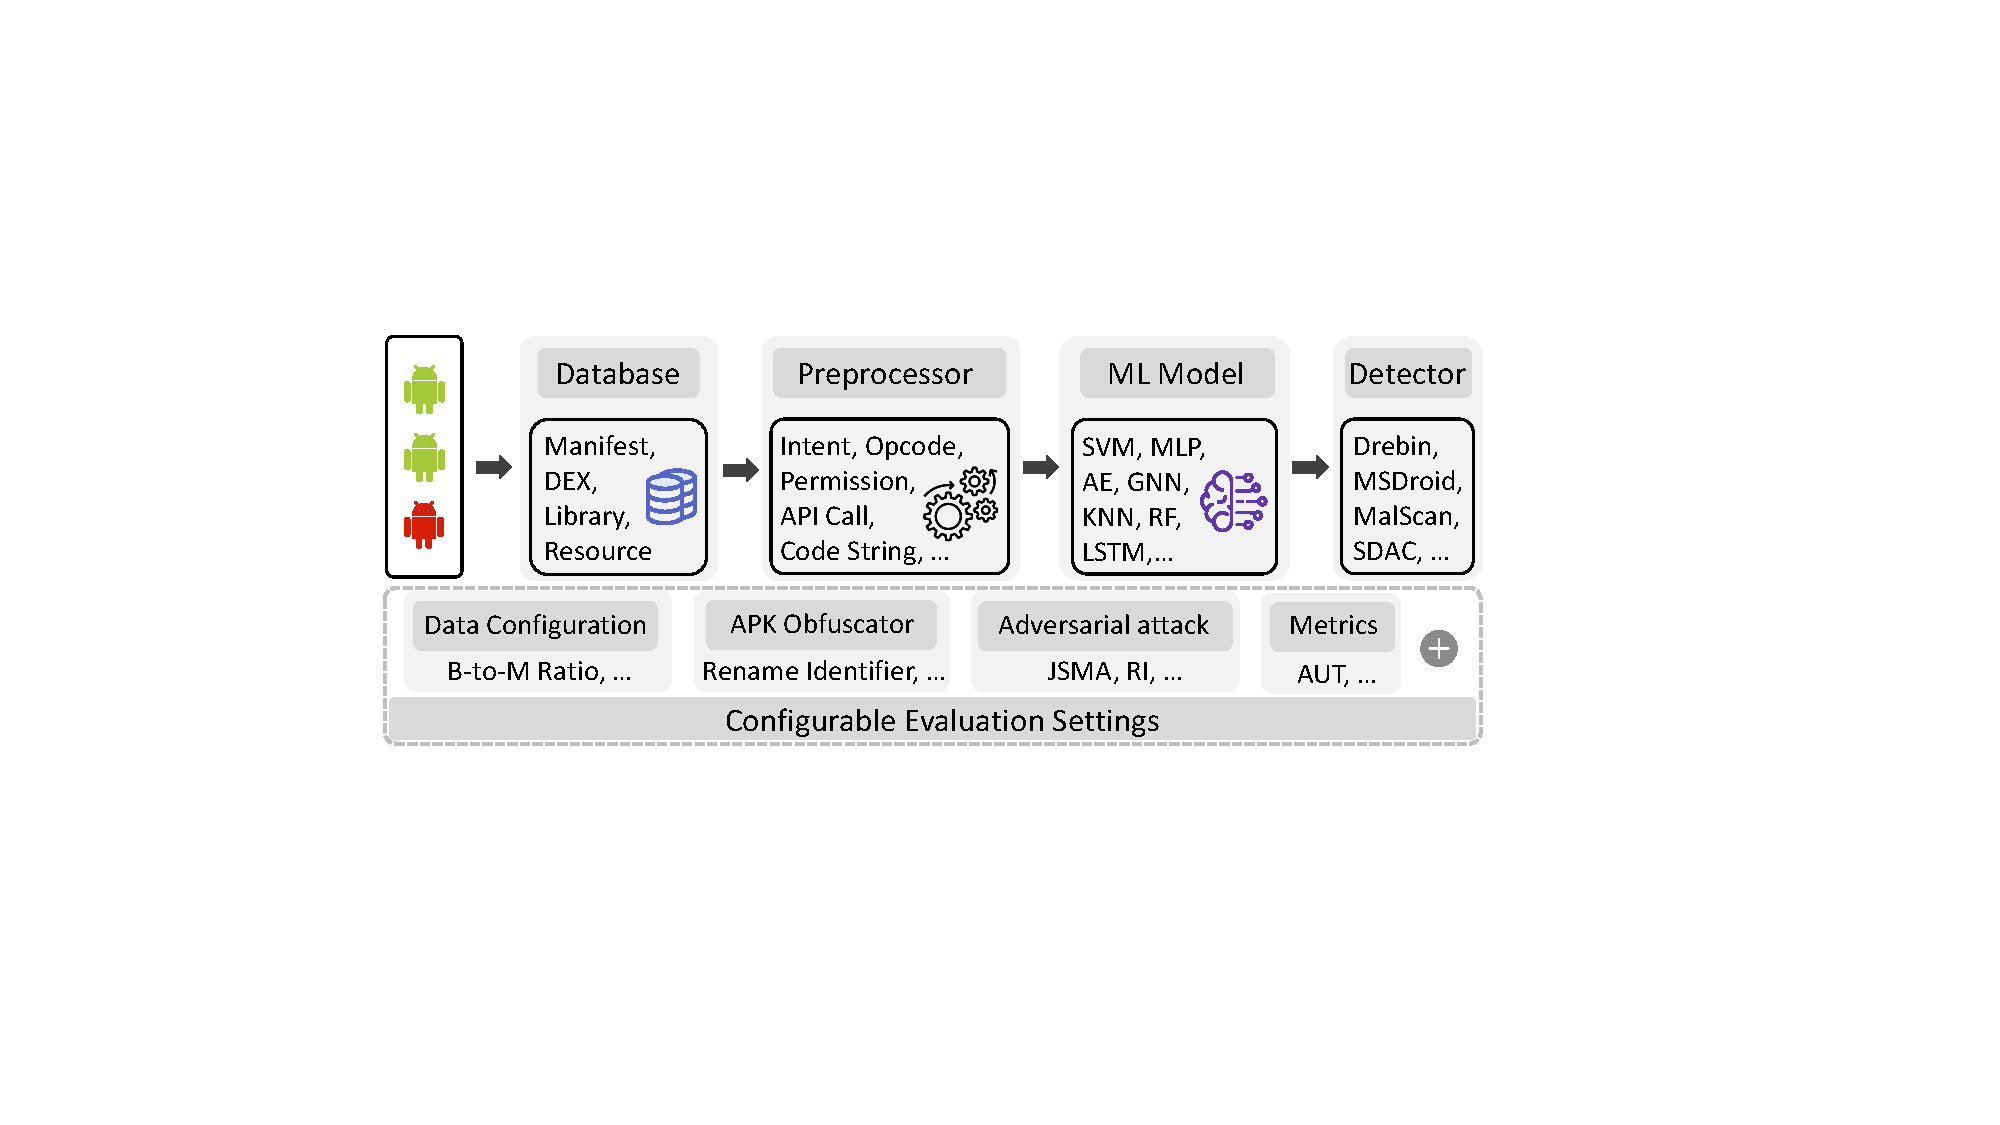
\includegraphics[width=0.94\linewidth]{fig/framework.pdf}
%     \caption{The architecture of \codename.}
%     \label{fig:framework}
%     % \vspace{-0.6cm}
% \end{figure}

% % Following the feature storing format in the {\em feature database}, it is easy to aggregate new features into the framework.
% % With this design, it is easy to design an additional feature extractor and store the derived features in the {\em feature database}, ensuring a smooth integration into the assessment pipeline.
% % Additionally, the {\em preprocessor} can be tailored to accommodate various approaches, granting users the flexibility to choose and adapt feature usage as required.
% \codename also provides a configurable experimental setting to support a wide range of evaluation scenarios.
% Parameters such as the ratio of goodware-to-malware, training data sizes, and time decay are all adjustable.
% This enables users to meticulously select APK samples for diverse evaluation contexts, ensuring comprehensive and accurate assessments.
% Moreover, \codename integrates an APK obfuscator~\cite{aonzo2020obfuscapk}, allowing for obfuscation prior to feature extraction. 
% It also possesses the capability to produce adversarial samples, enabling a robust assessment of model resilience.
% % Leveraging the capabilities of \codename, we re-implement the approaches described in Section~\ref{sec:approach_analysis} and assess them with our curated dataset.
% % We further analyze the evaluation outcomes to provide deeper insights into the current ML-based Android malware detection in Section~\ref{sec:evaluation}.

% % \bulletpoint{Implementation}
% % \codename is developed in 17K lines of Python code.
% % To ensure consistency and mitigate biases from different feature extraction toolchains and learning frameworks, we adopt standardized techniques across all tasks.
% % For feature extraction, we use Androguard to disassemble APK files and derive features such as permissions, intents, and program graphs. 
% % LibRadar helps in identifying third-party libraries within the applications, while Angr is used for analyzing native libraries and capturing essential features like opcodes and API calls. 
% % When it comes to training ML models, the scikit-learn library is our choice for traditional ML algorithms like SVM, KNN, and RF.
% % On the other hand, for DL architectures such as CNN, LSTM, GNN, and AE, we resort to Pytorch.
% % This uniform approach ensures a balanced evaluation, concentrating purely on the uniqueness and performance of each method.
% % Details about the hyper-parameters of these models are provided in Appendix~\ref{sub:hyperparameters}.

\begin{figure}[t]
    \centering
    \DIFdelbeginFL %DIFDELCMD < 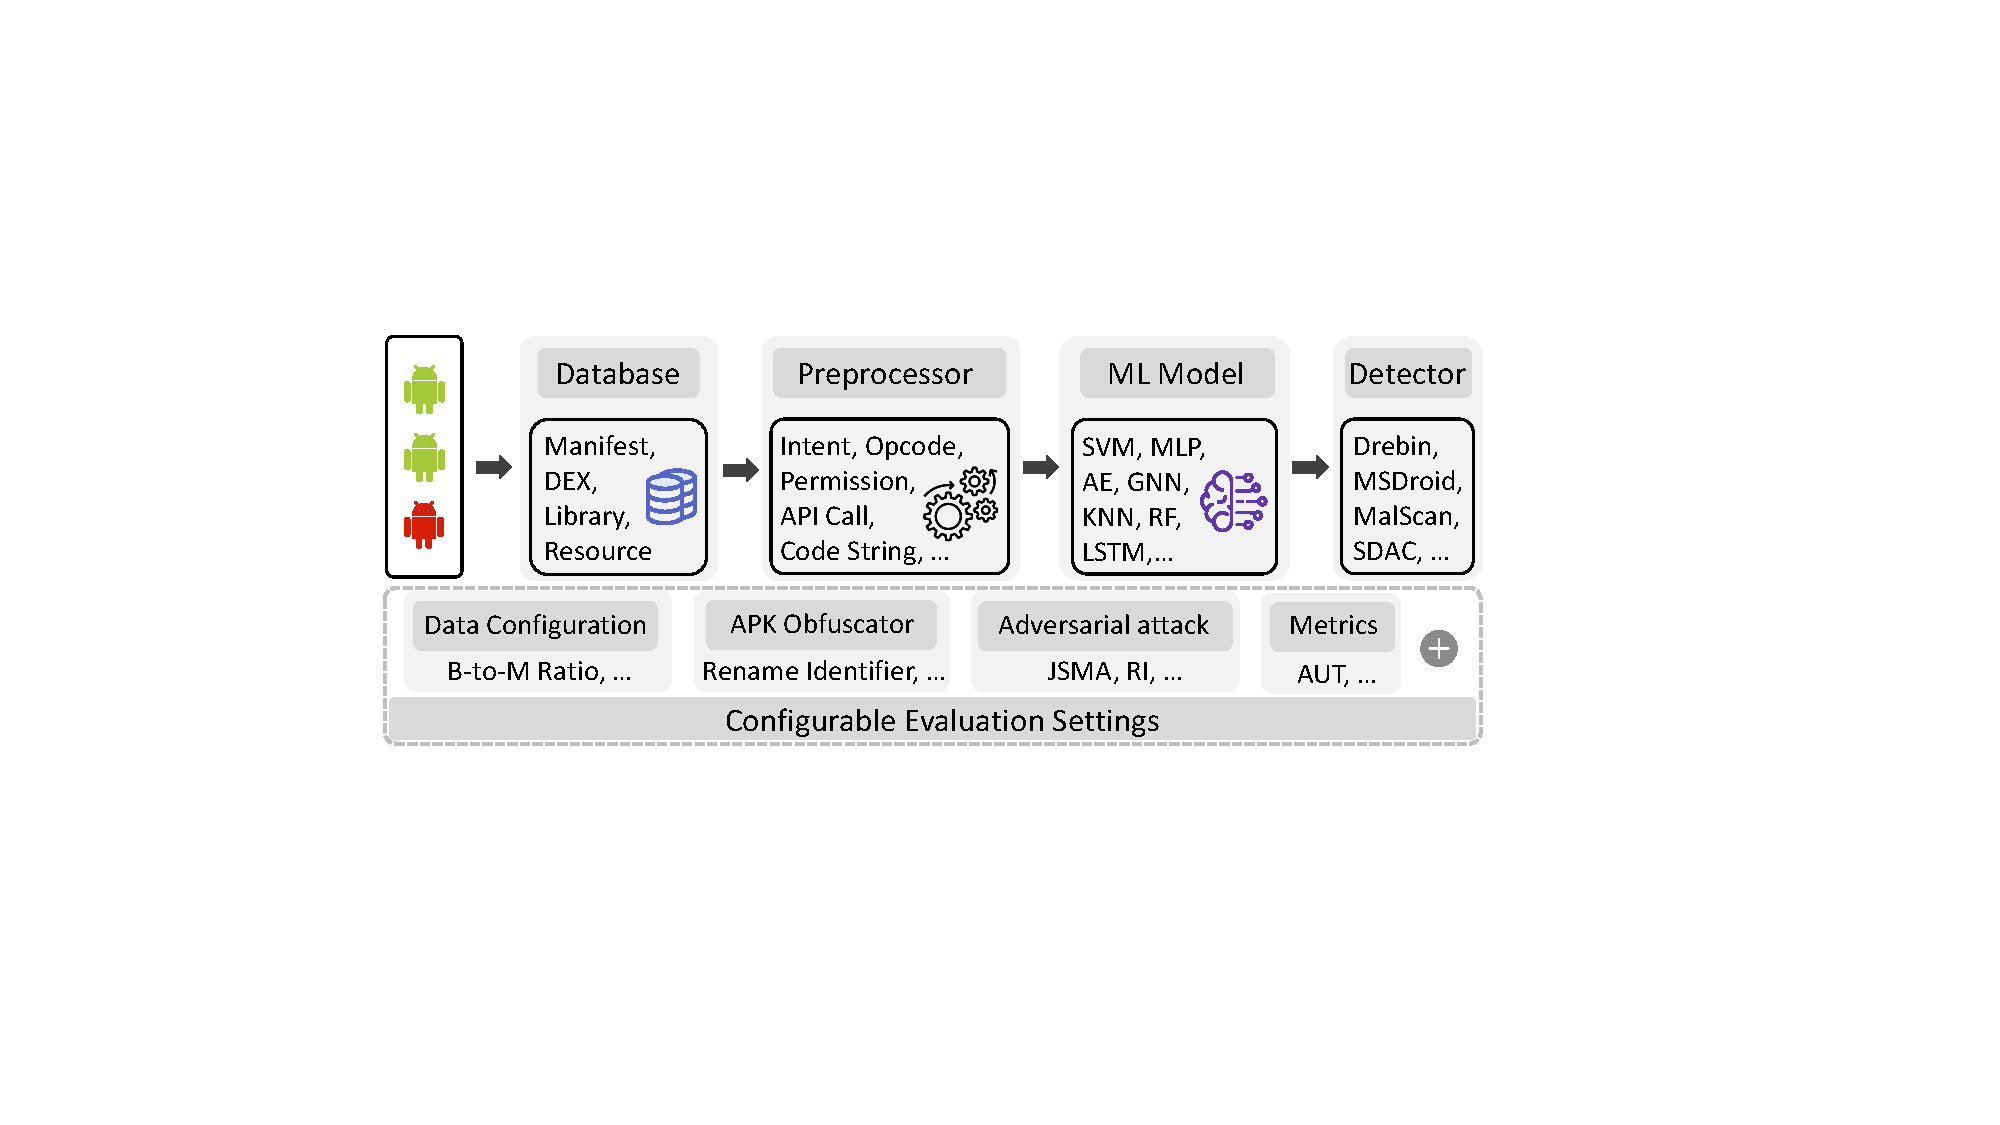
\includegraphics[width=0.74\linewidth]{fig/framework.pdf}
%DIFDELCMD <     %%%
\DIFdelendFL \DIFaddbeginFL 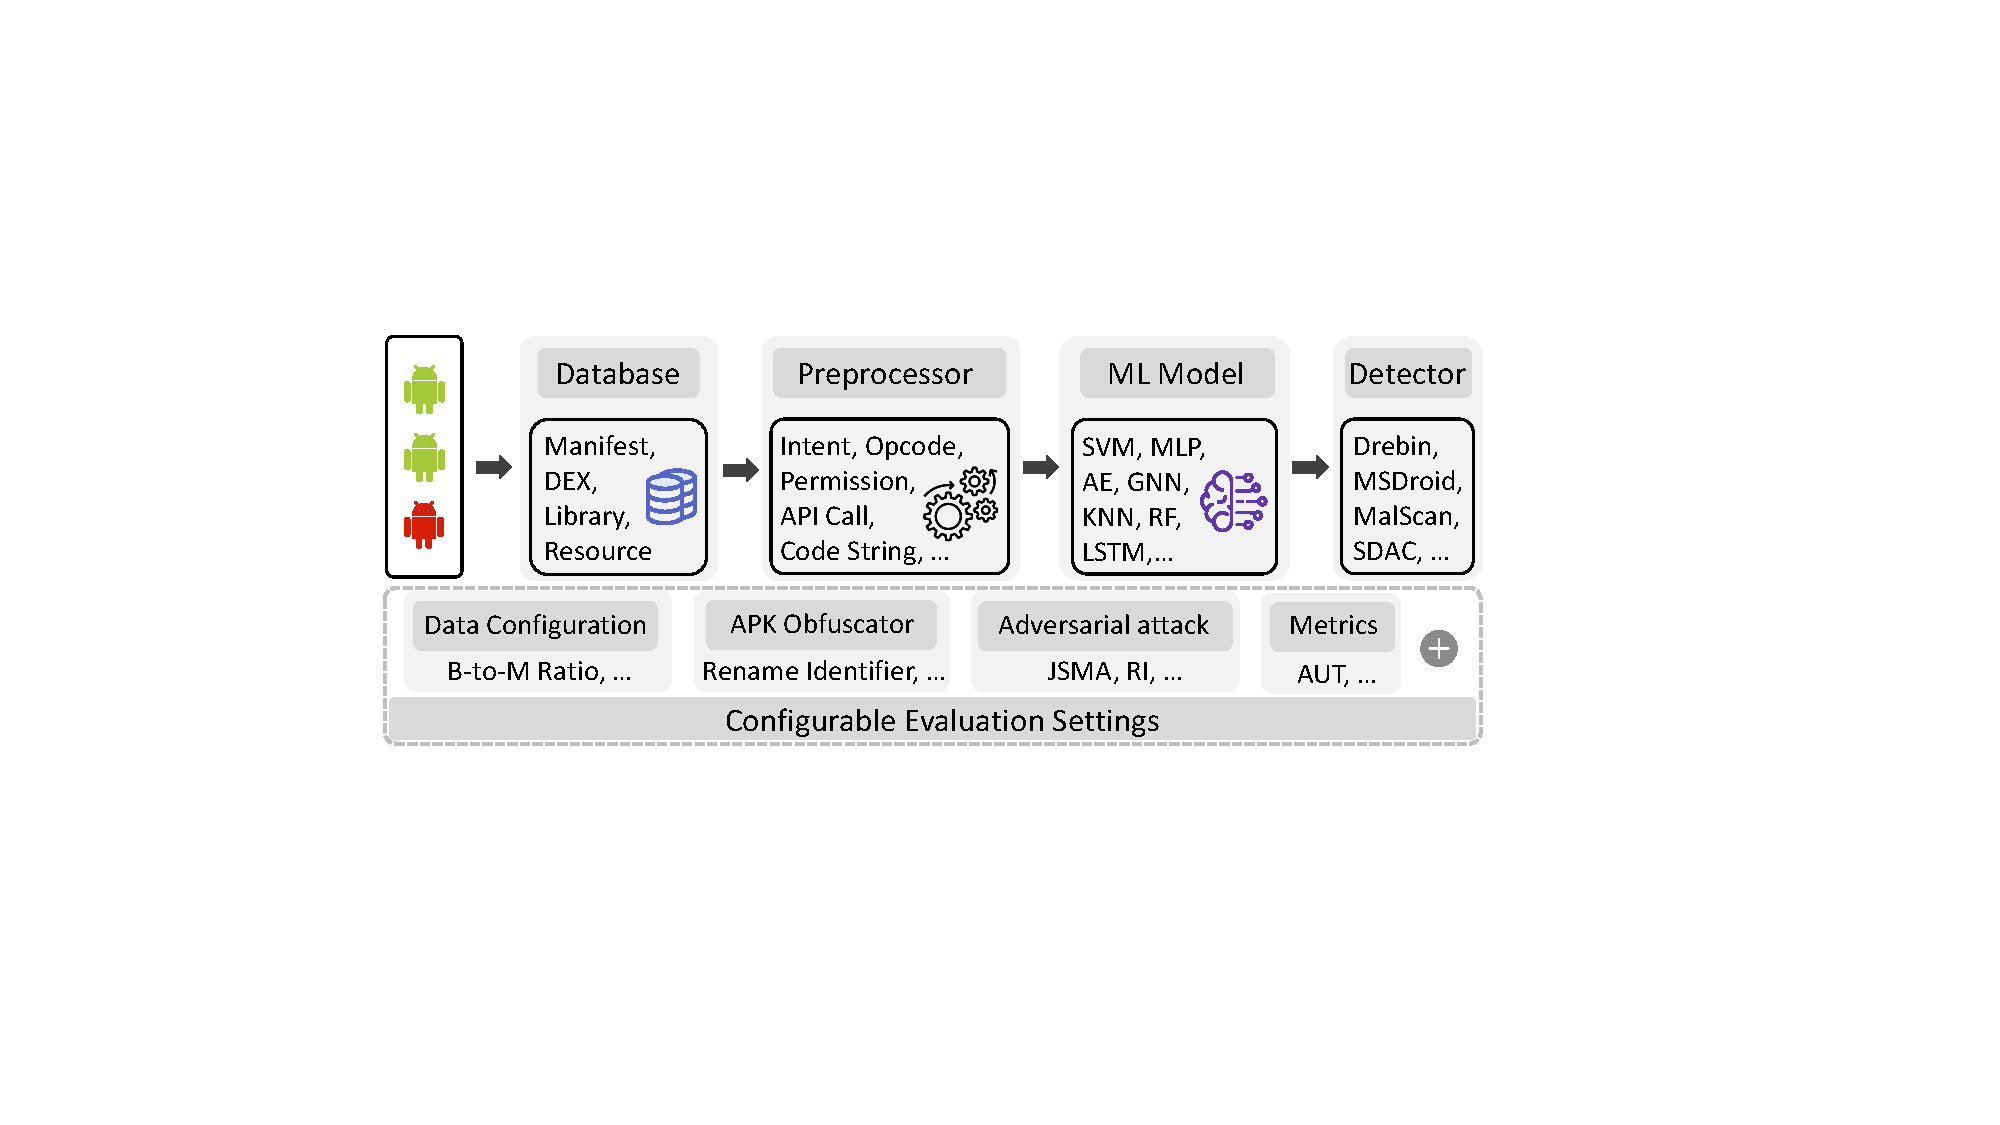
\includegraphics[width=0.84\linewidth]{fig/framework.pdf}
    \DIFaddendFL \vspace{-0.1cm}
    \caption{The \DIFaddbeginFL \DIFaddFL{overall }\DIFaddendFL architecture of \codename.}
    \label{fig:framework}
    \vspace{-0.3cm}
\end{figure}

\DIFdelbegin \DIFdel{Having analyzed existing ML-based Android malware detection approaches}\DIFdelend %DIF >  Having analyzed existing ML-based Android malware detection approaches, we propose a general-purpose framework, \codename, to facilitate the development and evaluation of new Android malware detectors.
\DIFaddbegin 

\DIFadd{To support experimental reproducibility and fair comparison}\DIFaddend , we propose a general-purpose framework, \codename, \DIFaddbegin \DIFadd{guided by the detection workflow discussed in Section~\ref{sec:systematic_investigation}, }\DIFaddend to facilitate the development and evaluation of new Android malware detectors.
Figure~\ref{fig:framework} illustrates the overall architecture and workflow of \codename.
\DIFdelbegin \DIFdel{It starts }\DIFdelend %DIF >  It starts with a collection of apps, from which a set of features is extracted and stored in a {\em feature database}.
\DIFaddbegin \DIFadd{The process begins }\DIFaddend with a collection of apps, from which a set of features is extracted and stored in a {\em feature database}.
These features are then processed by a {\em preprocessor}, \DIFdelbegin \DIFdel{being transformed into a numerical vector.
After that, a }\DIFdelend \DIFaddbegin \DIFadd{which transformes them into numerical vectors.
A }\DIFaddend selected {\em ML model} is \DIFaddbegin \DIFadd{subsequently }\DIFaddend trained and evaluated \DIFdelbegin \DIFdel{for detecting malware.
}\DIFdelend \DIFaddbegin \DIFadd{to detect malicious applications.
Furthermore, }\DIFaddend \codename \DIFdelbegin \DIFdel{is also equipped with adaptable }\DIFdelend \DIFaddbegin \DIFadd{provides configurable }\DIFaddend experimental settings to support \DIFdelbegin \DIFdel{multiple }\DIFdelend \DIFaddbegin \DIFadd{diverse }\DIFaddend real-world scenarios, such as varying goodware-to-malware ratios, \DIFaddbegin \DIFadd{different }\DIFaddend training data sizes, and robustness \DIFaddbegin \DIFadd{assessments }\DIFaddend against adversarial attacks.
% It is implemented in 17K lines of Python code, detailed in Appendix~\ref{sub:implementation}.
%
% The framework is crafted with two guiding principles at its core: modularization and flexibility.
% \jh{\codename is modular, which makes it easy to extend and customize according to various requirements.}
% This is achieved by decoupling it into three modules: \textit{feature database}, \textit{preprocessor}, and \textit{ML model}.
% Given the structured format of the \textit{feature database}, one can easily incorporate new features and integrate them into the assessment pipeline.
% Moreover, the \textit{preprocessor} can be tailored to accommodate various approaches, granting users the flexibility to determine what/how features are used.
% The \textit{ML model} is preloaded with various ML models, such as SVM, MLP, CNN, and AE.
% Alternatively, \codename also supports custom models, allowing users to incorporate their own models into the framework.
% Given the structured format of the \textit{feature database} (details can be found in~\ref{sub:feature_db}), one can easily incorporate new features and integrate them into the assessment pipeline.

This modular design of \codename simplifies the development of ML-based Android malware detectors. Three key modules, \textit{feature database}, \textit{preprocessor}, and \textit{ML model}, captures the main aspects of designing ML solutions for Android malware detection.
% \textit{Feature database} organizes the extracted features categorically, including Manifest, ProgramGraph, DisassembledCode, and SharedLibrary, which can be easily extended to incorporate new features.
\DIFaddbegin \DIFadd{The }\DIFaddend \textit{\DIFdelbegin \DIFdel{Feature }\DIFdelend \DIFaddbegin \DIFadd{feature }\DIFaddend database} organizes \DIFdelbegin \DIFdel{the }\DIFdelend extracted features categorically according to their sources\DIFaddbegin \DIFadd{, }\DIFaddend as discussed in \DIFdelbegin \DIFdel{Sec}\DIFdelend \DIFaddbegin \DIFadd{Section}\DIFaddend ~\ref{sub:apk_characterization}, including Manifest, Dex, Library, and Resource. 
For example, the Manifest category contains features extracted from the AndroidManifest.xml file, such as permissions, intents, and \DIFdelbegin \DIFdel{components.
Details of }\DIFdelend \DIFaddbegin \DIFadd{application components.
Further details about }\DIFaddend the feature database are provided in Appendix~\ref{sub:feature_db}.
\DIFdelbegin \DIFdel{This design allows for easy integration of new features }\DIFdelend \DIFaddbegin \DIFadd{Notably, all features are stored in a manner consistent with our APK characterization taxonomy.
Each directory corresponds to a specific feature source, and the features of a given APK are distributed accordingly --- for instance, Hardware Components and Application Components under Manifest; API Calls, Opcodes, and Program Graphs under Dex; Native Functions under Library; and Image Resources under Resource.
Such structured storage enables developers to easily query and extract the required features without re-extracting them from the original APKs, greatly accelerating the development of new detectors.
%DIF >  For example, users can quickly retrieve a subset of features from the database at the APK characterization level when designing a new detector with \textit{preprocessor}.
In addition, the modular design allows new feature types to be seamlessly integrated }\DIFaddend into the framework.
\DIFaddbegin 

\DIFadd{The }\DIFaddend \textit{\DIFdelbegin \DIFdel{Preprocessor}\DIFdelend \DIFaddbegin \DIFadd{preprocessor}\DIFaddend } \DIFdelbegin \DIFdel{is used to retrieve and encode features before feeding them into }\textit{\DIFdel{ML model}}%DIFAUXCMD
\DIFdelend \DIFaddbegin \DIFadd{retrieves and encodes features before they are fed into the ML model}\DIFaddend .
This module can be \DIFdelbegin \DIFdel{tailored }\DIFdelend \DIFaddbegin \DIFadd{customized }\DIFaddend to support different detectors, \DIFdelbegin \DIFdel{granting }\DIFdelend \DIFaddbegin \DIFadd{providing }\DIFaddend flexibility in feature selection and usage.
\DIFaddbegin \DIFadd{Leveraging the structured organization of the }\textit{\DIFadd{feature database}}\DIFadd{, users can easily select and combine features from multiple sources to construct customized feature vectors.
For instance, when designing a new detector, one can quickly retrieve a subset of features at the APK-characterization level using the }\textit{\DIFadd{preprocessor}}\DIFadd{.
To replicate a detector that relies on API calls and permissions, the }\textit{\DIFadd{preprocessor}} \DIFadd{can be configured to extract these features from the Dex and Manifest categories, respectively, and encode them into a unified feature vector.
}

\DIFadd{The }\DIFaddend \textit{ML model} \DIFdelbegin \DIFdel{integrates widely used ML models, }\textit{\DIFdel{e.g.,}} %DIFAUXCMD
\DIFdelend \DIFaddbegin \DIFadd{module integrates a wide range of commonly used machine learning models, such as }\DIFaddend RF, SVM, KNN, MLP, LSTM, CNN, GNN, and AE.
Each model \DIFdelbegin \DIFdel{provides friendly }\DIFdelend \DIFaddbegin \DIFadd{offers user-friendly }\DIFaddend interfaces for training, testing, and evaluation\DIFdelbegin \DIFdel{.
It also supports model }\DIFdelend \DIFaddbegin \DIFadd{, and the module supports easy }\DIFaddend customization and extension --- for example, \DIFdelbegin \DIFdel{one can easily add new neural networks of different }\DIFdelend \DIFaddbegin \DIFadd{adding new neural network }\DIFaddend architectures.
To develop a new detector, \DIFdelbegin \DIFdel{one only needs to customize }\DIFdelend \DIFaddbegin \DIFadd{users only need to customize the }\DIFaddend \textit{preprocessor} to select \DIFdelbegin \DIFdel{corresponding features from }\DIFdelend \DIFaddbegin \DIFadd{the required features from the }\DIFaddend \textit{feature database} and feed them into \DIFaddbegin \DIFadd{the chosen model within the }\DIFaddend \textit{ML model} \DIFdelbegin \DIFdel{.
If no required features and models are available, users can easily extend the framework }\DIFdelend \DIFaddbegin \DIFadd{module.
If certain features or models are not yet supported, the framework can be readily extended }\DIFaddend by adding new \DIFdelbegin \DIFdel{features }\DIFdelend \DIFaddbegin \DIFadd{feature types }\DIFaddend to the \textit{feature database} and \DIFdelbegin \DIFdel{new learning models to the }\textit{\DIFdel{ML model}} %DIFAUXCMD
\DIFdelend \DIFaddbegin \DIFadd{incorporating additional learning models into the ML }\DIFaddend module.


\codename provides configurable experimental settings to support different \DIFaddbegin \DIFadd{evaluation }\DIFaddend scenarios.
Parameters, such as\DIFaddbegin \DIFadd{, training sample size, }\DIFaddend goodware-to-malware ratios, \DIFdelbegin \DIFdel{sample time distribution , and training data sizes, }\DIFdelend \DIFaddbegin \DIFadd{and temporal distribution of samples, }\DIFaddend are all adjustable.
\DIFdelbegin \DIFdel{This }\DIFdelend \DIFaddbegin \DIFadd{The framework offers fine-grained control over these parameters and supports checkpointing during both training and evaluation.
This flexibility }\DIFaddend facilitates app selection \DIFdelbegin \DIFdel{to construct diverse scenarios}\DIFdelend \DIFaddbegin \DIFadd{and scenario construction}\DIFaddend , ensuring comprehensive and accurate \DIFdelbegin \DIFdel{evaluation.
For instance, one }\DIFdelend \DIFaddbegin \DIFadd{evaluations.
For example, users }\DIFaddend can configure the \DIFdelbegin \DIFdel{ratio of }\DIFdelend goodware-to-malware \DIFdelbegin \DIFdel{to evaluate the model 's performance under different }\DIFdelend \DIFaddbegin \DIFadd{ratio to assess model performance under varying }\DIFaddend malware prevalence.
\DIFdelbegin \DIFdel{We can adjust the apps distribution over time to simulate the evolution of malware }\DIFdelend \DIFaddbegin \DIFadd{They can also adjust the temporal distribution of apps to simulate malware evolution}\DIFaddend , which is \DIFdelbegin \DIFdel{crucial for assessing the model 's robustness.
}\DIFdelend \DIFaddbegin \DIFadd{essential for evaluating model robustness.
Furthermore, with flexible training-sample configuration and organized checkpoint management, }\DIFaddend \codename \DIFdelbegin \DIFdel{also includes }\DIFdelend \DIFaddbegin \DIFadd{enables incremental training, allowing users to incorporate new training samples and continue training from existing models.
}

%DIF >  \codename offers fine-grained control over these parameters and support checkpointing during training and evaluation.
%DIF >  This facilitates app selection to construct diverse scenarios, ensuring comprehensive and accurate evaluation.
%DIF >  For instance, one can configure the ratio of goodware-to-malware to evaluate the model's performance under different malware prevalence.
%DIF >  We can adjust the apps distribution over time to simulate the evolution of malware, which is crucial for assessing the model's robustness.
%DIF >  Given the flexibility to adjust training samples and categorize model checkpoints, \codename also enables incremental training, allowing users to add new training samples and continue training from existing models. 

\codename \DIFadd{also integrates }\DIFaddend an APK obfuscator~\cite{aonzo2020obfuscapk}, which can produce \DIFdelbegin \DIFdel{different }\DIFdelend \DIFaddbegin \DIFadd{various }\DIFaddend types of obfuscated samples, \textit{e.g.\DIFdelbegin \DIFdel{,}\DIFdelend }\DIFaddbegin \DIFadd{, }\DIFaddend identifier renaming, resource encryption, code modification, and invocation reflection.
\DIFdelbegin \DIFdel{This feature }\DIFdelend \DIFaddbegin \DIFadd{Obfuscation is applied to APKs before feature extraction to generate their obfuscated variants.
The different obfuscation types can be applied as independent operations: one can first apply one type of obfuscation and then apply another to an already obfuscated APK. 
This capability }\DIFaddend is essential for evaluating the model's resilience to obfuscated malware.
Moreover, this framework incorporates an adversarial \DIFdelbegin \DIFdel{samples }\DIFdelend \DIFaddbegin \DIFadd{sample }\DIFaddend generation mechanism from AndroidHIV~\cite{chen2019android}, \DIFdelbegin \DIFdel{allowing }\DIFdelend \DIFaddbegin \DIFadd{enabling }\DIFaddend the assessment of \DIFdelbegin \DIFdel{models' }\DIFdelend \DIFaddbegin \DIFadd{model }\DIFaddend resilience to adversarial attacks.
\DIFaddbegin \DIFadd{Specifically, adversarial samples are generated by perturbing the feature vectors of original samples, and these perturbed samples are then used to evaluate the robustness of the trained models.
The perturbation process ensures that the functionality of the original apps is preserved.
Further details can be found in AndroidHIV~\mbox{%DIFAUXCMD
\cite{chen2019android}}\hskip0pt%DIFAUXCMD
.
}\DIFaddend Such flexibility and adaptability make \codename a versatile tool for developing and evaluating ML-based Android malware detectors.
\DIFaddbegin 


%DIF >  \tosem{Add discussion about the training methods, such as incremental training, only need to add new training samples, and load existing models for further traning.
%DIF >  As for the obfuscation techniques, our framework re-parses the apks, can support the concurrently, if applying them to the apks.}



\DIFaddend % The implementation of \codename is in the Appendix~\ref{sub:implementation}.


% \bulletpoint{\codename Implementation}
% \codename is developed in 17K lines of Python code.
% To ensure consistency and mitigate biases from different feature extraction toolchains and learning frameworks, we adopt standardized techniques across all tasks.
% For feature extraction, we use Androguard~\cite{androguard} to disassemble APK files and derive features such as permissions, intents, and program graphs. 
% LibRadar~\cite{libradar} helps in identifying third-party libraries within the applications, while Angr~\cite{angr} is used for analyzing native libraries and capturing essential features like opcodes and API calls. 
% When it comes to ML models, the scikit-learn library is our choice for traditional ML algorithms like SVM, KNN, and RF.
% On the other hand, for DL architectures such as CNN, GNN, and AE, we resort to Pytorch~\cite{pytorch}.
% This uniform approach ensures a balanced evaluation, concentrating purely on the uniqueness and performance of each method.

\bulletpoint{\codename Implementation}
\codename is developed in 17K lines of Python code.
To ensure consistency and mitigate biases from different feature extraction toolchains and learning frameworks, we adopt \DIFdelbegin \DIFdel{standardized techniques across all tasks}\DIFdelend \DIFaddbegin \DIFadd{a standardized setup across all Android malware detectors}\DIFaddend .
For feature extraction, we use Androguard~\cite{androguard} to disassemble APK files and derive features such as permissions, intents, and program graphs. 
LibRadar~\cite{libradar} helps in identifying third-party libraries within the applications, while Angr~\cite{angr} is used for analyzing native libraries and capturing essential features like opcodes and API calls. 
When it comes to \DIFdelbegin \DIFdel{ML }\DIFdelend \DIFaddbegin \DIFadd{machine learning }\DIFaddend models, the scikit-learn library is our choice for traditional ML algorithms like SVM, KNN, \DIFaddbegin \DIFadd{DT }\DIFaddend and RF.
On the other hand, for \DIFdelbegin \DIFdel{DL }\DIFdelend \DIFaddbegin \DIFadd{deep learning }\DIFaddend architectures such as CNN, GNN, and AE, we resort to Pytorch~\cite{pytorch}.
This uniform approach ensures a balanced evaluation, concentrating purely on the uniqueness and performance of each method.
\DIFdelbegin \DIFdel{We will make }\DIFdelend \DIFaddbegin 

\bulletpoint{Potential usage and availability of \codename}
\DIFadd{As discussed above, }\DIFaddend \codename \DIFdelbegin \DIFdel{publicly available to the research community to facilitate }\DIFdelend \DIFaddbegin \DIFadd{is designed with a modular and flexible architecture, making it easy to extend and customize to meet diverse research and evaluation requirements.
The framework also incorporates a comprehensive app dataset that spans a wide range of Android applications across different time periods.
Researchers and practitioners can readily leverage }\codename \DIFadd{to develop new ML-based Android malware detectors, evaluate their performance under diverse scenarios, and compare them with existing approaches in a fair and consistent manner.
For example, when designing a new detector based on API calls and permissions, users can easily retrieve these features from the }\textit{\DIFadd{feature database}} \DIFadd{and feed them into their proposed model for evaluation.
Likewise, existing detectors can be readily reproduced by appropriately configuring the }\textit{\DIFadd{preprocessor}} \DIFadd{and selecting the corresponding models from the }\textit{\DIFadd{ML model}} \DIFadd{module, enabling systematic and reproducible comparisons.
}


\DIFadd{Currently, }\codename \DIFadd{is available to interested researchers upon request.
It has already been adopted by several academic and industrial organizations across multiple countries, including the United States, Germany, Singapore, and China, for the development and evaluation of ML-based Android malware detectors.
This level of adoption demonstrates the practicality and effectiveness of }\codename \DIFadd{in supporting malware analysis research.
We plan to release }\codename \DIFadd{publicly to further facilitate and accelerate }\DIFaddend future research in this \DIFdelbegin \DIFdel{area}\DIFdelend \DIFaddbegin \DIFadd{domain}\DIFaddend .
\vspace{-0.1cm}
\section{Representative Approach Analysis}
\label{sec:approach_analysis}

% To understand the state of ML-based Android malware detection, a quantitative analysis of current work is indispensable.

% With the rapid evolution of this field, hundreds of techniques have been proposed and achieved remarkable performance in the past decade.
% A systematic investigation of relevant works dating back to 2011 is discussed in Sec.~\ref{sec:discussion} to highlight extensive efforts that have been devoted to Android malware detection.

% While an ideal scenario is evaluating as many approaches as possible, conducting an exhaustive examination of each method is impractical due to the vast amount of existing literature.

% Moreover, it is important to know that, despite the abundance of publications in this area, many papers present slight variations of similar techniques, and novel solutions are comparatively fewer.
% Moreover, it is important to understand that, despite vast publications in this area achieving promising results, many of them share similar techniques (\textit{e.g.,} similar neural networks), and novel solutions are comparatively fewer.

% Thus, our analysis focuses on methods that represent the broad spectrum and depth of advancements in the field.
% In the section, we first outline the selection principles and provide a summary of the selected approaches.
% Then, a comparative analysis is presented to offer insights into the experimental designs.

To understand the state of ML-based Android malware detection, a quantitative analysis of current work is indispensable.
While an ideal scenario is evaluating as many approaches as possible, conducting an exhaustive examination of each method is impractical due to the vast amount of existing literature.
\DIFaddbegin \DIFadd{Moreover, it is important to understand that, despite vast publications in this area achieving promising results, many of them share similar techniques (}\textit{\DIFadd{e.g.,}} \DIFadd{similar neural networks), and novel solutions are comparatively fewer.
}\DIFaddend Thus, our analysis focuses on methods that represent the broad spectrum and depth of advancements in the field.
That is, we aim to select representative approaches and utilize our framework to re-implement and evaluate them.
Specifically, in this section, we outline the selected approaches and provide a comparative analysis to highlight their experimental designs.
We then quantitatively evaluate these approaches in \DIFdelbegin \DIFdel{Sec.}\DIFdelend \DIFaddbegin \DIFadd{Section}\DIFaddend ~\ref{sec:evaluation}, shedding further light on the current state of ML-based Android malware detection.

% In the section, we first outline the selection principles and provide a summary of the selected approaches.
% Then, a comparative analysis is presented to offer insights into the experimental designs.

\subsection{Selection Criteria}
\label{sub:selection_criteria}

\bulletpoint{Cover various communities}
Android malware detection stands as an interdisciplinary domain, drawing contributions from diverse communities, including software engineering, security, and machine learning.
However, a notable separation is observed --- the solutions in one community often only compare with others from the same community --- which hinders potential collaborative advancements.
For instance, methods like~\cite{hou2017hindroid,ye2019out} from one community are often evaluated in isolation, complicating direct performance comparison.
To bridge the gap, we incorporate approaches from leading venues across a broad range of communities.
% To address this, we select approaches from a range of communities.

% This includes various mixes of APK features, feature representations, and ML models.
\bulletpoint{Explore an extensive spectrum of techniques in the detection pipeline}
As identified in Sec.~\ref{sec:systematic_investigation}, a wide range of technique combinations exists across different phases of the detection pipeline.
This study explores as many techniques as possible in each phase, including various mixes of APK features, feature representations, and ML models.
Such a comprehensive investigation enables us to gain a thorough understanding of the entire workflow of ML-based Android malware detection.

% \jh{This study explores these stages, examining various mixes of APK features, feature representations, and ML models.
% Such a comprehensive investigation enables us to gain a thorough understanding of the entire workflow of Android malware detection.}

\bulletpoint{Reflect research progress}
\DIFdelbegin \DIFdel{Considering the evolving landscape of this field, where novel methods }\DIFdelend %DIF >  Considering the evolving landscape of this field, where novel methods continually emerge, we prioritize approaches that introduce new techniques or achieve remarkable performance, such as proposing new feature representations or employing new learning architectures.
\DIFaddbegin \DIFadd{In consideration of the evolving research landscape, where new methodologies }\DIFaddend continually emerge, we \DIFdelbegin \DIFdel{prioritize }\DIFdelend \DIFaddbegin \DIFadd{place emphasis on }\DIFaddend approaches that introduce \DIFdelbegin \DIFdel{new techniquesor achieve remarkable performance, such as proposing new }\DIFdelend \DIFaddbegin \DIFadd{cutting-edge techniques.
Particularly, we prioritize methods that either propose novel }\DIFaddend feature representations or \DIFdelbegin \DIFdel{employing new learning architectures.
%DIF <  In consideration of the evolving research landscape, where new methodologies continually emerge, we place emphasis on approaches that introduce cutting-edge techniques.
}\DIFdelend \DIFaddbegin \DIFadd{employ innovative learning architectures, or achieve remarkable performance in the field.
}\DIFaddend 

% Given the dynamic nature of the research landscape where novel methodologies emerge, and existing ones are refined, \jh{we prioritize approaches that introduce novel techniques such as employing a new learning architecture or proposing a new feature representation, or achieve remarkable performance in the field.}

% Particularly, our attention is centered on approaches that either introduce novel techniques or achieve remarkable performance in the field.
% A case in point is MsDroid~\cite{he2022msdroid}, representing the forefront of GNN-based Android malware detection.

\bulletpoint{Emphasize representative approaches over specific papers}
% Recognizing that some approaches are either variants or amalgamations of existing ones, we concentrate our efforts on examining representative strategies.
% Numerous studies propose variations of existing approaches, often achieving similar performance to the original approaches.
% \jh{Analyzing these approaches would be redundant and uninformative.}
% \jh{Therefore, our analysis is specifically oriented towards distinct and representative strategies.}
%
% \jh{Numerous studies are variants or combinations of existing methods, typically yielding similar performance to the original approaches.
% Analyzing these derivative approaches could lead to redundancy and provide limited insights.
% Therefore, our analysis is deliberately focused on distinct and representative strategies that offer more significant contributions to this field.}
%
Many approaches share similar techniques, extracting patterns from analogous feature sets (\textit{e.g.,} program graphs) with similar ML models such as different variants of GNNs.
Analyzing these methods could lead to redundancy and provide limited insights.
Thus, we focus on distinct and representative strategies that offer more significant contributions.

% We recognize that some methods in the field are variants or amalgamations of existing approaches. 
% To steer clear of redundancy, we have curated a list of distinct and representative approaches.


\begin{table*}[t]
  \centering
  % \renewcommand{\arraystretch}{0.88}
  \caption{A summary of our selected approaches regarding APK Characterization, Feature Representation, and ML Models.
  \ymark \ indicates that the APK feature is utilized in feature engineering, while \nmark \ is the opposite.}
  \DIFdelbeginFL %DIFDELCMD < \vspace{-0.1cm}
%DIFDELCMD <   %%%
\DIFdelendFL \DIFaddbeginFL \vspace{-0.2cm}
  \DIFaddendFL \begin{adjustbox}{width=\linewidth, center}
  \begin{tabular}{@{}c|cccccccccc|c|cc@{}}
  \toprule
  \multirow{2}{*}{\textbf{\begin{tabular}[c]{@{}c@{}}\\Selected \\ Approach\end{tabular}}} & \multicolumn{10}{c|}{\textbf{APK Characterization}} & \multirow{2}{*}{\textbf{\begin{tabular}[c]{@{}c@{}} \\Feature \\ Representation\end{tabular}}} & \multirow{2}{*}{\textbf{\begin{tabular}[c]{@{}c@{}} \\ML \\ Models\end{tabular}}} \\ \cmidrule(lr){2-11}
    &\textbf{\begin{tabular}[c]{@{}c@{}}Hardware\\ Component\end{tabular}} & \textbf{\begin{tabular}[c]{@{}c@{}}Application\\ Component\end{tabular}} & \textbf{Intent} & \textbf{Permission} & \textbf{\begin{tabular}[c]{@{}c@{}}API\\ Call\end{tabular}} & \textbf{\begin{tabular}[c]{@{}c@{}}Byte\\ Code\end{tabular}} & \textbf{Opcode} & \textbf{\begin{tabular}[c]{@{}c@{}}Code\\ String\end{tabular}} & \textbf{\begin{tabular}[c]{@{}c@{}}Program\\ Graph\end{tabular}} & \textbf{\begin{tabular}[c]{@{}c@{}}Resource\\ Information\end{tabular}} &   \\ \midrule

  Drebin~\cite{arp2014drebin}&\ymark&\ymark&\ymark&\ymark&\ymark&\nmark&\nmark&\ymark&\nmark&\nmark& Categorical & SVM &  \\ \midrule
  MamaDroid~\cite{mariconti2016mamadroid} &\nmark&\nmark&\nmark&\nmark&\ymark&\nmark&\nmark&\nmark&\ymark&\nmark& Graph-based & RF &  \\ \midrule
  Mclaughlin et al.~\cite{mclaughlin2017deep} &\nmark&\nmark&\nmark&\nmark&\nmark&\nmark&\ymark&\nmark&\nmark&\nmark& Image-based & CNN  \\ \midrule
  HinDroid~\cite{hou2017hindroid} &\nmark&\nmark&\nmark&\nmark&\ymark&\nmark&\nmark&\nmark&\ymark&\nmark& Graph-based & SVM  \\ \midrule
  DeepRefiner~\cite{xu2018deeprefiner}  &\ymark&\ymark&\ymark&\ymark&\nmark&\ymark&\nmark&\nmark&\nmark&\ymark& Text-based & LSTM  \\ \midrule
  Kim et al.~\cite{kim2018multimodal} &\ymark&\ymark&\ymark&\ymark&\ymark&\nmark&\ymark&\ymark&\nmark&\nmark& Categorical & MLP   \\ \midrule
  MalScan~\cite{wu2019malscan} &\nmark&\nmark&\nmark&\nmark&\ymark&\nmark&\nmark&\nmark&\ymark&\nmark& Graph-based & KNN   \\ \midrule
  SDAC~\cite{xu2020sdac} &\nmark&\nmark&\nmark&\nmark&\ymark&\nmark&\nmark&\nmark&\ymark&\nmark& Categorical & SVM   \\ \midrule
  HomDroid~\cite{wu2021homdroid} &\nmark&\nmark&\nmark&\nmark&\ymark&\nmark&\nmark&\nmark&\ymark&\nmark& Categorical & KNN & \\ \midrule
  Xmal~\cite{wu2021android} &\nmark&\nmark&\nmark&\ymark&\ymark&\nmark&\nmark&\nmark&\nmark&\nmark& Categorical & MLP  \\ \midrule
  RAMDA~\cite{li2021robust} &\nmark&\nmark&\ymark&\ymark&\ymark&\nmark&\nmark&\nmark&\nmark&\nmark& Categorical & AE  \\ \midrule
  MSDroid~\cite{he2022msdroid} &\nmark&\nmark&\nmark&\ymark&\ymark&\nmark&\ymark&\ymark&\ymark&\nmark& Graph-based & GNN  \\ \bottomrule
  \end{tabular}
  \end{adjustbox}

  \centering
  \label{tbl:systematization}
  \begin{tablenotes}
  \footnotesize
  \item While multiple ML models may be utilized in individual approaches~\cite{mariconti2016mamadroid,wu2019malscan,wu2021homdroid}, we only report the model that yields the best effectiveness (\textit{e.g.}, F1-score).
  \end{tablenotes}
  \label{tab:apk_characterization}
  \DIFdelbeginFL %DIFDELCMD < \vspace{-0.5cm}
%DIFDELCMD < %%%
\DIFdelendFL \DIFaddbeginFL \vspace{-0.4cm}
\DIFaddendFL \end{table*}

\subsection{Selected Approaches}
\label{sub:selected_approaches}

In \DIFdelbegin \DIFdel{Sec}\DIFdelend \DIFaddbegin \DIFadd{Section}\DIFaddend ~\ref{sec:systematic_investigation} we have presented recent advancements in ML-based Android malware detection, by dissecting the detection pipeline into three phases: APK characterization, feature representation, and ML modeling.
Adhering to the selection criteria, we identify 12 representative approaches from hundreds of available solutions to analyze the current state of this field.
During the selection process, to foster collaboration among different fields, we prioritize the approaches published in leading venues from three communities, such as ASE, TOSEM from software engineering, NDSS, TIFS from security, and KDD, WWW from machine learning.
Specifically, the selected approaches include 3 from software engineering, 7 from security, and 2 from machine learning.
A detailed summary about sources and publication years of these approaches is provided in Table~\ref{tab:literature}.
We also ensure that the selected approaches cover almost all the APK characterization, feature representation, and ML models discussed in \DIFdelbegin \DIFdel{Sec.}\DIFdelend \DIFaddbegin \DIFadd{Section}\DIFaddend ~\ref{sec:systematic_investigation}.
As Table~\ref{tab:apk_characterization} shows, they are carefully chosen to represent a broad range of techniques employed in the detection process, including 10 APK features, 4 feature representations, and 8 ML models.
Additionally, the selected approaches are distinguished either by their promising performance or by introducing novel techniques.
For instance, both MsDroid~\cite{he2022msdroid} and EFCG~\cite{cai2021learning} are recent works that introduce GNNs to detect malicious patterns in APKs.
We highlight MsDroid as it better represents apps' graph structures via aggregating more channel information and currently stands as the state-of-the-art in Android malware detection using GNNs.
Importantly, we also make a concerted effort to ensure that the selected solutions are not variants of existing ones.
For example, several methods~\cite{hou2017hindroid,ye2019out,fan2021heterogeneous} utilize heterogeneous graphs to model APKs, we select HinDroid~\cite{hou2017hindroid} because it introduces a novel feature representation that encodes diverse API call relationships while achieving performance comparable to other methods.
To better understand the selected representative approaches, we introduce them in the following section.
% Adhering to the selection criteria, we identify 12 representative approaches from hundreds of available solutions to analyze the current state of ML-based Android malware detection.
% These methods are carefully chosen from 3 communities --- security, software engineering, and machine learning.
% This selection guarantees a broad range of techniques employed in the detection process, including 10 APK features, 4 feature representations, and 8 ML models.
% Importantly, the selected approaches stand out either by demonstrating promising performance or bringing novel techniques, \textit{e.g.}, GNN~\cite{he2022msdroid} and CNN~\cite{mclaughlin2017deep}.
% Additionally, we have made a concerted effort to ensure that the selected solutions are not variants of existing ones.
% For instance, while several methods~\cite{hou2017hindroid,ye2019out,fan2021heterogeneous} utilize heterogeneous information graphs to model APKs, we spotlight the pioneering approach~\cite{hou2017hindroid} that first introduces this concept.
% \jh{In the remaining section, we introduce these approaches.}
% integrating the information presented in Table~\ref{tab:apk_characterization}.


% In our exploration, we tap into the major venues from diverse communities (\textit{i.e.,} security, software engineering, and machine learning) to identify representative approaches.
% We cover almost all the APK characterization, feature representation, and ML models discussed in Section~\ref{sec:systematic_investigation}.
% We prioritize state-of-the-art approaches that introduce novel techniques to the field, such as GNN~\cite{he2022msdroid} and CNN~\cite{mclaughlin2017deep}.
% Also, when selecting, we exclude approaches that are variants or combinations of existing ones.
% For instance, while several methods~\cite{hou2017hindroid,ye2019out,fan2021heterogeneous} utilize heterogeneous information graphs to model APKs, we spotlight the pioneering approach~\cite{hou2017hindroid} that first introduced this concept in Android malware detection.

% Based on this selection process, we have identified 12 representative approaches, which are summarized in Table~\ref{tab:literature}.
% We now introduce the selected approaches, combining with the information presented in Table~\ref{tab:apk_characterization}.

\bulletpoint{Drebin}
% The approach presented in~\cite{arp2014drebin} serves as a foundational work in ML-based Android malware detection.
% Through static analysis, it collects features from APKs, such as hardware components, intents, and API calls.
Drebin~\cite{arp2014drebin} first collects APK features, such as hardware components, permissions, intents, and API calls, using static analysis.
These features are then converted into a binary vector to signify their existence or not.
An SVM is then trained to detect Android malware.

%DIF >  \jh{With the Markov chain constructed from API call sequences, the transition probabilities between these calls are computed as features.}
\bulletpoint{MamaDroid}
MamaDroid~\cite{mariconti2016mamadroid} pioneers the use of Markov chains to \DIFdelbegin \DIFdel{depict apps' behaviors. 
}%DIFDELCMD < \jh{With the Markov chain constructed from API call sequences, the transition probabilities between these calls are computed as features.}
%DIFDELCMD < %%%
%DIF <  By constructing a Markov chain based on the sequence of abstracted API calls invoked by an app, the transition probabilities between these calls are computed as features. 
%DIFDELCMD < \jh{These features then inform an RF model to detect Android malware.}
%DIFDELCMD < %%%
\DIFdelend \DIFaddbegin \DIFadd{model app behavior. 
It constructs a Markov chain over the sequence of abstracted API calls invoked by an app and computes the transition probabilities between these calls as features, which are then used by an RF classifier to detect Android malware.
}\DIFaddend 

\bulletpoint{Mclaughlin et al}
This technique~\cite{mclaughlin2017deep} presents the leading edge in image-based Android malware detection.
By transforming opcode sequences into images via a one-hot encoding, it leverages a CNN model to classify them as benign or malicious samples.
% \jh{By transforming opcode sequences into images via one-hot encoding, it leverages a CNN model to distinguish malware.}

\bulletpoint{HinDroid}
Hou et al.~\cite{hou2017hindroid} introduce a novel approach by representing API calls as a structured heterogeneous information graph.
This approach accounts for the inter-relationships among API calls, such as their presence in the same code block.
It then captures apps' semantics with meta-path techniques\DIFdelbegin %DIFDELCMD < [%%%
\DIFdel{89}%DIFDELCMD < ]%%%
\DIFdelend \DIFaddbegin \DIFadd{~\mbox{%DIFAUXCMD
\cite{sun2011pathsim}}\hskip0pt%DIFAUXCMD
}\DIFaddend .
A multi-kernel SVM is further applied to recognize malicious patterns.


% Hou et al.~\cite{hou2017hindroid} represent API calls as a structured heterogeneous information graph, and then capture apps' semantics with meta-path techniques~\cite{sun2011pathsim}.
% W meta-path techniques~\cite{sun2011pathsim}, it captures the deeper semantics of apps.
% A multi-kernel SVM is further applied to recognize malicious patterns.
% This approach accounts for the inter-relationships among API calls, such as their presence in the same code block.

\bulletpoint{DeepRefiner}
DeepRefiner~\cite{xu2018deeprefiner} designs a two-layer malware detection system.
Initially, it feeds features like hardware components, permissions, and resources into an MLP to detect most malware.
For ambiguous cases, it further interprets APK bytecodes as text sequences and employs an LSTM model to capture the method-level and application-level semantics behind app behaviors.

\bulletpoint{Kim et al}
Kim et al.~\cite{kim2018multimodal} use multi-modal learning to detect malware, aggregating various features, such as intent and API calls. 
Distinct MLPs are initially utilized to process individual features independently. 
Subsequently, a unified MLP integrates the outputs from the preceding models, offering a consolidated decision on malware identification.

\bulletpoint{MalScan}
This study~\cite{wu2019malscan} treats program graphs as social networks, where API calls are treated as nodes, and the relationships between them are presented as edges.
The system further evaluates the centrality of sensitive API calls in the graph to derive features and then feeds them into a KNN model to detect malware.

\bulletpoint{SDAC}
\jh{It attempts to cluster API calls based on their contextual information extracted from API call sequences~\cite{xu2020sdac}.}
These resulting clusters act as features to represent APKs. 
An SVM model is then used to capture malicious patterns.

\bulletpoint{HomDroid}
The method~\cite{wu2021homdroid} focuses on suspicious parts of malware by calculating the homophily in its program graph.
%  paving a novel path for malware detection.
From the malicious subgraphs, it derives two key features: (1) the presence of sensitive API calls, and (2) the number of sensitive triads. 
\jh{These features are then fed into a KNN model to detect malware.}

\bulletpoint{Xmal}
% Given extracted API calls and permissions, Xmal~\cite{wu2021android} introduces an attention-based MLP to differentiate malware from benign apps.
Xmal~\cite{wu2021android} utilizes MLPs to distill information from extracted API calls and permissions for Android malware detection.
It further integrates an attention mechanism to highlight the most informative features.
This attention-based MLP not only achieves promising results but also offers an interpretation of the model.

\bulletpoint{RAMDA}
This detector~\cite{li2021robust} is the SOTA approach that employs Autoencoder to derive a resilient representation of APKs with features such as API calls and intents.
The representation is fed into an MLP to detect malware.

\bulletpoint{MSDroid}
MSDroid~\cite{he2022msdroid} is the cutting-edge in utilizing GNN to detect malware.
Initially, it breaks down the program graph into subgraphs rooted at sensitive API calls. 
Then, it leverages a GNN to capture essential semantics from the graph representations for malware detection.

% \vspace{-0.2cm}
\subsection{Comparative Study}
\label{sub:compare}

\begin{table*}[t]
  \centering
  % \renewcommand{\arraystretch}{0.94}
  \caption{A comparative study of our selected approaches based on their experimental setup, efficiency evaluation, robustness evaluation, artifact release, and toolchain. 
  --- denotes the absence of the statistics in the literature. 
  \ymark \ indicates that both feature encoding and ML modeling were evaluated for efficiency, \halfmark \ indicates that only ML modeling was evaluated, and \nmark \ indicates that the efficiency was not evaluated. 
  Malware Ratio refers to the proportion of malware samples in a testing set.}
  \vspace{-0.1cm}
  \begin{adjustbox}{width=\linewidth, center}

  \begin{tabular}{@{}c|rccc|c|ccc|c|c@{}}
  \toprule
  \multirow{2}{*}{\textbf{\begin{tabular}[c]{@{}c@{}}\\Selected \\ Approach\end{tabular}}} & \multicolumn{4}{c|}{\textbf{Experimental Setup}} & \multirow{2}{*}{\textbf{\begin{tabular}[c]{@{}c@{}}\\Efficiency\\Evaluation\end{tabular}}} & \multicolumn{3}{c|}{\textbf{Robustness Evaluation}} & \multirow{2}{*}{\textbf{\begin{tabular}[c]{@{}c@{}}\\Artifact \\ Release\end{tabular}}} & \multirow{2}{*}{\textbf{\begin{tabular}[c]{@{}c@{}}\\Tool \\ Chain\end{tabular}}} \\ \cmidrule(lr){2-5} \cmidrule(lr){7-9}
   & \textbf{\begin{tabular}[c]{@{}c@{}}Dataset \\ Size\end{tabular}} & \textbf{\begin{tabular}[c]{@{}c@{}}Time \\ Span\end{tabular}} & \textbf{\begin{tabular}[c]{@{}c@{}}Train:\\ Val:Test\end{tabular}} & \textbf{\begin{tabular}[c]{@{}c@{}}Malware\\Ratio\end{tabular}} &  & \textbf{Evolution} & \textbf{Obfuscation} & \textbf{\begin{tabular}[c]{@{}c@{}}Adversarial\\ Sample\end{tabular}} &  \\ \midrule
  Drebin~\cite{arp2014drebin} & 129,013 & 2010-2012 & 2:0:1 & 4\% & \ymark & \xmark & \xmark & \xmark & \cmark & Androguard \\ \midrule
  % ICCDetector~\cite{xu2016iccdetector} & 17,290 & 2010-2012, 2014 & 9:0:1 & 33\% & \ymark & \xmark & \xmark & \xmark & \xmark \\ \midrule
  MamaDroid~\cite{mariconti2016mamadroid} & 43,940 & 2010-2016 & 9:0:1 & 50\% & \ymark & \cmark & \xmark & \xmark & \cmark &Soot\\ \midrule
  Mclaughlin et al.~\cite{mclaughlin2017deep} & 27,395 & --- & --- & 50\% & \halfmark & \xmark & \xmark & \xmark & \cmark & BackSmali \\ \midrule
  HinDroid~\cite{hou2017hindroid} & 2,334 & 2017-2017 & 4:0:1 & 60\% & \halfmark & \xmark & \xmark & \xmark & \xmark & APKTool\\ \midrule
  DeepRefiner~\cite{xu2018deeprefiner} & 110,440 & --- & \textbf{8:1:1} & 57\% & \ymark & \xmark & \cmark & \cmark & \xmark & APKTool\\ \midrule
  Kim et al.~\cite{kim2018multimodal} & 41,260 & --- & \textbf{3:1:1} & 50\% & \halfmark & \xmark & \cmark & \xmark & \xmark & APKTool\\ \midrule
  MalScan~\cite{wu2019malscan} & 30,715 & 2011-2018 & 9:0:1 & 50\% & \ymark & \cmark & \xmark & \cmark & \cmark & Androguard\\ \midrule
  SDAC~\cite{xu2020sdac} & 70,142 & 2011-2016 & 8:0:2 & 50\% & \ymark & \cmark & \cmark & \xmark & \xmark & FlowDroid\\ \midrule
  HomDroid~\cite{wu2021homdroid} & 8,198 & --- & 9:0:1 & 40\% & \ymark & \xmark & \xmark & \xmark & \xmark & Androguard\\ \midrule
  Xmal~\cite{wu2021android} & 35,690 & --- & 7:0:3 & 43\% & \nmark & \xmark & \xmark & \xmark & \cmark & Androguard\\ \midrule
  RAMDA~\cite{li2021robust} & 58,483 & --- & 19:0:1 & 50\% & \nmark & \xmark & \xmark & \cmark & \cmark & APKTool\\ \midrule
  MSDroid~\cite{he2022msdroid} & 81,790 & 2010-2015 & 4:0:1 & 37\% & \nmark & \cmark & \cmark & \xmark & \cmark & Androguard\\ \bottomrule
  % Our Framework & \textbf{221,310} & \textbf{2011-2020} & \textbf{8:1:1} & \textbf{10\%}  & \ymark & \cmark & \cmark & \cmark & \cmark & Androguard\\ \bottomrule
  \end{tabular}%

  \end{adjustbox}
  \label{tab:comparative_study}
  \vspace{-0.3cm}
\end{table*}

Analyzing these approaches from various angles provides insightful lens for understanding the current advancements and challenges in ML-based Android malware detection.
In this section, we conduct a comparative review of the selected approaches, focusing on the following three critical dimensions.
(a) \textit{Effectiveness} refers to the ability of an approach to accurately identify malware under various circumstances, such as different dataset sizes and goodware-to-malware ratios;
(b) \textit{Robustness} assesses the methods' resilience, especially in response to challenges like malware evolution;
(c) \textit{Efficiency} reflects the computational overhead incurred during APK processing and ML modeling.
\DIFaddbegin \DIFadd{Building on this, we further emphasize the importance of employing a unified framework to evaluate the effectiveness, robustness, and efficiency of ML-based Android malware detection techniques.
}\DIFaddend 


% To accurately estimate the current state of ML-based Android malware detection, it is essential to consider three critical dimensions.
% These criteria collectively determine the practicality and potency of an approach, offering a holistic insight into the prevailing research trends.
% This section conducts a comparative review of the selected approaches, examining how they address these three aspects.

% Specifically, we check their experimental setup, efficiency assessment, robustness evaluation, and associated toolchains.
%DIF <  Building on this, we emphasize the importance of employing a unified framework to evaluate the effectiveness, robustness, and efficiency of ML-based Android malware detection techniques.


% In this section, we conduct a comparative review of the selected approaches, examining their experimental setup, efficiency assessment, robustness evaluation, artifact release, and associated toolchains.
% Through this lens, we aim to identify considerations underlying these methods.
% Building on this, we emphasize the importance of employing a unified framework to evaluate the effectiveness, robustness, and efficiency of Android malware detection techniques.
% In examining the experimental setup, we focus on dataset size, time span, partitioning, and the malware ratio --- factors crucial to the performance of ML models.

\bulletpoint{Effectiveness}
Effectiveness is the most important criterion for any detection technique, and all the selected approaches evaluate this aspect.
%DIF >  However, the experimental settings --- dataset size, time span, dataset partition, and malware ratio --- vary dramatically, as shown in Table~\ref{tab:comparative_study}, making direct comparisons challenging.
However, the experimental \DIFaddbegin \DIFadd{setup varies dramatically across these approaches, making direct comparisons challenging.
As indicated in Table~\ref{tab:comparative_study}, the experimental }\DIFaddend settings --- dataset size, time span, dataset partition, and malware ratio --- \DIFdelbegin \DIFdel{vary dramatically, as shown in Table~\ref{tab:comparative_study}, making direct comparisons challenging.
%DIF <  However, the experimental setup varies dramatically across these approaches, as shown in Table~\ref{tab:comparative_study}, making direct comparisons challenging.
%DIF <  As indicated in Table~\ref{tab:comparative_study}, the experimental setup demonstrates large variations across studies, making direct comparisons challenging.
}\DIFdelend \DIFaddbegin \DIFadd{demonstrate large variations across studies.
}\DIFaddend % We know there is a positive correlation between the training data sizes and ML model performance.
\jh{It is well-established that a positive correlation exists between the training data size and ML model performance.}
The training data size in these approaches ranges from 2,334~\cite{hou2017hindroid} to 129,013~\cite{arp2014drebin}, making it difficult to compare their effectiveness.
% However, this is ignored by the fact that methods utilize datasets of different sizes --- from 2,334 samples in~\cite{hou2017hindroid} to 129,013 in~\cite{arp2014drebin}.
The datasets' temporal span further complicates the evaluation, as Android malware evolves over time and the features extracted from APKs change accordingly.
Another point is the absence of a validation set~\cite{he2022msdroid,li2021robust,wu2021android}.
This oversight is alarming, raising concerns about potential over-fitting and over-optimistic performance indicators.
In the wild, the ratio of malware to benign apps is notably imbalanced, with malware accounting for around 10\% of cases~\cite{pendlebury2019tesseract}.
% In the wild, malware generally accounts for around 10\% of cases~\cite{pendlebury2019tesseract}.
However, this ratio in testing datasets significantly varies across different studies (\textit{e.g.,} from 4\%~\cite{arp2014drebin} to 60\%~\cite{hou2017hindroid}), which makes it difficult to reveal the true effectiveness of these approaches.


% Within Android malware detection, this robustness typically encompasses an approach's capacity to counteract malware evolution, obfuscation strategies, and adversarial attacks.
% Remarkably, no current approach evaluates robustness across all three dimensions.
% This omission is likely due to the considerable effort required for such evaluations in the absence of a unified framework.
\bulletpoint{Robustness}
Robustness stands as a pivotal criterion for any methodology. 
%DIF >  Android malware detection faces three major challenges: malware evolution, obfuscation, and adversarial attacks~\cite{pendlebury2019tesseract}.
\DIFaddbegin \DIFadd{Within }\DIFaddend Android malware detection\DIFdelbegin \DIFdel{faces three major challenges: }\DIFdelend \DIFaddbegin \DIFadd{, this robustness typically encompasses an approach's capacity to counteract }\DIFaddend malware evolution, obfuscation \DIFaddbegin \DIFadd{strategies}\DIFaddend , and adversarial attacks~\cite{pendlebury2019tesseract}.
Specifically, detectors routinely operate in hostile and dynamic contexts~\cite{barbero2022transcending}, where malware constantly evolves to evade detection.
Also, obfuscation techniques have been widely adopted by attackers to conceal their malicious operations~\cite{aonzo2020obfuscapk}.
Additionally, the inherent susceptibility of ML models to adversarial attacks~\cite{li2023black,athalye2018obfuscated} complicates the detection process.
We observe that these selected approaches miss one or more of the challenges, as shown in Table~\ref{tab:comparative_study}.
This omission complicates the assessment of their true effectiveness in real-world deployments.

\bulletpoint{Efficiency}
To measure a new \DIFdelbegin \DIFdel{technique}\DIFdelend \DIFaddbegin \DIFadd{malware detector}\DIFaddend , the importance of efficiency stands parallel to effectiveness.
As Android apps grow in size and complexity, the time and computational resources required for APK processing and ML modeling could substantially rise.
However, as Table~\ref{tab:comparative_study} shows, not every approach evaluates the efficiency of these two parts.
Additionally, understanding how efficiency shifts when dealing with APKs at various times is vital to ensure detectors' sustainability and long-term utility; unfortunately, this is not considered by any of the selected approaches.

\DIFdelbegin %DIFDELCMD < \bulletpoint{Other considerations}
%DIFDELCMD < %%%
\DIFdelend \DIFaddbegin \bulletpoint{Artifact Release and Toolchain}
\DIFaddend Table~\ref{tab:comparative_study} \DIFdelbegin \DIFdel{additionally provides information on }\DIFdelend \DIFaddbegin \DIFadd{also reports }\DIFaddend whether the selected approaches make their artifacts \DIFdelbegin \DIFdel{available and }\DIFdelend \DIFaddbegin \DIFadd{publicly available and details }\DIFaddend the specific toolchains they \DIFdelbegin \DIFdel{utilize. 
We note }\DIFdelend \DIFaddbegin \DIFadd{employ. 
We observe }\DIFaddend that nearly half of \DIFdelbegin \DIFdel{them have not released }\DIFdelend \DIFaddbegin \DIFadd{these approaches do not release }\DIFaddend their artifacts, \DIFdelbegin \DIFdel{posing }\DIFdelend \DIFaddbegin \DIFadd{which poses }\DIFaddend significant challenges for reproducibility and \DIFdelbegin \DIFdel{further }\DIFdelend \DIFaddbegin \DIFadd{subsequent }\DIFaddend research. 
Furthermore, the toolchains \DIFdelbegin \DIFdel{used by them }\DIFdelend \DIFaddbegin \DIFadd{they use }\DIFaddend are diverse, \DIFdelbegin \DIFdel{such as }\DIFdelend \DIFaddbegin \DIFadd{including }\DIFaddend Androguard~\cite{androguard}, APKTool~\cite{apkt}, and BackSmali~\cite{backsmali}.
\DIFdelbegin \DIFdel{Such heterogeneity complicates the direct comparison of these methods' effectiveness, as different toolchains can substantially impact the outcomes.
}\DIFdelend \DIFaddbegin \DIFadd{We know that different toolchains may yield varying analysis results for the same APK due to differences in their static analysis capabilities~\mbox{%DIFAUXCMD
\cite{arp2014drebin,mariconti2016mamadroid}}\hskip0pt%DIFAUXCMD
.
As a result, it is difficult to fairly compare the effectiveness and efficiency of these approaches when they rely on heterogeneous toolchains.
To further investigate this issue, we conduct an experimental analysis in Section~\ref{sec:toolchain_analysis}.
}\DIFaddend 

\DIFaddbegin \DIFadd{Combining the aforementioned analyses, there is a pressing need for a general-purpose framework that standardizes the entire development pipeline, from feature extraction and model construction to training and deployment.
Such a framework should also support diverse and configurable evaluation scenarios for ML-based Android malware detectors, enabling fair comparison across approaches, improving reproducibility, and facilitating large-scale empirical studies.
}

%DIF >  Such heterogeneity complicates the direct comparison of these methods' effectiveness, as different toolchains can substantially impact the outcomes.

%DIF >  \begin{center}
%DIF >      \begin{conclusionbox}
%DIF >      \textit{Finding:} There is a pressing need for a general-purpose framework that not only unifies the development process but also supports various evaluation scenarios for ML-based Android malware detectors.
%DIF >      \end{conclusionbox}
%DIF >  \end{center}



\DIFaddend % It is worth noting that several surveys and empirical studies~\cite{qiu2020survey,liu2022deep,faruki2014android,gao2024comprehensive} have highlighted the significance of comparatively analyzing Android malware detection techniques.
% However, these studies often depend exclusively on theoretical surveys or are constrained by a narrow scope.
% For example, the survey by~\cite{qiu2020survey} primarily reviews mainstream ML models in theory.
% Meanwhile, Gao et al.~\cite{gao2024comprehensive} seek to assess the performance of some learning-based detectors, focusing solely on their robustness with a restricted dataset that overlooks the real-world malware distribution.
% Additionally, we find no publicly available framework that standardizes the development process and supports various evaluation scenarios for ML-based Android malware detectors.
% To bridge the gap, we design and release a general-purpose framework accompanied by a large-scale, realistic dataset, as detailed in Sec.~\ref{sec:evaluation}.
% Based on this framework, we conduct the most exhaustive and wide-ranging comparative analysis, aiming to understand the current state of Android malware detection. 



%DIF <  Combining with the aforementioned analysis, there is a pressing need for a general-purpose framework that not only unifies the development process but also supports various evaluation scenarios for ML-based Android malware detectors.
%DIF >  It is worth highlighting that a number of studies~\cite{qiu2020survey,liu2022deep,faruki2014android,gao2024comprehensive} have started to analyze Android malware detection techniques.
%DIF >  Nevertheless, these analyses often resort to theoretical reviews and are typically either constrained in scope or conducted in unrealistic settings.
%DIF >  For instance, Qiu et al.~\cite{qiu2020survey} analyze how mainstream ML models, \textit{e.g.,} CNN and RNN, are applied in this field without experimental comparison.
%DIF >  Gao et al.~\cite{gao2024comprehensive} assess the robustness of malware detectors under ideal experimental settings, overlooking the influence of real-world settings (\textit{e.g.,} malware ratio and dataset size) on the effectiveness of these detectors and the efficiency evaluation of the entire detection pipeline.
%DIF >  It is observed that there is no study that undertakes a thorough analysis of current Android malware detection from multi-faceted perspectives ---  effectiveness, robustness, and efficiency --- in a quantitative manner within real-world settings.
%DIF >  To bridge this gap, we design and release a general-purpose framework, \codename, along with a large-scale, realistic dataset, as detailed in Sec.~\ref{sec:framework}.
%DIF >  Furthermore, in Sec.~\ref{sec:evaluation}, we conduct the most comprehensive and wide-ranging comparative analysis to examine the state of ML-based Android malware detection, highlighting the challenges and opportunities that define this field.


\DIFdelbegin \DIFdel{It is worth highlighting that a number of studies~\mbox{%DIFAUXCMD
\cite{qiu2020survey,liu2022deep,faruki2014android,gao2024comprehensive} }\hskip0pt%DIFAUXCMD
have started to analyze Android malware detection techniques.
Nevertheless, these analyses often resort to theoretical reviews and are typically either constrained in scope or conducted in unrealistic settings.
For instance, Qiu et al.~\mbox{%DIFAUXCMD
\cite{qiu2020survey} }\hskip0pt%DIFAUXCMD
analyze how mainstream ML models, }\textit{\DIFdel{e.g.,}} %DIFAUXCMD
\DIFdel{CNN and RNN, are applied in this field without experimental comparison.
Gao et al.~\mbox{%DIFAUXCMD
\cite{gao2024comprehensive} }\hskip0pt%DIFAUXCMD
assess the robustness of malware detectors under ideal experimental settings, overlooking the influence of real-world settings (}\textit{\DIFdel{e.g.,}} %DIFAUXCMD
\DIFdel{malware ratio and dataset size) on the effectiveness of these detectors and the efficiency evaluation of the entire detection pipeline.
It is observed that there is no study that undertakes a thorough analysis of current Android malware detection from multi-faceted perspectives ---  effectiveness, robustness, and efficiency --- in a quantitative manner within real-world settings.
To bridge this gap, we design and release a general-purpose framework, }%DIFDELCMD < \codename%%%
\DIFdel{, along with a large-scale, realistic dataset, as detailed in Sec.~\ref{sec:framework}.
Furthermore, in Sec.~\ref{sec:evaluation}, we conduct the most comprehensive and wide-ranging comparative analysis to examine the state of ML-based Android malware detection, highlighting the challenges and opportunities that define this field.
}%DIFDELCMD < 

%DIFDELCMD < %%%
\DIFdelend % Furthermore, we conduct the most exhaustive and wide-ranging comparative analysis to understand the state of Android malware detection based on this framework in Sec.~\ref{sec:evaluation}.
%DIF <  \vspace{-0.5cm}
\section{Quantitative Analysis}
\label{sec:evaluation}

% In this section, we aim to evaluate the selected approaches in three aspects using our evaluation framework: 
% 1) How effective are the selected approaches under different experimental settings? 
% 2) How robust are the selected approaches against evolution, obfuscation, and adversarial attacks? 
% 3) How efficient are the selected approaches in terms of feature transformation and ML modeling?
% We also provide a detailed analysis of the results to gain a deeper understanding of the current state-of-the-art in Android malware detection.

% In this section, we conduct a quantitative analysis of the selected approaches using \codename.

% \jh{One of the primary contributions of our study is conducting a comprehensive quantitative analysis of the selected representative approaches.
% This analysis aims to demonstrate and unravel the impacts on the performance of various application scenarios, \textit{e.g.,} different malware ratios and adversarial attacks, thereby providing a clue to the current state of ML-based Android malware detection.
% }

%
% This analysis aims to estimate and unravel the effects of various experimental settings, such as different data sizes, goodware-to-malware ratios, and the presence of adversarial attacks, on the performance of these methods.
% Such experiments offer valuable insights into the current state of ML-based Android malware detection.
% Specifically, we re-implement these approaches using our general-purpose framework, \codename.
% We then assess their effectiveness, robustness, and efficiency on our crafted dataset.

%DIF <  One of our contributions is conducting a quantitative analysis of the selected approaches.
\DIFdelbegin \DIFdel{This analysis seeks }\DIFdelend \DIFaddbegin \DIFadd{One of our key contributions is a comprehensive quantitative analysis of the selected approaches.
This analysis aims }\DIFaddend to assess and disentangle the effects of various experimental settings --- such as data size, goodware-to-malware ratios, and the presence of adversarial attacks --- on the performance of these \DIFdelbegin \DIFdel{methods.
By conducting these experiments}\DIFdelend \DIFaddbegin \DIFadd{representative detectors.
By systematically varying these conditions}\DIFaddend , we can observe how current ML-based Android malware detection methods \DIFdelbegin \DIFdel{perform under varied conditions }\DIFdelend \DIFaddbegin \DIFadd{behave under different scenarios }\DIFaddend and identify key factors that contribute to an effective \DIFdelbegin \DIFdel{malware }\DIFdelend detector.
Specifically, we re-implement the 12 representative approaches outlined in \DIFdelbegin \DIFdel{Sec.~\ref{sec:approach_analysis} using }\DIFdelend \DIFaddbegin \DIFadd{Section~\ref{sec:approach_analysis} within }\DIFaddend our general-purpose framework\DIFdelbegin \DIFdel{(Implementation details are }\DIFdelend \DIFaddbegin \DIFadd{, }\codename\DIFadd{\ (implementation details are provided }\DIFaddend in Appendix~\ref{sub:approach_overview}).
We then evaluate their effectiveness (\DIFdelbegin \DIFdel{Sec}\DIFdelend \DIFaddbegin \DIFadd{Section}\DIFaddend .~\ref{effectiveness}), robustness (\DIFdelbegin \DIFdel{Sec}\DIFdelend \DIFaddbegin \DIFadd{Section}\DIFaddend .~\ref{robustness}), and efficiency (\DIFdelbegin \DIFdel{Sec}\DIFdelend \DIFaddbegin \DIFadd{Section}\DIFaddend .~\ref{efficiency}) on a large-scale, long-duration dataset (\DIFdelbegin \DIFdel{Sec}\DIFdelend \DIFaddbegin \DIFadd{Section}\DIFaddend .~\ref{sec:dataset}) tailored for this study.
\DIFaddbegin \DIFadd{Beyond these experiments, we also investigate additional aspects, such as the influence of reverse-engineering toolchains and model selection given specific feature sets, to derive deeper insights into the current state of Android malware detection.
}\DIFaddend 

%DIF <  In this section, we re-implement the 12 methods described in Section~\ref{sec:approach_analysis} and assess their effectiveness, robustness, and efficiency on our curated dataset (more reproduction details are provided in~\ref{sub:approach_overview}).
%DIF <  Through this, we aim to provide a comprehensive understanding of the state-of-the-art techniques in Android malware detection.
%DIF <  \subsection{\codename}
%DIF <  \label{sec:framework}
\DIFdelbegin %DIFDELCMD < 

%DIFDELCMD < %%%
%DIF <  % \jiahao{Add more discussion and illustration of the framework. How to use it? What are the key components?}
%DIF <  Figure~\ref{fig:framework} illustrates the workflow of \codename.
%DIF <  The procedure initiates with a collection of apps, from which a set of features is extracted and stored in a feature database.
%DIF <  These features are then processed by a preprocessor, being transformed into a numerical vector.
%DIF <  After that, an ML model is trained and evaluated for detecting malware.
%DIF <  \codename is also equipped with adaptable experimental settings to support multiple real-world scenarios. 
%DIF <  It is implemented in 17K lines of Python code, detailed in supplementary materials~\cite{supplementary}.
%DIFDELCMD < 

%DIFDELCMD < %%%
%DIF <  % The framework is crafted with two guiding principles at its core: modularization and flexibility.
%DIF <  % \jh{\codename is modular, which makes it easy to extend and customize according to various requirements.}
%DIF <  % This is achieved by decoupling it into three modules: \textit{feature database}, \textit{preprocessor}, and \textit{ML model}.
%DIF <  % Given the structured format of the \textit{feature database}, one can easily incorporate new features and integrate them into the assessment pipeline.
%DIF <  % Moreover, the \textit{preprocessor} can be tailored to accommodate various approaches, granting users the flexibility to determine what/how features are used.
%DIF <  % The \textit{ML model} is preloaded with various ML models, such as SVM, MLP, CNN, and AE.
%DIF <  % Alternatively, \codename also supports custom models, allowing users to incorporate their own models into the framework.
%DIF <  % Given the structured format of the \textit{feature database} (details can be found in~\ref{sub:feature_db}), one can easily incorporate new features and integrate them into the assessment pipeline.
%DIF <  \codename consists of three modules: \textit{feature database}, \textit{preprocessor}, and \textit{ML model}.
%DIF <  % This modular design simplifies the development of ML-based Android malware detectors.
%DIF <  \textit{Feature database} organizes the extracted features categorically, including Manifest, ProgramGraph, DisassembledCode, and SharedLibrary, which can be easily extended to incorporate new features.
%DIF <  \textit{Preprocessor} is used to retrieve and encode features before feeding them into \textit{ML model}.
%DIF <  % This module can be tailored to support different detectors, granting flexibility in feature selection and usage.
%DIF <  % The role of \textit{preprocessor} is to transform (\textit{i.e.,} retrieve and encode) APK features and can be tailored to suit various malware detectors, granting flexibility in feature selection and usage.
%DIF <  % The \textit{ML model} is preloaded with various ML models, such as SVM, MLP, and AE.
%DIF <  % Additionally, it offers the capability for model customization, enabling users to easily integrate their own models into the framework.
%DIF <  \textit{ML model} integrates widely used ML models, \textit{e.g.,} RF, SVM, KNN, MLP, LSTM, CNN, GNN, and AE.
%DIF <  It also supports model customization --- for example, one can easily add new neural networks of different architectures.
%DIF <  % It also supports model customization, making it straightforward to incorporate bespoke models. 
%DIF <  % To develop a new detector, one only needs to customize \textit{preprocessor} to select corresponding features from \textit{feature database} and feed them into \textit{ML model}.
%DIFDELCMD < 

%DIFDELCMD < %%%
%DIF <  \codename provides configurable experimental settings to support different scenarios.
%DIF <  Parameters, such as goodware-to-malware ratios and training data sizes, are all adjustable.
%DIF <  Different configurations enable the creation of diverse evaluation scenarios.
%DIF <  % This capability enhances the app selection process, enabling the creation of diverse evaluation scenarios. 
%DIF <  % This facilitates app selection to construct diverse scenarios, ensuring comprehensive and accurate evaluation.
%DIF <  \codename also includes an APK obfuscator~\cite{aonzo2020obfuscapk}, which can produce different types of obfuscated samples, \textit{e.g.,} code modification and identifier renaming.
%DIF <  Moreover, this framework incorporates an adversarial samples generation mechanism from AndroidHIV~\cite{chen2019android}, allowing the assessment of models' resilience to adversarial attacks.
%DIFDELCMD < 

%DIFDELCMD < %%%
%DIF <  \subsection{\codename Implementation}
%DIF <  \codename is developed in 17K lines of Python code.
%DIF <  To ensure consistency and mitigate biases from different feature extraction toolchains and learning frameworks, we adopt standardized techniques across all tasks.
%DIF <  For feature extraction, we use Androguard~\cite{androguard} to disassemble APK files and derive features such as permissions, intents, and program graphs. 
%DIF <  LibRadar~\cite{libradar} helps in identifying third-party libraries within the applications, while Angr~\cite{angr} is used for analyzing native libraries and capturing essential features like opcodes and API calls. 
%DIF <  When it comes to ML models, the scikit-learn library is our choice for traditional ML algorithms like SVM, KNN, and RF.
%DIF <  On the other hand, for DL architectures such as CNN, GNN, and AE, we resort to Pytorch~\cite{pytorch}.
%DIF <  This uniform approach ensures a balanced evaluation, concentrating purely on the uniqueness and performance of each method.
%DIFDELCMD < 

%DIFDELCMD < %%%
%DIF <  \codename also includes an APK obfuscator~\cite{aonzo2020obfuscapk}, which can produce different types of obfuscated samples, \textit{e.g.,} code modification and identifier renaming.
%DIF <  Moreover, this framework incorporates an adversarial samples generation mechanism from AndroidHIV~\cite{chen2019android}, allowing the assessment of models' resilience to adversarial attacks.
\DIFdelend \subsection{Dataset}
\label{sec:dataset}
\DIFdelbegin \DIFdel{For }\DIFdelend \DIFaddbegin 

\bulletpoint{Dataset Construction Principles}
\DIFadd{To conduct }\DIFaddend an evaluation that \DIFdelbegin \DIFdel{mirrors }\DIFdelend \DIFaddbegin \DIFadd{is representative of }\DIFaddend real-world scenarios and \DIFdelbegin \DIFdel{supports a }\DIFdelend \DIFaddbegin \DIFadd{enables a comprehensive, }\DIFaddend multi-dimensional assessment, it is \DIFdelbegin \DIFdel{crucial }\DIFdelend \DIFaddbegin \DIFadd{essential }\DIFaddend that the dataset \DIFdelbegin \DIFdel{adheres to }\DIFdelend \DIFaddbegin \DIFadd{satisfies }\DIFaddend the following criteria~\cite{pendlebury2019tesseract}.
\DIFaddbegin \begin{itemize}[leftmargin=14pt]
    \item \DIFaddend \textit{Market Diversity}: Android apps \DIFdelbegin \DIFdel{are distributed across various app stores ; it is better to sample them from multiple platforms to }\DIFdelend \DIFaddbegin \DIFadd{should be collected from multiple app stores to }\DIFaddend ensure comprehensive representation \DIFdelbegin \DIFdel{.
We choose to collect our dataset from AndroZoo~\mbox{%DIFAUXCMD
\cite{allix2016androzoo}}\hskip0pt%DIFAUXCMD
, which is a growing collection of apps from different platforms, like }\DIFdelend \DIFaddbegin \DIFadd{of the ecosystem. We consider various sources, including }\DIFaddend Google Play, \DIFdelbegin \DIFdel{PlayDrone, }\DIFdelend VirusShare, and \DIFdelbegin \DIFdel{AppChina.
    }\DIFdelend \DIFaddbegin \DIFadd{malware repositories.
    }\item \DIFaddend \textit{\DIFaddbegin \DIFadd{Exclusion of }\DIFaddend Grayware}: \DIFdelbegin \DIFdel{Owing to the uncertain nature of grayware, incorporating it might skew the results}\DIFdelend \DIFaddbegin \DIFadd{Grayware should be excluded to prevent skewing the results, as its uncertain nature can complicate the classification of apps}\DIFaddend . To filter out grayware, we use the number of positive antivirus alerts (denoted as $p$) derived from VirusTotal~\cite{virustotal} as a criterion. Following previous studies~\cite{pendlebury2019tesseract,miller2016reviewer}, apps with $p\geq 4$ are categorized as malicious, while those with $p=0$ are considered benign.
    \DIFaddbegin \item \DIFaddend \textit{\DIFdelbegin \DIFdel{Time }\DIFdelend \DIFaddbegin \DIFadd{Temporal }\DIFaddend Distribution}: \DIFdelbegin \DIFdel{To study malware evolution ~\mbox{%DIFAUXCMD
\cite{cai2020assessing,lei2019evedroid}}\hskip0pt%DIFAUXCMD
}\DIFdelend \DIFaddbegin \DIFadd{Malware evolution is a critical factor affecting detection performance; thus}\DIFaddend , the dataset should \DIFdelbegin \DIFdel{cover }\DIFdelend \DIFaddbegin \DIFadd{span }\DIFaddend a wide range of years \DIFdelbegin \DIFdel{.
We set the time span as ten years for a comprehensive evaluation.
However, during app collection, we find that due to collection delays, the number of malware samples in the last few years is relatively small, making it challenging to support a thorough evaluation ~\mbox{%DIFAUXCMD
\cite{arp2022and}}\hskip0pt%DIFAUXCMD
. Therefore, similar to }\DIFdelend \DIFaddbegin \DIFadd{to capture this dynamic.
    }\item \textit{\DIFadd{Realistic Malware Ratio}}\DIFadd{: The dataset should reflect the actual goodware-to-malware ratio observed in the wild to ensure that the evaluation is grounded in real-world conditions. Specifically, we follow }\DIFaddend previous studies~\DIFdelbegin \DIFdel{\mbox{%DIFAUXCMD
\cite{chen2023continuous,gao2024comprehensive}}\hskip0pt%DIFAUXCMD
, we collect apps from 2011 to 2020.
}\DIFdelend \DIFaddbegin \DIFadd{\mbox{%DIFAUXCMD
\cite{pendlebury2019tesseract,chen2023continuous} }\hskip0pt%DIFAUXCMD
and set the malware ratio to 10\%, to establish a realistic evaluation environment.
    }\item \DIFaddend \textit{\DIFdelbegin \DIFdel{Malware Ratio}\DIFdelend \DIFaddbegin \DIFadd{Deduplication}\DIFaddend }: To \DIFdelbegin \DIFdel{mimic actual conditions, we select apps based on a monthly time window, ensuring that around 2,000 apps are collected each month, with a goodware-to-malware ratio aligning with the estimated $9:1$ in the wild~\mbox{%DIFAUXCMD
\cite{pendlebury2019tesseract}}\hskip0pt%DIFAUXCMD
. %DIF <  Additionally, to ensure the quality of the dataset, we exclude apps that fail to be analyzed by AndroGuard~\cite{androguard}.
Additionally, to ensure the quality of the dataset, we exclude apps that cannot be parsed by AndroGuard~\mbox{%DIFAUXCMD
\cite{androguard} }\hskip0pt%DIFAUXCMD
because we cannot extract the required features for malware detection}\DIFdelend \DIFaddbegin \DIFadd{avoid bias in the evaluation, duplicate apps should be removed from the dataset. We first perform hash-based deduplication to eliminate exact copies of the same APK. We then filter out apps that share the same package name and version code, as they are likely to be identical or highly similar}\DIFaddend . Finally, we \DIFdelbegin \DIFdel{obtain a dataset of 221, 310 Android apps, i.e., 22,870 malicious and 198, 440 benign apps, as summarized in Table~\ref{tab:dataset_stat}.
}\DIFdelend \DIFaddbegin \DIFadd{inspect the extracted features, such as the number of permissions and API calls, to identify potential duplicates that may have been repackaged or slightly modified.
}\end{itemize}
\DIFaddend 


%DIF >  \textit{Market Diversity}:
%DIF >  Android apps are distributed across various app stores; it is better to sample them from multiple platforms to ensure comprehensive representation.
%DIF >  We choose to collect our dataset from AndroZoo~\cite{allix2016androzoo}, which is a growing collection of apps from different platforms, like Google Play, PlayDrone, VirusShare, and AppChina.
%DIF >  \textit{Grayware}:
%DIF >  Owing to the uncertain nature of grayware, incorporating it might skew the results.
%DIF >  To filter out grayware, we use the number of positive antivirus alerts (denoted as $p$) derived from VirusTotal~\cite{virustotal} as a criterion.
%DIF >  Following previous studies~\cite{pendlebury2019tesseract,miller2016reviewer}, apps with $p\geq 4$ are categorized as malicious, while those with $p=0$ are considered benign.
%DIF >  \textit{Time Distribution}:
%DIF >  To study malware evolution~\cite{cai2020assessing,lei2019evedroid}, the dataset should cover a wide range of years.
%DIF >  We set the time span as ten years for a comprehensive evaluation.
%DIF >  However, during app collection, we find that due to collection delays, the number of malware samples in the last few years is relatively small, making it challenging to support a thorough evaluation~\cite{arp2022and}.
%DIF >  Therefore, similar to previous studies~\cite{chen2023continuous,gao2024comprehensive}, we collect apps from 2011 to 2020.
%DIF >  \tosem{Highlight the apps are enough.}
%DIF >  \textit{Malware Ratio}:
%DIF >  To mimic actual conditions, we select apps based on a monthly time window, ensuring that around 2,000 apps are collected each month, with a goodware-to-malware ratio aligning with the estimated $9:1$ in the wild~\cite{pendlebury2019tesseract}.
%DIF >  Additionally, to ensure the quality of the dataset, we exclude apps that cannot be parsed by AndroGuard~\cite{androguard} because we cannot extract the required features for malware detection.
\DIFaddbegin 

\DIFaddend \begin{table}[t]
    \renewcommand{\arraystretch}{0.9}
    \centering
    \caption{Evaluation Dataset Statistics \DIFaddbeginFL \DIFaddFL{of the Primary Dataset}\DIFaddendFL .
    The unit used for measuring APK size is megabytes (MB).}
    % \vspace{-0.1cm}
    \DIFdelbeginFL %DIFDELCMD < \begin{adjustbox}{width=0.7\linewidth, center}
%DIFDELCMD <     %%%
\DIFdelendFL \DIFaddbeginFL \begin{adjustbox}{width=0.8\linewidth, center}
    \DIFaddendFL \begin{tabular}{c|ccccc}
    \hline
    \textbf{Year}  & \textbf{Malicious} & \textbf{Benign} & \textbf{M+B} & \textbf{M/(M+B)} & \textbf{Avg.Size} \\ \hline
    \textbf{2011}  & 2,085   & 17,878   & 19,963& 10.4\%& 2.26   \\
    \textbf{2012}  & 2,137   & 18,687   & 20,824& 10.3\%& 3.58   \\
    \textbf{2013}  & 2,182   & 18,631   & 20,813& 10.5\%& 5.21   \\
    \textbf{2014}  & 2,346   & 20,142   & 22,488& 10.4\%& 6.91   \\
    \textbf{2015}  & 2,369   & 20,643   & 23,012& 10.3\%& 9.52   \\
    \textbf{2016}  & 2,390   & 21,292   & 23,682& 10.1\%& 12.26  \\
    \textbf{2017}  & 2,389   & 21,006   & 23,395& 10.2\%& 16.24  \\
    \textbf{2018}  & 2,326   & 20,099   & 22,425& 10.4\%& 16.62  \\
    \textbf{2019}  & 2,345   & 20,260   & 22,605& 10.4\%& 17.27  \\
    \textbf{2020}  & 2,301   & 19,802   & 22,103& 10.4\%& 16.65  \\ \hline
    \textbf{Total} & 22,870  & 198,440  & 221,310      & 10.3\%& 10.86  \\ \hline
    \end{tabular}
    \end{adjustbox}
    \label{tab:dataset_stat}
    \vspace{-0.3cm}
\end{table}

\DIFdelbegin %DIFDELCMD < \begin{table}[h]
%DIFDELCMD <     %%%
\DIFdelendFL \DIFaddbeginFL \DIFaddFL{Following these principles, we construct two datasets: a primary dataset (Section~\ref{primary_dataset}) used for the main evaluation, and an additional dataset (Section~\ref{additional_dataset}) employed for further validation and complementary experiments.
}


%DIF >  We set the time span as ten years for a comprehensive evaluation.
%DIF >  However, during app collection, we find that due to collection delays, the number of malware samples in the last few years is relatively small, making it challenging to support a thorough evaluation~\cite{arp2022and}.
%DIF >  Therefore, similar to previous studies~\cite{chen2023continuous,gao2024comprehensive}, we collect apps from 2011 to 2020.


%DIF >  \tosem{Provide a more detailed explanation of the deduplication process.}


\begin{table}[t]
    \DIFaddendFL \centering
    \caption{Data distribution of four sub-datasets \DIFaddbeginFL \DIFaddFL{derived from primary dataset}\DIFaddendFL . M/N indicates M benign and N malicious apps.}
    % \vspace{-0.1cm}
    \DIFdelbeginFL %DIFDELCMD < \begin{adjustbox}{width=0.53\linewidth, center}
%DIFDELCMD <  %%%
\DIFdelendFL \DIFaddbeginFL \begin{adjustbox}{width=0.6\linewidth, center}
 \DIFaddendFL \begin{tabular}{r|r|r|c}
     \hline
     \multicolumn{1}{c|}{\textbf{Training}} & \multicolumn{1}{c|}{\textbf{Validation}} & \multicolumn{1}{c|}{\textbf{Testing}} & \textbf{Alias} \\ \hline
     \multirow{2}{*}{14,400/1,600}    & 1,800/200    & 1,800/200 & \ding{182}  \\ \cline{2-4} 
   & 1,000/1,000  & 1,000/1,000      & \ding{183}  \\ \hline
     \multirow{2}{*}{8,000/8,000}     & 1,800/200    & 1,800/200 & \ding{184} \\ \cline{2-4} 
   & 1,000/1,000  & 1,000/1,000      &  \ding{185}\\ \hline
     \end{tabular}
    \end{adjustbox}
    \label{tab:effectiveness_dataset}
    \vspace{-0.3cm}
\end{table}

\DIFaddbegin \subsubsection{\textbf{\DIFadd{Primary Dataset}}}
\label{primary_dataset}

\DIFadd{To build the main evaluation dataset, we take AndroZoo~\mbox{%DIFAUXCMD
\cite{allix2016androzoo} }\hskip0pt%DIFAUXCMD
as our app source, which is a growing collection of apps from different platforms, like Google Play, PlayDrone, and AppChina.
As for the temporal distribution, we set the time span as ten years (}\textit{\DIFadd{i.e.,}} \DIFadd{from 2011 to 2020) for a comprehensive evaluation, following previous studies~\mbox{%DIFAUXCMD
\cite{chen2023continuous,gao2024comprehensive}}\hskip0pt%DIFAUXCMD
.
To mimic actual conditions, we select apps based on a monthly time window, ensuring that around 2,000 apps are collected each month, with a goodware-to-malware ratio aligning with the estimated $9:1$ in the wild~\mbox{%DIFAUXCMD
\cite{pendlebury2019tesseract}}\hskip0pt%DIFAUXCMD
.
Additionally, to ensure the quality of the dataset, we exclude apps that cannot be parsed by AndroGuard~\mbox{%DIFAUXCMD
\cite{androguard} }\hskip0pt%DIFAUXCMD
because we cannot extract the required features for malware detection.
Finally, we obtain a dataset of 221,310 Android apps, i.e., 22,870 malicious and 198,440 benign apps, as summarized in Table~\ref{tab:dataset_stat}.
We employ this primary dataset for the main evaluation of the selected approaches in effectiveness, robustness, and efficiency.
}

\DIFaddend \bulletpoint{Settings}
To \DIFdelbegin \DIFdel{support certain }\DIFdelend \DIFaddbegin \DIFadd{further support specifc }\DIFaddend evaluation scenarios, we construct four sub-datasets \DIFdelbegin \DIFdel{from the aforementioned }\DIFdelend \DIFaddbegin \DIFadd{wtih different configurations derived from the primary }\DIFaddend dataset.
For each sub-dataset, apps are randomly sampled to form training, validation, and testing sets\DIFdelbegin \DIFdel{.
}\DIFdelend \DIFaddbegin \DIFadd{, and their distributions are summarized in }\DIFaddend Table~\ref{tab:effectiveness_dataset}\DIFdelbegin \DIFdel{shows their data distribution}\DIFdelend .
Importantly, the apps in these sub-datasets are sampled from different years to ensure comprehensive \DIFaddbegin \DIFadd{temporal }\DIFaddend representation.
For instance, for \ding{182}, each year contributes \DIFdelbegin \DIFdel{1440 }\DIFdelend \DIFaddbegin \DIFadd{1,440 }\DIFaddend benign and 160 malicious apps for training, 180 benign and 20 malicious apps for validation, and the same \DIFaddbegin \DIFadd{number }\DIFaddend for testing. 
Duplicate apps are also avoided across these sets.
\DIFaddbegin \DIFadd{We use these sub-datasets to investigate the effectiveness of the selected representative approaches under different settings, such as goodware-to-malware ratio and APK features.
}\DIFaddend 

\DIFaddbegin \begin{figure}[t]
    \centering
    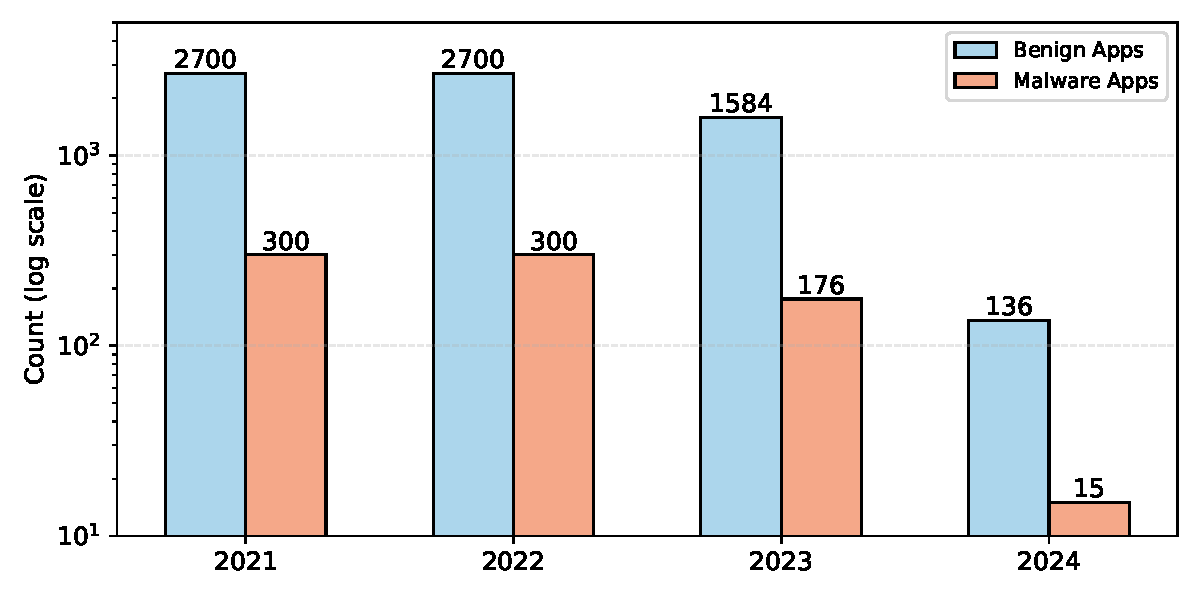
\includegraphics[width=0.68\linewidth]{fig/new_data.pdf}
    \vspace{-0.2cm}
    \caption{\DIFaddFL{Data statistics of apps collected from 2021 to 2024. The y axis uses a logarithmic scale.}}
    \label{fig:new_data}
    \vspace{-0.3cm}
\end{figure}

\subsubsection{\textbf{\DIFadd{Additional Dataset}}}
\label{additional_dataset}

\DIFadd{As a complementary dataset, we collect Android apps from different sources, }\textit{\DIFadd{i.e.,}} \DIFadd{AndroZoo~\mbox{%DIFAUXCMD
\cite{allix2016androzoo} }\hskip0pt%DIFAUXCMD
and VirusTotal~\mbox{%DIFAUXCMD
\cite{virustotal}}\hskip0pt%DIFAUXCMD
, spanning the years 2021 to 2024, following the same principles outlined above.
During this process, we observe that the number of malware samples in these years is relatively small, making it challenging to support a thorough evaluation~\mbox{%DIFAUXCMD
\cite{arp2022and}}\hskip0pt%DIFAUXCMD
.
To enrich the dataset, we therefore additionally gather malware samples from VirusShare~\mbox{%DIFAUXCMD
\cite{vs}}\hskip0pt%DIFAUXCMD
, a well-known repository that aggregates a large collection of malware from various sources.
We maintain a realistic goodware-to-malware ratio of 9:1 in this additional dataset.
Figure~\ref{fig:new_data} summarizes its statistics, which in total contains 7,911 apps, including 791 malicious and 7,120 benign samples.
We note that the number of malicious samples in this additional dataset is still relatively small compared to the primary dataset.
Nonetheless, it is sufficient to support our complementary experiments, which primarily aim to validate the findings from the main evaluation, particularly regarding the effectiveness (}\textit{\DIFadd{e.g.,}} \DIFadd{whether detection performance changes significantly) and efficiency (}\textit{\DIFadd{e.g.,}} \DIFadd{memory usage) of the selected approaches.
}

\DIFaddend \subsection{Effectiveness}
\label{effectiveness}
In this section, we examine how the \DIFaddbegin \DIFadd{detection }\DIFaddend effectiveness of the selected approaches varies \DIFdelbegin \DIFdel{across }\DIFdelend \DIFaddbegin \DIFadd{under }\DIFaddend different experimental settings\DIFdelbegin \DIFdel{to pinpoint the }\DIFdelend \DIFaddbegin \DIFadd{, with the goal of identifying the key }\DIFaddend factors that contribute to an effective malware detector.
Specifically, we focus on the following aspects: goodware-to-malware ratio, training set size, APK \DIFdelbegin \DIFdel{features}\DIFdelend \DIFaddbegin \DIFadd{feature choices}\DIFaddend , and model selection.
These factors are pivotal \DIFdelbegin \DIFdel{as }\DIFdelend \DIFaddbegin \DIFadd{because }\DIFaddend they influence the quality of the training data and the model's ability to extract relevant information, both of which are \DIFdelbegin \DIFdel{essential for }\DIFdelend \DIFaddbegin \DIFadd{critical to }\DIFaddend the performance of ML-based detectors.
\DIFaddbegin \DIFadd{All experiments in this section are conducted on the primary dataset (Section~\ref{sec:dataset}).
}\DIFaddend 

\begin{table}[t]
    \centering
    \renewcommand{\arraystretch}{0.9}
    \caption{The effectiveness \DIFaddbeginFL \DIFaddFL{(F1 and Accuracy) }\DIFaddendFL of the approaches across varied goodware-to-malware ratios in training and testing sets.}
    % \vspace{-0.1cm}
    \DIFdelbeginFL %DIFDELCMD < \begin{adjustbox}{width=0.74\linewidth, center}
%DIFDELCMD <  %%%
\DIFdelendFL \DIFaddbeginFL \begin{adjustbox}{width=0.84\linewidth, center}
 \DIFaddendFL \begin{tabular}{@{}c|cccc|cccc@{}}
     \toprule
     \DIFdelbeginFL %DIFDELCMD < \multirow{3}{*}{\textbf{\begin{tabular}[c]{@{}c@{}} Selected\\ Approach\end{tabular}}} %%%
\DIFdelendFL \DIFaddbeginFL \multirow{3}{*}{\textbf{\makecell[c]{Selected\\ Approach}}} \DIFaddendFL & \multicolumn{4}{c|}{\textbf{B:M=9:1 in Tr (\ding{182} - \ding{183})}}& \multicolumn{4}{c}{\textbf{B:M=1:1 in Tr (\ding{184} - \ding{185})}}\\ \cmidrule(l){2-9} 
     & \multicolumn{2}{c|}{\textbf{B:M=9:1 in Ts}}& \multicolumn{2}{c|}{\textbf{B:M=1:1 in Ts}}& \multicolumn{2}{c|}{\textbf{B:M=9:1 in Ts}}& \multicolumn{2}{c}{\textbf{B:M=1:1 in Ts}} \\ \cmidrule(l){2-9} 
     & \multicolumn{1}{c|}{\textbf{F1}} & \multicolumn{1}{c|}{\textbf{Acc.}} & \multicolumn{1}{c|}{\textbf{F1}} & \textbf{Acc.} & \multicolumn{1}{c|}{\textbf{F1}} & \multicolumn{1}{c|}{\textbf{Acc.}} & \multicolumn{1}{c|}{\textbf{F1}} & \textbf{Acc.} \\ \midrule
     Drebin & \multicolumn{1}{c|}{0.722}& \multicolumn{1}{c|}{\textbf{0.948}} & \multicolumn{1}{c|}{0.791}& 0.823 & \multicolumn{1}{c|}{0.650}& \multicolumn{1}{c|}{0.901} & \multicolumn{1}{c|}{0.918}& 0.917 \\ \midrule
     MamaDroid& \multicolumn{1}{c|}{0.661}& \multicolumn{1}{c|}{0.945} & \multicolumn{1}{c|}{0.693}& 0.763 & \multicolumn{1}{c|}{0.650}& \multicolumn{1}{c|}{0.902} & \multicolumn{1}{c|}{0.895}& 0.897 \\ \midrule
     Mclaughlin et al.& \multicolumn{1}{c|}{0.714}& \multicolumn{1}{c|}{0.946} & \multicolumn{1}{c|}{0.799}& 0.828 & \multicolumn{1}{c|}{0.682}& \multicolumn{1}{c|}{\textbf{0.924}} & \multicolumn{1}{c|}{0.916}& 0.916 \\ \midrule
     HinDroid & \multicolumn{1}{c|}{\textbf{0.731}}& \multicolumn{1}{c|}{0.943} & \multicolumn{1}{c|}{0.819}& 0.842 & \multicolumn{1}{c|}{\textbf{0.701}}& \multicolumn{1}{c|}{0.924} & \multicolumn{1}{c|}{\textbf{0.925}}& \textbf{0.925} \\ \midrule
     DeepRefiner & \multicolumn{1}{c|}{0.657}& \multicolumn{1}{c|}{0.932} & \multicolumn{1}{c|}{0.776}& 0.809 & \multicolumn{1}{c|}{0.667}& \multicolumn{1}{c|}{0.918} & \multicolumn{1}{c|}{0.881}& 0.881 \\ \midrule
     Kim et al.& \multicolumn{1}{c|}{\textbf{0.782}}& \multicolumn{1}{c|}{\textbf{0.952}} & \multicolumn{1}{c|}{\textbf{0.907}}& \textbf{0.912} & \multicolumn{1}{c|}{\textbf{0.753}}& \multicolumn{1}{c|}{0.\textbf{941}} & \multicolumn{1}{c|}{\textbf{0.938}}& \textbf{0.937} \\ \midrule
     MalScan& \multicolumn{1}{c|}{0.684}& \multicolumn{1}{c|}{0.939} & \multicolumn{1}{c|}{0.793}& 0.823 & \multicolumn{1}{c|}{0.587}& \multicolumn{1}{c|}{0.877} & \multicolumn{1}{c|}{0.880}& 0.880 \\ \midrule
     SDAC& \multicolumn{1}{c|}{0.522}& \multicolumn{1}{c|}{0.916} & \multicolumn{1}{c|}{0.627}& 0.720 & \multicolumn{1}{c|}{0.524}& \multicolumn{1}{c|}{0.850} & \multicolumn{1}{c|}{0.845}& 0.844 \\ \midrule
     HomDroid & \multicolumn{1}{c|}{\textbf{0.734}}& \multicolumn{1}{c|}{\textbf{0.949}} & \multicolumn{1}{c|}{0.816}& 0.841 & \multicolumn{1}{c|}{\textbf{0.701}}& \multicolumn{1}{c|}{\textbf{0.925}} & \multicolumn{1}{c|}{0.912}& 0.914 \\ \midrule
     Xmal& \multicolumn{1}{c|}{0.698}& \multicolumn{1}{c|}{0.942} & \multicolumn{1}{c|}{0.826}& \textbf{0.847} & \multicolumn{1}{c|}{0.674}& \multicolumn{1}{c|}{0.916} & \multicolumn{1}{c|}{\textbf{0.923}}& \textbf{0.924} \\ \midrule
     RAMDA& \multicolumn{1}{c|}{0.636}& \multicolumn{1}{c|}{0.905} & \multicolumn{1}{c|}{\textbf{0.841}}& \textbf{0.852} & \multicolumn{1}{c|}{0.510}& \multicolumn{1}{c|}{0.829} & \multicolumn{1}{c|}{0.871}& 0.865 \\ \midrule
     MSDroid& \multicolumn{1}{c|}{0.648}& \multicolumn{1}{c|}{0.919} & \multicolumn{1}{c|}{\textbf{0.834}}&0.828 & \multicolumn{1}{c|}{0.522}& \multicolumn{1}{c|}{0.853} & \multicolumn{1}{c|}{0.867}& 0.858 \\ \bottomrule
     \end{tabular}
    \end{adjustbox}
    \label{tab:res_ratio}
    \begin{tablenotes}[flushleft, labelsep=0]
 \footnotesize
 \item \textit{Tr:} training set, \textit{Ts:} testing set. \ding{182} - \ding{185} correspond to the four scenarios in Table~\ref{tab:effectiveness_dataset}. The top 3 results for each scenario are highlighted in bold.
 \end{tablenotes}
    \vspace{-0.5cm}
\end{table}

% We investigate how various factors --- goodware-to-malware ratio in training and testing sets, training set size, and APK feature --- affect the effectiveness of these approaches.

\DIFaddbegin \begin{table}[t]
    \centering
    \renewcommand{\arraystretch}{0.9}
    \caption{\DIFaddFL{The effectiveness (precision and recall) of the approaches across varied goodware-to-malware ratios in training and testing sets.}}
    \begin{adjustbox}{width=0.84\linewidth, center}
    \begin{tabular}{@{}c|cccc|cccc@{}}
     \toprule
    \multirow{3}{*}{\textbf{\makecell[c]{Selected\\ Approach}}}
     & \multicolumn{4}{c|}{\textbf{\DIFaddFL{B:M=9:1 in Tr (}\ding{182} \DIFaddFL{- }\ding{183}\DIFaddFL{)}}}
     & \multicolumn{4}{c}{\textbf{\DIFaddFL{B:M=1:1 in Tr (}\ding{184} \DIFaddFL{- }\ding{185}\DIFaddFL{)}}}\\ 
     \cmidrule[\cmidrulewidth](l){2-9} 
     & \multicolumn{2}{c|}{\textbf{\DIFaddFL{B:M=9:1 in Ts}}}
     & \multicolumn{2}{c|}{\textbf{\DIFaddFL{B:M=1:1 in Ts}}}
     & \multicolumn{2}{c|}{\textbf{\DIFaddFL{B:M=9:1 in Ts}}}
     & \multicolumn{2}{c}{\textbf{\DIFaddFL{B:M=1:1 in Ts}}} \\ 
     \cmidrule[\cmidrulewidth](l){2-9} 
     & \multicolumn{1}{c|}{\textbf{\DIFaddFL{Prec.}}} 
     & \multicolumn{1}{c|}{\textbf{\DIFaddFL{Rec.}}} 
     & \multicolumn{1}{c|}{\textbf{\DIFaddFL{Prec.}}} 
     & \textbf{\DIFaddFL{Rec.}} 
     & \multicolumn{1}{c|}{\textbf{\DIFaddFL{Prec.}}} 
     & \multicolumn{1}{c|}{\textbf{\DIFaddFL{Rec.}}} 
     & \multicolumn{1}{c|}{\textbf{\DIFaddFL{Prec.}}} 
     & \textbf{\DIFaddFL{Rec.}} \\ 
     \midrule

     \DIFaddFL{Drebin          }& \multicolumn{1}{c|}{\DIFaddFL{0.776}} & \multicolumn{1}{c|}{\DIFaddFL{0.675}} & \multicolumn{1}{c|}{\DIFaddFL{0.964}} & \DIFaddFL{0.671 }& \multicolumn{1}{c|}{\DIFaddFL{0.501}} & \multicolumn{1}{c|}{\DIFaddFL{0.925}} & \multicolumn{1}{c|}{\DIFaddFL{0.906}} & \DIFaddFL{0.930 }\\ \midrule
     \DIFaddFL{MamaDroid       }& \multicolumn{1}{c|}{\DIFaddFL{0.863}} & \multicolumn{1}{c|}{\DIFaddFL{0.535}} & \multicolumn{1}{c|}{\DIFaddFL{0.984}} & \DIFaddFL{0.535 }& \multicolumn{1}{c|}{\DIFaddFL{0.506}} & \multicolumn{1}{c|}{\DIFaddFL{0.910}} & \multicolumn{1}{c|}{\DIFaddFL{0.905}} & \DIFaddFL{0.886 }\\ \midrule
     \DIFaddFL{Mclaughlin et al.}& \multicolumn{1}{c|}{\DIFaddFL{0.758}} & \multicolumn{1}{c|}{\DIFaddFL{0.675}} & \multicolumn{1}{c|}{\DIFaddFL{0.958}} & \DIFaddFL{0.685 }& \multicolumn{1}{c|}{\DIFaddFL{0.584}} & \multicolumn{1}{c|}{\DIFaddFL{0.820}} & \multicolumn{1}{c|}{\DIFaddFL{0.908}} & \DIFaddFL{0.925 }\\ \midrule
     \DIFaddFL{HinDroid        }& \multicolumn{1}{c|}{\DIFaddFL{0.722}} & \multicolumn{1}{c|}{\DIFaddFL{0.740}} & \multicolumn{1}{c|}{\DIFaddFL{0.956}} & \DIFaddFL{0.717 }& \multicolumn{1}{c|}{\DIFaddFL{0.578}} & \multicolumn{1}{c|}{\DIFaddFL{0.890}} & \multicolumn{1}{c|}{\DIFaddFL{0.914}} & \DIFaddFL{0.937 }\\ \midrule
     \DIFaddFL{DeepRefiner     }& \multicolumn{1}{c|}{\DIFaddFL{0.663}} & \multicolumn{1}{c|}{\DIFaddFL{0.650}} & \multicolumn{1}{c|}{\DIFaddFL{0.944}} & \DIFaddFL{0.659 }& \multicolumn{1}{c|}{\DIFaddFL{0.562}} & \multicolumn{1}{c|}{\DIFaddFL{0.820}} & \multicolumn{1}{c|}{\DIFaddFL{0.883}} & \DIFaddFL{0.878 }\\ \midrule
     \DIFaddFL{Kim et al.      }& \multicolumn{1}{c|}{\DIFaddFL{0.717}} & \multicolumn{1}{c|}{\DIFaddFL{0.860}} & \multicolumn{1}{c|}{\DIFaddFL{0.960}} & \DIFaddFL{0.859 }& \multicolumn{1}{c|}{\DIFaddFL{0.644}} & \multicolumn{1}{c|}{\DIFaddFL{0.905}} & \multicolumn{1}{c|}{\DIFaddFL{0.922}} & \DIFaddFL{0.954 }\\ \midrule
     \DIFaddFL{MalScan         }& \multicolumn{1}{c|}{\DIFaddFL{0.704}} & \multicolumn{1}{c|}{\DIFaddFL{0.665}} & \multicolumn{1}{c|}{\DIFaddFL{0.954}} & \DIFaddFL{0.678 }& \multicolumn{1}{c|}{\DIFaddFL{0.442}} & \multicolumn{1}{c|}{\DIFaddFL{0.875}} & \multicolumn{1}{c|}{\DIFaddFL{0.878}} & \DIFaddFL{0.881 }\\ \midrule
     \DIFaddFL{SDAC            }& \multicolumn{1}{c|}{\DIFaddFL{0.632}} & \multicolumn{1}{c|}{\DIFaddFL{0.480}} & \multicolumn{1}{c|}{\DIFaddFL{0.908}} & \DIFaddFL{0.511 }& \multicolumn{1}{c|}{\DIFaddFL{0.379}} & \multicolumn{1}{c|}{\DIFaddFL{0.850}} & \multicolumn{1}{c|}{\DIFaddFL{0.835}} & \DIFaddFL{0.838 }\\ \midrule
     \DIFaddFL{HomDroid        }& \multicolumn{1}{c|}{\DIFaddFL{0.755}} & \multicolumn{1}{c|}{\DIFaddFL{0.714}} & \multicolumn{1}{c|}{\DIFaddFL{0.963}} & \DIFaddFL{0.708 }& \multicolumn{1}{c|}{\DIFaddFL{0.583}} & \multicolumn{1}{c|}{\DIFaddFL{0.879}} & \multicolumn{1}{c|}{\DIFaddFL{0.926}} & \DIFaddFL{0.898 }\\ \midrule
     \DIFaddFL{Xmal            }& \multicolumn{1}{c|}{\DIFaddFL{0.728}} & \multicolumn{1}{c|}{\DIFaddFL{0.670}} & \multicolumn{1}{c|}{\DIFaddFL{0.953}} & \DIFaddFL{0.729 }& \multicolumn{1}{c|}{\DIFaddFL{0.549}} & \multicolumn{1}{c|}{\DIFaddFL{0.875}} & \multicolumn{1}{c|}{\DIFaddFL{0.927}} & \DIFaddFL{0.920 }\\ \midrule
     \DIFaddFL{RAMDA           }& \multicolumn{1}{c|}{\DIFaddFL{0.516}} & \multicolumn{1}{c|}{\DIFaddFL{0.830}} & \multicolumn{1}{c|}{\DIFaddFL{0.910}} & \DIFaddFL{0.781 }& \multicolumn{1}{c|}{\DIFaddFL{0.357}} & \multicolumn{1}{c|}{\DIFaddFL{0.890}} & \multicolumn{1}{c|}{\DIFaddFL{0.829}} & \DIFaddFL{0.918 }\\ \midrule
     \DIFaddFL{MSDroid         }& \multicolumn{1}{c|}{\DIFaddFL{0.563}} & \multicolumn{1}{c|}{\DIFaddFL{0.760}} & \multicolumn{1}{c|}{\DIFaddFL{0.805}} & \DIFaddFL{0.866 }& \multicolumn{1}{c|}{\DIFaddFL{0.387}} & \multicolumn{1}{c|}{\DIFaddFL{0.800}} & \multicolumn{1}{c|}{\DIFaddFL{0.820}} & \DIFaddFL{0.919 }\\

     \bottomrule
     \end{tabular}
    \end{adjustbox}
    \label{tab:res_ratio_prec_rec}
    \begin{tablenotes}[flushleft, labelsep=0]
    \footnotesize
    \item \textit{\DIFaddFL{Tr:}} \DIFaddFL{training set, }\textit{\DIFaddFL{Ts:}} \DIFaddFL{testing set. }\ding{182} \DIFaddFL{- }\ding{185} \DIFaddFL{correspond to the four scenarios in Table~\ref{tab:effectiveness_dataset}. The top 3 results for each scenario are highlighted in bold.
    }\end{tablenotes}
    \vspace{-0.5cm}
\end{table}
\DIFaddend \bulletpoint{Goodware-to-malware ratio}
The effectiveness of ML-based Android malware detectors is heavily influenced by malware distributions in the training and testing sets.
Here, we consider two ratios, \textit{i.e.}, 10\%, and 50\%, in both training and testing sets.
These choices are inspired by the estimated 10\% in the wild~\DIFdelbegin \DIFdel{\mbox{%DIFAUXCMD
\cite{pendlebury2019tesseract} }\hskip0pt%DIFAUXCMD
}\DIFdelend \DIFaddbegin \DIFadd{\mbox{%DIFAUXCMD
\cite{pendlebury2019tesseract,chen2023continuous} }\hskip0pt%DIFAUXCMD
}\DIFaddend and the 50\% widely used in previous studies~\cite{wu2019malscan,li2021robust,mariconti2016mamadroid}.
The \ding{182} - \ding{185} in Table~\ref{tab:effectiveness_dataset} present these four scenarios\DIFaddbegin \DIFadd{, where }\ding{182} \DIFadd{and }\ding{183} \DIFadd{have a 10\% malware ratio in training sets, while }\ding{184} \DIFadd{and }\ding{185} \DIFadd{have a 50\% malware ratio}\DIFaddend .

Table~\ref{tab:res_ratio} summarizes the results in terms of F1-score and Accuracy.
The results are arranged from left to right, \DIFdelbegin \DIFdel{mapping }\DIFdelend \DIFaddbegin \DIFadd{corresponding to }\DIFaddend scenarios \ding{182} \DIFdelbegin \DIFdel{to }\DIFdelend \DIFaddbegin \DIFadd{through }\DIFaddend \ding{185}.
We observe that all \DIFdelbegin \DIFdel{the approaches produce promising results }\DIFdelend \DIFaddbegin \DIFadd{approaches achieve promising performance in all metrics }\DIFaddend under scenario \ding{185}, \DIFaddbegin \DIFadd{which is }\DIFaddend characterized by a \texttt{1:1} goodware-to-malware ratio in both \DIFaddbegin \DIFadd{the }\DIFaddend training and testing sets.
\DIFaddbegin \DIFadd{These findings are consistent with the results reported in the original papers, confirming the validity of our re-implementations. 
}\DIFaddend This demonstrates that these approaches can effectively detect Android malware under ideal conditions, where goodware and malware are balanced.
However, when the malware \DIFdelbegin \DIFdel{ratio is adjusted }\DIFdelend \DIFaddbegin \DIFadd{proportion is reduced }\DIFaddend to 10\% (\ding{182}), there is a \DIFdelbegin \DIFdel{marked decline in the }\DIFdelend \DIFaddbegin \DIFadd{pronounced decline in }\DIFaddend F1-score across all methods.
%DIF <  It is evident that most of these approaches suffer from performance degradation when faced with a realistic malware ratio.
%DIF <  This is primarily due to the limited number of malware samples available for training, which hampers the model's ability to learn effective patterns.
%DIF <  Additionally, by increasing the malware ratio in testing sets from 10\% to 50\% (\ding{183} and \ding{185}), we notice the F1-scores increase for all methods.
%DIF <  This is expected, as the increased number of malware samples in the testing set makes models more likely to encounter familiar patterns, leading to improved performance.
%DIF <  For a coarse and aggregate analysis, upon analyzing the top three results, we find that DL-based approaches appear to outperform TML-based methods when the malware ratio is 50\% (\ding{183} and \ding{185}) --- almost all the top three results are achieved by DL-based methods.
%DIF <  While in more realistic scenarios (\ding{182} and \ding{184}), DL-based approaches do not exhibit a marked advantage over TML-based methods.
It is evident that many existing approaches experience performance degradation when evaluated under realistic malware ratios.
This is primarily attributed to the scarcity of malware samples in the training data, which constrains the model's ability to learn discriminative malware semantics.
Moreover, when the malware ratio in the test set is increased from 10\% to 50\% (\ding{183} and \ding{185}), we observe a consistent improvement in F1-scores across all methods.
This trend is expected, as a higher prevalence of malware samples in the test set increases the likelihood that models will encounter patterns similar to those seen during training, enhancing their predictive performance.
\DIFdelbegin \DIFdel{In }\DIFdelend \DIFaddbegin \DIFadd{To more clearly reveal the performance differences between deep learning (DL)-based and traditional machine learning (TML)-based approaches, we conduct }\DIFaddend a coarse-grained, \DIFdelbegin \DIFdel{average analysis , where }\DIFdelend \DIFaddbegin \DIFadd{averaged analysis of the results, as averaging can partially mitigate }\DIFaddend the influence of \DIFaddbegin \DIFadd{the }\DIFaddend differing feature combinations \DIFdelbegin \DIFdel{is partially mitigated due to the diverse features used by both TML-based and DL-based approaches, we find }\DIFdelend \DIFaddbegin \DIFadd{employed by both types of approaches.
We observe }\DIFaddend an interesting phenomenon: DL-based approaches appear to outperform TML-based methods when the testing malware ratio is 50\% (\ding{183} and \ding{185}) --- almost all the top three results are achieved by DL-based methods.
While in more realistic scenarios (\ding{182} and \ding{184}), DL-based approaches do not exhibit a \DIFdelbegin \DIFdel{marked }\DIFdelend \DIFaddbegin \DIFadd{pronounced }\DIFaddend advantage over TML-based methods.
One possible explanation is that DL-based methods are better equipped to capture the complex semantics underlying app behaviors, \DIFaddbegin \DIFadd{but require more malware samples to effectively distill such semantics, }\DIFaddend which tend to be more prominent in datasets with a higher malware ratio.
% This is because malware samples are typically more diverse and intricate, presenting greater challenges for detection.



\DIFaddbegin \DIFadd{Table~\ref{tab:res_ratio_prec_rec} provides Precision and Recall values for these scenarios.
When the training set ratio is fixed, we observe that the malware detection performance (in terms of Recall) does not change significantly as the testing set ratio varies, as shown by pairs }\ding{182}\DIFadd{-}\ding{183} \DIFadd{and }\ding{184}\DIFadd{-}\ding{185} \DIFadd{in Table~\ref{tab:res_ratio_prec_rec}. 
In contrast, when the testing set ratio is fixed, we find that the Recall improves as the training set ratio increases from 10\% to 50\%, as illustrated by pairs }\ding{182}\DIFadd{-}\ding{184} \DIFadd{and }\ding{183}\DIFadd{-}\ding{185} \DIFadd{in Table~\ref{tab:res_ratio_prec_rec}.
This indicates that having a higher proportion of malware samples in the training set enhances the model's ability to learn effective malicious patterns, thereby improving detection accuracy.
}

\begin{figure}[t]
    \centering
    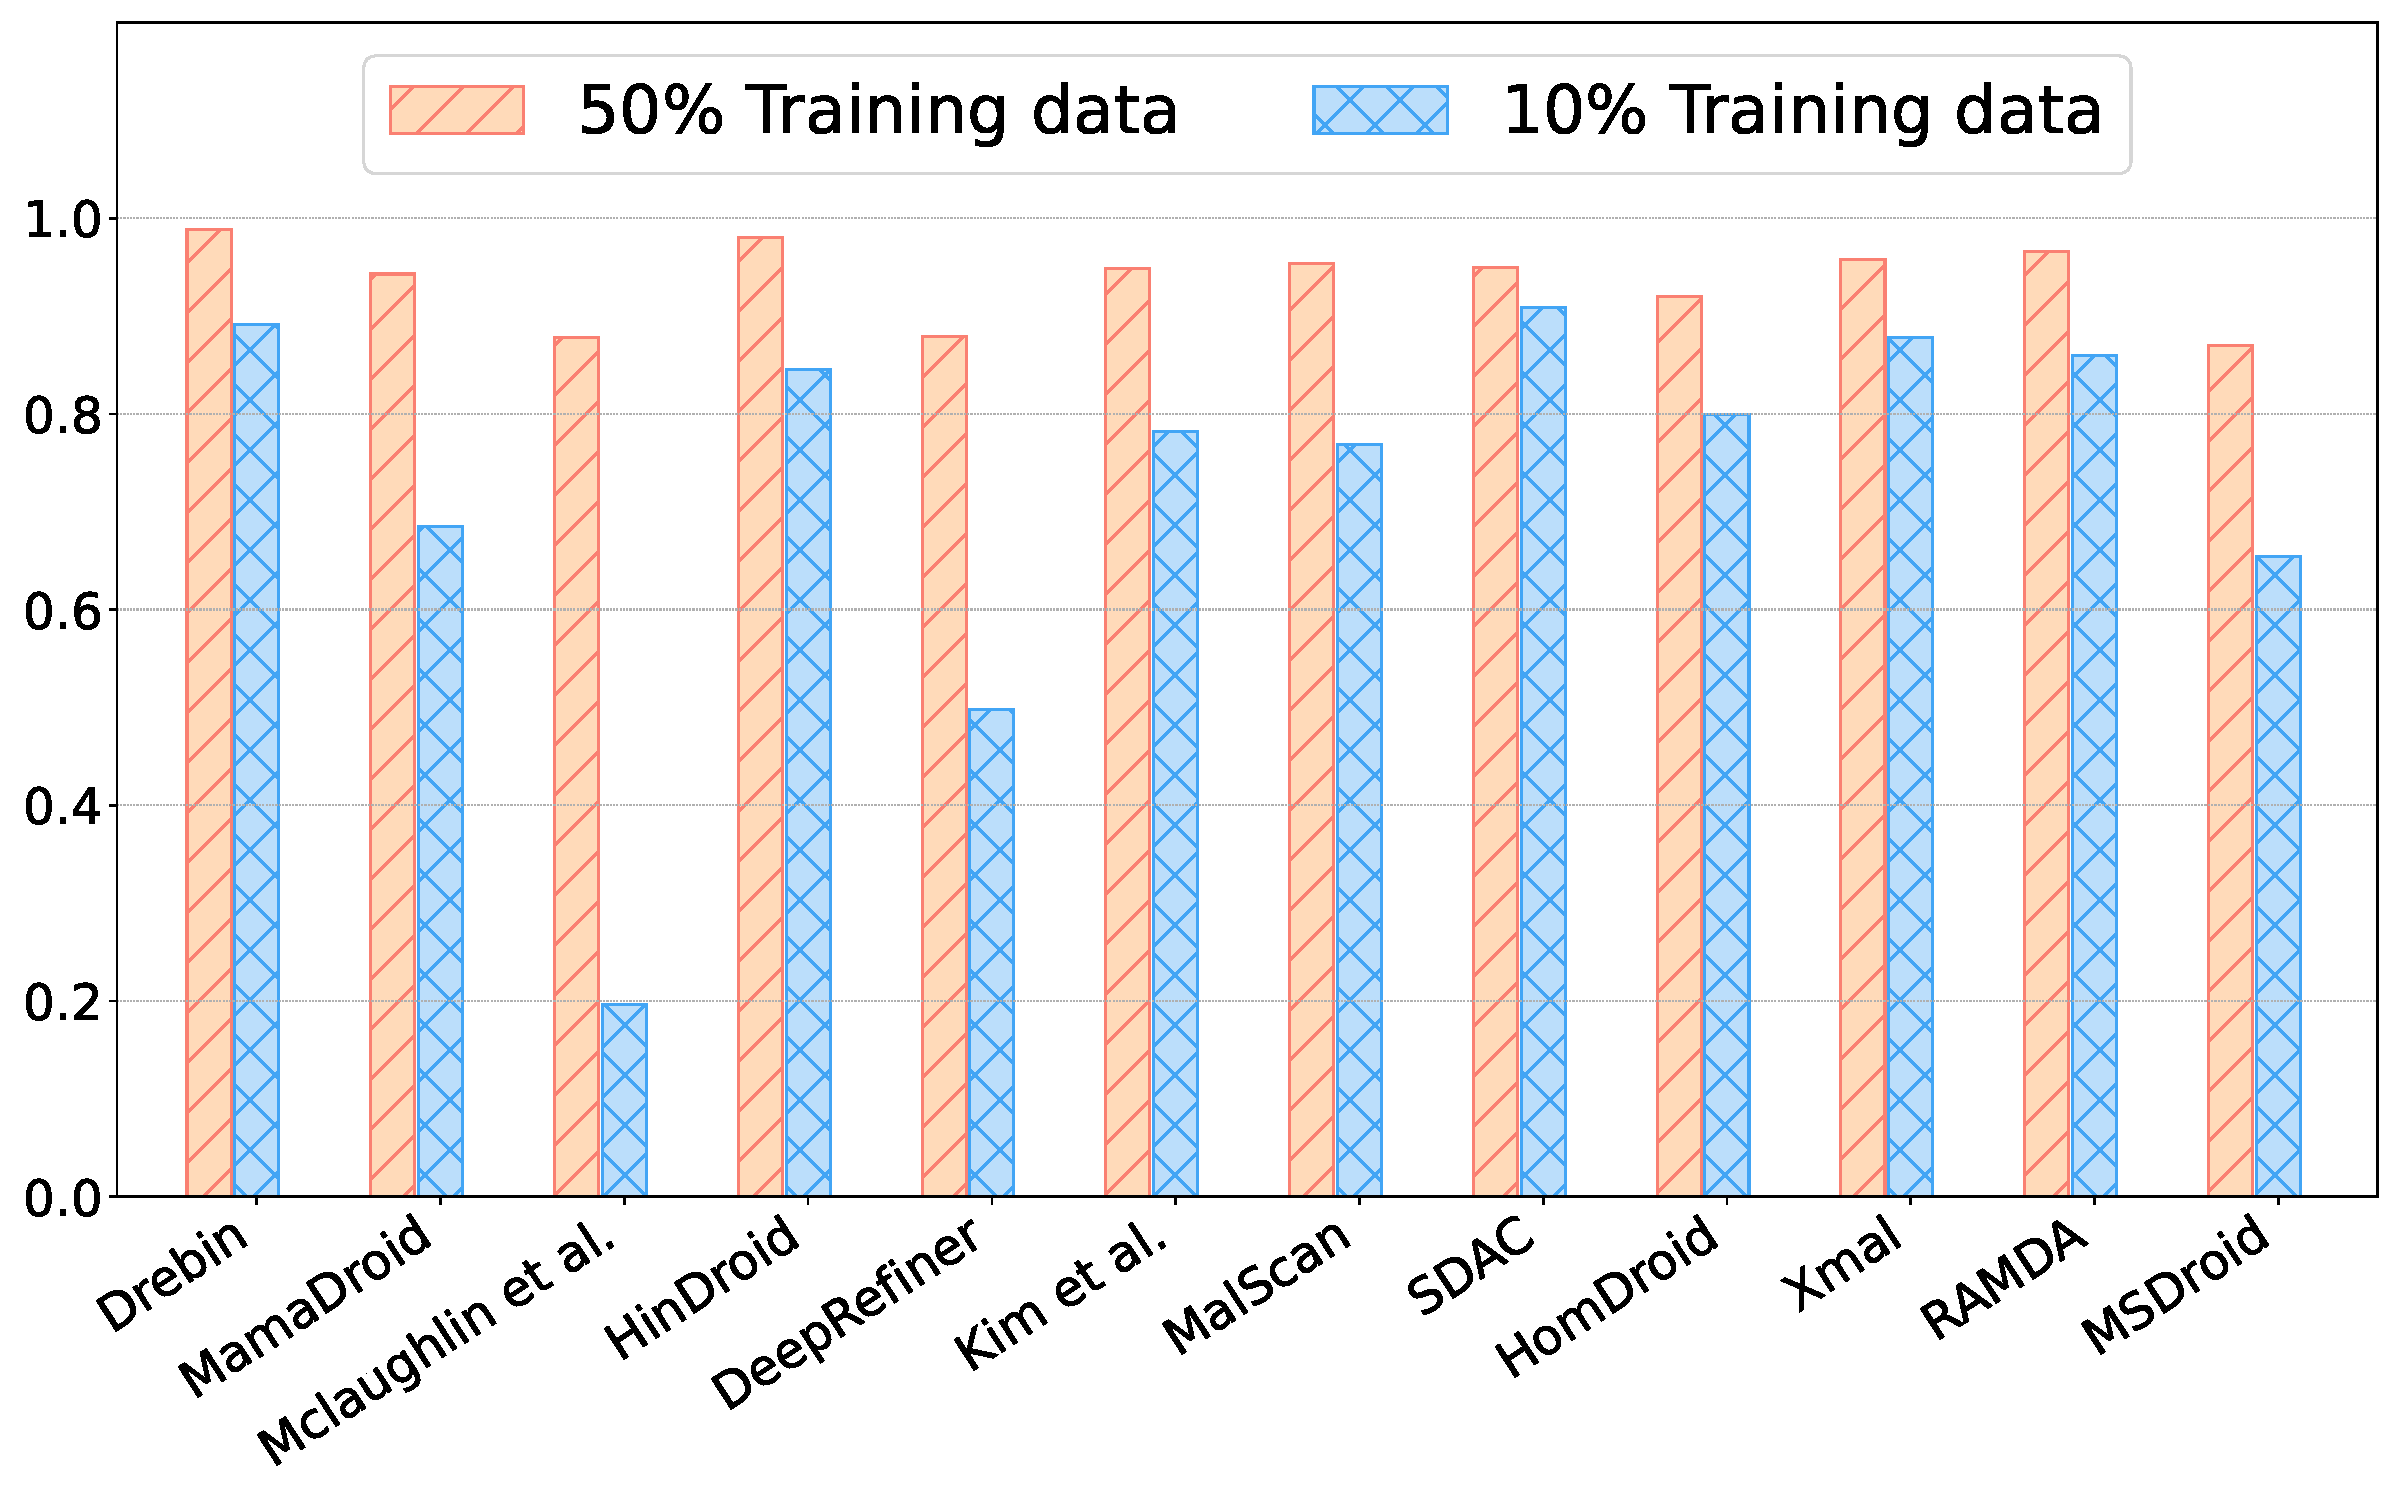
\includegraphics[width=0.8\linewidth]{fig/training_size.pdf}
    \vspace{-0.2cm}
    \caption{\DIFaddFL{Effectiveness of the selected approaches using different sizes of training data.}}
    \label{fig:training_size}
    \vspace{-0.5cm}
\end{figure}

\DIFaddend \bulletpoint{Training set size}
\DIFdelbegin \DIFdel{The training set 's size }\DIFdelend \DIFaddbegin \DIFadd{The size of the training set }\DIFaddend is a critical determinant of the effectiveness of ML classifiers~\cite{sun2017revisiting}, \DIFdelbegin \DIFdel{since }\DIFdelend \DIFaddbegin \DIFadd{as larger, }\DIFaddend high-quality \DIFdelbegin \DIFdel{training data typically provides }\DIFdelend \DIFaddbegin \DIFadd{datasets typically provide }\DIFaddend richer semantic information about malware, which is essential for learning effective classifiers.
However, \DIFdelbegin \DIFdel{securing a }\DIFdelend \DIFaddbegin \DIFadd{obtaining such }\DIFaddend large, high-quality training \DIFdelbegin \DIFdel{set }\DIFdelend \DIFaddbegin \DIFadd{sets }\DIFaddend is often infeasible due to the \DIFdelbegin \DIFdel{significant costs of }\DIFdelend \DIFaddbegin \DIFadd{substantial costs associated with }\DIFaddend data collection and labeling.
% Thus, we experiment with varying training set sizes to simulate different levels of semantic richness. 
% This assumption is justified by the fact that, as more data is included, a broader spectrum of malware semantics is likely to be captured, since our dataset is collected from multiple sources and spans a wide range of years, reflecting the real-world distribution of Android apps.
\DIFdelbegin \DIFdel{Thus}\DIFdelend \DIFaddbegin \DIFadd{In this experiment}\DIFaddend , we experiment with different training set sizes to simulate varying levels of semantic richness (\textit{i.e.,} larger datasets are assumed to encompass more diverse malware semantics) and analyze their impact on classifier performance.
Specifically, we consider two training set sizes, 50\% and 10\% of the original training set size, while maintaining the malware ratio at 10\%.
% To study the impact of training set size, we down-sample the training set in Table~\ref{tab:effectiveness_dataset}(\ding{182}) to 50\% and 10\% of its initial size, while ensuring that the malware ratio remains 10\%.

Figure~\ref{fig:training_size} shows how these detectors' performance changes when the training set size or semantic richness is reduced.
We normalize the F1-scores of these methods based on their performance obtained with the entire original dataset.
The detailed results are provided in the Appendix~\ref{sec:additional_results}.
The figure clearly shows that reducing the training set size leads to performance degradation across all approaches, underscoring more data enhances capturing malicious patterns.
Interestingly, Mclaughlin et al. and DeepRefiner display a greater sensitivity to training set size compared to others.
One explanation is that, unlike other methods that heuristically select features from apps, these two approaches take the original apps' bytecode as input and automatically extract semantics, requiring more data to learn patterns from raw data as opposed to hand-crafted features.
This finding highlights that the effectiveness of malware detectors is closely tied to the quality of the training data and the semantic richness it provides.
\DIFdelbegin \DIFdel{Also, it suggests that heuristic }\DIFdelend \DIFaddbegin \DIFadd{Furthermore, these findings suggest that carefully }\DIFaddend selected features that \DIFdelbegin \DIFdel{are semantically rich can be more effective than raw data in scenarios where data }\DIFdelend \DIFaddbegin \DIFadd{better capture malware semantics are crucial for effective detection, especially when training data }\DIFaddend is limited.
\DIFaddbegin \DIFadd{In contrast, models that learn directly from raw data often struggle to perform well under such data-scarce conditions.
}\DIFaddend 


%DIF >  Also, it suggests that heuristic selected features that are semantically rich can be more effective than raw data in scenarios where data is limited.
\DIFaddbegin 


\DIFaddend % {\bf This finding highlights the importance of feature selection in ML-based Android malware detection, especially in scenarios where data is limited.} The features selected needs to be related to the semantics of malware, where further work is needed to quantify the relevance. We also carry out an analysis on how the level of relevance in semantics affects effectiveness. 

% \tdsc{It's better to have a conclusion for Sec. 5.3.}

\DIFdelbegin %DIFDELCMD < \begin{figure}[t]
%DIFDELCMD <     \centering
%DIFDELCMD <     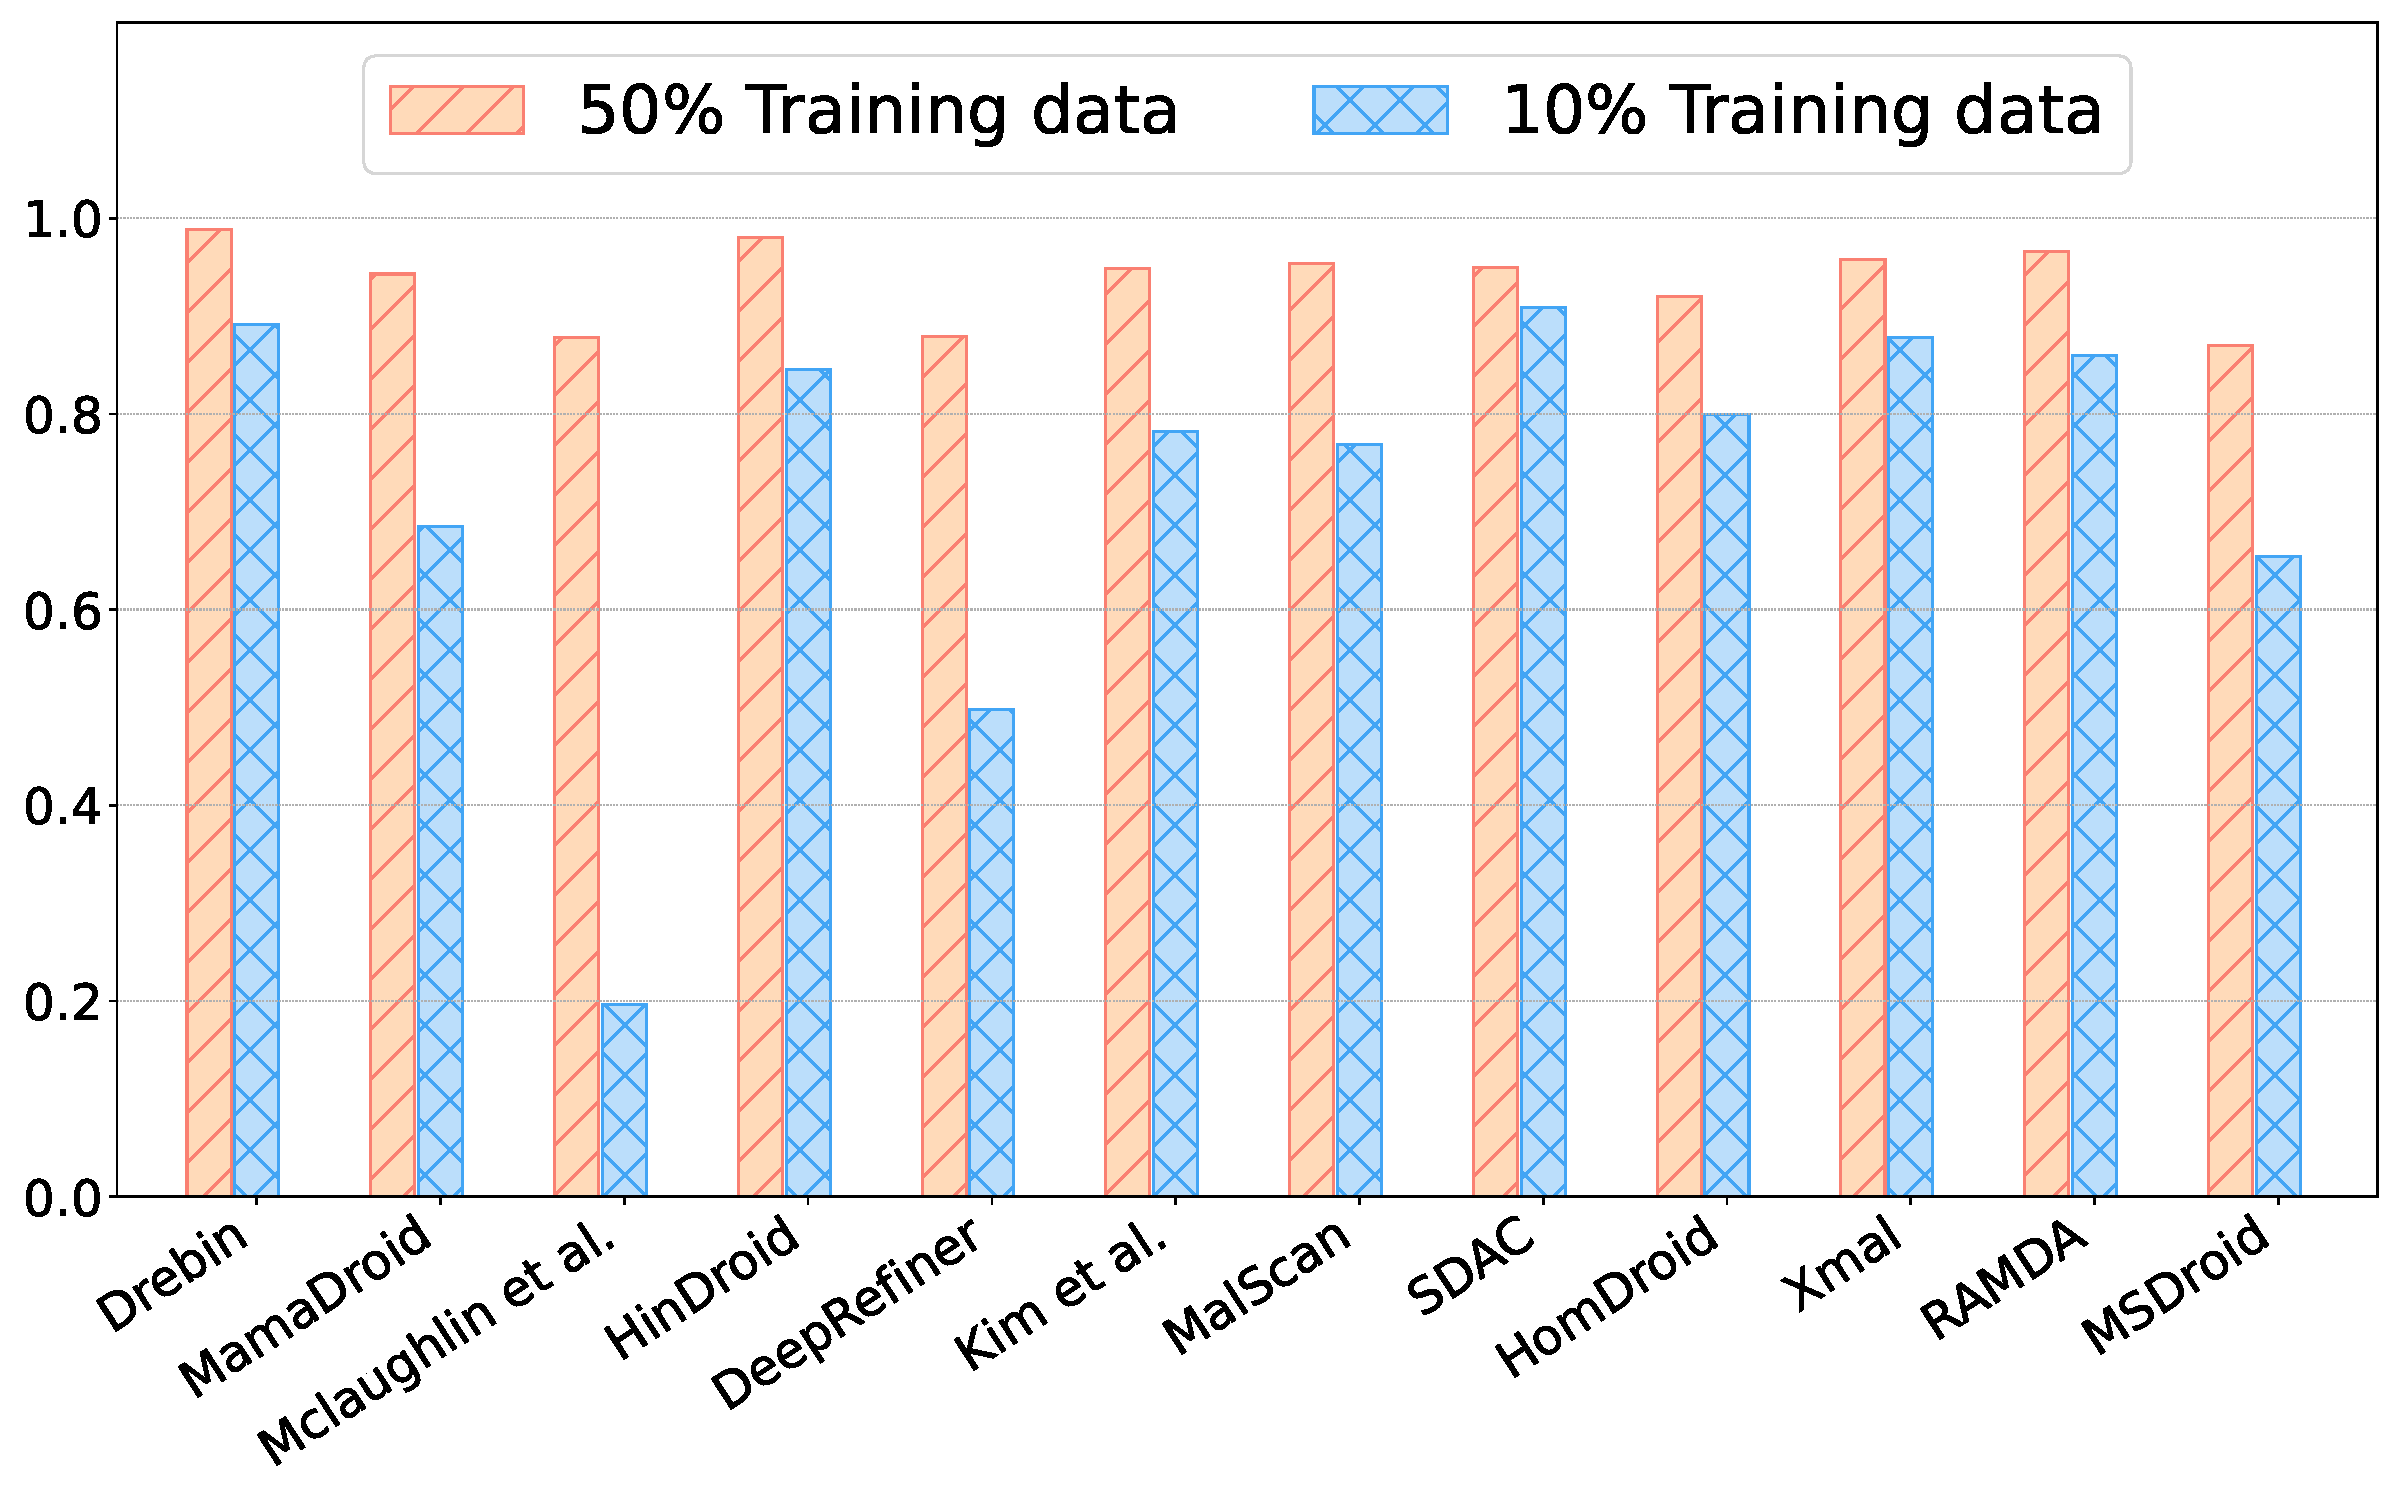
\includegraphics[width=0.64\linewidth]{fig/training_size.pdf}
%DIFDELCMD <     \vspace{-0.2cm}
%DIFDELCMD <     %%%
%DIFDELCMD < \caption{%
{%DIFAUXCMD
\DIFdelFL{Effectiveness of the selected approaches using different sizes of training data.}}
    %DIFAUXCMD
%DIFDELCMD < \label{fig:training_size}
%DIFDELCMD <     \vspace{-0.5cm}
%DIFDELCMD < \end{figure}
%DIFDELCMD < 

%DIFDELCMD < %%%
\DIFdelend % \subsection{Effectiveness vs. Semantics Levels\tdsc{(Domain Semantics?)}}

\bulletpoint{APK feature}
Android malware detectors often leverage diverse features to enhance detection performance~\cite{arp2014drebin,kim2018multimodal,li2021robust}.
The reason is that each feature contributes to characterizing APKs, encoding their unique semantics.
One question arises: does the incorporation of more features necessarily enhance a detector's performance?
To investigate this, we remove individual features from the original feature set to assess the resulting performance.
For this experiment, it is essential that the \DIFaddbegin \DIFadd{required }\DIFaddend features of the chosen approaches are decomposable, allowing the sequential removal of individual features.
Accordingly, we spotlight Drebin, Kim et al., Xmal, and RAMDA, owing to their decomposable feature sets.
We exclude methods whose features are highly intertwined.
For instance, MamaDroid and MalScan rely on specific API calls to extract features from program graphs, making it challenging to remove individual features --- if API calls are removed, the graph features will also be removed.

\DIFdelbegin \DIFdel{Table~\ref{tab:combination_feats} presents the outcomes of this experiment.
From the table, we observe that Drebin, Xmal, and RAMDA have performance degradation when one feature is removed.
Interestingly, Kim et al. deviate from this trend.
In fact, even after omitting several features, its performance exceeds the original results.
These two observations underscore:
(i) each feature contains unique semantics describing the APKs and contributes to the overall effectiveness of a malware detector, and (ii) the semantics of different feature sets are not always complementary, and merely expanding the feature set does not guarantee enhanced performance.
This phenomenon underscores the importance of evaluating and justifying the inclusion of each feature in a malware detector based on the semantics.
}%DIFDELCMD < 

%DIFDELCMD < %%%
%DIF <  These two observations underscore that each feature contributes to the overall effectiveness of a malware detector.
%DIF <  While in some cases, merely expanding the feature set does not guarantee enhanced performance.
%DIFDELCMD < 

%DIFDELCMD < %%%
%DIF <  {\bf This phenomenon underscores the importance of evaluating and justifying the inclusion of each feature in a malware detector based on the semantics.}
%DIFDELCMD < 

%DIFDELCMD < %%%
\DIFdelend \begin{table}[t]
    \centering
    \renewcommand{\arraystretch}{0.8}
    \caption{The impact of APK features on the effectiveness of Drebin, Kim et al., Xmal, and RAMDA.}
    % \vspace{-0.1cm}
    \begin{adjustbox}{width=0.86\linewidth, center}
 \begin{tabular}{@{}l|cc|cc|cc|cc@{}}
 \toprule
 \multirow{2}{*}{\textbf{\raisebox{-0.2cm}{\begin{tabular}[c]{@{}l@{}}Feature\\ Combination\end{tabular}}}} & \multicolumn{2}{c|}{\textbf{Drebin}}      & \multicolumn{2}{c|}{\textbf{Kim et al.}}  & \multicolumn{2}{c|}{\textbf{Xmal}} & \multicolumn{2}{c}{\textbf{RAMDA}} \\ \cmidrule(l){2-9} 
 & \multicolumn{1}{c|}{\textbf{F1}} & \textbf{Acc.} & \multicolumn{1}{c|}{\textbf{F1}} & \textbf{Acc.} & \multicolumn{1}{c|}{\textbf{F1}} & \textbf{Acc.} & \multicolumn{1}{c|}{\textbf{F1}} & \textbf{Acc.} \\ \midrule
 Original   & \multicolumn{1}{c|}{\textbf{0.722}}& \textbf{0.948}  & \multicolumn{1}{c|}{0.726}& 0.944  & \multicolumn{1}{c|}{\textbf{0.698}}& \textbf{0.942}  & \multicolumn{1}{c|}{\textbf{0.636}}& \textbf{0.905}  \\ \midrule
 w/o hardware& \multicolumn{1}{c|}{0.717}& 0.947  & \multicolumn{1}{c|}{0.728}& 0.945  & \multicolumn{1}{c|}{N/A}  & N/A    & \multicolumn{1}{c|}{N/A}  & N/A    \\ \midrule
 w/o app-intent & \multicolumn{1}{c|}{0.622}& 0.936  & \multicolumn{1}{c|}{\textbf{0.776}}& \textbf{0.952}  & \multicolumn{1}{c|}{N/A}  & N/A    & \multicolumn{1}{c|}{0.428}& 0.845  \\ \midrule
 w/o permission & \multicolumn{1}{c|}{0.698}& 0.945  & \multicolumn{1}{c|}{0.692}& 0.939  & \multicolumn{1}{c|}{0.566}& 0.926  & \multicolumn{1}{c|}{0.526}& 0.882  \\ \midrule
 w/o api call& \multicolumn{1}{c|}{0.691}& 0.944  & \multicolumn{1}{c|}{0.699}& 0.942  & \multicolumn{1}{c|}{0.639}& 0.930  & \multicolumn{1}{c|}{0.482}& 0.880  \\ \midrule
 w/o opcode & \multicolumn{1}{c|}{N/A}  & N/A    & \multicolumn{1}{c|}{0.724}& 0.942  & \multicolumn{1}{c|}{N/A}  & N/A    & \multicolumn{1}{c|}{N/A}  & N/A    \\ \midrule
 w/o code string& \multicolumn{1}{c|}{0.702}& 0.944  & \multicolumn{1}{c|}{0.725}& 0.945  & \multicolumn{1}{c|}{N/A}  & N/A    & \multicolumn{1}{c|}{N/A}  & N/A    \\ \bottomrule
 \end{tabular}
    \end{adjustbox}
    \label{tab:combination_feats}
    % \centering
    \begin{tablenotes}[flushleft, labelsep=0]
 \footnotesize
 \item \noindent w/o means without. N/A denotes features are not used in the original work.
 \end{tablenotes}
    \DIFdelbeginFL %DIFDELCMD < \vspace{-0.5cm}
%DIFDELCMD < %%%
\DIFdelendFL \DIFaddbeginFL \vspace{-0.3cm}
\DIFaddendFL \end{table}

\DIFaddbegin \DIFadd{Table~\ref{tab:combination_feats} presents the outcomes of this experiment.
From the table, we observe that Drebin, Xmal, and RAMDA have performance degradation when one feature is removed.
This is intuitive, that each feature contains unique semantics describing the APKs and contributes to the overall effectiveness of a malware detector.
Interestingly, Kim et al. deviate from this trend.
In fact, even after omitting several features, its performance exceeds the original results.
For example, removing the app-intent features, the F1-score improves from 0.726 to 0.776, and Accuracy increases from 0.944 to 0.952.
These two observations underscore:
(i) each feature contains unique semantics describing the APKs and contributes to the overall effectiveness of a malware detector, and 
(ii) in some cases (}\textit{\DIFadd{e.g.,}} \DIFadd{specifc models or feature combination style), simply expanding the feature set does not guarantee enhanced performance.
This phenomenon underscores the importance of evaluating and justifying the inclusion of each feature in a malware detector based on the semantics.
}

\DIFadd{It is important to note that we further examine the impact of feature combinations on the approach proposed by Kim et al. by varying the number of training epochs, in order to verify whether the observed phenomenon persists across different model configurations. Specifically, we set the training epochs to 50, 100, 150, and 200, and repeat the app-intent removal experiment under each setting to assess result consistency.
As shown in Table~\ref{tab:ablation_app_intent}, removing the app-intent feature consistently improves performance across all training epochs, in terms of both F1-score and accuracy. This demonstrates that the observed behavior is robust and not an artifact of a particular training configuration or convergence state.
These findings highlight an important insight: under certain conditions—such as specific classifiers or feature-combination strategies—the inclusion of additional features does not necessarily enhance detection performance and may even be detrimental. Consequently, researchers and practitioners should critically assess the contribution of individual features to overall model performance, rather than assuming that incorporating more features will invariably yield better results.
}

\begin{table}[h]
\centering
\caption{\DIFaddFL{Ablation study on the impact of app-intent information across different training epochs.}}
\label{tab:ablation_app_intent}
\begin{adjustbox}{width=0.63\linewidth, center}
\begin{tabular}{llcccc}
\toprule
\textbf{\DIFaddFL{Method}} & \textbf{\DIFaddFL{Metric}} & \textbf{\DIFaddFL{50}} & \textbf{\DIFaddFL{100}} & \textbf{\DIFaddFL{150}} & \textbf{\DIFaddFL{200}} \\
\midrule
\multirow{2}{*}{w/o app-intent}
& \DIFaddFL{F-Score  }& \DIFaddFL{0.740 }& \DIFaddFL{0.776 }& \DIFaddFL{0.753 }& \DIFaddFL{0.753 }\\
& \DIFaddFL{Accuracy }& \DIFaddFL{0.947 }& \DIFaddFL{0.952 }& \DIFaddFL{0.950 }& \DIFaddFL{0.950 }\\
\midrule
\multirow{2}{*}{original}
& \DIFaddFL{F-Score  }& \DIFaddFL{0.725 }& \DIFaddFL{0.725 }& \DIFaddFL{0.740 }& \DIFaddFL{0.738 }\\
& \DIFaddFL{Accuracy }& \DIFaddFL{0.944 }& \DIFaddFL{0.944 }& \DIFaddFL{0.952 }& \DIFaddFL{0.942 }\\
\bottomrule
\end{tabular}
\end{adjustbox}
\vspace{-0.4cm}
\end{table}

\DIFaddend \bulletpoint{Model type}
Given specific features that describe app behaviors, different models can be used to extract semantics and detect malware.
The features reflect the richness of the available semantics, while the models determine how effectively these semantics are leveraged.
In this section, we select MamaDroid, HinDroid, and MalScan, which share the same feature set and feature representation, as shown in Table~\ref{tbl:systematization}, to evaluate the impact of different models on the effectiveness of malware detectors.
From the results in Table~\ref{tab:res_ratio} under scenario \ding{182}, we observe that HinDroid outperforms MamaDroid and MalScan.
This suggests that given a fixed feature set, different models demonstrate varying capabilities in extracting semantics and detecting Android malware.

\DIFaddbegin \begin{table}[ht]
  \centering
  \caption{\DIFaddFL{Performance of common ML models across API and permission feature subsets.}}
  \label{tab:model_comparison}
  \begin{adjustbox}{width=0.87\linewidth}
    \begin{tabular}{lcccccc}
      \toprule
      \multirow{2}{*}{\textbf{Model}} &
        \multicolumn{2}{c}{\textbf{\DIFaddFL{API+Permission}}} &
        \multicolumn{2}{c}{\textbf{\DIFaddFL{API}}} &
        \multicolumn{2}{c}{\textbf{\DIFaddFL{Permission}}} \\
      \cmidrule[\cmidrulewidth](lr){2-3}\cmidrule[\cmidrulewidth](lr){4-5}\cmidrule[\cmidrulewidth](lr){6-7}
      & \textbf{\DIFaddFL{Accuracy}} & \textbf{\DIFaddFL{F1-score}} & \textbf{\DIFaddFL{Accuracy}} & \textbf{\DIFaddFL{F1-score}} & \textbf{\DIFaddFL{Accuracy}} & \textbf{\DIFaddFL{F1-score}} \\
      \midrule
      \DIFaddFL{RandomForest }& \DIFaddFL{0.984 }& \DIFaddFL{0.929 }& \DIFaddFL{0.975 }& \DIFaddFL{0.897 }& \DIFaddFL{0.973 }& \DIFaddFL{0.868 }\\
      \DIFaddFL{SVM          }& \DIFaddFL{0.978 }& \DIFaddFL{0.897 }& \DIFaddFL{0.975 }& \DIFaddFL{0.897 }& \DIFaddFL{0.962 }& \DIFaddFL{0.794 }\\
      \DIFaddFL{DecisionTree }& \DIFaddFL{0.984 }& \DIFaddFL{0.927 }& \DIFaddFL{0.965 }& \DIFaddFL{0.857 }& \DIFaddFL{0.959 }& \DIFaddFL{0.819 }\\
      \DIFaddFL{KNN          }& \DIFaddFL{0.973 }& \DIFaddFL{0.865 }& \DIFaddFL{0.975 }& \DIFaddFL{0.897 }& \DIFaddFL{0.954 }& \DIFaddFL{0.761 }\\
      \DIFaddFL{MLP          }& \DIFaddFL{0.981 }& \DIFaddFL{0.916 }& \DIFaddFL{0.973 }& \DIFaddFL{0.886 }& \DIFaddFL{0.973 }& \DIFaddFL{0.872 }\\
      \bottomrule
    \end{tabular}
  \end{adjustbox}
  \vspace{-0.3cm}
\end{table}

\DIFadd{Beyond analyzing existing approaches, we conduct a small-scale empirical study to examine how different learning models perform given a fixed feature set. Specifically, we select two widely used feature types—API calls and permissions—to represent app behavior, and evaluate five representative models commonly adopted in Android malware detection: Random Forest, SVM, Decision Tree, KNN, and MLP.
For this experiment, we use the dataset shown in Figure~\ref{fig:new_data} and randomly sample 4,000 apps (3,600 benign and 400 malicious). The dataset is split into training, validation, and testing sets using an }\texttt{\DIFadd{8:1:1}} \DIFadd{ratio.
}

\DIFadd{Intuitively, there is no universally optimal model for Android malware detection, as model performance is closely tied to the choice of feature representation. As shown in Table~\ref{tab:model_comparison}, when API calls are used as features, all evaluated classifiers achieve comparable performance. In contrast, when using permissions alone, MLP significantly outperforms the other models. When combining API calls and permission features, Random Forest achieves the best overall performance, with an accuracy of 98.4\% and an F1-score of 92.9\%.
Overall, our results suggest that ensemble-based models (}\textit{\DIFadd{e.g.}}\DIFadd{, Random Forest) and deep learning models (}\textit{\DIFadd{e.g.}}\DIFadd{, MLP) generally outperform other traditional classifiers (}\textit{\DIFadd{e.g.}}\DIFadd{, SVM, Decision Tree, and KNN) in Android malware detection tasks. Consequently, when designing new detectors, these models represent strong and practical baseline choices.
}



\DIFaddend \begin{conclusionbox}
    \textit{Summary:}
    The effectiveness of ML-based malware detectors is shaped by various factors, such as APK features and model types. At the core of these influences is the richness of semantics embedded in the features and the models' capability to extract and utilize these semantics.
\end{conclusionbox}



% \vspace{-0.1cm}
\subsection{Robustness against real-world scenarios}
\label{robustness}
Previous works~\cite{pendlebury2019tesseract,li2023black,gao2024comprehensive} have started investigating the resilience of detectors when faced with real-world challenges such as malware evolution, obfuscation, and adversarial attacks.
Nonetheless, they often focus on a subset of these challenges or employ unrealistic experimental settings, potentially skewing their findings.
For instance, \textsc{Tesseract}~\cite{pendlebury2019tesseract} explores the impact of malware evolution, while Gao~\cite{gao2024comprehensive} assesses the robustness of detectors using an unrealistic balanced dataset.
This section aims to fill these gaps by thoroughly re-evaluating the robustness of the selected approaches in real-word settings, providing a clearer picture of where ML-based malware detection stands today.

\begin{figure*}[t]
    \centering
    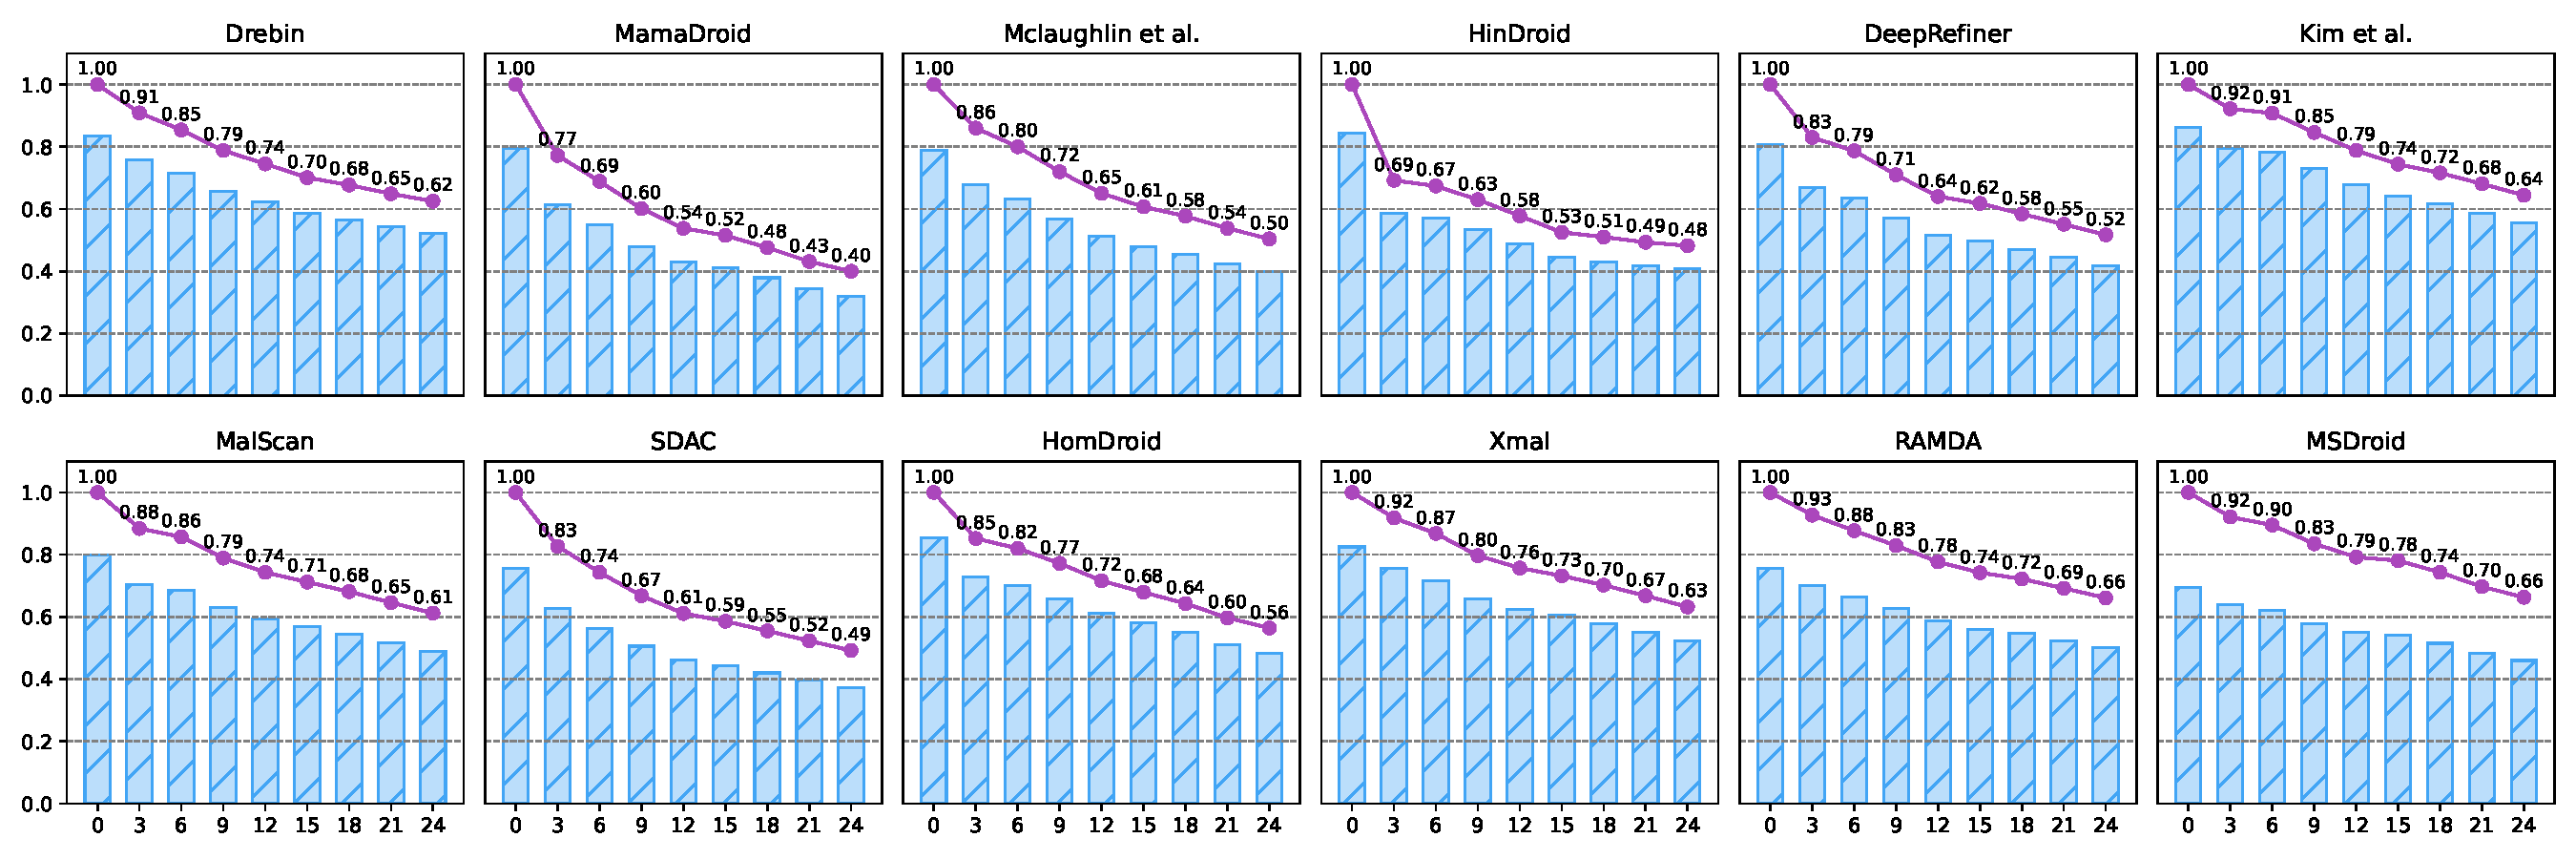
\includegraphics[width=\linewidth]{fig/evolution.pdf}
    %DIF <  \vspace{-0.1cm}
    %DIF >  \vspace{-0.2cm}
    \caption{The performance of the selected techniques against diverse malware evolution periods. Columns display the absolute values of $AUT(F1, N)$.
    The line charts depict the relative percentage of $AUT(F1, N)$ against $AUT(F1, 0)$.}
    \label{fig:evolution}
\DIFdelbeginFL %DIFDELCMD < \vspace{-0.3cm}
%DIFDELCMD < %%%
\DIFdelendFL \DIFaddbeginFL \vspace{-0.5cm}
\DIFaddendFL \end{figure*}

\bulletpoint{Malware evolution}
To quantify the impact of evolution on malware detectors, we utilize the $AUT(f, N)$~\cite{pendlebury2019tesseract}, where $f$ denotes the F1-score of a given approach, and $N$ represents the evolution period. 
The definition of $AUT(f, N)$ can be found in the Appendix~\ref{sub:aut}.
We set $N$ to 3, 6, 9, 12, 15, 18, 21, and 24 months in this experiment.
This metric ranges in (0, 1), where higher values indicate greater resilience to malware evolution.
In the study, we adopt a rolling algorithm over the data from 2011 to 2020 to calculate the $AUT(f, N)$.
Specifically, for each year, from 2011 to 2020, we first partition the data into training, validation, and testing sets with \texttt{8:1:1}.
Next, we train models with the training data, validate to get the best model, and evaluate it on the test set to get the F1-score as $AUT(F1, 0)$.
Then, the model is applied to test data in the next $N$ months, yielding $N$ F1-scores.
\DIFaddbegin \DIFadd{It is important to note that the $N$ months of test data may span across different years.
For example, if we use data from 2011 as the training set and set $N$ to 15 months, the corresponding test data will include apps collected from January 2012 to March 2013.
}\DIFaddend These scores are further used to calculate the $AUT(F1, N)$.
\DIFaddbegin \DIFadd{We repeat this process for each year from 2011 to 2020, resulting in ten distinct $AUT(F1, N)$ values for each $N$, if available.
For instance, when $N$ is 3 months, we can retrieve $AUT(F1, 3)$ values for each year from 2011 to 2019, since the test data for 3 months after training in 2020 is not available.
}\DIFaddend By averaging the $AUT(F1, N)$ values sourced from distinct yearly datasets, we chart the outcomes in Figure~\ref{fig:evolution}.

It is \DIFdelbegin \DIFdel{clear }\DIFdelend \DIFaddbegin \DIFadd{evident }\DIFaddend that malware evolution affects the effectiveness of \DIFdelbegin \DIFdel{these selected techniques}\DIFdelend \DIFaddbegin \DIFadd{the selected malware detectors}\DIFaddend .
This is \DIFdelbegin \DIFdel{within expectations, }\DIFdelend \DIFaddbegin \DIFadd{expected: }\DIFaddend as malware evolves over time, \DIFdelbegin \DIFdel{the semantics of malware }\DIFdelend \DIFaddbegin \DIFadd{its underlying semantics }\DIFaddend may change, making it \DIFdelbegin \DIFdel{harder }\DIFdelend \DIFaddbegin \DIFadd{more difficult }\DIFaddend for detectors to capture these \DIFdelbegin \DIFdel{changes.
Most DL approaches display superior resilience against malware evolution compared to their TML }\DIFdelend \DIFaddbegin \DIFadd{behaviors.
Overall, most DL-based approaches exhibit stronger resilience to malware evolution than their TML-based }\DIFaddend counterparts.
Specifically, the majority of DL techniques retain \DIFdelbegin \DIFdel{about }\DIFdelend \DIFaddbegin \DIFadd{around }\DIFaddend 60\% effectiveness even after two years\DIFdelbegin \DIFdel{. 
In contrast, }\DIFdelend \DIFaddbegin \DIFadd{, whereas }\DIFaddend many TML methods see their F1-scores \DIFdelbegin \DIFdel{reduced to }\DIFdelend \DIFaddbegin \DIFadd{drop to about }\DIFaddend 50\% \DIFdelbegin \DIFdel{within the same time span}\DIFdelend \DIFaddbegin \DIFadd{over the same period}\DIFaddend .
This disparity can be \DIFdelbegin \DIFdel{traced back }\DIFdelend \DIFaddbegin \DIFadd{attributed }\DIFaddend to the inherent capability of DL \DIFdelbegin \DIFdel{methods to discern intricate patterns , which TML might }\DIFdelend \DIFaddbegin \DIFadd{models to capture more intricate patterns that TML methods may }\DIFaddend miss.
Interestingly, \DIFdelbegin \DIFdel{Mclaughlin }\DIFdelend \DIFaddbegin \DIFadd{McLaughlin }\DIFaddend et al. and DeepRefiner \DIFdelbegin \DIFdel{, do not fare }\DIFdelend \DIFaddbegin \DIFadd{do not perform }\DIFaddend as well over time.
\DIFdelbegin \DIFdel{This could be attributed to }\DIFdelend \DIFaddbegin \DIFadd{A plausible reason is }\DIFaddend their reliance on \DIFdelbegin \DIFdel{apps' original }\DIFdelend \DIFaddbegin \DIFadd{raw }\DIFaddend bytecode as input, which may contain \DIFdelbegin \DIFdel{more }\DIFdelend \DIFaddbegin \DIFadd{substantial }\DIFaddend noise and complicate \DIFdelbegin \DIFdel{the semantic extractionprocess.
}\DIFdelend \DIFaddbegin \DIFadd{semantic extraction.
To enhance the robustness of ML-based Android malware detectors against malware evolution, two aspects are particularly important:
(i) extracting robust features that are less susceptible to temporal changes—for example, Xmal and RAMDA use carefully selected features (such as stable API calls and permissions) and tend to be more resilient to evolution;
and (ii) designing models that can effectively capture evolving malware semantics, such as persistent malicious behaviors—for instance, MsDroid employs a graph neural network to model structural relationships among code components, enabling it to better capture these evolving semantics.
}\DIFaddend 

\DIFdelbegin %DIFDELCMD < \begin{table}[t]
%DIFDELCMD <     %%%
\DIFdelendFL \DIFaddbeginFL \begin{figure*}[t]
    \DIFaddendFL \centering
    \DIFdelbeginFL %DIFDELCMD < \renewcommand{\arraystretch}{0.7}
%DIFDELCMD <     %%%
\DIFdelendFL \DIFaddbeginFL 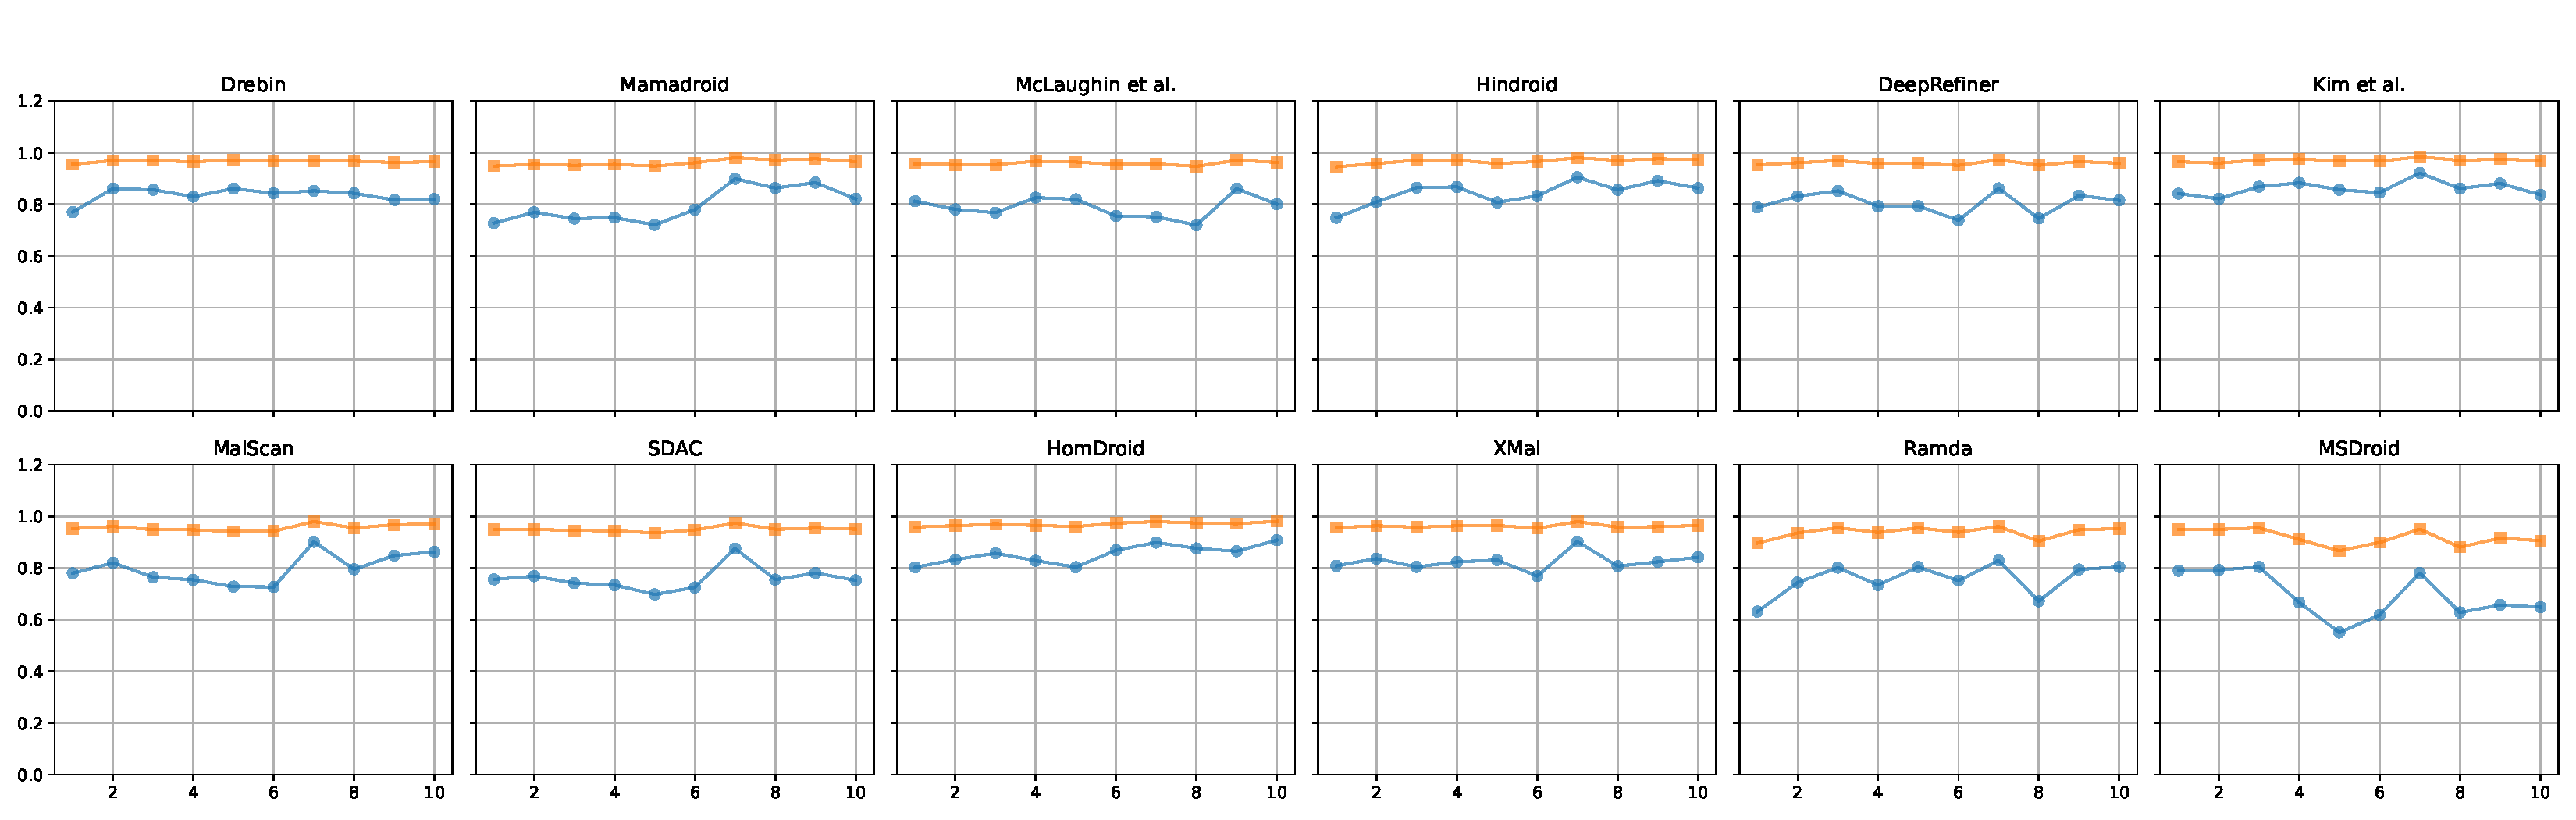
\includegraphics[width=0.94\linewidth]{fig/stable_trend.pdf}
    \vspace{-0.2cm}
    \DIFaddendFL \caption{\DIFdelbeginFL \DIFdelFL{The F-score }\DIFdelendFL \DIFaddbeginFL \DIFaddFL{Performance }\DIFaddendFL of the selected \DIFaddbeginFL \DIFaddFL{detection }\DIFaddendFL approaches \DIFdelbeginFL \DIFdelFL{under different obfuscation strategies~\mbox{%DIFAUXCMD
\cite{aonzo2020obfuscapk}}\hskip0pt%DIFAUXCMD
}\DIFdelendFL \DIFaddbeginFL \DIFaddFL{for each year from 2011 to 2020. Orange markers indicate Accuracy, and blue markers indicate F1-score}\DIFaddendFL .}
    %DIF <  \vspace{-0.1cm}
    \DIFdelbeginFL %DIFDELCMD < \begin{adjustbox}{width=0.74\linewidth, center}
%DIFDELCMD <     \begin{tabular}{@{}c|c|c|c|c|c@{}}
%DIFDELCMD <     \toprule
%DIFDELCMD <     \diagbox[innerleftsep=-0.1em, innerrightsep=-0.3em, height=2.7em,width=7em]{\textbf{Approach}}{\textbf{Obfuscation}} & %%%
\textbf{%DIFDELCMD < \begin{tabular}[c]{@{}c@{}}%%%
\DIFdelFL{Without }%DIFDELCMD < \\ %%%
\DIFdelFL{Obfus.}%DIFDELCMD < \end{tabular}%%%
} %DIFAUXCMD
%DIFDELCMD < & %%%
\textbf{%DIFDELCMD < \begin{tabular}[c]{@{}c@{}}%%%
\DIFdelFL{Rename }%DIFDELCMD < \\ %%%
\DIFdelFL{Identifier}%DIFDELCMD < \end{tabular}%%%
} %DIFAUXCMD
%DIFDELCMD < & %%%
\textbf{%DIFDELCMD < \begin{tabular}[c]{@{}c@{}}%%%
\DIFdelFL{Encrypt }%DIFDELCMD < \\ %%%
\DIFdelFL{Resource}%DIFDELCMD < \end{tabular}%%%
} %DIFAUXCMD
%DIFDELCMD < & %%%
\textbf{%DIFDELCMD < \begin{tabular}[c]{@{}c@{}}%%%
\DIFdelFL{Modify }%DIFDELCMD < \\ %%%
\DIFdelFL{Code}%DIFDELCMD < \end{tabular}%%%
} %DIFAUXCMD
%DIFDELCMD < & %%%
\textbf{%DIFDELCMD < \begin{tabular}[c]{@{}c@{}}%%%
\DIFdelFL{Reflect }%DIFDELCMD < \\ %%%
\DIFdelFL{Invocation}%DIFDELCMD < \end{tabular}%%%
} %DIFAUXCMD
%DIFDELCMD < \\ \midrule
%DIFDELCMD <     %%%
\DIFdelFL{Drebin      }%DIFDELCMD < & %%%
\DIFdelFL{0.732 }%DIFDELCMD < & %%%
\DIFdelFL{0.702 }%DIFDELCMD < & %%%
\DIFdelFL{0.701 }%DIFDELCMD < & %%%
\DIFdelFL{0.732 }%DIFDELCMD < & %%%
\DIFdelFL{0.732 }%DIFDELCMD < \\ \midrule
%DIFDELCMD <     %%%
\DIFdelFL{MamaDroid   }%DIFDELCMD < & %%%
\DIFdelFL{0.653 }%DIFDELCMD < & %%%
\DIFdelFL{0.274 }%DIFDELCMD < & %%%
\DIFdelFL{0.449 }%DIFDELCMD < & %%%
\DIFdelFL{0.150 }%DIFDELCMD < & %%%
\DIFdelFL{0.461 }%DIFDELCMD < \\ \midrule
%DIFDELCMD <     %%%
\DIFdelFL{Mclaughlin et al.
}%DIFDELCMD < & %%%
\DIFdelFL{0.750 }%DIFDELCMD < & %%%
\DIFdelFL{0.699 }%DIFDELCMD < & %%%
\DIFdelFL{0.722 }%DIFDELCMD < & %%%
\DIFdelFL{0.175 }%DIFDELCMD < & %%%
\DIFdelFL{0.727 }%DIFDELCMD < \\ \midrule
%DIFDELCMD <     %%%
\DIFdelFL{HinDroid    }%DIFDELCMD < & %%%
\DIFdelFL{0.750 }%DIFDELCMD < & %%%
\DIFdelFL{0.750 }%DIFDELCMD < & %%%
\DIFdelFL{0.741 }%DIFDELCMD < & %%%
\DIFdelFL{0.750 }%DIFDELCMD < & %%%
\DIFdelFL{0.735 }%DIFDELCMD < \\ \midrule
%DIFDELCMD <     %%%
\DIFdelFL{DeepRefiner }%DIFDELCMD < & %%%
\DIFdelFL{0.692 }%DIFDELCMD < & %%%
\DIFdelFL{0.618 }%DIFDELCMD < & %%%
\DIFdelFL{0.658 }%DIFDELCMD < & %%%
\DIFdelFL{0.297 }%DIFDELCMD < & %%%
\DIFdelFL{0.612 }%DIFDELCMD < \\ \midrule
%DIFDELCMD <     %%%
\DIFdelFL{Kim et al. 
}%DIFDELCMD < & %%%
\DIFdelFL{0.795 }%DIFDELCMD < & %%%
\DIFdelFL{0.795 }%DIFDELCMD < & %%%
\DIFdelFL{0.611 }%DIFDELCMD < & %%%
\DIFdelFL{0.795 }%DIFDELCMD < & %%%
\DIFdelFL{0.798 }%DIFDELCMD < \\ \midrule
%DIFDELCMD <     %%%
\DIFdelFL{MalScan     }%DIFDELCMD < & %%%
\DIFdelFL{0.675 }%DIFDELCMD < & %%%
\DIFdelFL{0.675 }%DIFDELCMD < & %%%
\DIFdelFL{0.675 }%DIFDELCMD < & %%%
\DIFdelFL{0.681 }%DIFDELCMD < & %%%
\DIFdelFL{0.687 }%DIFDELCMD < \\ \midrule
%DIFDELCMD <     %%%
\DIFdelFL{SDAC }%DIFDELCMD < & %%%
\DIFdelFL{0.563 }%DIFDELCMD < & %%%
\DIFdelFL{0.538 }%DIFDELCMD < & %%%
\DIFdelFL{0.552 }%DIFDELCMD < & %%%
\DIFdelFL{0.495 }%DIFDELCMD < & %%%
\DIFdelFL{0.552 }%DIFDELCMD < \\ \midrule
%DIFDELCMD <     %%%
\DIFdelFL{HomDroid    }%DIFDELCMD < & %%%
\DIFdelFL{0.729 }%DIFDELCMD < & %%%
\DIFdelFL{0.751 }%DIFDELCMD < & %%%
\DIFdelFL{0.706 }%DIFDELCMD < & %%%
\DIFdelFL{0.728 }%DIFDELCMD < & %%%
\DIFdelFL{0.739 }%DIFDELCMD < \\ \midrule
%DIFDELCMD <     %%%
\DIFdelFL{Xmal }%DIFDELCMD < & %%%
\DIFdelFL{0.727 }%DIFDELCMD < & %%%
\DIFdelFL{0.727 }%DIFDELCMD < & %%%
\DIFdelFL{0.727 }%DIFDELCMD < & %%%
\DIFdelFL{0.727 }%DIFDELCMD < & %%%
\DIFdelFL{0.727 }%DIFDELCMD < \\ \midrule
%DIFDELCMD <     %%%
\DIFdelFL{RAMDA}%DIFDELCMD < & %%%
\DIFdelFL{0.635 }%DIFDELCMD < & %%%
\DIFdelFL{0.635 }%DIFDELCMD < & %%%
\DIFdelFL{0.635 }%DIFDELCMD < & %%%
\DIFdelFL{0.635 }%DIFDELCMD < & %%%
\DIFdelFL{0.635 }%DIFDELCMD < \\ \midrule
%DIFDELCMD <     %%%
\DIFdelFL{MSDroid     }%DIFDELCMD < & %%%
\DIFdelFL{0.672 }%DIFDELCMD < & %%%
\DIFdelFL{0.675 }%DIFDELCMD < & %%%
\DIFdelFL{0.610 }%DIFDELCMD < & %%%
\DIFdelFL{0.356 }%DIFDELCMD < & %%%
\DIFdelFL{0.494 }%DIFDELCMD < \\ \bottomrule
%DIFDELCMD <     \end{tabular}
%DIFDELCMD <     \end{adjustbox}
%DIFDELCMD <     \label{table:res_obfuscation}
%DIFDELCMD <     \vspace{-0.3cm}
%DIFDELCMD < \end{table}
%DIFDELCMD < %%%
\DIFdelend \DIFaddbegin \label{fig:stable_trend}
\vspace{-0.5cm}
\end{figure*}
\DIFaddend 

\DIFaddbegin \bulletpoint{Detector stability on different time period datasets}
\DIFadd{Having examined the impact of malware evolution on detection effectiveness, we now turn to investigating whether the selected approaches can be applied to datasets collected in different time periods.
This experiment aims to assess the sensitivity of these approaches to temporal variations in the data. 
Such an analysis helps determine whether the approaches can be used reliably in practice and whether our findings are generalizable.
To cunduct this experiment, we partition the primary dataset into ten subsets based on the year of app collection, spanning from 2011 to 2020.
For each year-specific subset, we split the data into training (80\%), validation (10\%), and testing (10\%) sets.
Each approach is trained on the training set, with hyperparameters tuned using the validation set, and finally evaluated on the testing set.
}

\DIFadd{Figure~\ref{fig:stable_trend} illustrates the performance of the selected approaches across different years.
We observe that most approaches maintain relatively stable performance over time, indicating that they can be effectively applied to datasets collected at different periods.
This stability suggests that the approaches are generally applicable rather than tailored to specific datasets, which in turn supports the claim that our findings are likely to generalize across different time periods.
}



\DIFaddend \bulletpoint{Obfuscation}
Obfuscation techniques often alter an app's code. 
It can also affect the effectiveness of malware detectors~\cite{he2022msdroid}.
This part explores the influences of popular obfuscation techniques, \textit{i.e.,} renaming identifiers, encrypting resources, modifying code, and invoking reflection~\cite{aonzo2020obfuscapk}, on the selected approaches \DIFdelbegin \DIFdel{.
}%DIFDELCMD < 

%DIFDELCMD < %%%
\DIFdelend \DIFaddbegin \DIFadd{separately.
}\DIFaddend We apply the obfuscation strategies discussed earlier to the testing set in Table~\ref{tab:effectiveness_dataset}(\ding{182}).
Only the apps that can be successfully obfuscated by all the strategies are included in the obfuscated testing set, which contains 1,303 apps.
The effectiveness of the selected approaches, previously trained on the original training set, is then evaluated on this obfuscated testing set.
\DIFaddbegin 

\DIFaddend Table~\ref{table:res_obfuscation} summarizes the results.
\DIFdelbegin \DIFdel{Clearly}\DIFdelend \DIFaddbegin \DIFadd{Overall}\DIFaddend , most methods exhibit a \DIFdelbegin \DIFdel{performance decrease }\DIFdelend \DIFaddbegin \DIFadd{decrease in performance }\DIFaddend when subjected to obfuscation.
This is expected, as obfuscation can \DIFdelbegin \DIFdel{hidden the }\DIFdelend \DIFaddbegin \DIFadd{hide }\DIFaddend malicious semantics, making \DIFdelbegin \DIFdel{it harder }\DIFdelend \DIFaddbegin \DIFadd{them more difficult }\DIFaddend for detectors to capture\DIFdelbegin \DIFdel{them}\DIFdelend . 
Specifically, the impact of obfuscation on detectors significantly depends on how the detectors utilize APK features.
For instance, Xmal and RAMDA show greater robustness against obfuscation.
\DIFdelbegin \DIFdel{This is mainly because the employed obfuscation techniques do not change their used features }\DIFdelend \DIFaddbegin \DIFadd{A closer examination reveals that both approaches use API calls as features and rely on manually selected API calls as anchors, checking whether these APIs appear in the code.
We further observe that most of these anchor APIs are system APIs, which are less likely to be affected by the obfuscation techniques employed.
In other words, the obfuscation does not substantially modify the features used by these detectors}\DIFaddend .
In contrast, \DIFdelbegin \DIFdel{MamaDroid and MSDroid, relying on the }\DIFdelend \DIFaddbegin \DIFadd{approaches such as MamaDroid and MsDroid, which rely heavily on }\DIFaddend code structure, tend to be more susceptible to \DIFdelbegin \DIFdel{the }\DIFdelend code modification.
This suggests that the impact of obfuscation on detectors is closely related to the \DIFdelbegin \DIFdel{degree }\DIFdelend \DIFaddbegin \DIFadd{extent }\DIFaddend to which obfuscation techniques alter the semantics of the features \DIFdelbegin \DIFdel{utilized by the detectors.
Also, by }\DIFdelend \DIFaddbegin \DIFadd{they use.
Moreover, }\DIFaddend comparing MamaDroid and \DIFdelbegin \DIFdel{MSDroid --- both relying on the code structure --- we observe that a detector's robustness against }\DIFdelend \DIFaddbegin \DIFadd{MsDroid—both structure-based—indicates that robustness to }\DIFaddend obfuscation is also \DIFdelbegin \DIFdel{shaped }\DIFdelend \DIFaddbegin \DIFadd{influenced }\DIFaddend by the model's \DIFdelbegin \DIFdel{semantic extraction capability .
}\DIFdelend \DIFaddbegin \DIFadd{capability to extract semantics.
To better defend against obfuscation, it is therefore crucial to (i) select features that are less likely to be altered by obfuscation techniques and (ii) design models that can effectively extract the underlying semantics from these features.
}\DIFaddend 

\DIFaddbegin \begin{table}[t]
    \centering
    \renewcommand{\arraystretch}{0.9}
    \caption{\DIFaddFL{The F-score of the selected approaches under different obfuscation strategies~\mbox{%DIFAUXCMD
\cite{aonzo2020obfuscapk}}\hskip0pt%DIFAUXCMD
.}}
    %DIF >  \vspace{-0.1cm}
    \begin{adjustbox}{width=0.76\linewidth, center}
    \begin{tabular}{@{}c|c|c|c|c|c@{}}
    \toprule
    \diagbox[innerleftsep=-0.1em, innerrightsep=-0.3em, height=2.7em,width=7em]{\textbf{Approach}}{\textbf{Obfuscation}} & \textbf{\begin{tabular}[c]{@{}c@{}}\DIFaddFL{Without }\\ \DIFaddFL{Obfus.}\end{tabular}} & \textbf{\begin{tabular}[c]{@{}c@{}}\DIFaddFL{Rename }\\ \DIFaddFL{Identifier}\end{tabular}} & \textbf{\begin{tabular}[c]{@{}c@{}}\DIFaddFL{Encrypt }\\ \DIFaddFL{Resource}\end{tabular}} & \textbf{\begin{tabular}[c]{@{}c@{}}\DIFaddFL{Modify }\\ \DIFaddFL{Code}\end{tabular}} & \textbf{\begin{tabular}[c]{@{}c@{}}\DIFaddFL{Reflect }\\ \DIFaddFL{Invocation}\end{tabular}} \\ \midrule
    \DIFaddFL{Drebin      }& \DIFaddFL{0.732 }& \DIFaddFL{0.702 }& \DIFaddFL{0.701 }& \DIFaddFL{0.732 }& \DIFaddFL{0.732 }\\ \midrule
    \DIFaddFL{MamaDroid   }& \DIFaddFL{0.653 }& \DIFaddFL{0.274 }& \DIFaddFL{0.449 }& \DIFaddFL{0.150 }& \DIFaddFL{0.461 }\\ \midrule
    \DIFaddFL{Mclaughlin et al.  }& \DIFaddFL{0.750 }& \DIFaddFL{0.699 }& \DIFaddFL{0.722 }& \DIFaddFL{0.175 }& \DIFaddFL{0.727 }\\ \midrule
    \DIFaddFL{HinDroid    }& \DIFaddFL{0.750 }& \DIFaddFL{0.750 }& \DIFaddFL{0.741 }& \DIFaddFL{0.750 }& \DIFaddFL{0.735 }\\ \midrule
    \DIFaddFL{DeepRefiner }& \DIFaddFL{0.692 }& \DIFaddFL{0.618 }& \DIFaddFL{0.658 }& \DIFaddFL{0.297 }& \DIFaddFL{0.612 }\\ \midrule
    \DIFaddFL{Kim et al.  }& \DIFaddFL{0.795 }& \DIFaddFL{0.795 }& \DIFaddFL{0.611 }& \DIFaddFL{0.795 }& \DIFaddFL{0.798 }\\ \midrule
    \DIFaddFL{MalScan     }& \DIFaddFL{0.675 }& \DIFaddFL{0.675 }& \DIFaddFL{0.675 }& \DIFaddFL{0.681 }& \DIFaddFL{0.687 }\\ \midrule
    \DIFaddFL{SDAC }& \DIFaddFL{0.563 }& \DIFaddFL{0.538 }& \DIFaddFL{0.552 }& \DIFaddFL{0.495 }& \DIFaddFL{0.552 }\\ \midrule
    \DIFaddFL{HomDroid    }& \DIFaddFL{0.729 }& \DIFaddFL{0.751 }& \DIFaddFL{0.706 }& \DIFaddFL{0.728 }& \DIFaddFL{0.739 }\\ \midrule
    \DIFaddFL{Xmal }& \DIFaddFL{0.727 }& \DIFaddFL{0.727 }& \DIFaddFL{0.727 }& \DIFaddFL{0.727 }& \DIFaddFL{0.727 }\\ \midrule
    \DIFaddFL{RAMDA}& \DIFaddFL{0.635 }& \DIFaddFL{0.635 }& \DIFaddFL{0.635 }& \DIFaddFL{0.635 }& \DIFaddFL{0.635 }\\ \midrule
    \DIFaddFL{MSDroid     }& \DIFaddFL{0.672 }& \DIFaddFL{0.675 }& \DIFaddFL{0.610 }& \DIFaddFL{0.356 }& \DIFaddFL{0.494 }\\ \bottomrule
    \end{tabular}
    \end{adjustbox}
    \label{table:res_obfuscation}
    \vspace{-0.5cm}
\end{table}

\DIFaddend \bulletpoint{Adversarial attack}
We now utilize the dataset from Table~\ref{tab:effectiveness_dataset}(\ding{182}) to explore the impact of adversarial attacks on the performance of these selected approaches.
It is worth noting that we exclude approaches Mclaughlin et al. and DeepRefiner from this experiment.
This is because they truncate features at a certain size, making them easily bypassable.
Attackers can embed malicious code in the ignored part to evade detection.


% Mclaughlin et al. and DeepRefiner are excluded since they truncate features at a certain size, making them easily bypassable.
% Attackers can embed malicious code in the ignored part to evade detection.

To investigate the impact of adversarial attacks, we employ two primary strategies: Jacobian Saliency Map Attack (JSMA) and Randomized Input (RI).
These two techniques are chosen for their simplicity and effectiveness, compromising most ML-based malware detectors, as shown in Table~\ref{tab:adversarial}.
This suggests that more advanced attack strategies could pose even greater threats to these detectors~\cite{he2023efficient,zhao2021structural}.
For JSMA, we first train a substitute model with the training set, followed by applying JSMA to the model to generate adversarial samples.
\DIFaddbegin \DIFadd{Specifically, we utilize MLP as the substitute model for simple ML-based classifiers such as SVM, KNN, Random Forest, and MLP, for GNN-based detectors like MsDroid, we employ Graph Convolutional Networks (GCN) as the substitute model.
During the crafting of adversarial samples, we calculate the Jacobian matrix to identify the most influential features and iteratively modify them until the samples are misclassified by the target model or a maximum number of modifications is reached.
}\DIFaddend For RI, we randomly change a certain percentage of features in the testing set to produce adversarial examples.
When crafting adversarial samples, we follow~\cite{li2023black,chen2019android} to ensure the feature modifications are domain-mappable and can be repackaged to APKs.
For feature-vector-based approaches like Drebin, we follow~\cite{chen2019android} by constraining modifications to vector bits that are 0, changing them to 1.
This ensures that all required permissions and functions remain unchanged, keeping the app's functionality unaffected.
For graph-based solutions, we introduce non-disruptive modifications to the graph structures that do not alter the app's functionality.
The graph structure includes non-leaf nodes (user-defined functions) and leaf nodes (Android API). 
When adding a new edge, we select a non-leaf node in the graph and add a try block with a callee chosen from leaf nodes.
Since leaf nodes do not call any other nodes, the added edge does not affect the app's functionality.
% Taking Drebin as an example, we restrict our modifications to changing feature vectors from 0 to 1, keeping apps' functionalities unaffected.
To measure the robustness against adversarial attacks, we use two metrics from~\cite{li2023black}: Adversarial Success Rate (ASR) and Adversarial Perturbation Ratio (APR).
The detailed definitions can be found in the Appendix~\ref{sub:aut}.
Both metrics range (0, 1).
A higher ASR indicates increased vulnerability to adversarial attacks, while a higher APR suggests greater robustness against such attacks due to the model's ability to withstand perturbations.

By analyzing Table~\ref{tab:adversarial}, we note that JSMA yields an average ASR of 98.8\% across the evaluated approaches, indicating their vulnerability to such basic adversarial attacks, let alone more sophisticated ones~\cite{he2023efficient}.
The employed strategies are less effective on MamaDroid, HomDroid, and RAMDA.
The reason for MamaDroid and HomDroid could be linked to their abstraction of APKs' graph structures.
Interestingly, MamaDroid, HomDroid, and MalScan all utilize API calls and program graphs; the former two methods demonstrate greater resilience.
The key difference lies in their handling of program graphs --- MamaDroid abstracts these graphs using family and package names, and HomDroid employs social network triads for abstraction, in contrast to MalScan's direct use of the graphs.
These abstractions make the malicious semantics encoded in graph structures more resistant to perturbation, enhancing the robustness of the detectors built on them.
Additionally, RAMDA's resilience can be attributed to its customized Autoencoder, which learns compressed representations of benign apps, making it more defensive to adversarial examples.
These findings suggest that abstracting feature representations or augmenting models' defensive capabilities could improve malware detectors' robustness to adversarial attacks.

\begin{table}[t]
    \renewcommand{\arraystretch}{0.73}
    \caption{The robustness of our selected approaches on various adversarial attacks.}
    % \vspace{-0.1cm}
    \DIFdelbeginFL %DIFDELCMD < \begin{adjustbox}{width=0.7\linewidth, center}
%DIFDELCMD <  %%%
\DIFdelendFL \DIFaddbeginFL \begin{adjustbox}{width=0.9\linewidth, center}
 \DIFaddendFL \begin{tabular}{@{}c|cc|c||c|cc|c@{}}
  \toprule
  \multirow{2}{*}{\textbf{\makecell[c]{Selected\\ Approach}}} & \multicolumn{2}{c|}{\textbf{ASR}}      & \multirow{2}{*}{\textbf{APR}} & \multirow{2}{*}{\textbf{\makecell[c]{Selected\\ Approach}}} & \multicolumn{2}{c|}{\textbf{ASR}}      & \multirow{2}{*}{\textbf{APR}} \\ \cmidrule(lr){2-3} \cmidrule(lr){6-7}
   & \multicolumn{1}{c|}{\textbf{JSMA}} & \textbf{RI} &    &  & \multicolumn{1}{c|}{\textbf{JSMA}} & \textbf{RI} &    \\ \midrule
  Drebin  & \multicolumn{1}{c|}{1.000}  & 0.237& 0.001 & SDAC    & \multicolumn{1}{c|}{1.000}  & 0.146& 0.001 \\ \midrule
  MamaDroid  & \multicolumn{1}{c|}{0.972}  & 0.187& 0.021 & HomDroid& \multicolumn{1}{c|}{0.979}  & 0.303& 0.324 \\ \midrule
  HinDroid& \multicolumn{1}{c|}{1.000}  & 0.068& 0.004 & Xmal    & \multicolumn{1}{c|}{1.000}  & 0.142& 0.013 \\ \midrule
  Kim et al.  & \multicolumn{1}{c|}{1.000}  & 0.000& 0.004 & RAMDA   & \multicolumn{1}{c|}{0.931}  & 0.300& 0.023 \\ \midrule
  MalScan & \multicolumn{1}{c|}{1.000}  & 0.788& 0.001 & MSDroid & \multicolumn{1}{c|}{1.000}  & 0.022& 0.013 \\ \bottomrule
  \end{tabular}
    \end{adjustbox}
    \label{tab:adversarial}
\vspace{-0.3cm}
\end{table}

%DIF >  \begin{conclusionbox}
%DIF >      \textit{Summary:}
%DIF >      ML-based malware detectors are susceptible to various real-world challenges, including malware evolution, obfuscation, and adversarial attacks. \textit{Malware semantics} play a crucial role in determining the robustness of detectors against these challenges.
%DIF >  \end{conclusionbox}
\DIFaddbegin 


\DIFaddend \begin{conclusionbox}
    \textit{Summary:}
    ML-based malware detectors are \DIFdelbegin \DIFdel{susceptible to various }\DIFdelend \DIFaddbegin \DIFadd{inherently susceptible to }\DIFaddend real-world challenges \DIFdelbegin \DIFdel{, including }\DIFdelend \DIFaddbegin \DIFadd{such as }\DIFaddend malware evolution, \DIFaddbegin \DIFadd{code }\DIFaddend obfuscation, and adversarial attacks. \DIFdelbegin \textit{\DIFdel{Malware semantics}} %DIFAUXCMD
\DIFdel{play a crucial role in determining the robustness of detectors against }\DIFdelend \DIFaddbegin \DIFadd{Our findings suggest that detectors capable of capturing stable features and underlying malware semantics are more robust to }\DIFaddend these challenges. \DIFaddbegin \DIFadd{These observations highlight the need for future research to focus on identifying, modeling, and integrating semantically meaningful behavioral representations that remain invariant under transformation and evolution.
}\DIFaddend \end{conclusionbox}


% \vspace{-0.1cm}
\subsection{Efficiency}
\label{efficiency}
In this section, we scrutinize the efficiency of the selected methods across datasets from different years, 
focusing on \DIFdelbegin \DIFdel{both feature transformation }\DIFdelend \DIFaddbegin \DIFadd{the end-to-end efficiency of the entire detection pipeline, including feature extraction, transformation, }\DIFaddend and ML modeling.
For \DIFdelbegin \DIFdel{fairness, we normalize the time taken by these methods based on the analysis of }\DIFdelend \DIFaddbegin \DIFadd{feature extraction, we utilize average time for processing one APK and memory overhead during the extraction process.
For feature transformation, we measure the time taken to retrieve and encode the required features from pre-extracted features.
We normalize the time based on processing }\DIFaddend 20,000 apps per year.
\DIFaddbegin \DIFadd{For ML modeling, we evaluate the time taken for model training and prediction.
%DIF >  focusing on both feature transformation and ML modeling.
%DIF >  For fairness, we normalize the time taken by these methods based on the analysis of 20,000 apps per year.
}\DIFaddend All experiments are performed on a server with 32-core CPUs operating at 2.10 GHz, 251 GB of physical memory, and two GPUs, each with 32 GB of memory.

\DIFaddbegin \begin{figure}[t]
    \centering
    \begin{subfigure}{0.46\linewidth}
        \centering
        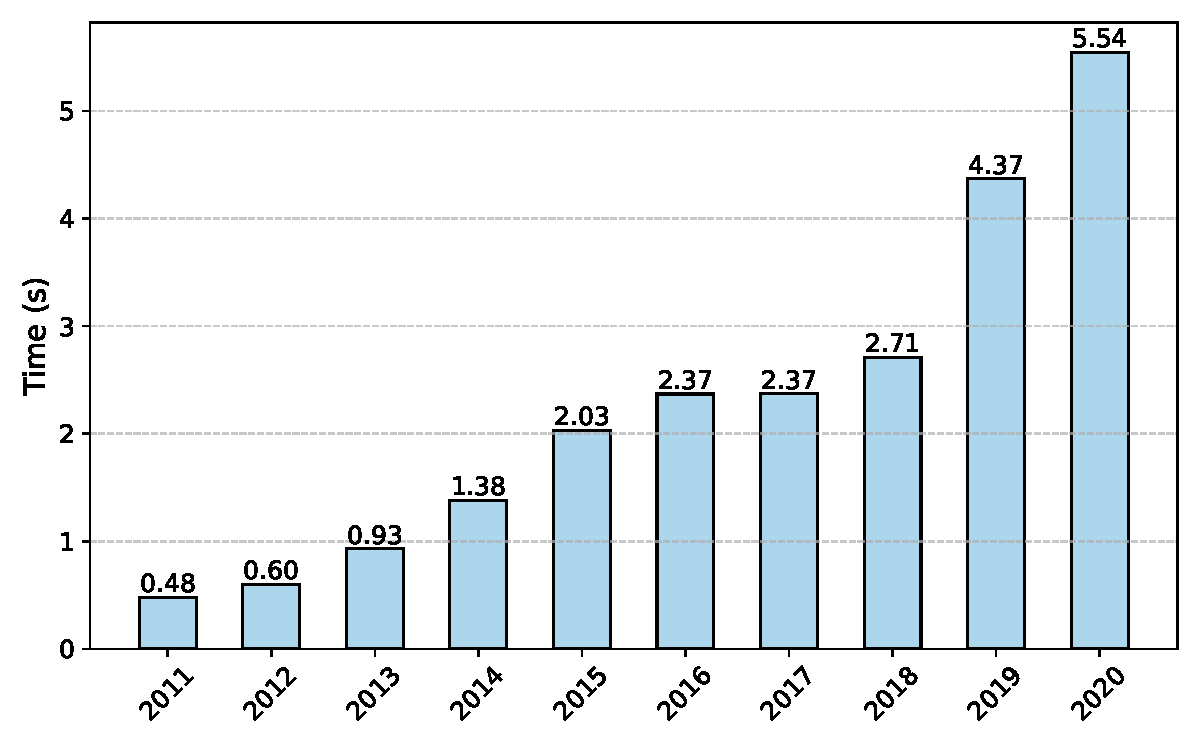
\includegraphics[width=\linewidth]{fig/efficiency_time.pdf}
        \caption{\DIFaddFL{Time efficiency}}
        \label{fig:efficiency_time}
    \end{subfigure}
    \begin{subfigure}{0.46\linewidth}
        \centering
        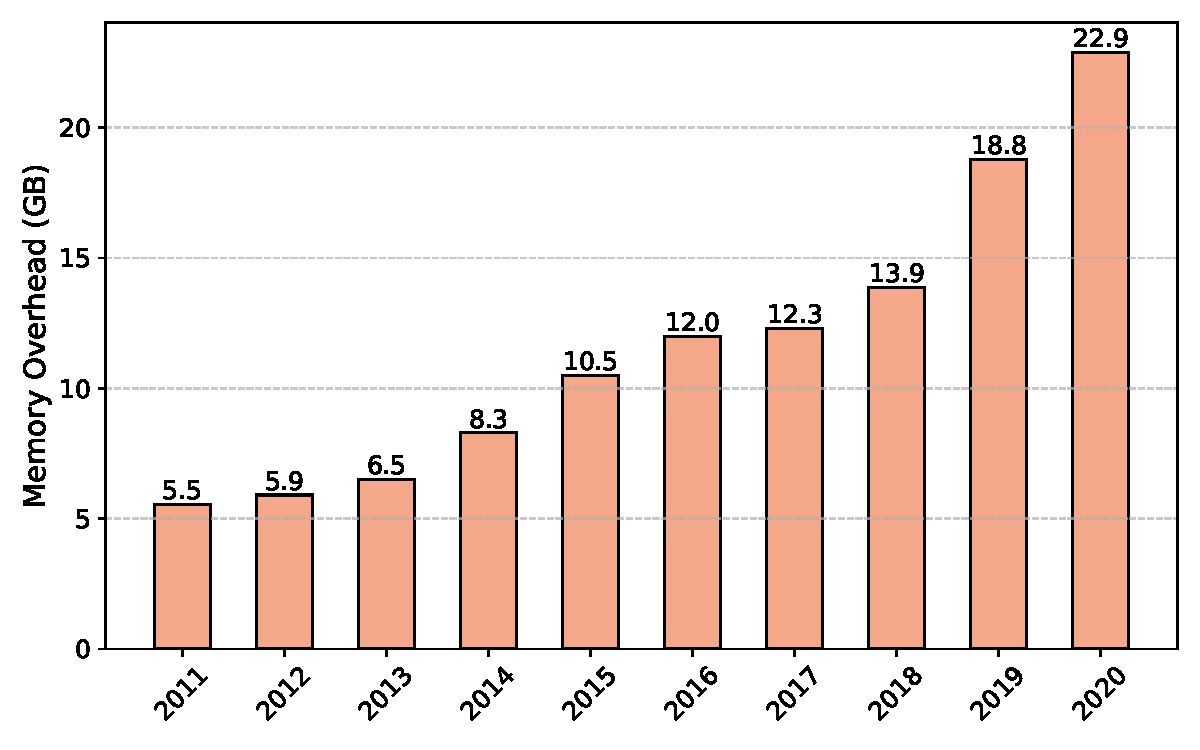
\includegraphics[width=\linewidth]{fig/memory_overhead.pdf}
        \caption{\DIFaddFL{Memory efficiency}}
        \label{fig:efficiency_memory}
    \end{subfigure}

    \caption{\DIFaddFL{The efficiency of extracting features from APKs in terms of time and memory.}}
    \label{fig:efficiency_combined}
    \vspace{-0.3cm}
\end{figure}


\begin{figure}[t]
    \centering
    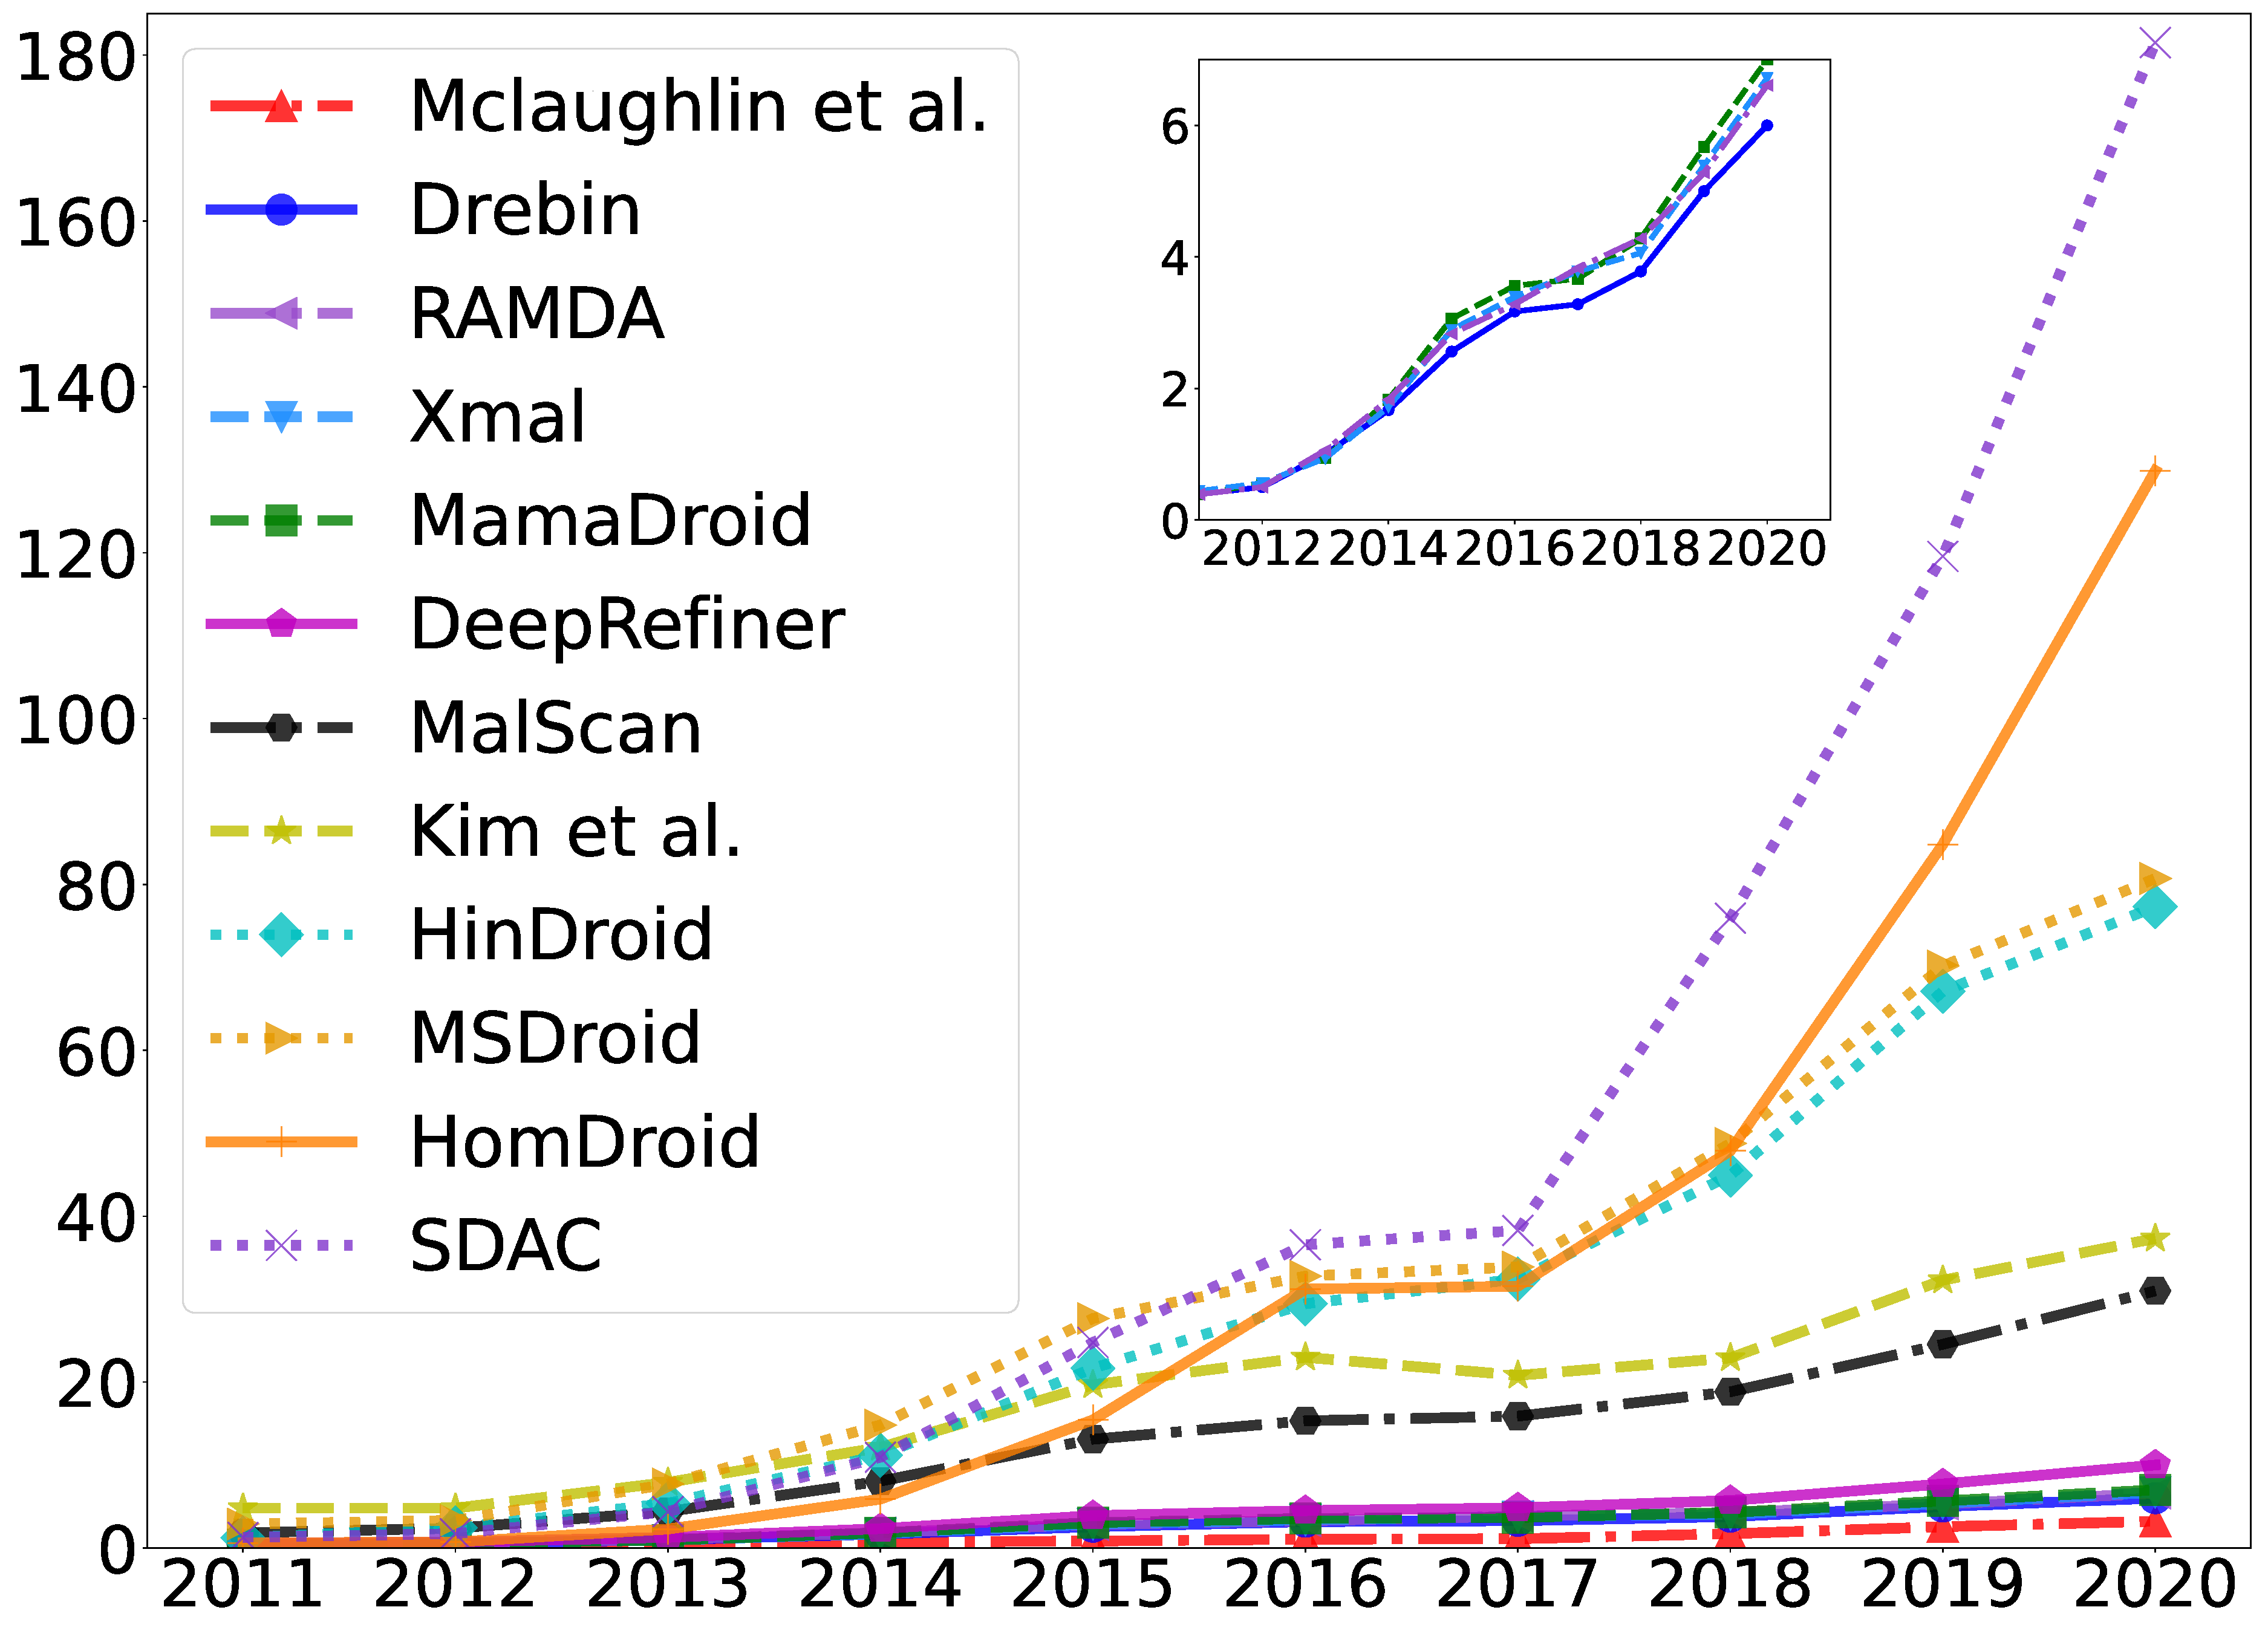
\includegraphics[width=0.61\linewidth]{fig/efficiency_encoding.pdf}
    \vspace{-0.2cm}
    \caption{\DIFaddFL{The efficiency of feature transformation of the selected approaches. The x-axis shows the dataset year, and the y-axis indicates the utilized time in hours.}}
    \label{fig:efficiency_encoding}
    \vspace{-0.3cm}
\end{figure}
\bulletpoint{Feature extraction}
\DIFadd{We first measure the performance overhead incurred during feature extraction from APKs.
The extraction process supports multi-process execution to enable concurrent feature extraction; in our experiments, we set the number of processes to 16.
We record the average time required to extract features from a single APK, as well as the average memory consumption.
Memory usage is monitored across all processes at 30-second intervals, and the mean value is reported as the memory overhead.
}

\DIFadd{Figure~\ref{fig:efficiency_combined} illustrates the time and memory efficiency of feature extraction. We observe that both time and memory overheads increase over the years, a trend that can be attributed to the growing complexity and size of APKs, which require more resources for effective feature extraction. In general, time and memory consumption are positively correlated, with higher extraction times typically accompanied by higher memory usage.
Despite this upward trend, the observed overheads remain acceptable for practical use of }\codename\DIFadd{. For example, extracting features from an APK released in 2020 takes approximately 5.5 seconds, with an overall memory consumption of about 22.9~GB when using 16 concurrent processes --- well within the capabilities of modern systems.
}

\begin{table*}[t]
    \centering
    \renewcommand{\arraystretch}{1.1}
    \caption{\DIFaddFL{The efficiency of selected approaches across datasets from different years, covering training and testing phases.}}
    \begin{adjustbox}{width=0.98\textwidth}
    \begin{tabular}{@{}cclc|c|c|c|c|c|c|c|c|c|c|c@{}}
    \cmidrule[\cmidrulewidth](l){4-15}
    \multicolumn{3}{c}{}   & \DIFaddFL{Drebin }& \DIFaddFL{MamaDroid }& \DIFaddFL{Mclaughlin et al. }& \DIFaddFL{HinDroid }& \DIFaddFL{DeepRefiner }& \DIFaddFL{Kim et al. }& \DIFaddFL{MalScan }& \DIFaddFL{SDAC }& \DIFaddFL{HomDroid }& \DIFaddFL{Xmal   }& \DIFaddFL{RAMDA }& \DIFaddFL{MSDroid }\\ \midrule
    \multicolumn{1}{c|}{\multirow{10}{*}{\raisebox{-2.8cm}{\rotatebox{90}{\textbf{\begin{tabular}[c]{@{}c@{}}Training\end{tabular}}}}}} & \multicolumn{2}{c|}{\textbf{\DIFaddFL{2011}}} & \DIFaddFL{15.11s  }& \DIFaddFL{1.90s }& \DIFaddFL{128m22s }& \DIFaddFL{2m19s }& \DIFaddFL{369m18s }& \DIFaddFL{98m47s }& \DIFaddFL{1m14s }& \DIFaddFL{84m47s }& \DIFaddFL{2.00s }& \DIFaddFL{1m15s  }& \DIFaddFL{1m6s }& \DIFaddFL{20m19s }\\ \cmidrule[\cmidrulewidth](lr){2-15}
    \multicolumn{1}{c|}{} & \multicolumn{2}{c|}{\textbf{\DIFaddFL{2012}}} & \DIFaddFL{20.88s  }& \DIFaddFL{1.94s }& \DIFaddFL{97m01s  }& \DIFaddFL{2m18s }& \DIFaddFL{359m35s   }& \DIFaddFL{92m47s  }& \DIFaddFL{1m18s   }& \DIFaddFL{89m05s   }& \DIFaddFL{2.04s     }& \DIFaddFL{1m25s  }& \DIFaddFL{1m11s }& \DIFaddFL{37m54s }\\ \cmidrule[\cmidrulewidth](lr){2-15}
    \multicolumn{1}{c|}{} & \multicolumn{2}{c|}{\textbf{\DIFaddFL{2013}}} & \DIFaddFL{22.37s  }& \DIFaddFL{2.12s }& \DIFaddFL{172m20s }& \DIFaddFL{2m13s }& \DIFaddFL{477m18s   }& \DIFaddFL{115m40s }& \DIFaddFL{1m24s   }& \DIFaddFL{115m35s  }& \DIFaddFL{2.04s     }& \DIFaddFL{50.36s }& \DIFaddFL{1m06s }& \DIFaddFL{40m11s }\\ \cmidrule[\cmidrulewidth](lr){2-15}
    \multicolumn{1}{c|}{} & \multicolumn{2}{c|}{\textbf{\DIFaddFL{2014}}} & \DIFaddFL{32.49s  }& \DIFaddFL{2.46s }& \DIFaddFL{128m13s }& \DIFaddFL{2m40s }& \DIFaddFL{629m26s   }& \DIFaddFL{104m03s }& \DIFaddFL{1m33s   }& \DIFaddFL{132m55s  }& \DIFaddFL{2.20s     }& \DIFaddFL{2m20s  }& \DIFaddFL{1m17s }& \DIFaddFL{42m07s }\\ \cmidrule[\cmidrulewidth](lr){2-15}
    \multicolumn{1}{c|}{} & \multicolumn{2}{c|}{\textbf{\DIFaddFL{2015}}} & \DIFaddFL{26.40s  }& \DIFaddFL{2.60s }& \DIFaddFL{411m03s }& \DIFaddFL{2m44s }& \DIFaddFL{730m41s   }& \DIFaddFL{115m27s }& \DIFaddFL{1m38s   }& \DIFaddFL{250m07s  }& \DIFaddFL{2.22s     }& \DIFaddFL{2m10s  }& \DIFaddFL{1m20s }& \DIFaddFL{42m52s }\\ \cmidrule[\cmidrulewidth](lr){2-15}
    \multicolumn{1}{c|}{} & \multicolumn{2}{c|}{\textbf{\DIFaddFL{2016}}} & \DIFaddFL{32.62s  }& \DIFaddFL{2.99s }& \DIFaddFL{234m19s }& \DIFaddFL{2m51s }& \DIFaddFL{867m25s   }& \DIFaddFL{135m50s }& \DIFaddFL{1m42s   }& \DIFaddFL{470m38s  }& \DIFaddFL{2.26s     }& \DIFaddFL{1m05s  }& \DIFaddFL{1m19s }& \DIFaddFL{142m23s }\\ \cmidrule[\cmidrulewidth](lr){2-15}
    \multicolumn{1}{c|}{} & \multicolumn{2}{c|}{\textbf{\DIFaddFL{2017}}} & \DIFaddFL{22.36s  }& \DIFaddFL{2.75s }& \DIFaddFL{192m41s }& \DIFaddFL{2m28s }& \DIFaddFL{997m04s   }& \DIFaddFL{145m24s }& \DIFaddFL{1m37s   }& \DIFaddFL{296m05s  }& \DIFaddFL{2.22s     }& \DIFaddFL{1m54s  }& \DIFaddFL{1m20s }& \DIFaddFL{47m22s }\\ \cmidrule[\cmidrulewidth](lr){2-15}
    \multicolumn{1}{c|}{} & \multicolumn{2}{c|}{\textbf{\DIFaddFL{2018}}} & \DIFaddFL{19.97s  }& \DIFaddFL{2.91s }& \DIFaddFL{227m48s }& \DIFaddFL{2m36s }& \DIFaddFL{933m12s   }& \DIFaddFL{128m32s }& \DIFaddFL{1m34s   }& \DIFaddFL{716m43s  }& \DIFaddFL{2.21s     }& \DIFaddFL{1m19s  }& \DIFaddFL{1m21s }& \DIFaddFL{155m50s }\\ \cmidrule[\cmidrulewidth](lr){2-15}
    \multicolumn{1}{c|}{} & \multicolumn{2}{c|}{\textbf{\DIFaddFL{2019}}} & \DIFaddFL{26.83s  }& \DIFaddFL{3.03s }& \DIFaddFL{514m18s }& \DIFaddFL{2m34s }& \DIFaddFL{968m50s   }& \DIFaddFL{185m43s }& \DIFaddFL{1m32s   }& \DIFaddFL{918m09s  }& \DIFaddFL{2.22s     }& \DIFaddFL{1m34s  }& \DIFaddFL{1m18s }& \DIFaddFL{130m41s }\\ \cmidrule[\cmidrulewidth](lr){2-15}
    \multicolumn{1}{c|}{} & \multicolumn{2}{c|}{\textbf{\DIFaddFL{2020}}} & \DIFaddFL{22.87s  }& \DIFaddFL{2.69s }& \DIFaddFL{771m44s }& \DIFaddFL{2m22s }& \DIFaddFL{1064m30s  }& \DIFaddFL{148m08s }& \DIFaddFL{1m29s   }& \DIFaddFL{867m55s  }& \DIFaddFL{2.17s     }& \DIFaddFL{2m09s  }& \DIFaddFL{1m12s }& \DIFaddFL{93m08s }\\ \midrule \midrule
    \multicolumn{1}{c|}{\multirow{10}{*}{\raisebox{-2cm}{\rotatebox{90}{\textbf{\begin{tabular}[c]{@{}c@{}}Testing\end{tabular}}}}}}  & \multicolumn{2}{c|}{\textbf{\DIFaddFL{2011}}} & \DIFaddFL{0.98s   }& \DIFaddFL{0.06s }& \DIFaddFL{16.03s  }& \DIFaddFL{29.82s }& \DIFaddFL{42.04s }& \DIFaddFL{0.62s }& \DIFaddFL{18.02s   }& \DIFaddFL{54.43s }& \DIFaddFL{1.20s     }& \DIFaddFL{0.32s   }& \DIFaddFL{0.07s  }& \DIFaddFL{4.33s    }\\ \cmidrule[\cmidrulewidth](lr){2-15}
    \multicolumn{1}{c|}{} & \multicolumn{2}{c|}{\textbf{\DIFaddFL{2012}}} & \DIFaddFL{1.36s   }& \DIFaddFL{0.06s }& \DIFaddFL{16.94s  }& \DIFaddFL{30.40s }& \DIFaddFL{45.50s }& \DIFaddFL{0.89s }& \DIFaddFL{22.23s   }& \DIFaddFL{53.97s  }& \DIFaddFL{1.30s  }& \DIFaddFL{0.32s   }& \DIFaddFL{0.07s  }& \DIFaddFL{6.15s   }\\ \cmidrule[\cmidrulewidth](lr){2-15}
    \multicolumn{1}{c|}{} & \multicolumn{2}{c|}{\textbf{\DIFaddFL{2013}}} & \DIFaddFL{1.48s   }& \DIFaddFL{0.06s }& \DIFaddFL{16.25s  }& \DIFaddFL{31.53s }& \DIFaddFL{50.36s }& \DIFaddFL{1.10s }& \DIFaddFL{19.27s   }& \DIFaddFL{1m21s   }& \DIFaddFL{1.22s  }& \DIFaddFL{0.34s   }& \DIFaddFL{0.07s  }& \DIFaddFL{7.14s   }\\ \cmidrule[\cmidrulewidth](lr){2-15}
    \multicolumn{1}{c|}{} & \multicolumn{2}{c|}{\textbf{\DIFaddFL{2014}}} & \DIFaddFL{1.53s   }& \DIFaddFL{0.06s }& \DIFaddFL{24.69s  }& \DIFaddFL{33.10s }& \DIFaddFL{59.22s }& \DIFaddFL{1.11s }& \DIFaddFL{24.83s   }& \DIFaddFL{1m51s   }& \DIFaddFL{1.36s  }& \DIFaddFL{0.32s   }& \DIFaddFL{0.09s  }& \DIFaddFL{11.29s  }\\ \cmidrule[\cmidrulewidth](lr){2-15}
    \multicolumn{1}{c|}{} & \multicolumn{2}{c|}{\textbf{\DIFaddFL{2015}}} & \DIFaddFL{1.73s   }& \DIFaddFL{0.06s }& \DIFaddFL{28.63s  }& \DIFaddFL{34.95s }& \DIFaddFL{1m12s  }& \DIFaddFL{0.97s }& \DIFaddFL{23.59s   }& \DIFaddFL{2m54s   }& \DIFaddFL{1.41s  }& \DIFaddFL{0.39s   }& \DIFaddFL{0.07s  }& \DIFaddFL{10.92s  }\\ \cmidrule[\cmidrulewidth](lr){2-15}
    \multicolumn{1}{c|}{} & \multicolumn{2}{c|}{\textbf{\DIFaddFL{2016}}} & \DIFaddFL{2.16s   }& \DIFaddFL{0.06s }& \DIFaddFL{40.04s  }& \DIFaddFL{36.50s }& \DIFaddFL{1m23s  }& \DIFaddFL{1.19s }& \DIFaddFL{23.92s   }& \DIFaddFL{3m37s   }& \DIFaddFL{1.54s  }& \DIFaddFL{0.33s   }& \DIFaddFL{0.08s  }& \DIFaddFL{18.72s  }\\ \cmidrule[\cmidrulewidth](lr){2-15}
    \multicolumn{1}{c|}{} & \multicolumn{2}{c|}{\textbf{\DIFaddFL{2017}}} & \DIFaddFL{1.46s   }& \DIFaddFL{0.06s }& \DIFaddFL{34.05s  }& \DIFaddFL{35.25s }& \DIFaddFL{1m12s  }& \DIFaddFL{0.92s }& \DIFaddFL{26.19s   }& \DIFaddFL{4m16s   }& \DIFaddFL{1.50s  }& \DIFaddFL{0.31s   }& \DIFaddFL{0.09s  }& \DIFaddFL{17.96s  }\\ \cmidrule[\cmidrulewidth](lr){2-15}
    \multicolumn{1}{c|}{} & \multicolumn{2}{c|}{\textbf{\DIFaddFL{2018}}} & \DIFaddFL{1.28s   }& \DIFaddFL{0.06s }& \DIFaddFL{36.39s  }& \DIFaddFL{35.17s }& \DIFaddFL{1m18s  }& \DIFaddFL{0.89s }& \DIFaddFL{22.67s   }& \DIFaddFL{6m21s   }& \DIFaddFL{1.28s  }& \DIFaddFL{0.32s   }& \DIFaddFL{0.09s  }& \DIFaddFL{17.96s  }\\ \cmidrule[\cmidrulewidth](lr){2-15}
    \multicolumn{1}{c|}{} & \multicolumn{2}{c|}{\textbf{\DIFaddFL{2019}}} & \DIFaddFL{1.74s   }& \DIFaddFL{0.06s }& \DIFaddFL{57.58s  }& \DIFaddFL{34.93s }& \DIFaddFL{1m33s  }& \DIFaddFL{1.18s }& \DIFaddFL{24.43s   }& \DIFaddFL{8m55s   }& \DIFaddFL{1.45s  }& \DIFaddFL{0.33s   }& \DIFaddFL{0.09s  }& \DIFaddFL{21.14s  }\\ \cmidrule[\cmidrulewidth](lr){2-15}
    \multicolumn{1}{c|}{} & \multicolumn{2}{c|}{\textbf{\DIFaddFL{2020}}} & \DIFaddFL{1.40s   }& \DIFaddFL{0.06s }& \DIFaddFL{1m12s   }& \DIFaddFL{33.90s }& \DIFaddFL{1m49s  }& \DIFaddFL{0.91s }& \DIFaddFL{23.62s   }& \DIFaddFL{8m27s   }& \DIFaddFL{1.52s  }& \DIFaddFL{0.41s   }& \DIFaddFL{0.07s  }& \DIFaddFL{19.54s  }\\ \bottomrule
    \end{tabular}
    \end{adjustbox}
    \label{tab:efficiency_ml_modeling}
\vspace{-0.3cm}
\end{table*}

\DIFaddend \bulletpoint{Feature transformation}
With \DIFdelbegin \DIFdel{the }\DIFdelend pre-extracted features \DIFdelbegin \DIFdel{, we assess }\DIFdelend \DIFaddbegin \DIFadd{available, we further evaluate }\DIFaddend the time efficiency of the selected methods in retrieving and encoding their required features. \DIFdelbegin \DIFdel{Note that we utilize }\DIFdelend \DIFaddbegin \DIFadd{All feature transformation procedures are executed using }\DIFaddend 16 \DIFdelbegin \DIFdel{processes to transform the features concurrently}\DIFdelend \DIFaddbegin \DIFadd{concurrent processes to ensure consistency across methods}\DIFaddend .

Figure~\ref{fig:efficiency_encoding} \DIFdelbegin \DIFdel{depicts the time taken by these approaches for }\DIFdelend \DIFaddbegin \DIFadd{presents the time overhead incurred by different approaches during }\DIFaddend feature transformation. \DIFdelbegin \DIFdel{As time advances, a noticeable increase in the timerequired for processing is evident, which aligns with the exponential growth in }\DIFdelend \DIFaddbegin \DIFadd{We observe a clear increasing trend over time, with more recent APKs requiring longer processing times. This trend is consistent with the rapid growth in both }\DIFaddend the size and \DIFdelbegin \DIFdel{complexity of APKs over the years. This observation underscores }\DIFdelend \DIFaddbegin \DIFadd{structural complexity of Android applications, which imposes higher computational costs during feature encoding. These results highlight }\DIFaddend the importance of designing \DIFdelbegin \DIFdel{efficient feature extraction }\DIFdelend \DIFaddbegin \DIFadd{scalable and efficient feature encoding }\DIFaddend strategies to keep pace with the \DIFdelbegin \DIFdel{rapid }\DIFdelend evolution of Android \DIFdelbegin \DIFdel{applications}\DIFdelend \DIFaddbegin \DIFadd{ecosystems}\DIFaddend .
Notably, \DIFdelbegin \DIFdel{there is a significant variance in the time consumption among different }\DIFdelend \DIFaddbegin \DIFadd{substantial variance in time consumption is observed across different detection }\DIFaddend approaches. This \DIFdelbegin \DIFdel{is within our expectation since various methods employ distinct features and encoding techniques. For instance, SDAC consumes the most time }\DIFdelend \DIFaddbegin \DIFadd{variation aligns with our expectations, as different methods rely on distinct feature types and encoding mechanisms with varying computational complexity. For example, SDAC exhibits the highest time overhead }\DIFaddend due to its \DIFdelbegin \DIFdel{requirement to query }\DIFdelend \DIFaddbegin \DIFadd{need to recursively traverse }\DIFaddend the program graph \DIFdelbegin \DIFdel{recursively for API call sequence generation. While methods like }\DIFdelend \DIFaddbegin \DIFadd{to generate API call sequences, an operation that scales poorly with increasing code complexity. In contrast, approaches such as }\DIFaddend Xmal and RAMDA are \DIFaddbegin \DIFadd{considerably }\DIFaddend more time-efficient, as they \DIFdelbegin \DIFdel{perform a one-time traversal on }\DIFdelend \DIFaddbegin \DIFadd{rely on a single traversal of }\DIFaddend the program graph to \DIFdelbegin \DIFdel{capture API calls}\DIFdelend \DIFaddbegin \DIFadd{extract API calls, resulting in significantly lower processing overhead}\DIFaddend .

\DIFaddbegin \DIFadd{Overall, these findings demonstrate that the choice of feature representation and encoding strategy has a substantial impact on time efficiency, underscoring a key trade-off between expressive feature modeling and computational scalability in ML-based Android malware detection.
}

\DIFaddend \bulletpoint{ML modeling}
For each yearly dataset, we \DIFdelbegin \DIFdel{divide it }\DIFdelend \DIFaddbegin \DIFadd{split the samples }\DIFaddend into training, validation, and testing sets \DIFdelbegin \DIFdel{with a ratio of }\DIFdelend \DIFaddbegin \DIFadd{using an }\DIFaddend \texttt{8:1:1} \DIFaddbegin \DIFadd{ratio}\DIFaddend . We then \DIFdelbegin \DIFdel{calculate }\DIFdelend \DIFaddbegin \DIFadd{measure }\DIFaddend the time required by the selected \DIFdelbegin \DIFdel{methods for }\DIFdelend \DIFaddbegin \DIFadd{approaches for both }\DIFaddend model training and testing. \DIFdelbegin \DIFdel{Note that we take the early stopping strategy during the training phase for DL models}\DIFdelend \DIFaddbegin \DIFadd{For deep learning (DL)-based methods, we adopt an early-stopping strategy during training to prevent overfitting and ensure fair comparison}\DIFaddend .

Table~\ref{tab:efficiency_ml_modeling} \DIFdelbegin \DIFdel{details the training time taken by these }\DIFdelend \DIFaddbegin \DIFadd{reports the training and testing time of the evaluated }\DIFaddend approaches.
From a \DIFdelbegin \DIFdel{horizontal }\DIFdelend \DIFaddbegin \DIFadd{cross-method }\DIFaddend perspective, we observe that most \DIFdelbegin \DIFdel{DL techniques require more time than their TMLcounterparts.
Furthermore, model }\DIFdelend \DIFaddbegin \DIFadd{DL-based techniques incur substantially higher training costs than traditional machine learning (TML) methods.
Moreover, training time is strongly correlated with model complexity, with deeper or more expressive architectures requiring longer training durations.
From a longitudinal perspective, training time consistently increases over the years, reflecting the growing }\DIFaddend complexity \DIFdelbegin \DIFdel{directly correlates with its training duration.
Analyzing longitudinally, there is a clear trend: as yearsprogress, the time requirements for these methods increase. 
This can be attributed to apps growing in complexity and an expanding feature set.
When combined with the effectiveness (Sec.}\DIFdelend \DIFaddbegin \DIFadd{of Android applications and the expanding dimensionality of extracted features.
When considered jointly with detection effectiveness (Section}\DIFaddend ~\ref{effectiveness}), \DIFdelbegin \DIFdel{we note that detection effectiveness does not always match resource utilization.
Striking a balance }\DIFdelend \DIFaddbegin \DIFadd{these results reveal that higher resource consumption does not necessarily translate into superior detection performance.
This observation highlights a fundamental trade-off }\DIFaddend between effectiveness and efficiency \DIFdelbegin \DIFdel{is critical when developing new detectors }\DIFdelend \DIFaddbegin \DIFadd{in ML-based Android malware detection.
Designing practical detectors therefore requires careful consideration of this balance, where incorporating semantically meaningful features plays a critical role in achieving strong performance without excessive computational overhead.
During the testing phase, we observe trends similar to those in training, with prediction time increasing modestly over time.
Nevertheless, most approaches are able to complete inference within seconds when evaluating approximately 2}\DIFaddend ,\DIFdelbegin \DIFdel{where semantics plays a key role in deciding the balance.
}\DIFdelend \DIFaddbegin \DIFadd{000 apps, indicating that they remain suitable for near real-time malware detection in practical deployment scenarios.
}\DIFaddend 








\DIFdelbegin %DIFDELCMD < \begin{figure}[t]
%DIFDELCMD <     \centering
%DIFDELCMD <     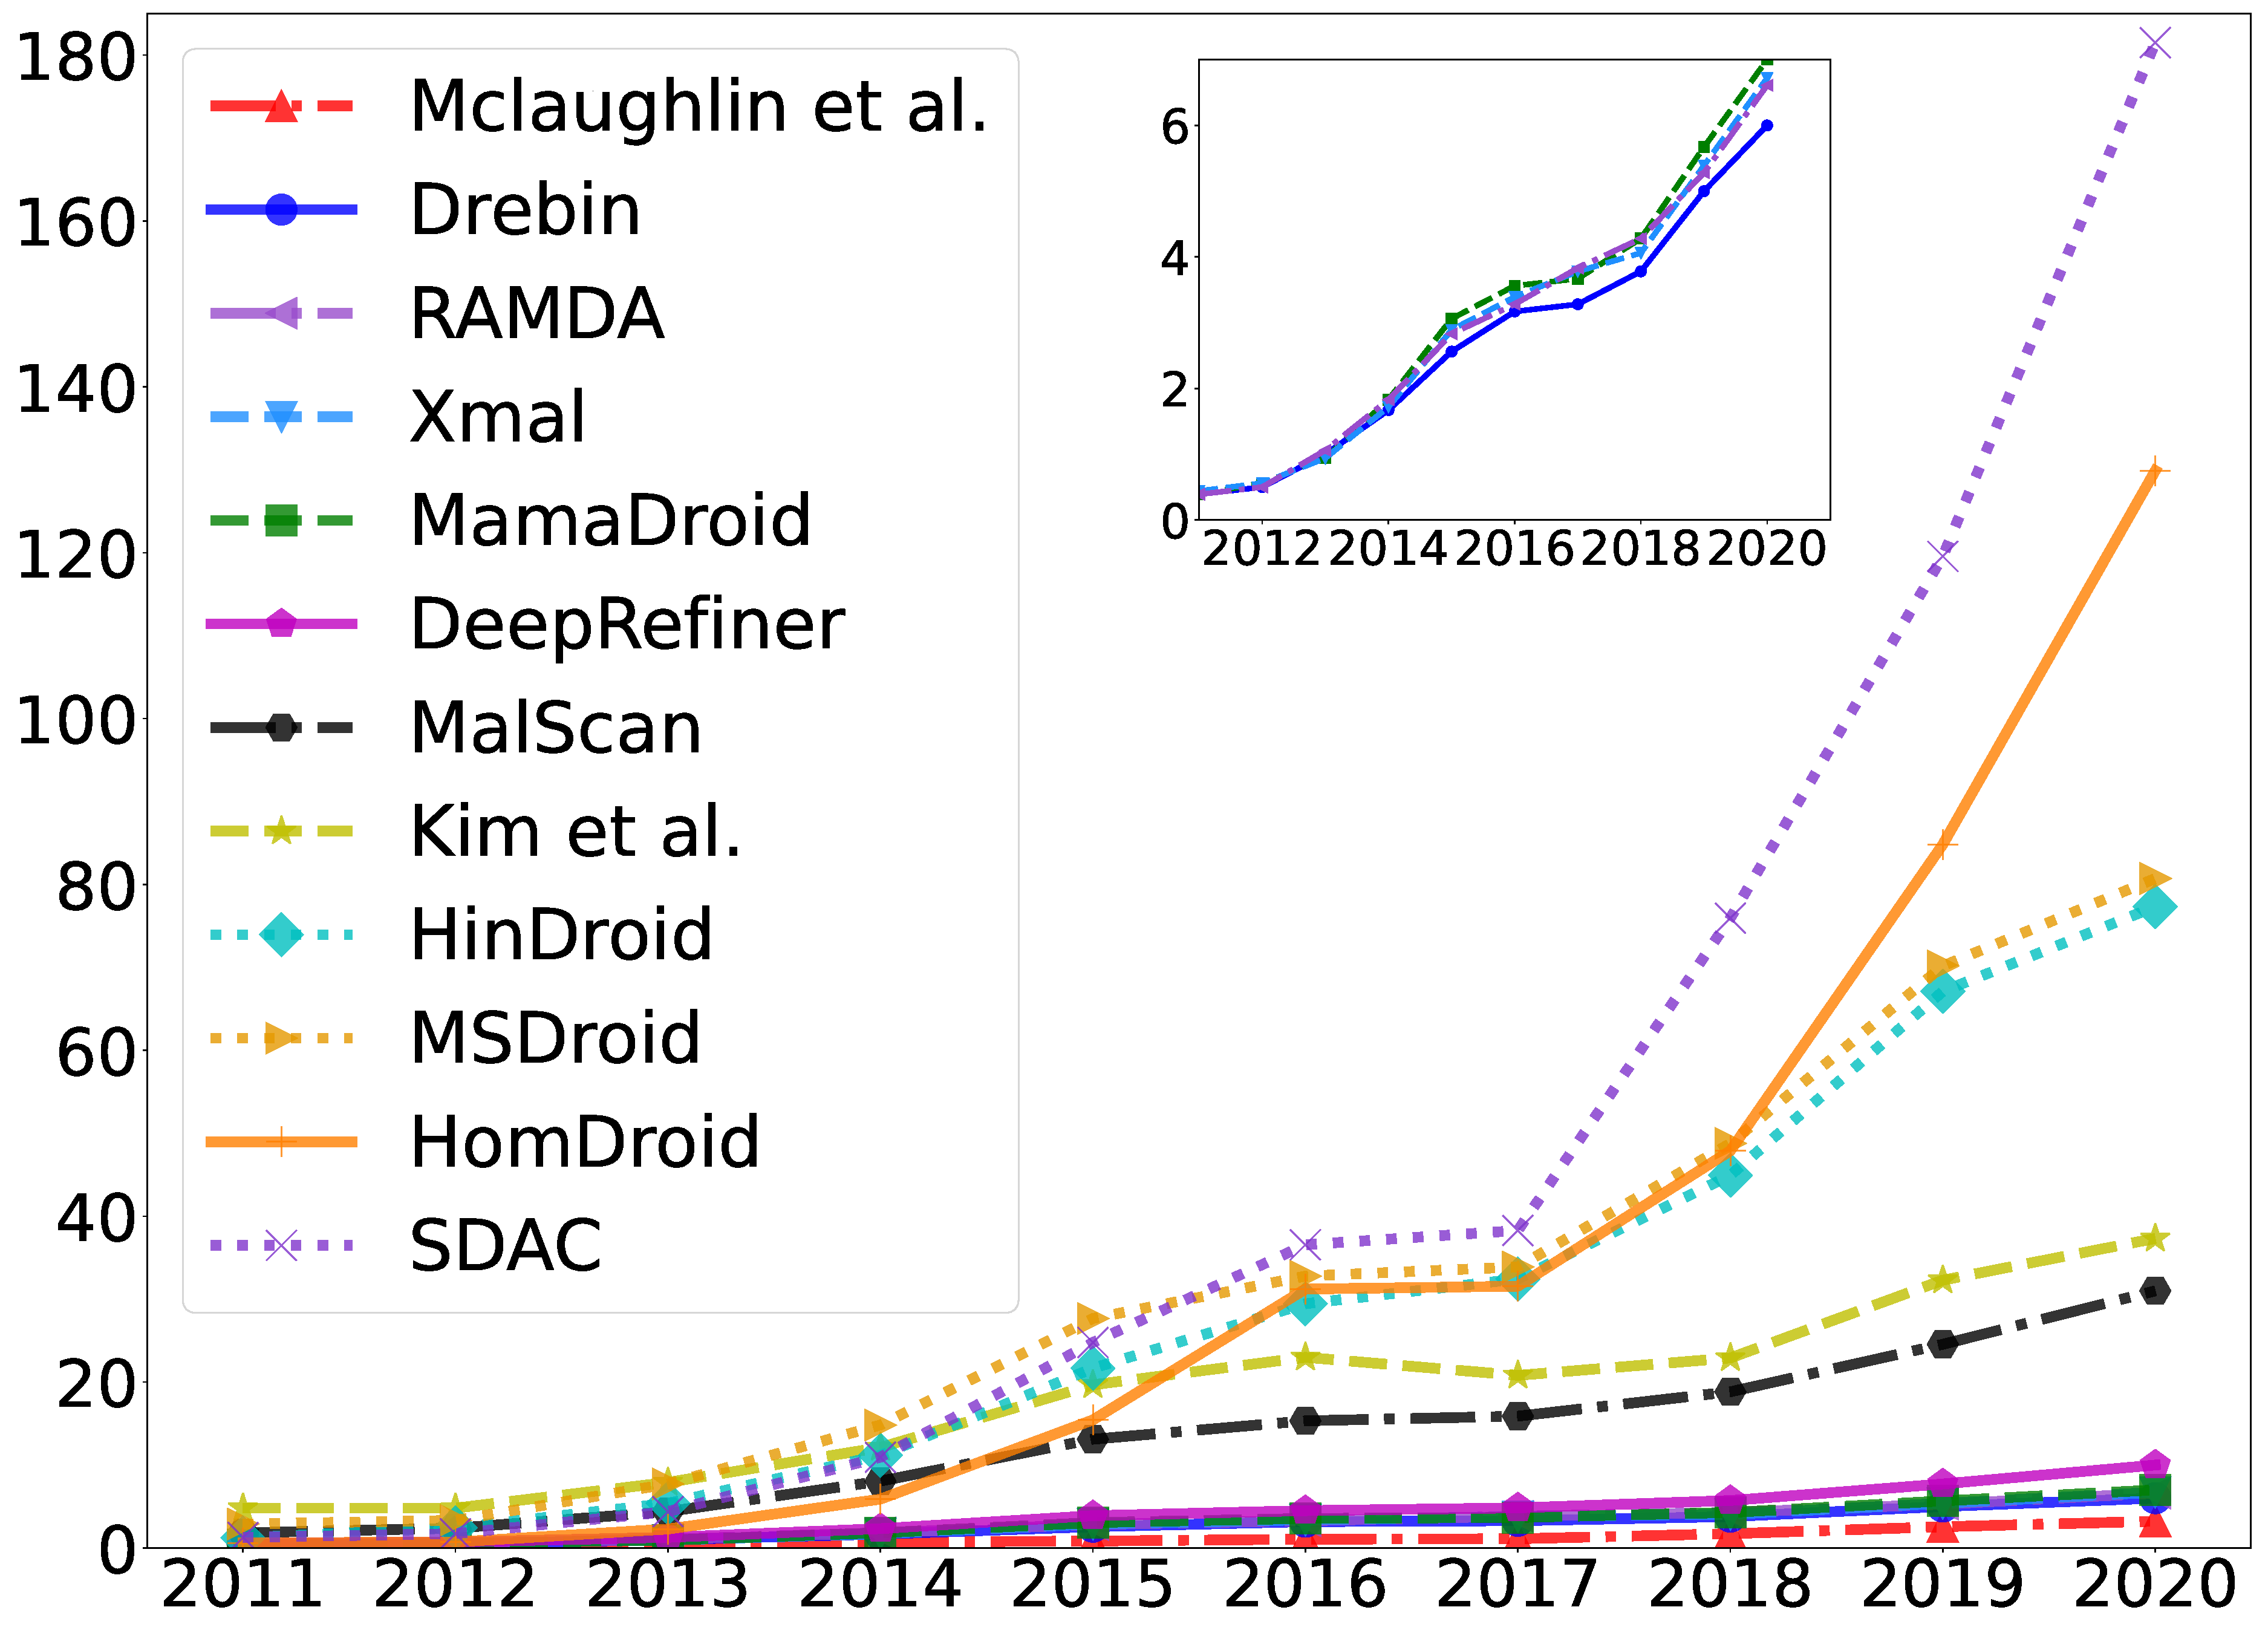
\includegraphics[width=0.56\linewidth]{fig/efficiency_encoding.pdf}
%DIFDELCMD <     %%%
%DIF <  \vspace{-0.2cm}
    %DIFDELCMD < \caption{%
{%DIFAUXCMD
\DIFdelFL{The efficiency of feature transformation of the selected approaches. The x-axis shows the dataset year, and the y-axis indicates the utilized time in hours.}}
    %DIFAUXCMD
%DIFDELCMD < \label{fig:efficiency_encoding}
%DIFDELCMD <     \vspace{-0.3cm}
%DIFDELCMD < \end{figure}
%DIFDELCMD < %%%
\DIFdelend %DIF >  \begin{conclusionbox}
%DIF >      \textit{Summary:}
%DIF >      The efficiency of ML-based malware detectors does not positively correlated with their effectiveness. Finding a balance between these two aspects is crucial when developing new detectors, requiring careful alignment of feature semantics with model capabilities to achieve an optimal trade-off.
%DIF >  \end{conclusionbox}

\begin{conclusionbox}
    \textit{Summary:}
    The \DIFdelbegin \DIFdel{efficiency of ML-based malware detectors does not positively correlated with their effectiveness. Finding a balance between these two aspects is crucial when developing new detectors, requiring careful alignment of feature semantics with model capabilities }\DIFdelend \DIFaddbegin \DIFadd{basic costs of feature extraction and malware prediction for ML-based detectors remain within acceptable limits for practical deployment. However, the primary efficiency bottleneck lies in feature transformation, where both what features are selected and how they are represented have a significant impact on encoding time. Notably, detector efficiency does not necessarily correlate with detection effectiveness, underscoring the importance of balancing effectiveness and efficiency.
    In particular, features should be well aligned with the capabilities of the chosen model }\DIFaddend to achieve an optimal trade-off. \DIFaddbegin \DIFadd{For example, when employing classifiers such as SVMs, extracting complex graph-based features may be unnecessary, as such models are not well suited to fully exploit the graph structure. Future work should focus on principled feature-model co-design, enabling efficient yet semantically expressive detection pipelines.
}\DIFaddend \end{conclusionbox}

%DIF <  \begin{center}
%DIF <      \begin{conclusionbox}
%DIF <      \textit{Takeaway:} 
%DIF <      When evaluating effectiveness and efficiency, performance does not always match resource use. It is crucial to find a balance when creating a new method.
%DIF <      \end{conclusionbox}
%DIF <  \end{center}
\DIFaddbegin \subsection{\DIFadd{Further Experimental Validation}}
\label{further_experiments}
\DIFaddend 





%DIF <  \subsection{Threats to Validity}
%DIF <  \label{Validity}
\DIFaddbegin \subsubsection{\textbf{\DIFadd{Influence of Reverse Engineering Tools}}}
\label{tool_influence}
\DIFadd{As discussed in Section~\ref{sub:compare}, different reverse engineering tools may extract divergent features from the same APK, potentially affecting the performance of ML-based malware detectors.
To systematically investigate this effect, we randomly select 4,000 apps from the additional dataset shown in Figure~\ref{fig:new_data}, maintaining a malware ratio of 10\%.
We then extract features using two widely adopted reverse engineering tools: Androguard~\mbox{%DIFAUXCMD
\cite{androguard} }\hskip0pt%DIFAUXCMD
and APKTool~\mbox{%DIFAUXCMD
\cite{apkt}}\hskip0pt%DIFAUXCMD
.
In this experiment, we focus on two commonly used feature types—API calls and permissions.
We split the dataset into training, validation, and testing sets, and train five representative ML models --- Random Forest, SVM, Decision Tree, KNN, and MLP --- using features extracted by each tool independently.
Each trained model is evaluated on its corresponding test set, and the results are compared to assess the impact of tool choice on detection performance.
}\DIFaddend 

%DIF <  \bulletpoint{Inconsistencies may exist between our evaluation results and the reported ones}
%DIF <  \jun{Please also highlight that our evaluation results may be inconsistent with the reported ones due to different biases. Future work should use our framework}
\DIFaddbegin \DIFadd{Our analysis reveals that the features extracted by the two tools are not always consistent.
In some cases, certain API calls or permissions are identified by one tool but missed by the other.
For instance, for the APK }\texttt{\DIFadd{00002EA4***0B6FB1}}\DIFadd{, Androguard extracts 15 additional API calls, such as }\texttt{\DIFadd{getRunningAppProcesses}} \DIFadd{and }\texttt{\DIFadd{getRunningTasks}}\DIFadd{, that are not detected by APKTool.
Such discrepancies are expected, as different tools employ distinct parsing strategies and static analysis techniques, leading to variations in feature coverage.
We further evaluate the performance of models trained on features extracted by each tool, with the results summarized in Table~\ref{tab:results}.
The results show noticeable performance differences across models depending on the tool used for feature extraction, demonstrating that the choice of reverse engineering tool can significantly influence experimental outcomes
This finding underscores the importance of standardizing the feature extraction toolchain when conducting comparative evaluations.
Accordingly, in this work, we use the same tool for all approaches to ensure fair and reproducible comparisons.
Given its consistently stronger performance across most settings, we select Androguard as the default feature extraction tool in }\codename\DIFadd{.
}\DIFaddend 

%DIF <  Inconsistencies might exist between our evaluation results and the reported ones due to different biases, such as datasets, feature extraction toolchains, and learning frameworks.
%DIF <  Our general-purpose framework aims to mitigate these biases and provide a fair comparison across various approaches for future research.
%DIF <  Specifically, we adopt standardized techniques across all tasks, including feature extraction and learning frameworks.
%DIF <  We also incorporate many evaluation scenarios, such as training data sizes, time decay, adversarial attacks, and efficiency, to ensure a comprehensive and accurate measurement using our crafted dataset.
%DIF <  % All the code and data of our framework will be released.
%DIF <  It is our hope that the framework can serve as a cornerstone for future work in ML-based Android malware detection.
\DIFaddbegin \begin{table}[t]
\centering
\caption{\DIFaddFL{Test Set Performance Comparison: APKTool vs Androguard Features}}
\label{tab:results}
\renewcommand{\arraystretch}{1.1}
\begin{adjustbox}{width=0.93\linewidth}
\begin{tabular}{l|cccc|cccc}
\hline
\multirow{2}{*}{\textbf{Model}} & \multicolumn{4}{c|}{\textbf{\DIFaddFL{APKTool}}} & \multicolumn{4}{c}{\textbf{\DIFaddFL{Androguard}}} \\
\cline{2-9}
& \textbf{\DIFaddFL{Acc.}} & \textbf{\DIFaddFL{Prec.}} & \textbf{\DIFaddFL{Rec.}} & \textbf{\DIFaddFL{F1}} & \textbf{\DIFaddFL{Acc.}} & \textbf{\DIFaddFL{Prec.}} & \textbf{\DIFaddFL{Rec.}} & \textbf{\DIFaddFL{F1}} \\
\hline
\DIFaddFL{RandomForest }& \DIFaddFL{0.975 }& \DIFaddFL{0.941 }& \DIFaddFL{0.800 }& \DIFaddFL{0.865 }& \DIFaddFL{0.984 }& \DIFaddFL{0.886 }& \DIFaddFL{0.975 }& \DIFaddFL{0.929 }\\
\DIFaddFL{SVM          }& \DIFaddFL{0.963 }& \DIFaddFL{0.931 }& \DIFaddFL{0.675 }& \DIFaddFL{0.783 }& \DIFaddFL{0.978 }& \DIFaddFL{0.921 }& \DIFaddFL{0.875 }& \DIFaddFL{0.897 }\\
\DIFaddFL{DecisionTree }& \DIFaddFL{0.960 }& \DIFaddFL{0.786 }& \DIFaddFL{0.825 }& \DIFaddFL{0.805 }& \DIFaddFL{0.984 }& \DIFaddFL{0.905 }& \DIFaddFL{0.950 }& \DIFaddFL{0.927 }\\
\DIFaddFL{KNN          }& \DIFaddFL{0.960 }& \DIFaddFL{0.900 }& \DIFaddFL{0.675 }& \DIFaddFL{0.771 }& \DIFaddFL{0.973 }& \DIFaddFL{0.941 }& \DIFaddFL{0.800 }& \DIFaddFL{0.865 }\\
\DIFaddFL{MLP          }& \DIFaddFL{0.973 }& \DIFaddFL{0.939 }& \DIFaddFL{0.775 }& \DIFaddFL{0.849 }& \DIFaddFL{0.981 }& \DIFaddFL{0.884 }& \DIFaddFL{0.950 }& \DIFaddFL{0.916 }\\
\hline
\end{tabular}
\end{adjustbox}
\vspace{-0.5cm}
\end{table}
\DIFaddend 

\DIFaddbegin \subsubsection{\textbf{\DIFadd{Detection Effectiveness}}}
\label{sec:detect_effectiveness}
\DIFadd{As described in Section~\ref{sec:dataset}, we use the primary dataset spanning 2011-2020 as the main benchmark for evaluating the effectiveness of the selected representative approaches, providing a comprehensive view of the state of ML-based Android malware detection.
To further validate the generalizability of our findings and examine whether they remain valid on more recent data, we conduct an additional evaluation using a supplementary dataset collected between 2021 and 2024, as illustrated in Figure~\ref{fig:new_data}.
For consistency, we split the dataset into training, validation, and testing sets using an }\texttt{\DIFadd{8:1:1}} \DIFadd{ratio, while maintaining a goodware-to-malware ratio of 9:1, following the same experimental setup as in Section~\ref{effectiveness}.
}

\DIFadd{Table~\ref{tab:2021_2024_results} reports the F1-score and accuracy of the selected approaches on the additional datasets.
We observe trends consistent with those obtained from the primary dataset: under realistic settings, Hindroid, Kim et al., and Homdroid consistently outperform other methods and achieve comparable F1-score and accuracy.
These results indicate that traditional machine learning (TML)-based and deep learning (DL)-based approaches continue to exhibit similar effectiveness on recent data, further supporting our earlier finding that DL-based methods may require a larger volume of malware samples to effectively distill malicious semantics and surpass TML-based approaches.
}

\DIFadd{This experiment serves as a lightweight yet fundamental validation that the selected representative approaches—and our key observations—remain effective on more recent datasets.
Other aspects of detector behavior, such as robustness and efficiency, are less sensitive to dataset time periods and therefore are not re-evaluated on the additional dataset.
Further discussion on the influence of dataset temporal characteristics is provided in Section~\ref{sec:discussion}.
}


\begin{table}[t]
\centering
\caption{\DIFaddFL{Average F1-Score and Accuracy for different methods on the additional datasets from 2021 to 2024.}}
\begin{adjustbox}{width=0.89\linewidth}
\begin{tabular}{lcccccc}
	\toprule
	\textbf{\DIFaddFL{Method}} & \DIFaddFL{Drebin }& \DIFaddFL{Mamadroid }& \DIFaddFL{Mclaughin et al. }& \DIFaddFL{Hindroid }& \DIFaddFL{DeepRefiner }& \DIFaddFL{Kim et al. }\\
\midrule
	\textbf{\DIFaddFL{F1-Score}} & \DIFaddFL{0.857 }& \DIFaddFL{0.716 }& \DIFaddFL{0.717 }& \DIFaddFL{0.900 }& \DIFaddFL{0.707 }& \DIFaddFL{0.879 }\\
	\textbf{\DIFaddFL{Accuracy}} & \DIFaddFL{0.973 }& \DIFaddFL{0.744 }& \DIFaddFL{0.744 }& \DIFaddFL{0.981 }& \DIFaddFL{0.742 }& \DIFaddFL{0.977 }\\
\midrule
\midrule
	\textbf{\DIFaddFL{Method}} & \DIFaddFL{Malscan }& \DIFaddFL{SDAC }& \DIFaddFL{Homdroid }& \DIFaddFL{Xmal }& \DIFaddFL{RAMDA }& \DIFaddFL{MsDroid }\\
\midrule
	\textbf{\DIFaddFL{F1-Score}} & \DIFaddFL{0.716 }& \DIFaddFL{0.735 }& \DIFaddFL{0.888 }& \DIFaddFL{0.670 }& \DIFaddFL{0.723 }& \DIFaddFL{0.823 }\\
	\textbf{\DIFaddFL{Accuracy}} & \DIFaddFL{0.743 }& \DIFaddFL{0.747 }& \DIFaddFL{0.979 }& \DIFaddFL{0.734 }& \DIFaddFL{0.932 }& \DIFaddFL{0.958 }\\
\bottomrule
\end{tabular}
\end{adjustbox}
\label{tab:2021_2024_results}
\end{table}




\DIFaddend % \vspace{-0.1cm}
\section{Findings and Recommendations}
\label{sec:findings}
We now draw from our findings to discuss the current state of ML-based Android malware detection and put forth recommendations to guide future research in this area.

% \subsection{Findings}
% \label{sec:findings}
\bulletpoint{Findings}
We summarize our key findings as follows:

\noindent \textit{(1) Current ML-based Android malware detectors still face open challenges.}
While ML models have been evidently effective in detecting malware~\cite{he2022msdroid,kim2018multimodal,li2021robust,mariconti2016mamadroid}, their effectiveness is still far from satisfactory when faced with challenging scenarios such as limited data size, rapid malware evolution, and adversarial attacks.

\noindent \textit{(2) Selecting features relevant to malware semantics is crucial for effective detection.}
\DIFdelbegin \DIFdel{Diverse }\DIFdelend \DIFaddbegin \DIFadd{A wide range of }\DIFaddend APK features, such as permissions and intents, have been leveraged \DIFdelbegin \DIFdel{to identify malware }\DIFdelend \DIFaddbegin \DIFadd{for malware detection}\DIFaddend ~\cite{xu2018deeprefiner,arp2014drebin,kim2018multimodal}.
These features \DIFdelbegin \DIFdel{profile apps }\DIFdelend \DIFaddbegin \DIFadd{serve to profile app behavior }\DIFaddend and play a \DIFdelbegin \DIFdel{pivotal role in shaping the effectivenessof malware detectors}\DIFdelend \DIFaddbegin \DIFadd{critical role in determining detector effectiveness}\DIFaddend .
Our findings \DIFdelbegin \DIFdel{indicate }\DIFdelend \DIFaddbegin \DIFadd{suggest }\DIFaddend that heuristic feature selection can \DIFdelbegin \DIFdel{help }\DIFdelend \DIFaddbegin \DIFadd{effectively }\DIFaddend reduce noise in the feature space, \DIFdelbegin \DIFdel{enabling models to }\DIFdelend \DIFaddbegin \DIFadd{allowing models to more readily }\DIFaddend identify malicious patterns \DIFdelbegin \DIFdel{more effectively, particularly in scenarios with limited data}\DIFdelend \DIFaddbegin \DIFadd{--- particularly in data-scarce settings}\DIFaddend .
However, we also observe that the semantics \DIFdelbegin \DIFdel{of various features }\DIFdelend \DIFaddbegin \DIFadd{captured by different feature types }\DIFaddend are not always complementary, and \DIFdelbegin \DIFdel{how to combine them does not be well explored.
Simply }\DIFdelend \DIFaddbegin \DIFadd{principled strategies for combining them remain underexplored.
Consequently, naively }\DIFaddend incorporating additional features does not necessarily \DIFdelbegin \DIFdel{lead to improved }\DIFdelend \DIFaddbegin \DIFadd{yield improved detection }\DIFaddend performance.

% Our analysis reveals that feature engineering helps models to discern malicious patterns when data is limited.
% However, including more features randomly does not guarantee enhanced performance. 
% Thus, researchers should carefully select features to improve the effectiveness and efficiency.
\noindent \textit{(3) More complex models are not a silver bullet in designing malware detectors.}
The literature reflects the trend towards employing more powerful ML models to detect malware~\cite{xu2018deeprefiner,arp2014drebin}.
Our analysis reveals that DL-based methods appear to be more resilient than TML-based approaches in adapting to malware evolution.
However, we also find that DL-based approaches are less effective than TML-based methods when the malware-to-goodware ratio is low.
This suggests that utilizing more complex models is not a universal solution for malware detection.
Instead, the choice of models should take into account the richness of the semantic information derived from the features.
\DIFaddbegin \DIFadd{One more practical observation is given feature sets including discrete features (}\textit{\DIFadd{i.e.,}} \DIFadd{permissions and API calls), ensembling models and DL models with embedding layers tend to outperform other typical models.
}


\DIFaddend % When introducing a new model to detect malware, it is crucial to justify the rationale behind it.

\noindent \textit{(4) Both feature abstraction and models' defensive mechanism contribute to detectors' robustness.}
Our analysis indicates that \DIFdelbegin \DIFdel{abstracting features can help models capture }\DIFdelend \DIFaddbegin \DIFadd{feature abstraction can help ML models capture more }\DIFaddend robust malicious patterns~\cite{bhagoji2018enhancing}.
For \DIFdelbegin \DIFdel{instance}\DIFdelend \DIFaddbegin \DIFadd{example}\DIFaddend , MamaDroid~\cite{mariconti2016mamadroid} abstracts program graphs \DIFdelbegin \DIFdel{with families and packages, enhancing its robustness to }\DIFdelend \DIFaddbegin \DIFadd{at the family and package levels, which enhances its robustness against }\DIFaddend adversarial attacks.
\DIFdelbegin \DIFdel{Moreover, bolstering the defensive capability }\DIFdelend \DIFaddbegin \DIFadd{In addition, strengthening the defensive capabilities }\DIFaddend of ML models can further \DIFdelbegin \DIFdel{amplify detectors' }\DIFdelend \DIFaddbegin \DIFadd{improve detector }\DIFaddend reliability and stability~\cite{papernot2016distillation}.
\DIFaddbegin \DIFadd{As an illustration, RAMDA~\mbox{%DIFAUXCMD
\cite{li2021robust} }\hskip0pt%DIFAUXCMD
employs an autoencoder to reconstruct input features, learning compact and robust app representations that mitigate the impact of adversarial perturbations.
}\DIFaddend 

\noindent \textit{(5) Detection effectiveness does not positively correlate with efficiency.}
Through a combined analysis of effectiveness and efficiency, we observe that effectiveness and efficiency do not always positively correlate.
A detector demanding more resources does not necessarily deliver enhanced results.
For example, Drebin~\cite{arp2014drebin} can achieve competitive detection performance with relatively low resource consumption.


\DIFdelbegin %DIFDELCMD < \begin{table*}[t]
%DIFDELCMD <     \centering
%DIFDELCMD <     \renewcommand{\arraystretch}{1.15}
%DIFDELCMD <     %%%
%DIFDELCMD < \caption{%
{%DIFAUXCMD
\DIFdelFL{The efficiency (}\textit{\DIFdelFL{i.e.,}} %DIFAUXCMD
\DIFdelFL{model training time) of selected approaches across datasets from different years.}}
    %DIFAUXCMD
%DIF <  \vspace{-0.1cm}
    %DIFDELCMD < \begin{adjustbox}{width=\textwidth}
%DIFDELCMD <         \begin{tabular}{@{}r|r|r|r|r|r|r|r|r|r|r|r|r@{}}
%DIFDELCMD <             \toprule
%DIFDELCMD <             %%%
\textbf{\DIFdelFL{Year}} %DIFAUXCMD
%DIFDELCMD < & %%%
%DIFDELCMD < \multicolumn{1}{c|}{%
{%DIFAUXCMD
\textbf{\DIFdelFL{Drebin}}%DIFAUXCMD
} %DIFAUXCMD
%DIFDELCMD < & %%%
%DIFDELCMD < \multicolumn{1}{c|}{%
{%DIFAUXCMD
\textbf{\DIFdelFL{MamaDroid}}%DIFAUXCMD
} %DIFAUXCMD
%DIFDELCMD < & %%%
%DIFDELCMD < \multicolumn{1}{c|}{%
{%DIFAUXCMD
\textbf{\DIFdelFL{Mclaughlin}}%DIFAUXCMD
} %DIFAUXCMD
%DIFDELCMD < & %%%
%DIFDELCMD < \multicolumn{1}{c|}{%
{%DIFAUXCMD
\textbf{\DIFdelFL{HinDroid}}%DIFAUXCMD
} %DIFAUXCMD
%DIFDELCMD < & %%%
%DIFDELCMD < \multicolumn{1}{c|}{%
{%DIFAUXCMD
\textbf{\DIFdelFL{DeepRefiner}}%DIFAUXCMD
} %DIFAUXCMD
%DIFDELCMD < & %%%
%DIFDELCMD < \multicolumn{1}{c|}{%
{%DIFAUXCMD
\textbf{\DIFdelFL{Kim}}%DIFAUXCMD
} %DIFAUXCMD
%DIFDELCMD < & %%%
%DIFDELCMD < \multicolumn{1}{c|}{%
{%DIFAUXCMD
\textbf{\DIFdelFL{MalScan}}%DIFAUXCMD
} %DIFAUXCMD
%DIFDELCMD < & %%%
%DIFDELCMD < \multicolumn{1}{c|}{%
{%DIFAUXCMD
\textbf{\DIFdelFL{SDAC}}%DIFAUXCMD
} %DIFAUXCMD
%DIFDELCMD < & %%%
%DIFDELCMD < \multicolumn{1}{c|}{%
{%DIFAUXCMD
\textbf{\DIFdelFL{HomDroid}}%DIFAUXCMD
} %DIFAUXCMD
%DIFDELCMD < & %%%
%DIFDELCMD < \multicolumn{1}{c|}{%
{%DIFAUXCMD
\textbf{\DIFdelFL{Xmal}}%DIFAUXCMD
} %DIFAUXCMD
%DIFDELCMD < & %%%
%DIFDELCMD < \multicolumn{1}{c|}{%
{%DIFAUXCMD
\textbf{\DIFdelFL{RAMDA}}%DIFAUXCMD
} %DIFAUXCMD
%DIFDELCMD < & %%%
%DIFDELCMD < \multicolumn{1}{c}{%
{%DIFAUXCMD
\textbf{\DIFdelFL{MSDroid}}%DIFAUXCMD
} %DIFAUXCMD
%DIFDELCMD < \\ \midrule
%DIFDELCMD <             %%%
\textbf{\DIFdelFL{2011}} %DIFAUXCMD
%DIFDELCMD < & %%%
\DIFdelFL{15.11s        }%DIFDELCMD < & %%%
\DIFdelFL{1.90s            }%DIFDELCMD < & %%%
\DIFdelFL{128m22s                  }%DIFDELCMD < & %%%
\DIFdelFL{2m19s           }%DIFDELCMD < & %%%
\DIFdelFL{369m18s            }%DIFDELCMD < & %%%
\DIFdelFL{98m47s            }%DIFDELCMD < & %%%
\DIFdelFL{1m14s          }%DIFDELCMD < & %%%
\DIFdelFL{84m47s      }%DIFDELCMD < & %%%
\DIFdelFL{2.00s           }%DIFDELCMD < & %%%
\DIFdelFL{1m15s       }%DIFDELCMD < & %%%
\DIFdelFL{1m6s         }%DIFDELCMD < & %%%
\DIFdelFL{20m19s        }%DIFDELCMD < \\ \midrule
%DIFDELCMD <             %%%
\textbf{\DIFdelFL{2012}} %DIFAUXCMD
%DIFDELCMD < & %%%
\DIFdelFL{20.88s        }%DIFDELCMD < & %%%
\DIFdelFL{1.94s            }%DIFDELCMD < & %%%
\DIFdelFL{97m01s                   }%DIFDELCMD < & %%%
\DIFdelFL{2m18s           }%DIFDELCMD < & %%%
\DIFdelFL{359m35s            }%DIFDELCMD < & %%%
\DIFdelFL{92m47s            }%DIFDELCMD < & %%%
\DIFdelFL{1m18s          }%DIFDELCMD < & %%%
\DIFdelFL{89m05s      }%DIFDELCMD < & %%%
\DIFdelFL{2.04s           }%DIFDELCMD < & %%%
\DIFdelFL{1m25s       }%DIFDELCMD < & %%%
\DIFdelFL{1m11s        }%DIFDELCMD < & %%%
\DIFdelFL{37m54s        }%DIFDELCMD < \\ \midrule
%DIFDELCMD <             %%%
\textbf{\DIFdelFL{2013}} %DIFAUXCMD
%DIFDELCMD < & %%%
\DIFdelFL{22.37s        }%DIFDELCMD < & %%%
\DIFdelFL{2.12s            }%DIFDELCMD < & %%%
\DIFdelFL{172m20s                  }%DIFDELCMD < & %%%
\DIFdelFL{2m13s           }%DIFDELCMD < & %%%
\DIFdelFL{477m18s            }%DIFDELCMD < & %%%
\DIFdelFL{115m40s           }%DIFDELCMD < & %%%
\DIFdelFL{1m24s          }%DIFDELCMD < & %%%
\DIFdelFL{115m35s     }%DIFDELCMD < & %%%
\DIFdelFL{2.04s           }%DIFDELCMD < & %%%
\DIFdelFL{50.36s      }%DIFDELCMD < & %%%
\DIFdelFL{1m06s        }%DIFDELCMD < & %%%
\DIFdelFL{40m11s        }%DIFDELCMD < \\ \midrule
%DIFDELCMD <             %%%
\textbf{\DIFdelFL{2014}} %DIFAUXCMD
%DIFDELCMD < & %%%
\DIFdelFL{32.49s        }%DIFDELCMD < & %%%
\DIFdelFL{2.46s            }%DIFDELCMD < & %%%
\DIFdelFL{128m13s                  }%DIFDELCMD < & %%%
\DIFdelFL{2m40s           }%DIFDELCMD < & %%%
\DIFdelFL{629m26s            }%DIFDELCMD < & %%%
\DIFdelFL{104m03s           }%DIFDELCMD < & %%%
\DIFdelFL{1m33s          }%DIFDELCMD < & %%%
\DIFdelFL{132m55s     }%DIFDELCMD < & %%%
\DIFdelFL{2.20s           }%DIFDELCMD < & %%%
\DIFdelFL{2m20s       }%DIFDELCMD < & %%%
\DIFdelFL{1m17s        }%DIFDELCMD < & %%%
\DIFdelFL{42m07s        }%DIFDELCMD < \\ \midrule
%DIFDELCMD <             %%%
\textbf{\DIFdelFL{2015}} %DIFAUXCMD
%DIFDELCMD < & %%%
\DIFdelFL{26.40s        }%DIFDELCMD < & %%%
\DIFdelFL{2.60s            }%DIFDELCMD < & %%%
\DIFdelFL{411m03s                  }%DIFDELCMD < & %%%
\DIFdelFL{2m44s           }%DIFDELCMD < & %%%
\DIFdelFL{730m41s            }%DIFDELCMD < & %%%
\DIFdelFL{115m27s           }%DIFDELCMD < & %%%
\DIFdelFL{1m38s          }%DIFDELCMD < & %%%
\DIFdelFL{250m07s     }%DIFDELCMD < & %%%
\DIFdelFL{2.22s           }%DIFDELCMD < & %%%
\DIFdelFL{2m10s       }%DIFDELCMD < & %%%
\DIFdelFL{1m20s        }%DIFDELCMD < & %%%
\DIFdelFL{42m52s        }%DIFDELCMD < \\ \midrule
%DIFDELCMD <             %%%
\textbf{\DIFdelFL{2016}} %DIFAUXCMD
%DIFDELCMD < & %%%
\DIFdelFL{32.62s        }%DIFDELCMD < & %%%
\DIFdelFL{2.99s            }%DIFDELCMD < & %%%
\DIFdelFL{234m19s                  }%DIFDELCMD < & %%%
\DIFdelFL{2m51s           }%DIFDELCMD < & %%%
\DIFdelFL{867m25s            }%DIFDELCMD < & %%%
\DIFdelFL{135m50s           }%DIFDELCMD < & %%%
\DIFdelFL{1m42s          }%DIFDELCMD < & %%%
\DIFdelFL{470m38s     }%DIFDELCMD < & %%%
\DIFdelFL{2.26s           }%DIFDELCMD < & %%%
\DIFdelFL{1m05s       }%DIFDELCMD < & %%%
\DIFdelFL{1m19s        }%DIFDELCMD < & %%%
\DIFdelFL{142m23s       }%DIFDELCMD < \\ \midrule
%DIFDELCMD <             %%%
\textbf{\DIFdelFL{2017}} %DIFAUXCMD
%DIFDELCMD < & %%%
\DIFdelFL{22.36s        }%DIFDELCMD < & %%%
\DIFdelFL{2.75s            }%DIFDELCMD < & %%%
\DIFdelFL{192m41s                  }%DIFDELCMD < & %%%
\DIFdelFL{2m28s           }%DIFDELCMD < & %%%
\DIFdelFL{997m04s            }%DIFDELCMD < & %%%
\DIFdelFL{145m24s           }%DIFDELCMD < & %%%
\DIFdelFL{1m37s          }%DIFDELCMD < & %%%
\DIFdelFL{296m05s     }%DIFDELCMD < & %%%
\DIFdelFL{2.22s           }%DIFDELCMD < & %%%
\DIFdelFL{1m54s       }%DIFDELCMD < & %%%
\DIFdelFL{1m20s        }%DIFDELCMD < & %%%
\DIFdelFL{47m22s        }%DIFDELCMD < \\ \midrule
%DIFDELCMD <             %%%
\textbf{\DIFdelFL{2018}} %DIFAUXCMD
%DIFDELCMD < & %%%
\DIFdelFL{19.97s        }%DIFDELCMD < & %%%
\DIFdelFL{2.91s            }%DIFDELCMD < & %%%
\DIFdelFL{227m48s                  }%DIFDELCMD < & %%%
\DIFdelFL{2m36s           }%DIFDELCMD < & %%%
\DIFdelFL{933m12s            }%DIFDELCMD < & %%%
\DIFdelFL{128m32s           }%DIFDELCMD < & %%%
\DIFdelFL{1m34s          }%DIFDELCMD < & %%%
\DIFdelFL{716m43s     }%DIFDELCMD < & %%%
\DIFdelFL{2.21s           }%DIFDELCMD < & %%%
\DIFdelFL{1m19s       }%DIFDELCMD < & %%%
\DIFdelFL{1m21s        }%DIFDELCMD < & %%%
\DIFdelFL{155m50s       }%DIFDELCMD < \\ \midrule
%DIFDELCMD <             %%%
\textbf{\DIFdelFL{2019}} %DIFAUXCMD
%DIFDELCMD < & %%%
\DIFdelFL{26.83s        }%DIFDELCMD < & %%%
\DIFdelFL{3.03s            }%DIFDELCMD < & %%%
\DIFdelFL{514m18s                  }%DIFDELCMD < & %%%
\DIFdelFL{2m34s           }%DIFDELCMD < & %%%
\DIFdelFL{968m50s            }%DIFDELCMD < & %%%
\DIFdelFL{185m43s           }%DIFDELCMD < & %%%
\DIFdelFL{1m32s          }%DIFDELCMD < & %%%
\DIFdelFL{918m09s     }%DIFDELCMD < & %%%
\DIFdelFL{2.22s           }%DIFDELCMD < & %%%
\DIFdelFL{1m34s       }%DIFDELCMD < & %%%
\DIFdelFL{1m18s        }%DIFDELCMD < & %%%
\DIFdelFL{130m41s       }%DIFDELCMD < \\ \midrule
%DIFDELCMD <             %%%
\textbf{\DIFdelFL{2020}} %DIFAUXCMD
%DIFDELCMD < & %%%
\DIFdelFL{22.87s        }%DIFDELCMD < & %%%
\DIFdelFL{2.69s            }%DIFDELCMD < & %%%
\DIFdelFL{771m44s                  }%DIFDELCMD < & %%%
\DIFdelFL{2m22s           }%DIFDELCMD < & %%%
\DIFdelFL{1064m30s           }%DIFDELCMD < & %%%
\DIFdelFL{148m08s           }%DIFDELCMD < & %%%
\DIFdelFL{1m29s          }%DIFDELCMD < & %%%
\DIFdelFL{867m55s     }%DIFDELCMD < & %%%
\DIFdelFL{2.17s           }%DIFDELCMD < & %%%
\DIFdelFL{2m09s       }%DIFDELCMD < & %%%
\DIFdelFL{1m12s        }%DIFDELCMD < & %%%
\DIFdelFL{93m08s        }%DIFDELCMD < \\ \bottomrule
%DIFDELCMD <             \end{tabular}
%DIFDELCMD <     \end{adjustbox}
%DIFDELCMD <     \label{tab:efficiency_ml_modeling}
%DIFDELCMD < \vspace{-0.5cm}
%DIFDELCMD < \end{table*}
%DIFDELCMD < %%%
\DIFdelend %DIF >  \begin{table*}[t]
%DIF >      \centering
%DIF >      \renewcommand{\arraystretch}{1.15}
%DIF >      \caption{The efficiency (\textit{i.e.,} model training time) of selected approaches across datasets from different years.}
%DIF >      % \vspace{-0.1cm}
%DIF >      \begin{adjustbox}{width=\textwidth}
%DIF >          \begin{tabular}{@{}r|r|r|r|r|r|r|r|r|r|r|r|r@{}}
%DIF >              \toprule
%DIF >              \textbf{Year} & \multicolumn{1}{c|}{\textbf{Drebin}} & \multicolumn{1}{c|}{\textbf{MamaDroid}} & \multicolumn{1}{c|}{\textbf{Mclaughlin}} & \multicolumn{1}{c|}{\textbf{HinDroid}} & \multicolumn{1}{c|}{\textbf{DeepRefiner}} & \multicolumn{1}{c|}{\textbf{Kim}} & \multicolumn{1}{c|}{\textbf{MalScan}} & \multicolumn{1}{c|}{\textbf{SDAC}} & \multicolumn{1}{c|}{\textbf{HomDroid}} & \multicolumn{1}{c|}{\textbf{Xmal}} & \multicolumn{1}{c|}{\textbf{RAMDA}} & \multicolumn{1}{c}{\textbf{MSDroid}} \\ \midrule
%DIF >              \textbf{2011} & 15.11s        & 1.90s            & 128m22s                  & 2m19s           & 369m18s            & 98m47s            & 1m14s          & 84m47s      & 2.00s           & 1m15s       & 1m6s         & 20m19s        \\ \midrule
%DIF >              \textbf{2012} & 20.88s        & 1.94s            & 97m01s                   & 2m18s           & 359m35s            & 92m47s            & 1m18s          & 89m05s      & 2.04s           & 1m25s       & 1m11s        & 37m54s        \\ \midrule
%DIF >              \textbf{2013} & 22.37s        & 2.12s            & 172m20s                  & 2m13s           & 477m18s            & 115m40s           & 1m24s          & 115m35s     & 2.04s           & 50.36s      & 1m06s        & 40m11s        \\ \midrule
%DIF >              \textbf{2014} & 32.49s        & 2.46s            & 128m13s                  & 2m40s           & 629m26s            & 104m03s           & 1m33s          & 132m55s     & 2.20s           & 2m20s       & 1m17s        & 42m07s        \\ \midrule
%DIF >              \textbf{2015} & 26.40s        & 2.60s            & 411m03s                  & 2m44s           & 730m41s            & 115m27s           & 1m38s          & 250m07s     & 2.22s           & 2m10s       & 1m20s        & 42m52s        \\ \midrule
%DIF >              \textbf{2016} & 32.62s        & 2.99s            & 234m19s                  & 2m51s           & 867m25s            & 135m50s           & 1m42s          & 470m38s     & 2.26s           & 1m05s       & 1m19s        & 142m23s       \\ \midrule
%DIF >              \textbf{2017} & 22.36s        & 2.75s            & 192m41s                  & 2m28s           & 997m04s            & 145m24s           & 1m37s          & 296m05s     & 2.22s           & 1m54s       & 1m20s        & 47m22s        \\ \midrule
%DIF >              \textbf{2018} & 19.97s        & 2.91s            & 227m48s                  & 2m36s           & 933m12s            & 128m32s           & 1m34s          & 716m43s     & 2.21s           & 1m19s       & 1m21s        & 155m50s       \\ \midrule
%DIF >              \textbf{2019} & 26.83s        & 3.03s            & 514m18s                  & 2m34s           & 968m50s            & 185m43s           & 1m32s          & 918m09s     & 2.22s           & 1m34s       & 1m18s        & 130m41s       \\ \midrule
%DIF >              \textbf{2020} & 22.87s        & 2.69s            & 771m44s                  & 2m22s           & 1064m30s           & 148m08s           & 1m29s          & 867m55s     & 2.17s           & 2m09s       & 1m12s        & 93m08s        \\ \bottomrule
%DIF >              \end{tabular}
%DIF >      \end{adjustbox}
%DIF >      \label{tab:efficiency_ml_modeling}
%DIF >  \vspace{-0.5cm}
%DIF >  \end{table*}

\bulletpoint{Recommendations}
Our findings reveal that the effectiveness of ML-based Android malware detectors is closely tied to the quantity and quality of malware semantics extracted from APK features, which describe the malicious behaviors of apps.
To design more effective and robust detectors, we recommend the following strategies:

\noindent \textit{(1) Quantify malware semantics.}
\DIFdelbegin \DIFdel{Instead of simply incorporating more }\DIFdelend \DIFaddbegin \DIFadd{Rather than indiscriminately incorporating additional }\DIFaddend features to enhance detection performance, \DIFdelbegin \DIFdel{one can design metrics to evaluate }\DIFdelend \DIFaddbegin \DIFadd{a more principled approach is to design metrics that explicitly evaluate both }\DIFaddend the quantity and quality of malware semantics captured by \DIFdelbegin \DIFdel{the }\DIFdelend features, as well as the \DIFaddbegin \DIFadd{degree of }\DIFaddend redundancy among them.
\DIFdelbegin \DIFdel{This can guide researchers in selecting }\DIFdelend \DIFaddbegin \DIFadd{Such metrics could measure properties such as semantic coverage, discriminative power, and feature overlap across different behavior representations.
By systematically quantifying these aspects, researchers can better identify }\DIFaddend features that are \DIFdelbegin \DIFdel{more informative and complementary, improving the effectiveness of detectors }\DIFdelend \DIFaddbegin \DIFadd{not only informative but also complementary, enabling more effective feature selection and combination strategies. 
Ultimately, this direction can lead to malware detectors that achieve stronger performance with fewer, semantically richer features, while also improving efficiency and robustness in real-world deployment scenarios}\DIFaddend .

\noindent \textit{(2) Investigate feature combination and abstraction.}
Given the diverse features available to describe app behaviors, a promising research direction is to explore effective strategies for combining these features to amplify their collective ability to capture malware semantics. 
Additionally, feature abstraction has demonstrated potential in enhancing the robustness of detectors. 
Future work could focus on developing techniques to abstract features in ways that improve detectors' resilience to real-world challenges while maintaining or even enhancing detection performance.

\noindent \textit{(3) Mine invariant malware semantics.}
Noticeable challenges in ML-based Android malware detection include \DIFdelbegin \DIFdel{the instability against }\DIFdelend \DIFaddbegin \DIFadd{vulnerability to }\DIFaddend malware evolution and susceptibility to adversarial attacks\DIFdelbegin \DIFdel{.
To address }\DIFdelend \DIFaddbegin \DIFadd{, both of which can significantly degrade detection performance in real-world deployments.
To mitigate }\DIFaddend these challenges, \DIFdelbegin \DIFdel{researchers can explore }\DIFdelend \DIFaddbegin \DIFadd{future research should focus on identifying and modeling }\DIFaddend invariant malware semantics\DIFdelbegin \DIFdel{that remain consistent across different versions of malware .
}\DIFdelend \DIFaddbegin \DIFadd{—high-level behavioral characteristics that remain stable across malware variants, transformations, and obfuscation techniques.
Such semantics may capture fundamental malicious intents, such as unauthorized data access or covert communication patterns, rather than surface-level syntactic features.
By grounding detection models in these invariant semantics, it becomes possible to build detectors that are more resilient to code evolution, packing, and adversarial manipulation. 
}\DIFaddend 


%DIF >  Noticeable challenges in ML-based Android malware detection include the instability against malware evolution and susceptibility to adversarial attacks.
%DIF >  To address these challenges, researchers can explore invariant malware semantics that remain consistent across different versions of malware.
\DIFaddbegin 

\DIFaddend \noindent \textit{(4) Align model complexity with malware semantics.}
\DIFdelbegin \DIFdel{Once the }\DIFdelend %DIF >  Once the features and their role in describing malware semantics are determined, the next step is selecting models that can effectively utilize this information.
%DIF >  Researchers should carefully match the complexity of the models to the richness of the malware semantics to achieve optimal detection performance.
%DIF >  Failing to do so may result in unnecessary computational overhead without improving detection effectiveness.
%DIF > 
\DIFaddbegin \DIFadd{Once the relevant }\DIFaddend features and their \DIFdelbegin \DIFdel{role in describing }\DIFdelend \DIFaddbegin \DIFadd{roles in capturing }\DIFaddend malware semantics are \DIFdelbegin \DIFdel{determined, the next }\DIFdelend \DIFaddbegin \DIFadd{identified, an equally critical }\DIFaddend step is selecting models that can effectively \DIFdelbegin \DIFdel{utilize this information.
Researchers should carefully match the complexity of the models to the richness of the malware }\DIFdelend \DIFaddbegin \DIFadd{leverage this semantic information.
Model complexity should be carefully aligned with the richness and structure of the extracted }\DIFaddend semantics to achieve \DIFdelbegin \DIFdel{optimal detection performance.
Failing to do so may result in unnecessary computational overhead without improving detection effectiveness}\DIFdelend \DIFaddbegin \DIFadd{an optimal balance between detection effectiveness and computational efficiency.
Overly complex models may fail to provide additional benefits when the input features lack sufficient semantic depth, while overly simplistic models may be incapable of exploiting rich behavioral representations.
Future detector design should therefore emphasize feature-model co-design, ensuring that model expressiveness is commensurate with the semantic information available, particularly in resource-constrained or real-world deployment scenarios}\DIFaddend .

% \bulletpoint{Detection effectiveness does not positively correlate with efficiency}
% Through a combined analysis of effectiveness and efficiency, we observe that effectiveness and efficiency do not always positively correlate.
% A detector demanding more resources does not necessarily deliver enhanced results.
% For example, Drebin~\cite{arp2014drebin} can achieve competitive detection performance with relatively low resource consumption.

% \bulletpoint{Current ML-based Android malware detectors still face open challenges}
% While ML models have been evidently effective in detecting malware~\cite{he2022msdroid,kim2018multimodal,li2021robust,mariconti2016mamadroid}, their effectiveness is still far from satisfactory when faced with challenging scenarios such as limited data size, rapid malware evolution, and adversarial attacks.
% Given this context, the field presents substantial opportunities for improvement, particularly in designing robust and practical detectors for real-world usage.


% \subsection*{other findings} 
% performance.
% \vspace{-0.2cm}
\section{Discussion}
\label{sec:discussion}

\begin{figure}[t]
    \centering
    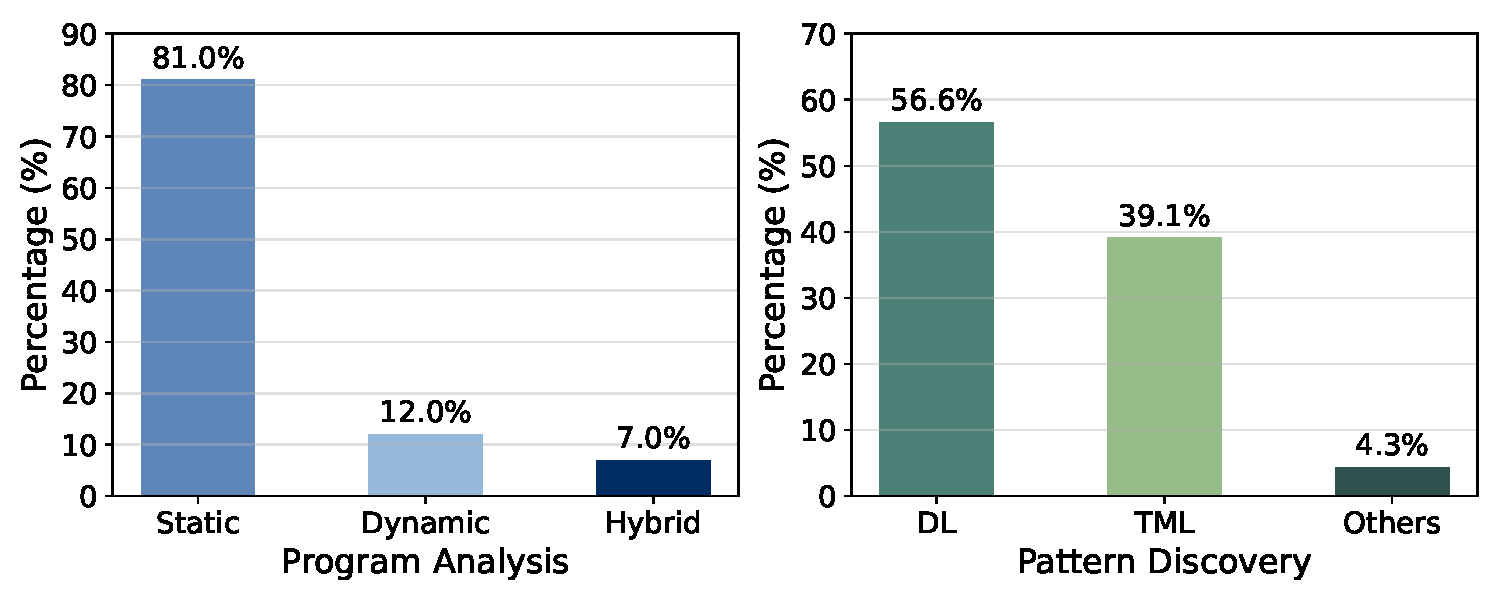
\includegraphics[width=0.76\linewidth]{fig/paper_tech.pdf}
    % \vspace{-0.1cm}
    \caption{The overall distribution of investigated approaches in Android malware detection.}
    \label{fig:paper_distribution}
    \vspace{-0.3cm}
\end{figure}

\bulletpoint{Systematic investigation}
To better understand the efforts dedicated to Android malware detection, we conduct a systematic literature review since 2011.
Aiming for the inclusion of a broad range of papers, we follow the search strategies used in~\cite{liu2022deep,liu2020review}.
Specifically, we perform searches in key digital libraries, such as the ACM Digital Library and IEEE Xplore, using specific keywords, including \texttt{android malware detection}, \texttt{android analysis}, and \texttt{android malware}.
Then, a careful screening of titles and introductions is followed to selectively exclude studies unrelated to our research topic.
This meticulous process ultimately leads to the identification of 258 related papers.

We subsequently categorize these papers based on the program analysis and pattern discovery techniques they employ.
Figure~\ref{fig:paper_distribution} shows the distribution of these techniques.
Our analysis reveals that \textit{static analysis} is the predominant technique utilized to extract features from apps, followed by \textit{dynamic} and \textit{hybrid analysis}.
For pattern discovery, \textit{machine learning}, including both traditional machine learning (TML) and deep learning (DL) models, are extensively used to identify malicious patterns.
Particularly notable is the significant increase in the utilization of static feature extraction and ML-based techniques in recent years. 
This evolving trend highlights the importance of our study, seeking to provide an in-depth understanding of the contemporary landscape in ML-based Android malware detection.

\DIFaddbegin \bulletpoint{Dataset considerations}
\DIFadd{Including mobile apps from multiple markets is essential for improving the representativeness of an Android malware dataset.
To incorporate diverse app sources, we select AndroZoo~\mbox{%DIFAUXCMD
\cite{allix2016androzoo} }\hskip0pt%DIFAUXCMD
as the primary data source, following common practice in prior studies~\mbox{%DIFAUXCMD
\cite{chen2023continuous,pendlebury2019tesseract}}\hskip0pt%DIFAUXCMD
. 
AndroZoo aggregates apps collected from multiple distribution channels, including Google Play as well as third-party markets such as Anzhi and AppChina, enabling the construction of a dataset that spans different app ecosystems rather than relying on a single market.
We acknowledge that, despite its scale and diversity, AndroZoo does not cover all existing Android markets.
In particular, some prominent regional app stores—such as Huawei AppGallery and other OEM-operated markets—are not included.
Incorporating apps from these additional sources could further enhance the comprehensiveness of the dataset, and we consider this an important direction for future work.
Nevertheless, during dataset construction, we explicitly ensured that our samples include applications originating from multiple markets within AndroZoo, including Google Play, VirusShare, AppChina, Anzhi, and VirusTotal, rather than being dominated by a single source.
Consequently, our analysis and findings are grounded in behaviors observed across diverse app markets, which mitigates the risk that our conclusions are driven by market-specific biases.
}

\DIFadd{Moreover, different app markets adopt security policies and vetting mechanisms, which can affect both the prevalence and behavioral characteristics of malware.
Although these vetting strategies often share common mechanisms --- such as signature-based scanning and heuristic analysis --- prior work has shown that they are inherently reactive and subject to non-negligible detection delays~\mbox{%DIFAUXCMD
\cite{grace2012riskranker,zhou2012dissecting}}\hskip0pt%DIFAUXCMD
.
To account for this, we intentionally adopt a long time span when constructing our dataset, allowing malicious apps to be labeled post hoc and increasing the likelihood that the collected malware samples are representative and behaviorally diverse.
While acknowledging the dataset's limitations, we believe that our primary dataset is sufficiently diverse and representative to support a meaningful and realistic evaluation of ML-based Android malware detectors.
}

\DIFadd{We assess the performance of the selected Android malware detectors using two datasets collected over different time periods: a primary dataset spanning 2010-2020 and an additional dataset from 2021-2024. The additional dataset is used to evaluate effectiveness, allowing us to examine whether detection performance trends remain consistent across temporally distinct Android ecosystems.
}

\DIFadd{For the effectiveness evaluation, we observe that detection trends are consistent across both datasets, with similar performance rankings among the evaluated approaches. For example, HinDroid, Kim et al., and HomDroid achieve top performance in both time periods. This consistency indicates that our key findings regarding detection effectiveness are robust and generalizable across different time periods.
We further examine performance variations across datasets from different time periods in Section~\ref{effectiveness} (}\textit{\DIFadd{Detector stability of different time period dataset}}\DIFadd{). The results show that the effectiveness of these detectors remains relatively stable across the two periods, with only minor fluctuations in performance metrics. This observation further supports the conclusion that our findings derived from the primary dataset are applicable to more recent Android ecosystems as well.
For the robustness evaluation, the results are conceptually insensitive to the specific time period of the dataset. In malware evolution experiments, the key requirement is that training samples precede testing samples temporally. For obfuscation and adversarial evaluations, robustness is assessed by applying controlled transformations to testing apps, which does not depend on the absolute collection years of the dataset.
For the efficiency evaluation, we measure performance using the primary dataset while explicitly accounting for temporal changes in app characteristics. The decade-long span of this dataset is sufficient to capture substantial changes in app complexity and scale, enabling a meaningful assessment of efficiency trends.
}

\DIFadd{Overall, by combining effectiveness evaluation across two time periods with conceptually grounded robustness and efficiency analyses, our evaluation provides valuable insights into the performance characteristics of ML-based Android malware detectors, supporting the generalizability of our findings.
}

\bulletpoint{App packing and its impact}
\DIFadd{To protect applications from reverse engineering and tampering, many developers employ app packing techniques that obfuscate the original code structure~\mbox{%DIFAUXCMD
\cite{dong2022did,duan2018things}}\hskip0pt%DIFAUXCMD
.
Such techniques can substantially degrade the effectiveness of static analysis-based malware detectors, as they hinder the extraction of meaningful features from packed apps.
In this study, to systematically examine the state of ML-based Android malware detection, we focus primarily on unpacked apps, which is consistent with the scope of most prior work~\mbox{%DIFAUXCMD
\cite{chen2023continuous,wu2021homdroid}}\hskip0pt%DIFAUXCMD
.
During dataset construction, we identify an app as packed if it employs any known packing tools (}\textit{\DIFadd{e.g.,}} \DIFadd{Qihoo 360) and exclude these apps to ensure reliable static feature extraction.
We acknowledge that packing techniques can increase static feature extraction failure rates, negatively impacting the performance of static analysis-based detectors.
To mitigate this limitation in practical deployments, future detectors may benefit from integrating static and dynamic analysis techniques, enabling more robust feature extraction in the presence of packing and obfuscation.
In this work, our objective is to evaluate and understand the performance characteristics of ML-based Android malware detectors under controlled and comparable conditions.
A systematic investigation of app packing techniques and their impact on malware detection effectiveness is an important and complementary direction, which we leave for future work.
}

\DIFaddend \bulletpoint{Potential of large language models in Android malware analysis}
Large Language Models (LLMs) have demonstrated remarkable capabilities in natural language processing, code understanding, and reasoning tasks.
Building upon the findings and insights from our study, we believe that LLMs hold substantial promise in the domain of Android malware analysis, particularly in the following areas:
(1) Feature space exploration: LLMs can assist in selecting and combining discriminative features to enhance the performance of malware detectors.
By analyzing the impact of different feature sets on app behavior description, LLMs can guide the construction of more effective and concise feature representations.
(2) Semantic understanding of malicious behavior: LLMs can mine high-level malicious semantics directly from code, improving the interpretability of detection systems and offering deeper insight into the behavioral mechanisms of malware.

For example, LLMs can \DIFdelbegin \DIFdel{be employed to analyze various }\DIFdelend \DIFaddbegin \DIFadd{analyze multiple }\DIFaddend features that describe the same malicious behavior, \DIFdelbegin \DIFdel{assess their respective impacts on detector }\DIFdelend \DIFaddbegin \DIFadd{evaluate their relative impact on detection }\DIFaddend performance, and identify the most \DIFdelbegin \DIFdel{effective }\DIFdelend \DIFaddbegin \DIFadd{informative }\DIFaddend feature combinations for comprehensive behavior \DIFdelbegin \DIFdel{representation.
Furthermore}\DIFdelend \DIFaddbegin \DIFadd{modeling.
Moreover}\DIFaddend , LLMs can summarize the semantics of \DIFdelbegin \DIFdel{a group }\DIFdelend \DIFaddbegin \DIFadd{groups }\DIFaddend of functions within an application to uncover specific \DIFaddbegin \DIFadd{malicious }\DIFaddend operations—such as sensitive information collection, data exfiltration, or command-and-control communication.
These semantic summaries can then be \DIFdelbegin \DIFdel{used to enhance the characterization and }\DIFdelend \DIFaddbegin \DIFadd{leveraged to enhance app characterization and improve the }\DIFaddend detection of potentially malicious behaviors.

\bulletpoint{Threats to validity}
\jh{There are two main threats to the validity of our study.}
First, our research mainly focuses on investigating general ML-based Android malware detectors.
That is, we do not include the methods designed to solve a particular challenge like malware evolution.
Specifically, there have been several attempts~\cite{narayanan2016adaptive,zhang2020enhancing,chen2023continuous,xu2019droidevolver} starting to mitigate the challenges we have identified.
For instance, the recent APIGraph~\cite{zhang2020enhancing} identifies semantically similar API calls to enhance detectors' robustness against malware evolution.
Integrating this strategy with popular detectors like Drebin and MamaDroid leads to 5\% - 10\% detection improvements over a one-year malware evolution.
Nevertheless, our findings still hold, as these improvements are insufficient compared to the reduction of around 30\% observed in our study.
It is our aspiration that this study can motivate more researchers to focus on these challenges and develop effective solutions to mitigate them.

Second, inconsistencies might exist between our evaluation and the reported ones due to different settings, such as datasets, metrics, and toolchains.
To mitigate experimental biases and provide a fair comparison, we design a general-purpose framework.
Specifically, we adopt standardized techniques across all tasks, including feature extraction and ML modeling.
We also incorporate many evaluation scenarios, such as training data sizes, malware evolution, and efficiency, to ensure a comprehensive measurement using our crafted dataset.
It is our hope that the framework can facilitate future work in ML-based Android malware detection.
\DIFaddbegin 

\DIFaddend % \vspace{-0.2cm}
\section{Conclusion}
\label{sec:conclusion}
This paper performs the most extensive systematic study of the ML-based Android malware detection literature with empirical and quantitative analysis.
We identify challenges (\textit{i.e.,} unfair comparisons, unrealistic evaluations, and unclear computtational costs) that hinder the systematization in this field.
In response, we design a general-purpose framework for developing ML-based detection approaches and evaluating their effectiveness, robustness, and efficiency.
By experimentally comparing 12 representative approaches, our study paints a holistic view of the state of ML-based Android malware detection and puts forth recommendations to guide future research.
For instance, we find existing detectors are still vulnerable to malware evolution and adversarial attacks and in future work, we should focus on incorporating more \textit{malware semantics} to design more practical detectors.
Committed to the research community's growth, all the artifacts (code, data, and logs) are available at \url{https://anonymous.4open.science/r/RkRyb2lk}.
% Committed to the research community's growth, all the artifacts (code, data, and logs) will be released upon acceptance.


\clearpage
% \balance
\bibliographystyle{ACM-Reference-Format}
%%% -*-BibTeX-*-
%%% Do NOT edit. File created by BibTeX with style
%%% ACM-Reference-Format-Journals [18-Jan-2012].

\DIFdelbegin %DIFDELCMD < \begin{thebibliography}{110}
%DIFDELCMD < %%%
\DIFdelend \DIFaddbegin \begin{thebibliography}{117}
\DIFaddend 

%%% ====================================================================
%%% NOTE TO THE USER: you can override these defaults by providing
%%% customized versions of any of these macros before the \bibliography
%%% command.  Each of them MUST provide its own final punctuation,
%%% except for \shownote{} and \showURL{}.  The latter two
%%% do not use final punctuation, in order to avoid confusing it with
%%% the Web address.
%%%
%%% To suppress output of a particular field, define its macro to expand
%%% to an empty string, or better, \unskip, like this:
%%%
%%% \newcommand{\showURL}[1]{\unskip}   % LaTeX syntax
%%%
%%% \def \showURL #1{\unskip}           % plain TeX syntax
%%%
%%% ====================================================================

\ifx \showCODEN    \undefined \def \showCODEN     #1{\unskip}     \fi
\ifx \showISBNx    \undefined \def \showISBNx     #1{\unskip}     \fi
\ifx \showISBNxiii \undefined \def \showISBNxiii  #1{\unskip}     \fi
\ifx \showISSN     \undefined \def \showISSN      #1{\unskip}     \fi
\ifx \showLCCN     \undefined \def \showLCCN      #1{\unskip}     \fi
\ifx \shownote     \undefined \def \shownote      #1{#1}          \fi
\ifx \showarticletitle \undefined \def \showarticletitle #1{#1}   \fi
\ifx \showURL      \undefined \def \showURL       {\relax}        \fi
% The following commands are used for tagged output and should be
% invisible to TeX
\providecommand\bibfield[2]{#2}
\providecommand\bibinfo[2]{#2}
\providecommand\natexlab[1]{#1}
\providecommand\showeprint[2][]{arXiv:#2}

\bibitem[and({[n.\,d.]})]%
        {androguard}
 \bibinfo{year}{[n.\,d.]}\natexlab{}.
\newblock \bibinfo{title}{{Androguard}}.
\newblock \bibinfo{howpublished}{\url{https://github.com/androguard/}}.
\newblock


\bibitem[ang({[n.\,d.]})]%
        {angr}
 \bibinfo{year}{[n.\,d.]}\natexlab{}.
\newblock \bibinfo{title}{{Angr}}.
\newblock \bibinfo{howpublished}{\url{https://angr.io/}}.
\newblock


\bibitem[apk({[n.\,d.]})]%
        {apkt}
 \bibinfo{year}{[n.\,d.]}\natexlab{}.
\newblock \bibinfo{title}{{APKTool}}.
\newblock \bibinfo{howpublished}{\url{https://ibotpeaches.github.io/Apktool/}}.
\newblock


\bibitem[bac({[n.\,d.]})]%
        {backsmali}
 \bibinfo{year}{[n.\,d.]}\natexlab{}.
\newblock \bibinfo{title}{{BackSmali}}.
\newblock \bibinfo{howpublished}{\url{https://github.com/JesusFreke/smali}}.
\newblock


\bibitem[app({[n.\,d.]})]%
        {appnumber}
 \bibinfo{year}{[n.\,d.]}\natexlab{}.
\newblock \bibinfo{title}{{How Many Apps In Google Play Store?}}
\newblock
  \bibinfo{howpublished}{\url{https://www.bankmycell.com/blog/number-of-google-play-store-apps}}.
\newblock


\DIFaddbegin \bibitem[ida({[n.\,d.]})]%DIF > 
        {ida_pro}
 \DIFadd{\bibinfo{year}{[n.\,d.]}}\natexlab{}\DIFadd{.
}\newblock \DIFadd{\bibinfo{title}{{IDA Pro}}.
}\newblock \DIFadd{\bibinfo{howpublished}{\url{https://hex-rays.com/ida-pro/}}.
}\newblock


\DIFaddend \bibitem[kun({[n.\,d.]})]%
        {kungfu}
 \bibinfo{year}{[n.\,d.]}\natexlab{}.
\newblock \bibinfo{title}{{Kharon project}}.
\newblock
  \bibinfo{howpublished}{\url{https://cidre.gitlabpages.inria.fr/malware/malware-website/dataset/malware_DroidKungFu1.html}}.
\newblock


\bibitem[lib({[n.\,d.]})]%
        {libradar}
 \bibinfo{year}{[n.\,d.]}\natexlab{}.
\newblock \bibinfo{title}{{LibRadar}}.
\newblock \bibinfo{howpublished}{\url{https://github.com/pkumza/LibRadar}}.
\newblock


\bibitem[pyt({[n.\,d.]})]%
        {pytorch}
 \bibinfo{year}{[n.\,d.]}\natexlab{}.
\newblock \bibinfo{title}{{PyTorch}}.
\newblock \bibinfo{howpublished}{\url{https://pytorch.org/}}.
\newblock


\DIFaddbegin \bibitem[vs({[n.\,d.]})]%DIF > 
        {vs}
 \DIFadd{\bibinfo{year}{[n.\,d.]}}\natexlab{}\DIFadd{.
}\newblock \DIFadd{\bibinfo{title}{{VirusShare}}.
}\newblock \DIFadd{\bibinfo{howpublished}{\url{https://virusshare.com/}}.
}\newblock


\DIFaddend \bibitem[vir({[n.\,d.]})]%
        {virustotal}
 \bibinfo{year}{[n.\,d.]}\natexlab{}.
\newblock \bibinfo{title}{{VirusTotal}}.
\newblock \bibinfo{howpublished}{\url{https://www.virustotal.com}}.
\newblock


\bibitem[Aafer et~al\mbox{.}(2013)]%
        {aafer2013droidapiminer}
\bibfield{author}{\bibinfo{person}{Yousra Aafer}, \bibinfo{person}{Wenliang
  Du}, {and} \bibinfo{person}{Heng Yin}.} \bibinfo{year}{2013}\natexlab{}.
\newblock \showarticletitle{Droidapiminer: Mining api-level features for robust
  malware detection in android}. In \bibinfo{booktitle}{\emph{International
  ICST Conference, SecureComm}}.
\newblock


\bibitem[Allix et~al\mbox{.}(2016)]%
        {allix2016androzoo}
\bibfield{author}{\bibinfo{person}{Kevin Allix},
  \bibinfo{person}{Tegawend{\'e}~F Bissyand{\'e}}, \bibinfo{person}{Jacques
  Klein}, {and} \bibinfo{person}{Yves Le~Traon}.}
  \bibinfo{year}{2016}\natexlab{}.
\newblock \showarticletitle{Androzoo: Collecting millions of android apps for
  the research community}. In \bibinfo{booktitle}{\emph{MSR}}.
\newblock


\bibitem[Amin et~al\mbox{.}(2022)]%
        {amin2022android}
\bibfield{author}{\bibinfo{person}{Muhammad Amin}, \bibinfo{person}{Babar
  Shah}, \bibinfo{person}{Aizaz Sharif}, \bibinfo{person}{Tamleek Ali},
  \bibinfo{person}{Ki-Il Kim}, {and} \bibinfo{person}{Sajid Anwar}.}
  \bibinfo{year}{2022}\natexlab{}.
\newblock \showarticletitle{Android malware detection through generative
  adversarial networks}.
\newblock \bibinfo{journal}{\emph{Emerging Telecommunications Technologies}}
  (\bibinfo{year}{2022}).
\newblock


\bibitem[Aonzo et~al\mbox{.}(2020)]%
        {aonzo2020obfuscapk}
\bibfield{author}{\bibinfo{person}{Simone Aonzo},
  \bibinfo{person}{Gabriel~Claudiu Georgiu}, \bibinfo{person}{Luca Verderame},
  {and} \bibinfo{person}{Alessio Merlo}.} \bibinfo{year}{2020}\natexlab{}.
\newblock \showarticletitle{Obfuscapk: An open-source black-box obfuscation
  tool for Android apps}.
\newblock \bibinfo{journal}{\emph{SoftwareX}} (\bibinfo{year}{2020}).
\newblock


\bibitem[Arp et~al\mbox{.}(2022)]%
        {arp2022and}
\bibfield{author}{\bibinfo{person}{Daniel Arp}, \bibinfo{person}{Erwin
  Quiring}, \bibinfo{person}{Feargus Pendlebury}, \bibinfo{person}{Alexander
  Warnecke}, \bibinfo{person}{Fabio Pierazzi}, \bibinfo{person}{Christian
  Wressnegger}, \bibinfo{person}{Lorenzo Cavallaro}, {and}
  \bibinfo{person}{Konrad Rieck}.} \bibinfo{year}{2022}\natexlab{}.
\newblock \showarticletitle{Dos and don'ts of machine learning in computer
  security}. In \bibinfo{booktitle}{\emph{Security}}.
\newblock


\bibitem[Arp et~al\mbox{.}(2014)]%
        {arp2014drebin}
\bibfield{author}{\bibinfo{person}{Daniel Arp}, \bibinfo{person}{Michael
  Spreitzenbarth}, \bibinfo{person}{Malte Hubner}, \bibinfo{person}{Hugo
  Gascon}, \bibinfo{person}{Konrad Rieck}, {and} \bibinfo{person}{CERT
  Siemens}.} \bibinfo{year}{2014}\natexlab{}.
\newblock \showarticletitle{Drebin: Effective and explainable detection of
  android malware in your pocket.}. In \bibinfo{booktitle}{\emph{NDSS}}.
\newblock


\bibitem[Athalye et~al\mbox{.}(2018)]%
        {athalye2018obfuscated}
\bibfield{author}{\bibinfo{person}{Anish Athalye}, \bibinfo{person}{Nicholas
  Carlini}, {and} \bibinfo{person}{David Wagner}.}
  \bibinfo{year}{2018}\natexlab{}.
\newblock \showarticletitle{Obfuscated gradients give a false sense of
  security: Circumventing defenses to adversarial examples}. In
  \bibinfo{booktitle}{\emph{ICML}}.
\newblock


\bibitem[Au et~al\mbox{.}(2012)]%
        {au2012pscout}
\bibfield{author}{\bibinfo{person}{Kathy Wain~Yee Au}, \bibinfo{person}{Yi~Fan
  Zhou}, \bibinfo{person}{Zhen Huang}, {and} \bibinfo{person}{David Lie}.}
  \bibinfo{year}{2012}\natexlab{}.
\newblock \showarticletitle{Pscout: analyzing the android permission
  specification}. In \bibinfo{booktitle}{\emph{CCS}}.
\newblock


\bibitem[Backes et~al\mbox{.}(2016)]%
        {backes2016demystifying}
\bibfield{author}{\bibinfo{person}{Michael Backes}, \bibinfo{person}{Sven
  Bugiel}, \bibinfo{person}{Erik Derr}, \bibinfo{person}{Patrick McDaniel},
  \bibinfo{person}{Damien Octeau}, {and} \bibinfo{person}{Sebastian
  Weisgerber}.} \bibinfo{year}{2016}\natexlab{}.
\newblock \showarticletitle{On demystifying the android application
  framework:$\{$Re-Visiting$\}$ android permission specification analysis}. In
  \bibinfo{booktitle}{\emph{Security}}.
\newblock


\bibitem[Barbero et~al\mbox{.}(2022)]%
        {barbero2022transcending}
\bibfield{author}{\bibinfo{person}{Federico Barbero}, \bibinfo{person}{Feargus
  Pendlebury}, \bibinfo{person}{Fabio Pierazzi}, {and} \bibinfo{person}{Lorenzo
  Cavallaro}.} \bibinfo{year}{2022}\natexlab{}.
\newblock \showarticletitle{Transcending transcend: Revisiting malware
  classification in the presence of concept drift}. In
  \bibinfo{booktitle}{\emph{SP}}.
\newblock


\bibitem[Bhagoji et~al\mbox{.}(2018)]%
        {bhagoji2018enhancing}
\bibfield{author}{\bibinfo{person}{Arjun~Nitin Bhagoji},
  \bibinfo{person}{Daniel Cullina}, \bibinfo{person}{Chawin Sitawarin}, {and}
  \bibinfo{person}{Prateek Mittal}.} \bibinfo{year}{2018}\natexlab{}.
\newblock \showarticletitle{Enhancing robustness of machine learning systems
  via data transformations}. In \bibinfo{booktitle}{\emph{2018 52nd Annual
  Conference on Information Sciences and Systems (CISS)}}. IEEE.
\newblock


\DIFdelbegin %DIFDELCMD < \bibitem[Cai(2020)]%%%
%DIF < 
        %DIFDELCMD < {%%%
\DIFdel{cai2020assessing}%DIFDELCMD < }
%DIFDELCMD < %%%
\DIFdel{\bibfield{author}{\bibinfo{person}{Haipeng Cai}.}
  \bibinfo{year}{2020}}%DIFDELCMD < \natexlab{}%%%
\DIFdel{.
}%DIFDELCMD < \newblock \showarticletitle{Assessing and improving malware detection
%DIFDELCMD <   sustainability through app evolution studies}%%%
\DIFdel{.
}%DIFDELCMD < \newblock %%%
\DIFdel{\bibinfo{journal}{\emph{TOSEM}} (\bibinfo{year}{2020}).
}%DIFDELCMD < \newblock
%DIFDELCMD < 

%DIFDELCMD < %%%
\DIFdelend \bibitem[Cai et~al\mbox{.}(2021)]%
        {cai2021learning}
\bibfield{author}{\bibinfo{person}{Minghui Cai}, \bibinfo{person}{Yuan Jiang},
  \bibinfo{person}{Cuiying Gao}, \bibinfo{person}{Heng Li}, {and}
  \bibinfo{person}{Wei Yuan}.} \bibinfo{year}{2021}\natexlab{}.
\newblock \showarticletitle{Learning features from enhanced function call
  graphs for Android malware detection}.
\newblock \bibinfo{journal}{\emph{Neurocomputing}} (\bibinfo{year}{2021}).
\newblock


\bibitem[Carlini and Wagner(2017)]%
        {carlini2017towards}
\bibfield{author}{\bibinfo{person}{Nicholas Carlini} {and}
  \bibinfo{person}{David Wagner}.} \bibinfo{year}{2017}\natexlab{}.
\newblock \showarticletitle{Towards evaluating the robustness of neural
  networks}. In \bibinfo{booktitle}{\emph{S\&P}}.
\newblock


\bibitem[Ceschin et~al\mbox{.}(2020)]%
        {ceschin2020machine}
\bibfield{author}{\bibinfo{person}{Fabr{\'\i}cio Ceschin},
  \bibinfo{person}{Marcus Botacin}, \bibinfo{person}{Albert Bifet},
  \bibinfo{person}{Bernhard Pfahringer}, \bibinfo{person}{Luiz~S Oliveira},
  \bibinfo{person}{Heitor~Murilo Gomes}, {and} \bibinfo{person}{Andr{\'e}
  Gr{\'e}gio}.} \bibinfo{year}{2020}\natexlab{}.
\newblock \showarticletitle{Machine learning (in) security: A stream of
  problems}.
\newblock \bibinfo{journal}{\emph{Digital Threats: Research and Practice}}
  (\bibinfo{year}{2020}).
\newblock


\bibitem[Chen et~al\mbox{.}(2020)]%
        {chen2020denas}
\bibfield{author}{\bibinfo{person}{Simin Chen}, \bibinfo{person}{Soroush
  Bateni}, \bibinfo{person}{Sampath Grandhi}, \bibinfo{person}{Xiaodi Li},
  \bibinfo{person}{Cong Liu}, {and} \bibinfo{person}{Wei Yang}.}
  \bibinfo{year}{2020}\natexlab{}.
\newblock \showarticletitle{DENAS: automated rule generation by knowledge
  extraction from neural networks}. In \bibinfo{booktitle}{\emph{ESEC/FSE}}.
\newblock


\bibitem[Chen et~al\mbox{.}(2019)]%
        {chen2019android}
\bibfield{author}{\bibinfo{person}{Xiao Chen}, \bibinfo{person}{Chaoran Li},
  \bibinfo{person}{Derui Wang}, \bibinfo{person}{Sheng Wen},
  \bibinfo{person}{Jun Zhang}, \bibinfo{person}{Surya Nepal},
  \bibinfo{person}{Yang Xiang}, {and} \bibinfo{person}{Kui Ren}.}
  \bibinfo{year}{2019}\natexlab{}.
\newblock \showarticletitle{Android HIV: A study of repackaging malware for
  evading machine-learning detection}.
\newblock \bibinfo{journal}{\emph{TIFS}} (\bibinfo{year}{2019}).
\newblock


\bibitem[Chen et~al\mbox{.}(2023)]%
        {chen2023continuous}
\bibfield{author}{\bibinfo{person}{Yizheng Chen}, \bibinfo{person}{Zhoujie
  Ding}, {and} \bibinfo{person}{David Wagner}.}
  \bibinfo{year}{2023}\natexlab{}.
\newblock \showarticletitle{Continuous Learning for Android Malware Detection}.
\newblock \bibinfo{journal}{\emph{arXiv preprint arXiv:2302.04332}}
  (\bibinfo{year}{2023}).
\newblock


\bibitem[Daoudi et~al\mbox{.}(2021)]%
        {daoudi2021dexray}
\bibfield{author}{\bibinfo{person}{Nadia Daoudi}, \bibinfo{person}{Jordan
  Samhi}, \bibinfo{person}{Abdoul~Kader Kabore}, \bibinfo{person}{Kevin Allix},
  \bibinfo{person}{Tegawend{\'e}~F Bissyand{\'e}}, {and}
  \bibinfo{person}{Jacques Klein}.} \bibinfo{year}{2021}\natexlab{}.
\newblock \showarticletitle{Dexray: a simple, yet effective deep learning
  approach to android malware detection based on image representation of
  bytecode}. In \bibinfo{booktitle}{\emph{DMLSD}}.
\newblock


\bibitem[Ding et~al\mbox{.}(2023)]%
        {ding2020android}
\bibfield{author}{\bibinfo{person}{Yuxin Ding}, \bibinfo{person}{Xiao Zhang},
  \bibinfo{person}{Jieke Hu}, {and} \bibinfo{person}{Wenting Xu}.}
  \bibinfo{year}{2023}\natexlab{}.
\newblock \showarticletitle{Android malware detection method based on bytecode
  image}.
\newblock \bibinfo{journal}{\emph{Journal of Ambient Intelligence and Humanized
  Computing}} (\bibinfo{year}{2023}).
\newblock


\DIFaddbegin \bibitem[Dong et~al\mbox{.}(2022)]%DIF > 
        {dong2022did}
\DIFadd{\bibfield{author}{\bibinfo{person}{Zikan Dong}, \bibinfo{person}{Hongxuan Liu},
  \bibinfo{person}{Liu Wang}, \bibinfo{person}{Xiapu Luo}, \bibinfo{person}{Yao
  Guo}, \bibinfo{person}{Guoai Xu}, \bibinfo{person}{Xusheng Xiao}, {and}
  \bibinfo{person}{Haoyu Wang}.} \bibinfo{year}{2022}}\natexlab{}\DIFadd{.
}\newblock \showarticletitle{What did you pack in my app? a systematic analysis
  of commercial Android packers}\DIFadd{. In \bibinfo{booktitle}{\emph{Proceedings of
  the 30th ACM Joint European Software Engineering Conference and Symposium on
  the Foundations of Software Engineering}}. \bibinfo{pages}{1430--1440}.
}\newblock


\bibitem[Duan et~al\mbox{.}(2018)]%DIF > 
        {duan2018things}
\DIFadd{\bibfield{author}{\bibinfo{person}{Yue Duan}, \bibinfo{person}{Mu Zhang},
  \bibinfo{person}{Abhishek~Vasist BHASKAR}, \bibinfo{person}{Heng Yin},
  \bibinfo{person}{Xiaorui Pan}, \bibinfo{person}{Tongxin Li},
  \bibinfo{person}{Xueqiang Wang}, {and} \bibinfo{person}{XiaoFeng Wang}.}
  \bibinfo{year}{2018}}\natexlab{}\DIFadd{.
}\newblock \showarticletitle{Things you may not know about android (un) packers:
  A systematic study based on whole-system emulation}\DIFadd{.
}\newblock  \DIFadd{(\bibinfo{year}{2018}).
}\newblock


\DIFaddend \bibitem[Enck et~al\mbox{.}(2009)]%
        {enck2009lightweight}
\bibfield{author}{\bibinfo{person}{William Enck}, \bibinfo{person}{Machigar
  Ongtang}, {and} \bibinfo{person}{Patrick McDaniel}.}
  \bibinfo{year}{2009}\natexlab{}.
\newblock \showarticletitle{On lightweight mobile phone application
  certification}. In \bibinfo{booktitle}{\emph{CCS}}.
\newblock


\bibitem[Fan et~al\mbox{.}(2021)]%
        {fan2021heterogeneous}
\bibfield{author}{\bibinfo{person}{Yujie Fan}, \bibinfo{person}{Mingxuan Ju},
  \bibinfo{person}{Shifu Hou}, \bibinfo{person}{Yanfang Ye},
  \bibinfo{person}{Wenqiang Wan}, \bibinfo{person}{Kui Wang},
  \bibinfo{person}{Yinming Mei}, {and} \bibinfo{person}{Qi Xiong}.}
  \bibinfo{year}{2021}\natexlab{}.
\newblock \showarticletitle{Heterogeneous temporal graph transformer: An
  intelligent system for evolving android malware detection}. In
  \bibinfo{booktitle}{\emph{KDD}}.
\newblock


\bibitem[Faruki et~al\mbox{.}(2014)]%
        {faruki2014android}
\bibfield{author}{\bibinfo{person}{Parvez Faruki}, \bibinfo{person}{Ammar
  Bharmal}, \bibinfo{person}{Vijay Laxmi}, \bibinfo{person}{Vijay Ganmoor},
  \bibinfo{person}{Manoj~Singh Gaur}, \bibinfo{person}{Mauro Conti}, {and}
  \bibinfo{person}{Muttukrishnan Rajarajan}.} \bibinfo{year}{2014}\natexlab{}.
\newblock \showarticletitle{Android security: a survey of issues, malware
  penetration, and defenses}.
\newblock \bibinfo{journal}{\emph{IEEE communications surveys tutorials}}
  (\bibinfo{year}{2014}).
\newblock


\bibitem[Feng et~al\mbox{.}(2019)]%
        {feng2019mobidroid}
\bibfield{author}{\bibinfo{person}{Ruitao Feng}, \bibinfo{person}{Sen Chen},
  \bibinfo{person}{Xiaofei Xie}, \bibinfo{person}{Lei Ma},
  \bibinfo{person}{Guozhu Meng}, \bibinfo{person}{Yang Liu}, {and}
  \bibinfo{person}{Shang-Wei Lin}.} \bibinfo{year}{2019}\natexlab{}.
\newblock \showarticletitle{Mobidroid: A performance-sensitive malware
  detection system on mobile platform}. In \bibinfo{booktitle}{\emph{ICECCS}}.
  IEEE.
\newblock


\bibitem[Feng et~al\mbox{.}(2020)]%
        {feng2020performance}
\bibfield{author}{\bibinfo{person}{Ruitao Feng}, \bibinfo{person}{Sen Chen},
  \bibinfo{person}{Xiaofei Xie}, \bibinfo{person}{Guozhu Meng},
  \bibinfo{person}{Shang-Wei Lin}, {and} \bibinfo{person}{Yang Liu}.}
  \bibinfo{year}{2020}\natexlab{}.
\newblock \showarticletitle{A performance-sensitive malware detection system
  using deep learning on mobile devices}.
\newblock \bibinfo{journal}{\emph{TIFS}} (\bibinfo{year}{2020}).
\newblock


\bibitem[Gao et~al\mbox{.}(2024)]%
        {gao2024comprehensive}
\bibfield{author}{\bibinfo{person}{Cuiying Gao}, \bibinfo{person}{Gaozhun
  Huang}, \bibinfo{person}{Heng Li}, \bibinfo{person}{Bang Wu},
  \bibinfo{person}{Yueming Wu}, {and} \bibinfo{person}{Wei Yuan}.}
  \bibinfo{year}{2024}\natexlab{}.
\newblock \showarticletitle{A Comprehensive Study of Learning-based Android
  Malware Detectors under Challenging Environments}. In
  \bibinfo{booktitle}{\emph{ICSE}}.
\newblock


\bibitem[Gao et~al\mbox{.}(2021)]%
        {gao2021gdroid}
\bibfield{author}{\bibinfo{person}{Han Gao}, \bibinfo{person}{Shaoyin Cheng},
  {and} \bibinfo{person}{Weiming Zhang}.} \bibinfo{year}{2021}\natexlab{}.
\newblock \showarticletitle{GDroid: Android malware detection and
  classification with graph convolutional network}.
\newblock \bibinfo{journal}{\emph{Computers \& Security}}
  (\bibinfo{year}{2021}).
\newblock


\bibitem[Garcia et~al\mbox{.}(2018)]%
        {garcia2018lightweight}
\bibfield{author}{\bibinfo{person}{Joshua Garcia}, \bibinfo{person}{Mahmoud
  Hammad}, {and} \bibinfo{person}{Sam Malek}.} \bibinfo{year}{2018}\natexlab{}.
\newblock \showarticletitle{Lightweight, obfuscation-resilient detection and
  family identification of android malware}.
\newblock \bibinfo{journal}{\emph{TOSEM}} (\bibinfo{year}{2018}).
\newblock


\bibitem[Girshick(2015)]%
        {girshick2015fast}
\bibfield{author}{\bibinfo{person}{Ross Girshick}.}
  \bibinfo{year}{2015}\natexlab{}.
\newblock \showarticletitle{Fast r-cnn}. In \bibinfo{booktitle}{\emph{ICCV}}.
\newblock


\bibitem[Goodfellow et~al\mbox{.}(2014)]%
        {goodfellow2014generative}
\bibfield{author}{\bibinfo{person}{Ian Goodfellow}, \bibinfo{person}{Jean
  Pouget-Abadie}, \bibinfo{person}{Mehdi Mirza}, \bibinfo{person}{Bing Xu},
  \bibinfo{person}{David Warde-Farley}, \bibinfo{person}{Sherjil Ozair},
  \bibinfo{person}{Aaron Courville}, {and} \bibinfo{person}{Yoshua Bengio}.}
  \bibinfo{year}{2014}\natexlab{}.
\newblock \showarticletitle{Generative adversarial nets}. In
  \bibinfo{booktitle}{\emph{NIPS}}.
\newblock


\DIFaddbegin \bibitem[Grace et~al\mbox{.}(2012)]%DIF > 
        {grace2012riskranker}
\DIFadd{\bibfield{author}{\bibinfo{person}{Michael Grace}, \bibinfo{person}{Yajin
  Zhou}, \bibinfo{person}{Qiang Zhang}, \bibinfo{person}{Shihong Zou}, {and}
  \bibinfo{person}{Xuxian Jiang}.} \bibinfo{year}{2012}}\natexlab{}\DIFadd{.
}\newblock \showarticletitle{Riskranker: scalable and accurate zero-day android
  malware detection}\DIFadd{. In \bibinfo{booktitle}{\emph{Proceedings of the 10th
  international conference on Mobile systems, applications, and services}}.
  \bibinfo{pages}{281--294}.
}\newblock


\DIFaddend \bibitem[Grosse et~al\mbox{.}(2017)]%
        {grosse2017adversarial}
\bibfield{author}{\bibinfo{person}{Kathrin Grosse}, \bibinfo{person}{Nicolas
  Papernot}, \bibinfo{person}{Praveen Manoharan}, \bibinfo{person}{Michael
  Backes}, {and} \bibinfo{person}{Patrick McDaniel}.}
  \bibinfo{year}{2017}\natexlab{}.
\newblock \showarticletitle{Adversarial examples for malware detection}. In
  \bibinfo{booktitle}{\emph{ESORICS}}.
\newblock


\bibitem[He et~al\mbox{.}(2017)]%
        {he2017mask}
\bibfield{author}{\bibinfo{person}{Kaiming He}, \bibinfo{person}{Georgia
  Gkioxari}, \bibinfo{person}{Piotr Doll{\'a}r}, {and} \bibinfo{person}{Ross
  Girshick}.} \bibinfo{year}{2017}\natexlab{}.
\newblock \showarticletitle{Mask r-cnn}. In \bibinfo{booktitle}{\emph{CVPR}}.
\newblock


\bibitem[He and Kim(2019)]%
        {he2019malware}
\bibfield{author}{\bibinfo{person}{Ke He} {and} \bibinfo{person}{Dong-Seong
  Kim}.} \bibinfo{year}{2019}\natexlab{}.
\newblock \showarticletitle{Malware detection with malware images using deep
  learning techniques}. In \bibinfo{booktitle}{\emph{TrustCom}}.
\newblock


\bibitem[He et~al\mbox{.}(2023)]%
        {he2023efficient}
\bibfield{author}{\bibinfo{person}{Ping He}, \bibinfo{person}{Yifan Xia},
  \bibinfo{person}{Xuhong Zhang}, {and} \bibinfo{person}{Shouling Ji}.}
  \bibinfo{year}{2023}\natexlab{}.
\newblock \showarticletitle{Efficient Query-Based Attack against ML-Based
  Android Malware Detection under Zero Knowledge Setting}. In
  \bibinfo{booktitle}{\emph{CCS}}.
\newblock


\bibitem[He et~al\mbox{.}(2022)]%
        {he2022msdroid}
\bibfield{author}{\bibinfo{person}{Yiling He}, \bibinfo{person}{Yiping Liu},
  \bibinfo{person}{Lei Wu}, \bibinfo{person}{Ziqi Yang}, \bibinfo{person}{Kui
  Ren}, {and} \bibinfo{person}{Zhan Qin}.} \bibinfo{year}{2022}\natexlab{}.
\newblock \showarticletitle{Msdroid: Identifying malicious snippets for android
  malware detection}.
\newblock \bibinfo{journal}{\emph{TDSC}} (\bibinfo{year}{2022}).
\newblock


\bibitem[Hinton(2009)]%
        {hinton2009deep}
\bibfield{author}{\bibinfo{person}{Geoffrey Hinton}.}
  \bibinfo{year}{2009}\natexlab{}.
\newblock \showarticletitle{Deep belief networks}.
\newblock \bibinfo{journal}{\emph{Scholarpedia}} (\bibinfo{year}{2009}).
\newblock


\bibitem[Hou et~al\mbox{.}(2017)]%
        {hou2017hindroid}
\bibfield{author}{\bibinfo{person}{Shifu Hou}, \bibinfo{person}{Yanfang Ye},
  \bibinfo{person}{Yangqiu Song}, {and} \bibinfo{person}{Melih Abdulhayoglu}.}
  \bibinfo{year}{2017}\natexlab{}.
\newblock \showarticletitle{Hindroid: An intelligent android malware detection
  system based on structured heterogeneous information network}. In
  \bibinfo{booktitle}{\emph{KDD}}.
\newblock


\bibitem[Hsien-De~Huang and Kao(2018)]%
        {hsien2018r2}
\bibfield{author}{\bibinfo{person}{TonTon Hsien-De~Huang} {and}
  \bibinfo{person}{Hung-Yu Kao}.} \bibinfo{year}{2018}\natexlab{}.
\newblock \showarticletitle{R2-d2: Color-inspired convolutional neural network
  (cnn)-based android malware detections}. In \bibinfo{booktitle}{\emph{Big
  Data}}. IEEE.
\newblock


\bibitem[Huang et~al\mbox{.}(2019)]%
        {huang2019deep}
\bibfield{author}{\bibinfo{person}{Na Huang}, \bibinfo{person}{Ming Xu},
  \bibinfo{person}{Ning Zheng}, \bibinfo{person}{Tong Qiao}, {and}
  \bibinfo{person}{Kim-Kwang~Raymond Choo}.} \bibinfo{year}{2019}\natexlab{}.
\newblock \showarticletitle{Deep android malware classification with API-based
  feature graph}. In \bibinfo{booktitle}{\emph{TrustCom/BigDataSE}}.
\newblock


\bibitem[Jordaney et~al\mbox{.}(2017)]%
        {jordaney2017transcend}
\bibfield{author}{\bibinfo{person}{Roberto Jordaney}, \bibinfo{person}{Kumar
  Sharad}, \bibinfo{person}{Santanu~K Dash}, \bibinfo{person}{Zhi Wang},
  \bibinfo{person}{Davide Papini}, \bibinfo{person}{Ilia Nouretdinov}, {and}
  \bibinfo{person}{Lorenzo Cavallaro}.} \bibinfo{year}{2017}\natexlab{}.
\newblock \showarticletitle{Transcend: Detecting concept drift in malware
  classification models}. In \bibinfo{booktitle}{\emph{Security}}.
\newblock


\bibitem[Karbab and Debbabi(2021)]%
        {karbab2021petadroid}
\bibfield{author}{\bibinfo{person}{ElMouatez~Billah Karbab} {and}
  \bibinfo{person}{Mourad Debbabi}.} \bibinfo{year}{2021}\natexlab{}.
\newblock \showarticletitle{Petadroid: adaptive android malware detection using
  deep learning}. In \bibinfo{booktitle}{\emph{DIMVA}}.
\newblock


\bibitem[Karbab et~al\mbox{.}(2018)]%
        {karbab2018maldozer}
\bibfield{author}{\bibinfo{person}{ElMouatez~Billah Karbab},
  \bibinfo{person}{Mourad Debbabi}, \bibinfo{person}{Abdelouahid Derhab}, {and}
  \bibinfo{person}{Djedjiga Mouheb}.} \bibinfo{year}{2018}\natexlab{}.
\newblock \showarticletitle{MalDozer: Automatic framework for android malware
  detection using deep learning}.
\newblock \bibinfo{journal}{\emph{Digital Investigation}}
  (\bibinfo{year}{2018}).
\newblock


\bibitem[Kim et~al\mbox{.}(2018)]%
        {kim2018multimodal}
\bibfield{author}{\bibinfo{person}{TaeGuen Kim}, \bibinfo{person}{BooJoong
  Kang}, \bibinfo{person}{Mina Rho}, \bibinfo{person}{Sakir Sezer}, {and}
  \bibinfo{person}{Eul~Gyu Im}.} \bibinfo{year}{2018}\natexlab{}.
\newblock \showarticletitle{A multimodal deep learning method for android
  malware detection using various features}.
\newblock \bibinfo{journal}{\emph{TIFS}} (\bibinfo{year}{2018}).
\newblock


\bibitem[Kipf and Welling(2016)]%
        {kipf2016semi}
\bibfield{author}{\bibinfo{person}{Thomas~N Kipf} {and} \bibinfo{person}{Max
  Welling}.} \bibinfo{year}{2016}\natexlab{}.
\newblock \showarticletitle{Semi-supervised classification with graph
  convolutional networks}.
\newblock \bibinfo{journal}{\emph{arXiv preprint arXiv:1609.02907}}
  (\bibinfo{year}{2016}).
\newblock


\DIFdelbegin %DIFDELCMD < \bibitem[Lei et~al\mbox{.}(2019)]%%%
\bibitem[Le and Mikolov(2014)]{le2014distributed}
\DIFdelbegin \DIFdel{\bibfield{author}{\bibinfo{person}{Tao Lei}, \bibinfo{person}{Zhan Qin},
  \bibinfo{person}{Zhibo Wang}, \bibinfo{person}{Qi Li}, {and}
  \bibinfo{person}{Dengpan Ye}.} \bibinfo{year}{2019}}\DIFdelend \DIFaddbegin \DIFadd{\bibfield{author}{\bibinfo{person}{Quoc Le} {and} \bibinfo{person}{Tomas
  Mikolov}.} \bibinfo{year}{2014}}\DIFaddend \natexlab{}.
\newblock \DIFdelbegin %DIFDELCMD < \showarticletitle{EveDroid: Event-aware Android malware detection
%DIFDELCMD <   against model degrading for IoT devices}%%%
\DIFdel{. }%DIFDELCMD < \newblock %%%
\DIFdel{\bibinfo{journal}{\emph{IoTJ}} (\bibinfo{year}{2019})}\DIFdelend \DIFaddbegin \showarticletitle{Distributed representations of sentences and
  documents}\DIFadd{. In \bibinfo{booktitle}{\emph{ICML}}}\DIFaddend .
\newblock


\bibitem[Li et~al\mbox{.}(2023)]%
        {li2023black}
\bibfield{author}{\bibinfo{person}{Heng Li}, \bibinfo{person}{Zhang Cheng},
  \bibinfo{person}{Bang Wu}, \bibinfo{person}{Liheng Yuan},
  \bibinfo{person}{Cuiying Gao}, \bibinfo{person}{Wei Yuan}, {and}
  \bibinfo{person}{Xiapu Luo}.} \bibinfo{year}{2023}\natexlab{}.
\newblock \showarticletitle{Black-box Adversarial Example Attack towards FCG
  Based Android Malware Detection under Incomplete Feature Information}. In
  \bibinfo{booktitle}{\emph{Security}}.
\newblock


\bibitem[Li et~al\mbox{.}(2019)]%
        {li2019adversarial}
\bibfield{author}{\bibinfo{person}{Heng Li}, \bibinfo{person}{ShiYao Zhou},
  \bibinfo{person}{Wei Yuan}, \bibinfo{person}{Jiahuan Li}, {and}
  \bibinfo{person}{Henry Leung}.} \bibinfo{year}{2019}\natexlab{}.
\newblock \showarticletitle{Adversarial-example attacks toward android malware
  detection system}.
\newblock \bibinfo{journal}{\emph{IEEE Systems Journal}}
  (\bibinfo{year}{2019}).
\newblock


\bibitem[Li et~al\mbox{.}(2021b)]%
        {li2021robust}
\bibfield{author}{\bibinfo{person}{Heng Li}, \bibinfo{person}{Shiyao Zhou},
  \bibinfo{person}{Wei Yuan}, \bibinfo{person}{Xiapu Luo},
  \bibinfo{person}{Cuiying Gao}, {and} \bibinfo{person}{Shuiyan Chen}.}
  \bibinfo{year}{2021}\natexlab{b}.
\newblock \showarticletitle{Robust android malware detection against
  adversarial example attacks}. In \bibinfo{booktitle}{\emph{WWW}}.
\newblock


\bibitem[Li et~al\mbox{.}(2021a)]%
        {li2021palmtree}
\bibfield{author}{\bibinfo{person}{Xuezixiang Li}, \bibinfo{person}{Yu Qu},
  {and} \bibinfo{person}{Heng Yin}.} \bibinfo{year}{2021}\natexlab{a}.
\newblock \showarticletitle{Palmtree: Learning an assembly language model for
  instruction embedding}. In \bibinfo{booktitle}{\emph{CCS}}.
\newblock


\bibitem[Liu et~al\mbox{.}(2020)]%
        {liu2020review}
\bibfield{author}{\bibinfo{person}{Kaijun Liu}, \bibinfo{person}{Shengwei Xu},
  \bibinfo{person}{Guoai Xu}, \bibinfo{person}{Miao Zhang},
  \bibinfo{person}{Dawei Sun}, {and} \bibinfo{person}{Haifeng Liu}.}
  \bibinfo{year}{2020}\natexlab{}.
\newblock \showarticletitle{A review of android malware detection approaches
  based on machine learning}.
\newblock \bibinfo{journal}{\emph{IEEE Access}} (\bibinfo{year}{2020}).
\newblock


\bibitem[Liu et~al\mbox{.}(2022)]%
        {liu2022deep}
\bibfield{author}{\bibinfo{person}{Yue Liu}, \bibinfo{person}{Chakkrit
  Tantithamthavorn}, \bibinfo{person}{Li Li}, {and} \bibinfo{person}{Yepang
  Liu}.} \bibinfo{year}{2022}\natexlab{}.
\newblock \showarticletitle{Deep learning for android malware defenses: a
  systematic literature review}.
\newblock \bibinfo{journal}{\emph{Comput. Surveys}} (\bibinfo{year}{2022}).
\newblock


\bibitem[Mariconti et~al\mbox{.}(2017)]%
        {mariconti2016mamadroid}
\bibfield{author}{\bibinfo{person}{Enrico Mariconti}, \bibinfo{person}{Lucky
  Onwuzurike}, \bibinfo{person}{Panagiotis Andriotis},
  \bibinfo{person}{Emiliano De~Cristofaro}, \bibinfo{person}{Gordon Ross},
  {and} \bibinfo{person}{Gianluca Stringhini}.}
  \bibinfo{year}{2017}\natexlab{}.
\newblock \showarticletitle{Mamadroid: Detecting android malware by building
  markov chains of behavioral models}. In \bibinfo{booktitle}{\emph{NDSS}}.
\newblock


\bibitem[Mart{\'\i}n et~al\mbox{.}(2017)]%
        {martin2017evolving}
\bibfield{author}{\bibinfo{person}{Alejandro Mart{\'\i}n},
  \bibinfo{person}{F{\'e}lix Fuentes-Hurtado}, \bibinfo{person}{Valery
  Naranjo}, {and} \bibinfo{person}{David Camacho}.}
  \bibinfo{year}{2017}\natexlab{}.
\newblock \showarticletitle{Evolving deep neural networks architectures for
  android malware classification}. In \bibinfo{booktitle}{\emph{2017 IEEE
  Congress on Evolutionary Computation (CEC)}}. IEEE.
\newblock


\bibitem[McLaughlin et~al\mbox{.}(2017)]%
        {mclaughlin2017deep}
\bibfield{author}{\bibinfo{person}{Niall McLaughlin}, \bibinfo{person}{Jesus
  Martinez~del Rincon}, \bibinfo{person}{BooJoong Kang},
  \bibinfo{person}{Suleiman Yerima}, \bibinfo{person}{Paul Miller},
  \bibinfo{person}{Sakir Sezer}, \bibinfo{person}{Yeganeh Safaei},
  \bibinfo{person}{Erik Trickel}, \bibinfo{person}{Ziming Zhao},
  \bibinfo{person}{Adam Doup{\'e}}, {et~al\mbox{.}}}
  \bibinfo{year}{2017}\natexlab{}.
\newblock \showarticletitle{Deep android malware detection}. In
  \bibinfo{booktitle}{\emph{CODASPY}}.
\newblock


\bibitem[Medsker and Jain(2001)]%
        {medsker2001recurrent}
\bibfield{author}{\bibinfo{person}{Larry~R Medsker} {and} \bibinfo{person}{LC
  Jain}.} \bibinfo{year}{2001}\natexlab{}.
\newblock \showarticletitle{Recurrent neural networks}.
\newblock \bibinfo{journal}{\emph{Design and Applications}}
  (\bibinfo{year}{2001}).
\newblock


\bibitem[Mikolov et~al\mbox{.}(2013)]%
        {mikolov2013distributed}
\bibfield{author}{\bibinfo{person}{Tomas Mikolov}, \bibinfo{person}{Ilya
  Sutskever}, \bibinfo{person}{Kai Chen}, \bibinfo{person}{Greg~S Corrado},
  {and} \bibinfo{person}{Jeff Dean}.} \bibinfo{year}{2013}\natexlab{}.
\newblock \showarticletitle{Distributed representations of words and phrases
  and their compositionality}. In \bibinfo{booktitle}{\emph{NIPS}}.
\newblock


\bibitem[Miller et~al\mbox{.}(2016)]%
        {miller2016reviewer}
\bibfield{author}{\bibinfo{person}{Brad Miller}, \bibinfo{person}{Alex
  Kantchelian}, \bibinfo{person}{Michael~Carl Tschantz}, \bibinfo{person}{Sadia
  Afroz}, \bibinfo{person}{Rekha Bachwani}, \bibinfo{person}{Riyaz
  Faizullabhoy}, \bibinfo{person}{Ling Huang}, \bibinfo{person}{Vaishaal
  Shankar}, \bibinfo{person}{Tony Wu}, \bibinfo{person}{George Yiu},
  {et~al\mbox{.}}} \bibinfo{year}{2016}\natexlab{}.
\newblock \showarticletitle{Reviewer integration and performance measurement
  for malware detection}. In \bibinfo{booktitle}{\emph{Detection of Intrusions
  and Malware, and Vulnerability Assessment: 13th International Conference,
  DIMVA 2016, San Sebasti{\'a}n, Spain, July 7-8, 2016}}.
\newblock


\bibitem[Narayanan et~al\mbox{.}(2017)]%
        {narayanan2017graph2vec}
\bibfield{author}{\bibinfo{person}{Annamalai Narayanan},
  \bibinfo{person}{Mahinthan Chandramohan}, \bibinfo{person}{Rajasekar
  Venkatesan}, \bibinfo{person}{Lihui Chen}, \bibinfo{person}{Yang Liu}, {and}
  \bibinfo{person}{Shantanu Jaiswal}.} \bibinfo{year}{2017}\natexlab{}.
\newblock \showarticletitle{graph2vec: Learning distributed representations of
  graphs}.
\newblock \bibinfo{journal}{\emph{arXiv:1707.05005}} (\bibinfo{year}{2017}).
\newblock


\bibitem[Narayanan et~al\mbox{.}(2016)]%
        {narayanan2016adaptive}
\bibfield{author}{\bibinfo{person}{Annamalai Narayanan}, \bibinfo{person}{Liu
  Yang}, \bibinfo{person}{Lihui Chen}, {and} \bibinfo{person}{Liu Jinliang}.}
  \bibinfo{year}{2016}\natexlab{}.
\newblock \showarticletitle{Adaptive and scalable android malware detection
  through online learning}. In \bibinfo{booktitle}{\emph{IJCNN}}. IEEE.
\newblock


\bibitem[Papernot et~al\mbox{.}(2016)]%
        {papernot2016distillation}
\bibfield{author}{\bibinfo{person}{Nicolas Papernot}, \bibinfo{person}{Patrick
  McDaniel}, \bibinfo{person}{Xi Wu}, \bibinfo{person}{Somesh Jha}, {and}
  \bibinfo{person}{Ananthram Swami}.} \bibinfo{year}{2016}\natexlab{}.
\newblock \showarticletitle{Distillation as a defense to adversarial
  perturbations against deep neural networks}. In
  \bibinfo{booktitle}{\emph{SP}}.
\newblock


\bibitem[Peiravian and Zhu(2013)]%
        {peiravian2013machine}
\bibfield{author}{\bibinfo{person}{Naser Peiravian} {and}
  \bibinfo{person}{Xingquan Zhu}.} \bibinfo{year}{2013}\natexlab{}.
\newblock \showarticletitle{Machine learning for android malware detection
  using permission and api calls}. In \bibinfo{booktitle}{\emph{2013 IEEE 25th
  international conference on tools with artificial intelligence}}. IEEE.
\newblock


\bibitem[Pekta{\c{s}} and Acarman(2020a)]%
        {pektacs2020deep}
\bibfield{author}{\bibinfo{person}{Abdurrahman Pekta{\c{s}}} {and}
  \bibinfo{person}{Tankut Acarman}.} \bibinfo{year}{2020}\natexlab{a}.
\newblock \showarticletitle{Deep learning for effective Android malware
  detection using API call graph embeddings}.
\newblock \bibinfo{journal}{\emph{Soft Computing}} (\bibinfo{year}{2020}).
\newblock


\bibitem[Pekta{\c{s}} and Acarman(2020b)]%
        {pektacs2020learning}
\bibfield{author}{\bibinfo{person}{Abdurrahman Pekta{\c{s}}} {and}
  \bibinfo{person}{Tankut Acarman}.} \bibinfo{year}{2020}\natexlab{b}.
\newblock \showarticletitle{Learning to detect Android malware via opcode
  sequences}.
\newblock \bibinfo{journal}{\emph{Neurocomputing}} (\bibinfo{year}{2020}).
\newblock


\bibitem[Pendlebury et~al\mbox{.}(2019)]%
        {pendlebury2019tesseract}
\bibfield{author}{\bibinfo{person}{Feargus Pendlebury}, \bibinfo{person}{Fabio
  Pierazzi}, \bibinfo{person}{Roberto Jordaney}, \bibinfo{person}{Johannes
  Kinder}, \bibinfo{person}{Lorenzo Cavallaro}, {et~al\mbox{.}}}
  \bibinfo{year}{2019}\natexlab{}.
\newblock \showarticletitle{TESSERACT: Eliminating experimental bias in malware
  classification across space and time}. In
  \bibinfo{booktitle}{\emph{Security}}.
\newblock


\bibitem[Pierazzi et~al\mbox{.}(2020)]%
        {pierazzi2020problemspace}
\bibfield{author}{\bibinfo{person}{Fabio Pierazzi}, \bibinfo{person}{Feargus
  Pendlebury}, \bibinfo{person}{Jacopo Cortellazzi}, {and}
  \bibinfo{person}{Lorenzo Cavallaro}.} \bibinfo{year}{2020}\natexlab{}.
\newblock \showarticletitle{Intriguing Properties of Adversarial ML Attacks in
  the Problem Space}. In \bibinfo{booktitle}{\emph{2020 IEEE Symposium on
  Security and Privacy (SP)}}. \bibinfo{publisher}{IEEE}.
\newblock


\bibitem[Qiu et~al\mbox{.}(2020)]%
        {qiu2020survey}
\bibfield{author}{\bibinfo{person}{Junyang Qiu}, \bibinfo{person}{Jun Zhang},
  \bibinfo{person}{Wei Luo}, \bibinfo{person}{Lei Pan}, \bibinfo{person}{Surya
  Nepal}, {and} \bibinfo{person}{Yang Xiang}.} \bibinfo{year}{2020}\natexlab{}.
\newblock \showarticletitle{A survey of android malware detection with deep
  neural models}.
\newblock \bibinfo{journal}{\emph{ACM Computing Surveys (CSUR)}}
  (\bibinfo{year}{2020}).
\newblock


\DIFaddbegin \bibitem[Souri and Hosseini(2018)]%DIF > 
        {souri2018state}
\DIFadd{\bibfield{author}{\bibinfo{person}{Alireza Souri} {and} \bibinfo{person}{Rahil
  Hosseini}.} \bibinfo{year}{2018}}\natexlab{}\DIFadd{.
}\newblock \showarticletitle{A state-of-the-art survey of malware detection
  approaches using data mining techniques}\DIFadd{.
}\newblock \DIFadd{\bibinfo{journal}{\emph{Human-centric Computing and Information
  Sciences}} \bibinfo{volume}{8}, \bibinfo{number}{1} (\bibinfo{year}{2018}),
  \bibinfo{pages}{1--22}.
}\newblock


\DIFaddend \bibitem[Su et~al\mbox{.}(2016)]%
        {su2016deep}
\bibfield{author}{\bibinfo{person}{Xin Su}, \bibinfo{person}{Dafang Zhang},
  \bibinfo{person}{Wenjia Li}, {and} \bibinfo{person}{Kai Zhao}.}
  \bibinfo{year}{2016}\natexlab{}.
\newblock \showarticletitle{A deep learning approach to android malware feature
  learning and detection}. In \bibinfo{booktitle}{\emph{Trustcom/BigDataSE}}.
\newblock


\bibitem[Sun et~al\mbox{.}(2019)]%
        {sun2019scalable}
\bibfield{author}{\bibinfo{person}{Bo Sun}, \bibinfo{person}{Tao Ban},
  \bibinfo{person}{Shun-Chieh Chang}, \bibinfo{person}{Yeali~S Sun},
  \bibinfo{person}{Takeshi Takahashi}, {and} \bibinfo{person}{Daisuke Inoue}.}
  \bibinfo{year}{2019}\natexlab{}.
\newblock \showarticletitle{A scalable and accurate feature representation
  method for identifying malicious mobile applications}. In
  \bibinfo{booktitle}{\emph{Proceedings of the 34th ACM/SIGAPP Symposium on
  Applied Computing}}.
\newblock


\bibitem[Sun et~al\mbox{.}(2017)]%
        {sun2017revisiting}
\bibfield{author}{\bibinfo{person}{Chen Sun}, \bibinfo{person}{Abhinav
  Shrivastava}, \bibinfo{person}{Saurabh Singh}, {and} \bibinfo{person}{Abhinav
  Gupta}.} \bibinfo{year}{2017}\natexlab{}.
\newblock \showarticletitle{Revisiting unreasonable effectiveness of data in
  deep learning era}. In \bibinfo{booktitle}{\emph{CVPR}}.
\newblock


\bibitem[Sun et~al\mbox{.}(2016a)]%
        {sun2016sigpid}
\bibfield{author}{\bibinfo{person}{Lichao Sun}, \bibinfo{person}{Zhiqiang Li},
  \bibinfo{person}{Qiben Yan}, \bibinfo{person}{Witawas Srisa-an}, {and}
  \bibinfo{person}{Yu Pan}.} \bibinfo{year}{2016}\natexlab{a}.
\newblock \showarticletitle{SigPID: significant permission identification for
  android malware detection}. In \bibinfo{booktitle}{\emph{2016 11th
  international conference on malicious and unwanted software (MALWARE)}}.
  IEEE.
\newblock


\bibitem[Sun et~al\mbox{.}(2016b)]%
        {sun2016taintart}
\bibfield{author}{\bibinfo{person}{Mingshen Sun}, \bibinfo{person}{Tao Wei},
  {and} \bibinfo{person}{John~CS Lui}.} \bibinfo{year}{2016}\natexlab{b}.
\newblock \showarticletitle{Taintart: A practical multi-level information-flow
  tracking system for android runtime}. In \bibinfo{booktitle}{\emph{CCS}}.
\newblock


\DIFaddbegin \bibitem[Sun et~al\mbox{.}(2011)]%DIF > 
        {sun2011pathsim}
\DIFadd{\bibfield{author}{\bibinfo{person}{Yizhou Sun}, \bibinfo{person}{Jiawei Han},
  \bibinfo{person}{Xifeng Yan}, \bibinfo{person}{Philip~S Yu}, {and}
  \bibinfo{person}{Tianyi Wu}.} \bibinfo{year}{2011}}\natexlab{}\DIFadd{.
}\newblock \showarticletitle{Pathsim: Meta path-based top-k similarity search in
  heterogeneous information networks}\DIFadd{.
}\newblock \DIFadd{\bibinfo{journal}{\emph{Proceedings of the VLDB Endowment}}
  (\bibinfo{year}{2011}).
}\newblock


\DIFaddend \bibitem[Sun et~al\mbox{.}(2010)]%
        {sun2010multiple}
\bibfield{author}{\bibinfo{person}{Zhaonan Sun}, \bibinfo{person}{Nawanol
  Ampornpunt}, \bibinfo{person}{Manik Varma}, {and} \bibinfo{person}{Svn
  Vishwanathan}.} \bibinfo{year}{2010}\natexlab{}.
\newblock \showarticletitle{Multiple kernel learning and the SMO algorithm}. In
  \bibinfo{booktitle}{\emph{NIPS}}.
\newblock


\bibitem[Suya et~al\mbox{.}(2020)]%
        {suya2020hybrid}
\bibfield{author}{\bibinfo{person}{Fnu Suya}, \bibinfo{person}{Jianfeng Chi},
  \bibinfo{person}{David Evans}, {and} \bibinfo{person}{Yuan Tian}.}
  \bibinfo{year}{2020}\natexlab{}.
\newblock \showarticletitle{Hybrid batch attacks: Finding black-box adversarial
  examples with limited queries}. In \bibinfo{booktitle}{\emph{Security}}.
\newblock


\bibitem[Vasilache et~al\mbox{.}(2018)]%
        {vasilache2018tensor}
\bibfield{author}{\bibinfo{person}{Nicolas Vasilache},
  \bibinfo{person}{Oleksandr Zinenko}, \bibinfo{person}{Theodoros Theodoridis},
  \bibinfo{person}{Priya Goyal}, \bibinfo{person}{Zachary DeVito},
  \bibinfo{person}{William~S Moses}, \bibinfo{person}{Sven Verdoolaege},
  \bibinfo{person}{Andrew Adams}, {and} \bibinfo{person}{Albert Cohen}.}
  \bibinfo{year}{2018}\natexlab{}.
\newblock \showarticletitle{Tensor comprehensions: Framework-agnostic
  high-performance machine learning abstractions}.
\newblock \bibinfo{journal}{\emph{arXiv preprint arXiv:1802.04730}}
  (\bibinfo{year}{2018}).
\newblock


\bibitem[Vinayakumar et~al\mbox{.}(2017)]%
        {vinayakumar2017deep}
\bibfield{author}{\bibinfo{person}{R Vinayakumar}, \bibinfo{person}{KP Soman},
  {and} \bibinfo{person}{Prabaharan Poornachandran}.}
  \bibinfo{year}{2017}\natexlab{}.
\newblock \showarticletitle{Deep android malware detection and classification}.
  In \bibinfo{booktitle}{\emph{2017 International conference on advances in
  computing, communications and informatics (ICACCI)}}. IEEE.
\newblock


\bibitem[Wang et~al\mbox{.}(2020)]%
        {wang2020sedroid}
\bibfield{author}{\bibinfo{person}{Ji Wang}, \bibinfo{person}{Qi Jing},
  \bibinfo{person}{Jianbo Gao}, {and} \bibinfo{person}{Xuanwei Qiu}.}
  \bibinfo{year}{2020}\natexlab{}.
\newblock \showarticletitle{SEdroid: A robust Android malware detector using
  selective ensemble learning}. In \bibinfo{booktitle}{\emph{2020 IEEE wireless
  communications and networking conference (WCNC)}}. IEEE.
\newblock


\bibitem[Wang et~al\mbox{.}(2019)]%
        {wang2019effective}
\bibfield{author}{\bibinfo{person}{Wei Wang}, \bibinfo{person}{Mengxue Zhao},
  {and} \bibinfo{person}{Jigang Wang}.} \bibinfo{year}{2019}\natexlab{}.
\newblock \showarticletitle{Effective android malware detection with a hybrid
  model based on deep autoencoder and convolutional neural network}.
\newblock \bibinfo{journal}{\emph{Journal of Ambient Intelligence and Humanized
  Computing}} (\bibinfo{year}{2019}).
\newblock


\bibitem[{Wikipedia contributors}({[n.\,d.]})]%
        {apkfile}
\bibfield{author}{\bibinfo{person}{{Wikipedia contributors}}.}
  \bibinfo{year}{[n.\,d.]}\natexlab{}.
\newblock \bibinfo{title}{{APK File Format}}.
\newblock
  \bibinfo{howpublished}{\url{https://en.wikipedia.org/wiki/Apk_file_format}}.
\newblock


\bibitem[Wu et~al\mbox{.}(2021a)]%
        {wu2021android}
\bibfield{author}{\bibinfo{person}{Bozhi Wu}, \bibinfo{person}{Sen Chen},
  \bibinfo{person}{Cuiyun Gao}, \bibinfo{person}{Lingling Fan},
  \bibinfo{person}{Yang Liu}, \bibinfo{person}{Weiping Wen}, {and}
  \bibinfo{person}{Michael~R Lyu}.} \bibinfo{year}{2021}\natexlab{a}.
\newblock \showarticletitle{Why an android app is classified as malware: Toward
  malware classification interpretation}.
\newblock \bibinfo{journal}{\emph{TOSEM}} (\bibinfo{year}{2021}).
\newblock


\bibitem[Wu et~al\mbox{.}(2016)]%
        {wu2016effective}
\bibfield{author}{\bibinfo{person}{Songyang Wu}, \bibinfo{person}{Pan Wang},
  \bibinfo{person}{Xun Li}, {and} \bibinfo{person}{Yong Zhang}.}
  \bibinfo{year}{2016}\natexlab{}.
\newblock \showarticletitle{Effective detection of android malware based on the
  usage of data flow APIs and machine learning}.
\newblock \bibinfo{journal}{\emph{Information and software technology}}
  (\bibinfo{year}{2016}).
\newblock


\bibitem[Wu et~al\mbox{.}(2019)]%
        {wu2019malscan}
\bibfield{author}{\bibinfo{person}{Yueming Wu}, \bibinfo{person}{Xiaodi Li},
  \bibinfo{person}{Deqing Zou}, \bibinfo{person}{Wei Yang},
  \bibinfo{person}{Xin Zhang}, {and} \bibinfo{person}{Hai Jin}.}
  \bibinfo{year}{2019}\natexlab{}.
\newblock \showarticletitle{Malscan: Fast market-wide mobile malware scanning
  by social-network centrality analysis}. In \bibinfo{booktitle}{\emph{ASE}}.
\newblock


\bibitem[Wu et~al\mbox{.}(2021b)]%
        {wu2021homdroid}
\bibfield{author}{\bibinfo{person}{Yueming Wu}, \bibinfo{person}{Deqing Zou},
  \bibinfo{person}{Wei Yang}, \bibinfo{person}{Xiang Li}, {and}
  \bibinfo{person}{Hai Jin}.} \bibinfo{year}{2021}\natexlab{b}.
\newblock \showarticletitle{HomDroid: detecting Android covert malware by
  social-network homophily analysis}. In \bibinfo{booktitle}{\emph{ISSTA}}.
\newblock


\bibitem[Xiao and Yang(2019)]%
        {xiao2019image}
\bibfield{author}{\bibinfo{person}{Xusheng Xiao} {and} \bibinfo{person}{Shao
  Yang}.} \bibinfo{year}{2019}\natexlab{}.
\newblock \showarticletitle{An image-inspired and cnn-based android malware
  detection approach}. In \bibinfo{booktitle}{\emph{ASE}}.
\newblock


\bibitem[Xu et~al\mbox{.}(2020)]%
        {xu2020sdac}
\bibfield{author}{\bibinfo{person}{Jiayun Xu}, \bibinfo{person}{Yingjiu Li},
  \bibinfo{person}{Robert~H Deng}, {and} \bibinfo{person}{Ke Xu}.}
  \bibinfo{year}{2020}\natexlab{}.
\newblock \showarticletitle{Sdac: A slow-aging solution for android malware
  detection using semantic distance based api clustering}.
\newblock \bibinfo{journal}{\emph{TDSC}} (\bibinfo{year}{2020}).
\newblock


\bibitem[Xu et~al\mbox{.}(2019)]%
        {xu2019droidevolver}
\bibfield{author}{\bibinfo{person}{Ke Xu}, \bibinfo{person}{Yingjiu Li},
  \bibinfo{person}{Robert Deng}, \bibinfo{person}{Kai Chen}, {and}
  \bibinfo{person}{Jiayun Xu}.} \bibinfo{year}{2019}\natexlab{}.
\newblock \showarticletitle{Droidevolver: Self-evolving android malware
  detection system}. In \bibinfo{booktitle}{\emph{EuroS\&P}}.
\newblock


\bibitem[Xu et~al\mbox{.}(2016)]%
        {xu2016iccdetector}
\bibfield{author}{\bibinfo{person}{Ke Xu}, \bibinfo{person}{Yingjiu Li}, {and}
  \bibinfo{person}{Robert~H Deng}.} \bibinfo{year}{2016}\natexlab{}.
\newblock \showarticletitle{Iccdetector: Icc-based malware detection on
  android}.
\newblock \bibinfo{journal}{\emph{TIFS}} (\bibinfo{year}{2016}).
\newblock


\bibitem[Xu et~al\mbox{.}(2018)]%
        {xu2018deeprefiner}
\bibfield{author}{\bibinfo{person}{Ke Xu}, \bibinfo{person}{Yingjiu Li},
  \bibinfo{person}{Robert~H Deng}, {and} \bibinfo{person}{Kai Chen}.}
  \bibinfo{year}{2018}\natexlab{}.
\newblock \showarticletitle{Deeprefiner: Multi-layer android malware detection
  system applying deep neural networks}. In
  \bibinfo{booktitle}{\emph{EuroS\&P}}.
\newblock


\bibitem[Yan et~al\mbox{.}(2018)]%
        {yan2018lstm}
\bibfield{author}{\bibinfo{person}{Jinpei Yan}, \bibinfo{person}{Yong Qi},
  {and} \bibinfo{person}{Qifan Rao}.} \bibinfo{year}{2018}\natexlab{}.
\newblock \showarticletitle{LSTM-based hierarchical denoising network for
  Android malware detection}.
\newblock \bibinfo{journal}{\emph{Security and Communication Networks}}
  (\bibinfo{year}{2018}).
\newblock


\bibitem[Yang et~al\mbox{.}(2021)]%
        {yang2021cade}
\bibfield{author}{\bibinfo{person}{Limin Yang}, \bibinfo{person}{Wenbo Guo},
  \bibinfo{person}{Qingying Hao}, \bibinfo{person}{Arridhana Ciptadi},
  \bibinfo{person}{Ali Ahmadzadeh}, \bibinfo{person}{Xinyu Xing}, {and}
  \bibinfo{person}{Gang Wang}.} \bibinfo{year}{2021}\natexlab{}.
\newblock \showarticletitle{$\{$CADE$\}$: Detecting and explaining concept
  drift samples for security applications}. In
  \bibinfo{booktitle}{\emph{Security}}.
\newblock


\bibitem[Ye et~al\mbox{.}(2019)]%
        {ye2019out}
\bibfield{author}{\bibinfo{person}{Yanfang Ye}, \bibinfo{person}{Shifu Hou},
  \bibinfo{person}{Lingwei Chen}, \bibinfo{person}{Jingwei Lei},
  \bibinfo{person}{Wenqiang Wan}, \bibinfo{person}{Jiabin Wang},
  \bibinfo{person}{Qi Xiong}, {and} \bibinfo{person}{Fudong Shao}.}
  \bibinfo{year}{2019}\natexlab{}.
\newblock \showarticletitle{Out-of-sample node representation learning for
  heterogeneous graph in real-time android malware detection}. In
  \bibinfo{booktitle}{\emph{IJCAI}}.
\newblock


\bibitem[Yuan et~al\mbox{.}(2014)]%
        {yuan2014droid}
\bibfield{author}{\bibinfo{person}{Zhenlong Yuan}, \bibinfo{person}{Yongqiang
  Lu}, \bibinfo{person}{Zhaoguo Wang}, {and} \bibinfo{person}{Yibo Xue}.}
  \bibinfo{year}{2014}\natexlab{}.
\newblock \showarticletitle{Droid-sec: deep learning in android malware
  detection}. In \bibinfo{booktitle}{\emph{SIGCOMM}}.
\newblock


\bibitem[Zegzhda et~al\mbox{.}(2018)]%
        {zegzhda2018applying}
\bibfield{author}{\bibinfo{person}{Peter Zegzhda}, \bibinfo{person}{Dmitry
  Zegzhda}, \bibinfo{person}{Evgeny Pavlenko}, {and} \bibinfo{person}{Gleb
  Ignatev}.} \bibinfo{year}{2018}\natexlab{}.
\newblock \showarticletitle{Applying deep learning techniques for Android
  malware detection}. In \bibinfo{booktitle}{\emph{Proceedings of the 11th
  International Conference on Security of Information and Networks}}.
\newblock


\bibitem[Zhang et~al\mbox{.}(2020)]%
        {zhang2020enhancing}
\bibfield{author}{\bibinfo{person}{Xiaohan Zhang}, \bibinfo{person}{Yuan
  Zhang}, \bibinfo{person}{Ming Zhong}, \bibinfo{person}{Daizong Ding},
  \bibinfo{person}{Yinzhi Cao}, \bibinfo{person}{Yukun Zhang},
  \bibinfo{person}{Mi Zhang}, {and} \bibinfo{person}{Min Yang}.}
  \bibinfo{year}{2020}\natexlab{}.
\newblock \showarticletitle{Enhancing state-of-the-art classifiers with api
  semantics to detect evolved android malware}. In
  \bibinfo{booktitle}{\emph{CCS}}.
\newblock


\bibitem[Zhao and Huang(2018)]%
        {zhao2018deepsim}
\bibfield{author}{\bibinfo{person}{Gang Zhao} {and} \bibinfo{person}{Jeff
  Huang}.} \bibinfo{year}{2018}\natexlab{}.
\newblock \showarticletitle{Deepsim: deep learning code functional similarity}.
  In \bibinfo{booktitle}{\emph{ESEC/FSE}}.
\newblock


\bibitem[Zhao et~al\mbox{.}(2021b)]%
        {zhao2021structural}
\bibfield{author}{\bibinfo{person}{Kaifa Zhao}, \bibinfo{person}{Hao Zhou},
  \bibinfo{person}{Yulin Zhu}, \bibinfo{person}{Xian Zhan},
  \bibinfo{person}{Kai Zhou}, \bibinfo{person}{Jianfeng Li},
  \bibinfo{person}{Le Yu}, \bibinfo{person}{Wei Yuan}, {and}
  \bibinfo{person}{Xiapu Luo}.} \bibinfo{year}{2021}\natexlab{b}.
\newblock \showarticletitle{Structural attack against graph based android
  malware detection}. In \bibinfo{booktitle}{\emph{CCS}}.
\newblock


\bibitem[Zhao et~al\mbox{.}(2021a)]%
        {zhao2021impact}
\bibfield{author}{\bibinfo{person}{Yanjie Zhao}, \bibinfo{person}{Li Li},
  \bibinfo{person}{Haoyu Wang}, \bibinfo{person}{Haipeng Cai},
  \bibinfo{person}{Tegawend{\'e}~F Bissyand{\'e}}, \bibinfo{person}{Jacques
  Klein}, {and} \bibinfo{person}{John Grundy}.}
  \bibinfo{year}{2021}\natexlab{a}.
\newblock \showarticletitle{On the impact of sample duplication in
  machine-learning-based android malware detection}.
\newblock \bibinfo{journal}{\emph{TOSEM}} (\bibinfo{year}{2021})\DIFaddbegin \DIFadd{.
}\newblock


\bibitem[Zhou and Jiang(2012)]%DIF > 
        {zhou2012dissecting}
\DIFadd{\bibfield{author}{\bibinfo{person}{Yajin Zhou} {and} \bibinfo{person}{Xuxian
  Jiang}.} \bibinfo{year}{2012}}\natexlab{}\DIFadd{.
}\newblock \showarticletitle{Dissecting android malware: Characterization and
  evolution}\DIFadd{. In \bibinfo{booktitle}{\emph{2012 IEEE symposium on security and
  privacy}}. IEEE, \bibinfo{pages}{95--109}}\DIFaddend .
\newblock


\bibitem[Zhou et~al\mbox{.}(2012)]%
        {zhou2012hey}
\bibfield{author}{\bibinfo{person}{Yajin Zhou}, \bibinfo{person}{Zhi Wang},
  \bibinfo{person}{Wu Zhou}, {and} \bibinfo{person}{Xuxian Jiang}.}
  \bibinfo{year}{2012}\natexlab{}.
\newblock \showarticletitle{Hey, you, get off of my market: detecting malicious
  apps in official and alternative android markets.}. In
  \bibinfo{booktitle}{\emph{NDSS}}.
\newblock


\bibitem[Zhu et~al\mbox{.}(2019a)]%
        {zhu2019fsnet}
\bibfield{author}{\bibinfo{person}{Dali Zhu}, \bibinfo{person}{Yuchen Ma},
  \bibinfo{person}{Tong Xi}, {and} \bibinfo{person}{Yiming Zhang}.}
  \bibinfo{year}{2019}\natexlab{a}.
\newblock \showarticletitle{FSNet: android malware detection with only one
  feature}. In \bibinfo{booktitle}{\emph{2019 IEEE Symposium on Computers and
  Communications (ISCC)}}. IEEE.
\newblock


\bibitem[Zhu et~al\mbox{.}(2019b)]%
        {zhu2019transparent}
\bibfield{author}{\bibinfo{person}{Dali Zhu}, \bibinfo{person}{Tong Xi},
  \bibinfo{person}{Pengfei Jing}, \bibinfo{person}{Di Wu},
  \bibinfo{person}{Qing Xia}, {and} \bibinfo{person}{Yiming Zhang}.}
  \bibinfo{year}{2019}\natexlab{b}.
\newblock \showarticletitle{A transparent and multimodal malware detection
  method for android apps}. In \bibinfo{booktitle}{\emph{Proceedings of the
  22nd international ACM conference on modeling, analysis and simulation of
  wireless and mobile systems}}.
\newblock


\bibitem[Zhu et~al\mbox{.}(2018)]%
        {zhu2018hemd}
\bibfield{author}{\bibinfo{person}{Hui-Juan Zhu}, \bibinfo{person}{Tong-Hai
  Jiang}, \bibinfo{person}{Bo Ma}, \bibinfo{person}{Zhu-Hong You},
  \bibinfo{person}{Wei-Lei Shi}, {and} \bibinfo{person}{Li Cheng}.}
  \bibinfo{year}{2018}\natexlab{}.
\newblock \showarticletitle{HEMD: a highly efficient random forest-based
  malware detection framework for Android}.
\newblock \bibinfo{journal}{\emph{Neural Computing and Applications}}
  (\bibinfo{year}{2018}).
\newblock


\bibitem[Zhu et~al\mbox{.}(2021)]%
        {zhu2021hybrid}
\bibfield{author}{\bibinfo{person}{Hui-Juan Zhu}, \bibinfo{person}{Liang-Min
  Wang}, \bibinfo{person}{Sheng Zhong}, \bibinfo{person}{Yang Li}, {and}
  \bibinfo{person}{Victor~S Sheng}.} \bibinfo{year}{2021}\natexlab{}.
\newblock \showarticletitle{A hybrid deep network framework for android malware
  detection}.
\newblock \bibinfo{journal}{\emph{IEEE Transactions on Knowledge and Data
  Engineering}} (\bibinfo{year}{2021}).
\newblock


\end{thebibliography}

\clearpage
\appendix
\section{Appendix}
This section contains additional data and information that can be of interest to the readers but that are not strictly necessary for understanding the main text.

% \subsection{Publication Statistics Overview}
% \label{sub:publication_statistics}

% We conduct a thorough review of literature spanning from 2011 to 2023 to explore prevalent techniques (\textit{i.e.,} program analysis and patten discovery) in Android malware detection.
% Here, program analysis refers to the methods used to extract features from APK files, while pattern discovery involves the strategies employed to discern patterns from these features.

% To capture as many relevant studies as possible, we take search strategies used in~\cite{liu2022deep,liu2020review}. 
% Our literature search spanned major digital libraries, such as the ACM Digital Library and IEEE Xplore. 
% Throughout the search process, we mainly employ specific keywords to pinpoint relevant papers, including \texttt{android malware detection}, \texttt{android analysis}, and \texttt{android malware}.
% A further manual review of titles and abstracts allows us to filter out papers unrelated to our topic.
% Ultimately, this process yields 258 related papers.

% \begin{figure}[h]
%     \centering
%     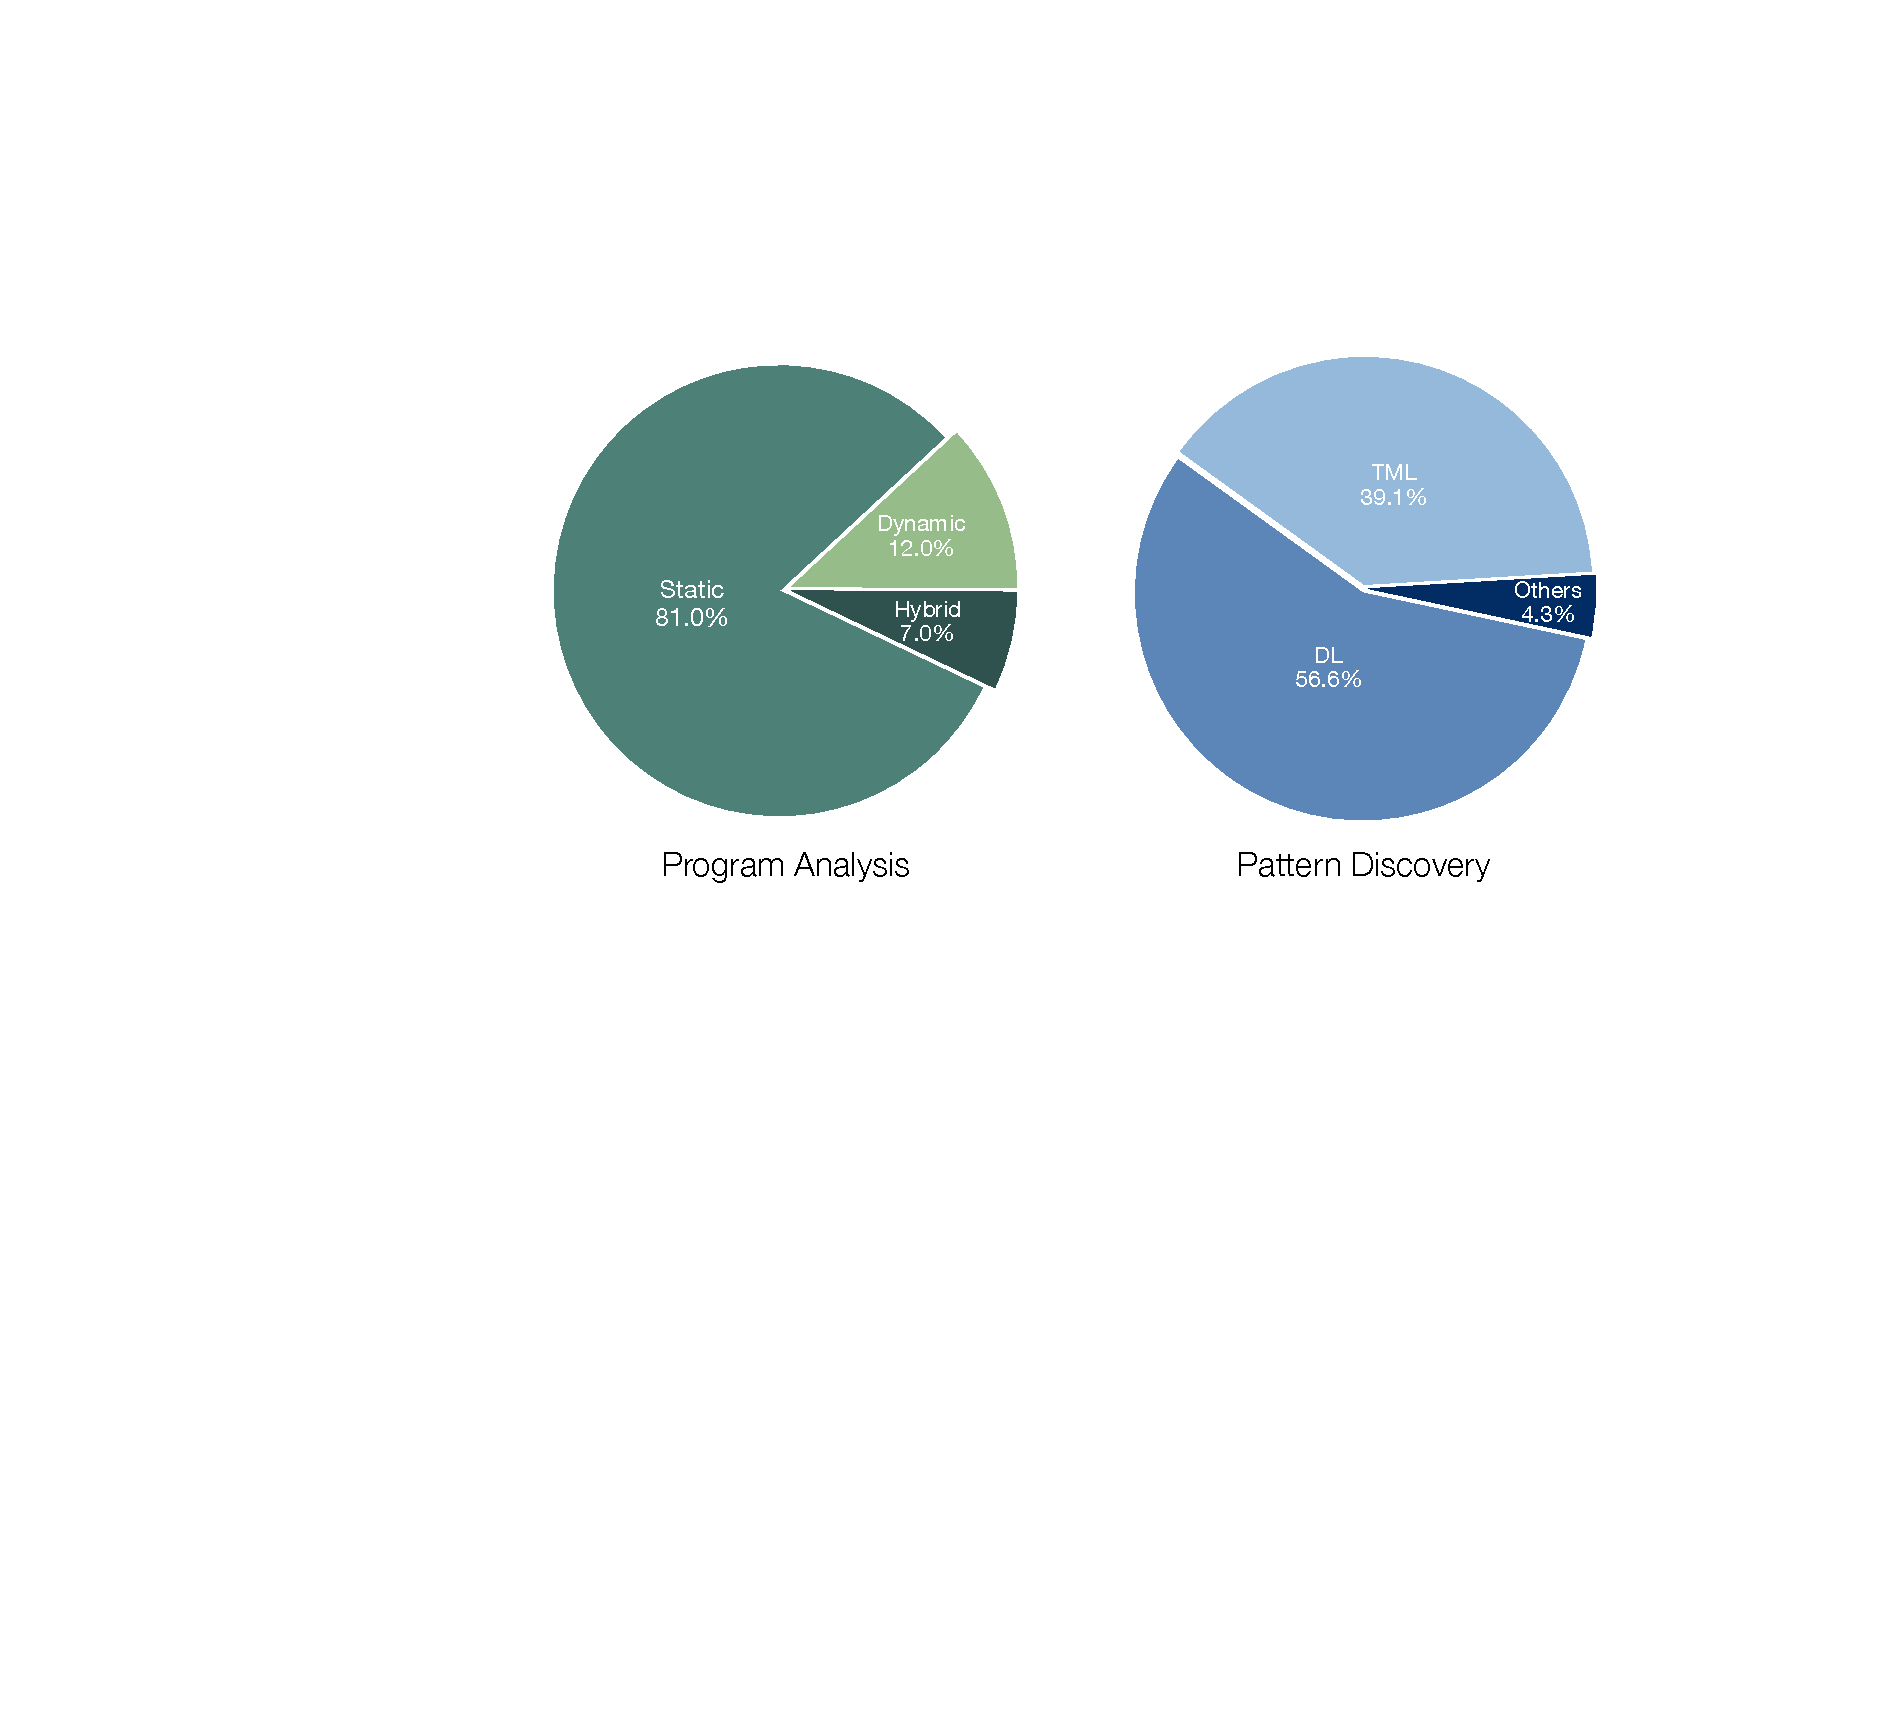
\includegraphics[width=0.73\linewidth]{fig/paper_distribution.pdf}
%     \caption{The overall distribution of investigated approaches from 2011 to 2023.}
%     \label{fig:paper_distribution}
%     \vspace{-0.3cm}
% \end{figure}


% We then categorize these papers based on the program analysis and pattern discovery techniques they employ.
% This distribution of these techniques is illustrated in Figure~\ref{fig:paper_distribution}.
% We observe that \textit{static analysis} emerges as the most favored program analysis technique, followed by \textit{dynamic analysis} and \textit{hybrid analysis}.
% Concurrently, \textit{machine learning (including both traditional machine learning and deep learning)} has been widely used to identify malware patterns.
% This observation further motivates us to focus on ML-based Android malware detection techniques that use static analysis.

\subsection{Feature Database}
\label{sub:feature_db}
To streamline the evaluation of different approaches, we establish a feature database to maintain commonly used features in Android malware detection.
Below, we outline the main features incorporated into the database, categorizing them for ease of reference.
\begin{itemize}[leftmargin=10pt]
    \setlength\itemsep{-1pt}
    \item \textit{Manifest}: this category contains features sourced from the \textit{AndroidManifest.xml} file, such as hardware components, permissions, intents, and app components.
    \item \textit{DisassembledCode}: this category includes the disassembled data extracted from the DEX file, such as the opcode, operands, and code strings.
    \item \textit{ProgramGraph}: this is mainly used to store the program graph of the APK file, including the nodes and edges.
    \item \textit{SharedLibrary}: this category contains the information of the shared libraries used by the APK file.
    \item \textit{Others}: this category includes other features that are not covered by the above categories.
\end{itemize}
Given the structure of the feature database, adding new features becomes straightforward, facilitating the adaptive evaluation of diverse approaches.
For instance, we can easily implement an add-on feature extractor and store the derived features in the database, waiting for use by the preprocessor.

% \vspace{-0.2cm}
% \subsection{\codename Implementation}
% \label{sub:implementation}
% \codename is developed in 17K lines of Python code.
% To ensure consistency and mitigate biases from different feature extraction toolchains and learning frameworks, we adopt standardized techniques across all tasks.
% For feature extraction, we use Androguard~\cite{androguard} to disassemble APK files and derive features such as permissions, intents, and program graphs. 
% LibRadar~\cite{libradar} helps in identifying third-party libraries within the applications, while Angr~\cite{angr} is used for analyzing native libraries and capturing essential features like opcodes and API calls. 
% When it comes to ML models, the scikit-learn library is our choice for traditional ML algorithms like SVM, KNN, and RF.
% On the other hand, for DL architectures such as CNN, GNN, and AE, we resort to Pytorch~\cite{pytorch}.
% This uniform approach ensures a balanced evaluation, concentrating purely on the uniqueness and performance of each method.

% \subsection{\codename Implementation}
% \label{sub:implementation}
% \codename is developed in 17K lines of Python code.
% To ensure consistency and mitigate biases from different feature extraction toolchains and learning frameworks, we adopt standardized techniques across all tasks.
% For feature extraction, we use Androguard~\cite{androguard} to disassemble APK files and derive features such as permissions, intents, and program graphs. 
% LibRadar~\cite{libradar} helps in identifying third-party libraries within the applications, while Angr~\cite{angr} is used for analyzing native libraries and capturing essential features like opcodes and API calls. 
% When it comes to ML models, the scikit-learn library is our choice for traditional ML algorithms like SVM, KNN, and RF.
% On the other hand, for DL architectures such as CNN, GNN, and AE, we resort to Pytorch~\cite{pytorch}.
% This uniform approach ensures a balanced evaluation, concentrating purely on the uniqueness and performance of each method.

\begin{table*}[t]
    \centering
    \caption{
    An overview of the 12 representative approaches we selected from major venues in security, software engineering, and machine learning. 
    \ymark \ indicates that the APK file (\textit{e.g.}, \textit{AndroidManifest.xml} for Manifest) is taken as input in Android malware detection, while \nmark \ is the opposite.
    \cmark \ and \xmark \ indicate whether feature engineering is handcrafted using domain knowledge or learned using representation learning.
    The effectiveness is based on the results reported in the original papers.}
    \vspace{-0.1cm}
    \begin{adjustbox}{width=\linewidth}
    \begin{tabular}{@{}c|cc|cccc|cc|rr|rrr@{}}
    \toprule
    \multirow{2}{*}{\raisebox{-0.3cm}{\textbf{\begin{tabular}[c]{@{}c@{}}Selected \\ Approach\end{tabular}}}} & \multicolumn{2}{c|}{\textbf{Publication}} & \multicolumn{4}{c|}{\textbf{Input from APK}} & \multicolumn{2}{c|}{\textbf{Feature Engineering}} & \multicolumn{2}{c|}{\textbf{Dataset}} & \multicolumn{3}{c}{\textbf{Effectiveness}} \\ \cmidrule(lr){2-3} \cmidrule(lr){4-7} \cmidrule(lr){8-9} \cmidrule(lr){10-11} \cmidrule(l){12-14}
     & \textbf{Venue} & \textbf{Year} & \textbf{Manifest} & \textbf{Dex} & \textbf{Resource} & \textbf{Library} & \textbf{Handcrafted} & \textbf{Learned} & \textbf{Malware} & \textbf{Goodware} & \textbf{TPR} & \textbf{FPR} & \textbf{F1} \\ \midrule
    Drebin\cite{arp2014drebin} & NDSS & 2014 & \ymark & \ymark & \nmark & \nmark & \cmark & \xmark & 5,560 & 123,453 & 94\% & \textbf{1\%} & 87\% \\ \midrule
    % ICCDetector\cite{xu2016iccdetector} & TIFS & 2016 & \ymark & \ymark & \nmark & \nmark & & & 5,264 & 12,026 & 93\% & \textbf{1\%} & 96\% \\ \midrule
    MamaDroid\cite{mariconti2016mamadroid} & NDSS & 2017 & \nmark & \ymark & \nmark & \nmark & \cmark & \xmark & 35,493 & 8,447 & 97\% & 2\% & 96\% \\ \midrule
    Mclaughlin et al.\cite{mclaughlin2017deep} & CODASPY & 2017 & \nmark & \ymark & \nmark & \nmark & \xmark& \cmark & 13,637 & 13,758 & 95\% & \textbf{1\%} & 97\% \\ \midrule
    HinDroid\cite{hou2017hindroid} & KDD & 2017 & \nmark & \ymark & \nmark & \nmark & \cmark & \xmark & 1,216 & 1,118 & \textbf{99\%} & 2\% & \textbf{99\%} \\ \midrule
    DeepRefiner\cite{xu2018deeprefiner} & EuroS\&P & 2018 & \ymark & \ymark & \ymark & \nmark & \xmark & \cmark & 62,915 & 47,525 & 98\% & 2\% & 98\% \\ \midrule
    Kim et al.\cite{kim2018multimodal} & TIFS & 2018 & \ymark & \ymark & \nmark & \ymark & \cmark & \cmark & 21,260 & 20,000 & \textbf{99\%} & \textbf{1\%} & \textbf{99\%} \\ \midrule
    MalScan\cite{wu2019malscan} & ASE & 2019 & \nmark & \ymark & \nmark & \nmark & \cmark & \xmark & 15,430 & 15,285 & --- & --- & 98\% \\ \midrule
    SDAC\cite{xu2020sdac} & TDSC & 2020 & \nmark & \ymark & \nmark & \nmark & \cmark & \cmark & 34,497 & 35,645 & 98\% & \textbf{1\%} & \textbf{99\%}\\ \midrule
    HomDroid\cite{wu2021homdroid} & ISSTA & 2021 & \nmark & \ymark & \nmark & \nmark & \cmark & \xmark & 3,358 & 4,840 & 97\% & 4\% & 95\% \\ \midrule
    Xmal\cite{wu2021android} & TOSEM & 2021 & \ymark & \ymark & \nmark & \nmark & \cmark & \xmark & 15,570 & 20,120 & 98\% & 2\% & 98\% \\ \midrule
    RAMDA\cite{li2021robust} & WWW & 2021 & \ymark & \ymark & \nmark & \nmark & \cmark & \xmark & 21,621 & 36,862 & 93\% & \textbf{1\%} & 90\% \\ \midrule
    MSDroid\cite{he2022msdroid} & TDSC & 2022 & \nmark & \ymark & \nmark & \nmark & \cmark & \xmark & 30,210 & 51,580 & 97\% & \textbf{1\%} & 97\% \\ \bottomrule
    \end{tabular}
    \end{adjustbox}
    \centering
    \begin{tablenotes}
    \footnotesize
    \item \ \ TPR, FPR, and F1 refer to true positive rate, false positive rate, and F1-score. 
    As MalScan is only evaluated on F1, its TPR and FPR are not available.
    \end{tablenotes}
    \label{tab:literature}
    \vspace{-0.3cm}
\end{table*}

\subsection{Reproduction of Selected Approaches}
\label{sub:approach_overview}
Table~\ref{tab:literature} offers a summary of the 12 representative approaches we have selected from leading publications in security~\cite{arp2014drebin,mariconti2016mamadroid,mclaughlin2017deep,xu2018deeprefiner,kim2018multimodal,xu2020sdac,he2022msdroid}, software engineering~\cite{wu2019malscan,wu2021homdroid,wu2021android}, and machine learning~\cite{hou2017hindroid,li2021robust}.
Within this table, we outline the publication details, input from APK, feature engineering style, dataset statistics, and their original effectiveness.
% As highlighted in Section~\ref{sec:discussion}, inconsistencies might exist between our quantitative evaluation results and those previously reported due to various biases, such as datasets, feature extraction toolchains, and learning frameworks.
To better support subsequent research and foster replicability and comparison, we provide the hyper-parameters of these approaches.

\bulletpoint{Drebin}
We replicate Drebin~\cite{arp2014drebin} utilizing a linear SVM with $C=1$, and set max number of iterations to $1000$.

\bulletpoint{MamaDroid}
MamaDroid~\cite{mariconti2016mamadroid} has two abstract mode \textit{i.e.}, package and family.
In our experiments, we choose the family mode, as it is more efficient in terms of time and memory.
For the RF classifier, we employ the default hyper-parameters provided by scikit-learn.

\bulletpoint{Mclaughlin et al}
Mclaughlin et al.~\cite{mclaughlin2017deep} is implemented with a CNN with one single convolutional layer, followed by a max-pooling layer and a fully connected layer.
The convolutional layer is configured with $32$ filters and a kernel size of $225*7$.
The fully connected layer has $16$ neurons.
For the evaluation process, a learning rate of $0.01$ and a batch size of $32$ are employed.
Additionally, inputs that exceed a length of $600000$ are truncated to $60000$, and those that are less than $600000$ are padded with zeros.

\bulletpoint{HinDroid}
In implementing HinDroid~\cite{hou2017hindroid}, various meta-path combinations have been tested. 
$AA^{T}$ yields remarkable performance in our experiments, and hence, is chosen as the meta-path.
For multi-kernel learning, we utilize the $p-norm$ multi-kernel learning framework as released by~\cite{sun2010multiple}, applying the default settings for the hyper-parameters.

\bulletpoint{DeepRefiner}
As discussed in Section~\ref{sub:selected_approaches}, DeepRefiner~\cite{xu2018deeprefiner} has two detection layers, and the second layer shows strong detection capability.
In our experiments, we replicate the second LSTM-based detection layer.
The model configuration is as follows: an embedding size of $16$ for word embeddings (bytecode instructions), a two-layer LSTM model with an input size of $16$, and a hidden size of $64$.
Batch size is set as $32$, and the learning rate is $0.001$.
The input sequence has a maximum length of $50,000$.
Inputs exceeding this length are truncated, while shorter inputs are padded with zeros.

\bulletpoint{Kim et al}
Kim et al.~\cite{kim2018multimodal} initially use a $5$ separated MLPs to process features from five various modalities, each with the same configuration.
Subsequently, a new MLP is introduced to integrate the learned features from the previous MLPs.
The initial five MLPs have layer configurations of $5000, 2500$, and $1000$ neurons.
The last MLP is structured with layers containing $1000, 500, 100$, and $10$ neurons, respectively.
A learning rate of $0.001$ and a batch size of $32$ are used during the training process.

\bulletpoint{MalScan}
The algorithm~\cite{wu2019malscan} is replicated with a KNN classifier, with the number of neighbors set to $3$.

\bulletpoint{SDAC}
SDAC~\cite{xu2020sdac} initially employs Word2Vec to encode API calls into vectors. Following this, K-means clustering is applied, and then these cluster centers are used as anchors to encode features.
In the classification phase, for simplicity, we use a linear SVM instead of multi-voting SVMs.
Additionally, due to K-means's randomness, the algorithm is executed $5$ times, and the average results are computed.
The size of Word2Vec embedding is set as $10$.
The chosen number of clusters is $1000$, and the SVM is configured using default parameters, allowing for $5000$ iterations.

\bulletpoint{HomDroid}
The approach~\cite{wu2021homdroid} is executed using a KNN classifier, with the number of neighbors set to $1$.

\bulletpoint{Xmal}
Xmal~\cite{wu2021android} is implemented using a 3-layer MLP with a hidden size of $64$.
An attention layer is also incorporated, utilizing an MLP with a hidden size of $158$.
The learning rate is set as $0.001$, and the batch size is $20$.

\bulletpoint{RAMDA}
RAMDA~\cite{li2021robust}'s architecture consists of two parts: autoencoder and classifier.
The encoder and decoder each consist of a 3-layer MLP with a hidden size of $600$.
The classifier is a 4-layer MLP with a hidden size of $600$.
During the training process, the autoencoder is trained first, and then the classifier is trained.
Configuration parameters are established with a learning rate of $0.001$, a batch size of $64$, and epochs set at $20$.
A pre-defined reconstruction loss of $30$ is used.
To constrain the loss, the positive weights are defined as $\lambda_1 = 10, \lambda_2 = 1, \lambda_3 = 10$.

\bulletpoint{MSDroid}
MSDroid~\cite{he2022msdroid} is implemented using a 3-layer GNN with a hidden size of $512$.
Subsequent to this, a 2-layer fully connected network with a hidden size of $512$ is used to classify the APKs.
The model's training parameters are set with a learning rate of $0.01$ and a batch size of $64$.

% \begin{figure}[t]
%     \centering
%     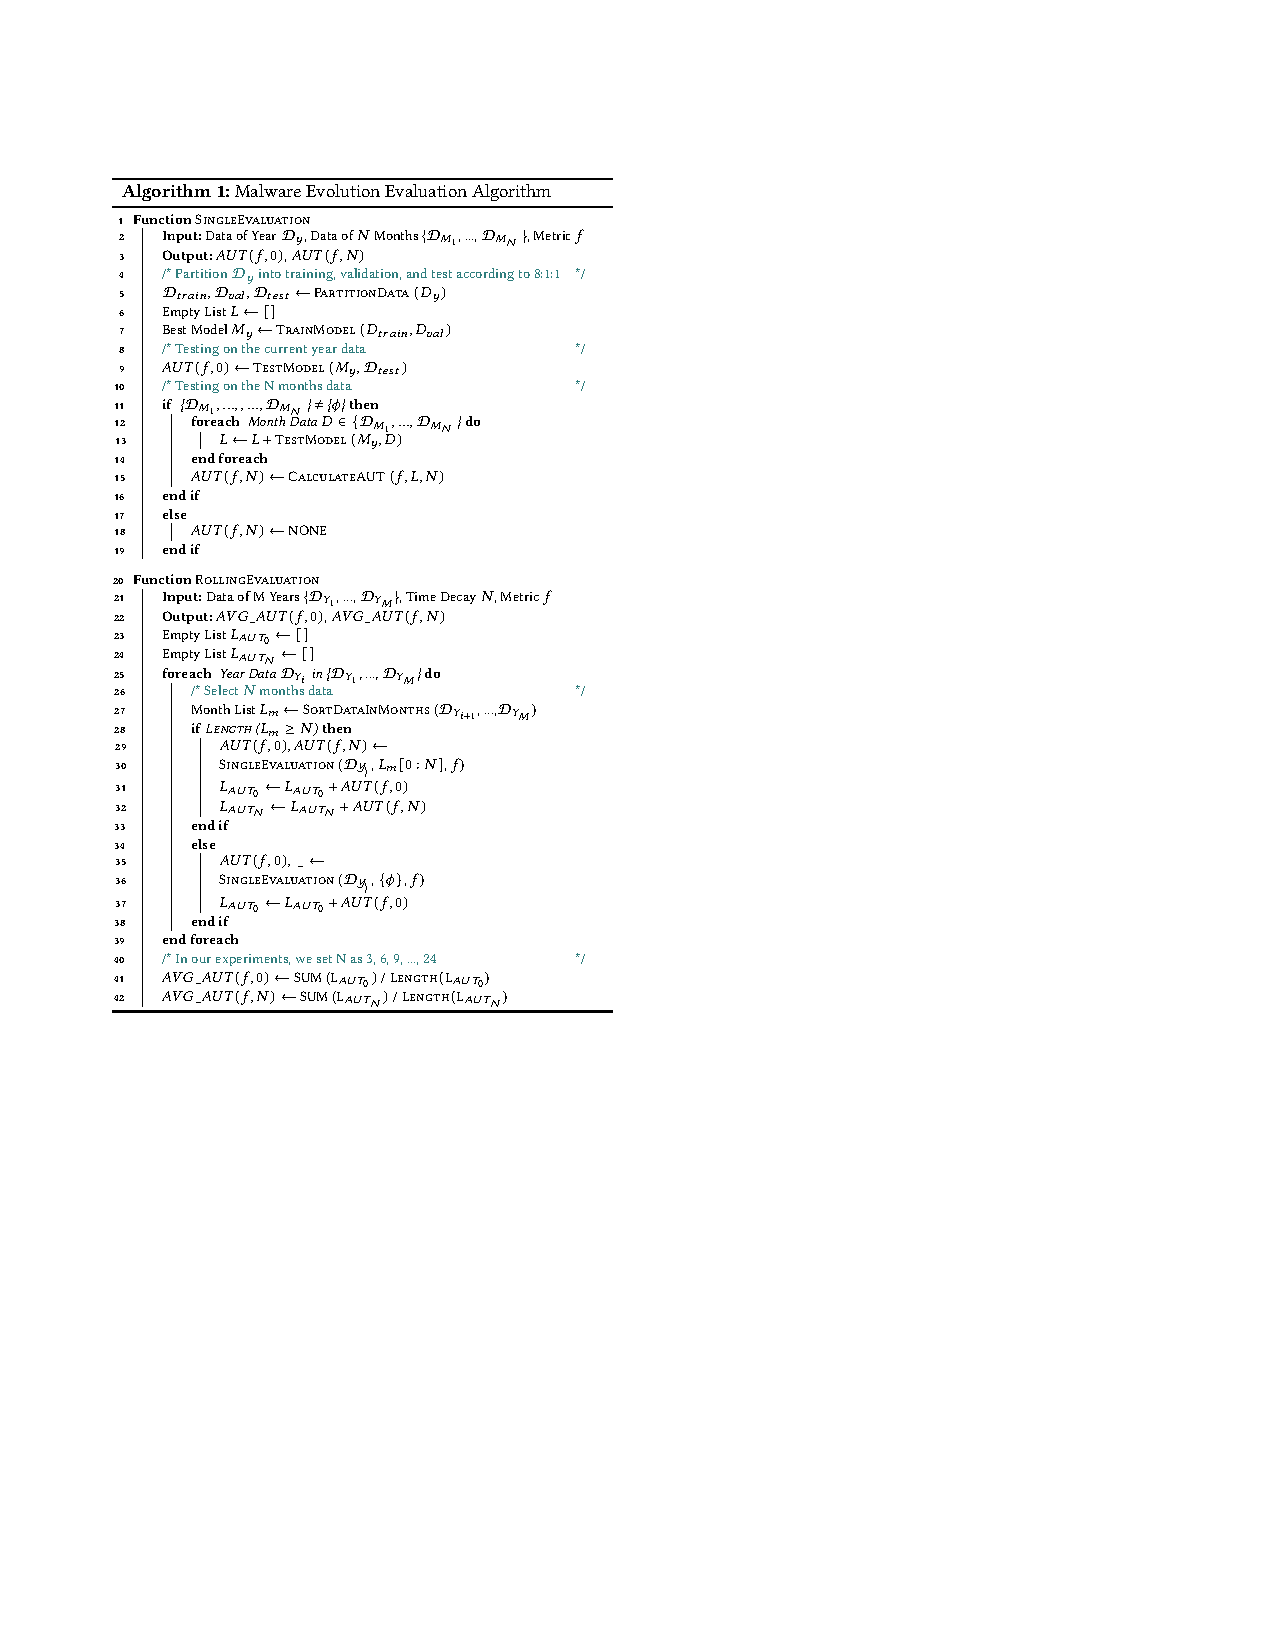
\includegraphics[width=0.86\linewidth]{fig/algorithm.pdf}
%     % \vspace{-0.3cm}
%     \caption{The rolling algorithm for evaluating the Android malware evolution.}
%     \label{fig:evolution_algorithm}
%     \vspace{-0.5cm}
% \end{figure}



\begin{table*}[t]
    \centering
    \renewcommand{\arraystretch}{1.1}
    \caption{The AUT(TPR, N) and AUT(FRP, N) of the selected approaches over varying time decays. In this analysis, we examine the shifts during various malware evolution periods: 3, 6, 9, 12, 15, 18, 21, and 24 months.}
    \vspace{-0.1cm}
    \begin{adjustbox}{width=\textwidth}
        \begin{tabular}{@{}c|c|c|c|c|c|c|c|c|c@{}}
            \toprule
            \textbf{Approach}         & \textbf{AUT(TPR,0)} & \textbf{AUT(TPR,3)} & \textbf{AUT(TPR,6)} & \textbf{AUT(TPR,9)} & \textbf{AUT(TPR,12)} & \textbf{AUT(TPR,15)} & \textbf{AUT(TPR,18)} & \textbf{AUT(TPR,21)} & \textbf{AUT(TPR,24)} \\ \midrule
            Drebin            & 0.803               & 0.722(-10.1\%)      & 0.670(-16.5\%)      & 0.601(-25.1\%)      & 0.564(-29.8\%)       & 0.530(-34.0\%)       & 0.508(-36.7\%)       & 0.484(-39.7\%)       & 0.466(-41.9\%)       \\ \midrule
            MamaDroid         & 0.712               & 0.496(-30.3\%)      & 0.429(-39.7\%)      & 0.365(-48.7\%)      & 0.322(-54.7\%)       & 0.308(-56.7\%)       & 0.282(-60.4\%)       & 0.253(-64.5\%)       & 0.233(-67.2\%)       \\ \midrule
            Mclaughlin et al. & 0.724               & 0.583(-19.6\%)      & 0.526(-27.3\%)      & 0.461(-36.4\%)      & 0.410(-43.4\%)       & 0.378(-47.9\%)       & 0.354(-51.2\%)       & 0.327(-54.9\%)       & 0.303(-58.1\%)       \\ \midrule
            HinDroid          & 0.831               & 0.786(-5.5\%)       & 0.773(-7.0\%)       & 0.729(-12.3\%)      & 0.687(-17.4\%)       & 0.684(-17.8\%)       & 0.674(-19.0\%)       & 0.662(-20.3\%)       & 0.655(-21.2\%)       \\ \midrule
            DeepRefiner       & 0.774               & 0.590(-23.7\%)      & 0.545(-29.6\%)      & 0.478(-38.3\%)      & 0.427(-44.8\%)       & 0.413(-46.6\%)       & 0.388(-49.9\%)       & 0.362(-53.2\%)       & 0.339(-56.2\%)       \\ \midrule
            Kim et al.        & 0.845               & 0.760(-10.0\%)      & 0.745(-11.8\%)      & 0.676(-20.0\%)      & 0.619(-26.7\%)       & 0.583(-31.0\%)       & 0.557(-34.0\%)       & 0.524(-38.0\%)       & 0.49(-42.0\%)        \\ \midrule
            MalScan           & 0.800               & 0.685(-14.4\%)      & 0.650(-18.8\%)      & 0.584(-27.0\%)      & 0.547(-31.6\%)       & 0.519(-35.2\%)       & 0.494(-38.3\%)       & 0.465(-41.8\%)       & 0.439(-45.1\%)       \\ \midrule
            SDAC              & 0.734               & 0.616(-16.1\%)      & 0.554(-24.5\%)      & 0.495(-32.6\%)      & 0.455(-38.0\%)       & 0.439(-40.2\%)       & 0.416(-43.4\%)       & 0.391(-46.8\%)       & 0.369(-49.7\%)       \\ \midrule
            HomDroid          & 0.836               & 0.689(-17.5\%)      & 0.651(-22.1\%)      & 0.596(-28.7\%)      & 0.546(-34.6\%)       & 0.515(-38.4\%)       & 0.486(-41.8\%)       & 0.448(-46.4\%)       & 0.422(-49.5\%)       \\ \midrule
            Xmal              & 0.836               & 0.741(-11.3\%)      & 0.693(-17.1\%)      & 0.617(-26.1\%)      & 0.575(-31.2\%)       & 0.550(-34.2\%)       & 0.523(-37.4\%)       & 0.492(-41.2\%)       & 0.463(-44.6\%)       \\ \midrule
            RAMDA             & 0.876               & 0.814(-7.0\%)       & 0.775(-11.6\%)      & 0.733(-16.3\%)      & 0.689(-21.3\%)       & 0.673(-23.2\%)       & 0.658(-24.8\%)       & 0.637(-27.2\%)       & 0.613(-30.1\%)       \\ \midrule
            MSDroid           & 0.835               & 0.755(-9.6\%)       & 0.732(-12.3\%)      & 0.673(-19.4\%)      & 0.635(-24.0\%)       & 0.632(-24.3\%)       & 0.604(-27.6\%)       & 0.569(-31.9\%)       & 0.544(-34.8\%)       \\ \midrule \midrule

            \textbf{Approach}         & \textbf{AUT(FPR,0)} & \textbf{AUT(FPR,3)} & \textbf{AUT(FPR,6)} & \textbf{AUT(FPR,9)} & \textbf{AUT(FPR,12)} & \textbf{AUT(FPR,15)} & \textbf{AUT(FPR,18)} & \textbf{AUT(FPR,21)} & \textbf{AUT(FPR,24)} \\ \midrule
            Drebin            & 0.014               & 0.02(+42.2\%)       & 0.023(+68.2\%)      & 0.024(+71.1\%)      & 0.026(+85.6\%)       & 0.029(+110.1\%)      & 0.030(+115.2\%)      & 0.031(+126.7\%)      & 0.033(+141.2\%)      \\ \midrule
            MamaDroid         & 0.009               & 0.010(+17.9\%)      & 0.011(+28.4\%)      & 0.010(+20.2\%)      & 0.011(+31.9\%)       & 0.013(+50.5\%)       & 0.013(+54.0\%)       & 0.014(+62.2\%)       & 0.014(+59.9\%)       \\ \midrule
            Mclaughlin et al. & 0.013               & 0.010(-19.1\%)      & 0.012(-7.5\%)       & 0.013(+1.9\%)       & 0.015(+14.3\%)       & 0.016(+23.6\%)       & 0.016(+24.4\%)       & 0.016(+22.1\%)       & 0.016(+20.5\%)       \\ \midrule
            HinDroid          & 0.016               & 0.262(+1491.6\%)    & 0.266(+1516.6\%)    & 0.271(+1548.8\%)    & 0.279(+1599.3\%)     & 0.319(+1839.1\%)     & 0.321(+1853.7\%)     & 0.324(+1873.8\%)     & 0.327(+1890.3\%)     \\ \midrule
            DeepRefiner       & 0.017               & 0.019(+9.3\%)       & 0.018(+5.9\%)       & 0.019(+7.6\%)       & 0.021(+20.3\%)       & 0.022(+27.2\%)       & 0.022(+28.9\%)       & 0.023(+31.2\%)       & 0.024(+38.7\%)       \\ \midrule
            Kim et al.        & 0.014               & 0.017(+19.7\%)      & 0.018(+29.8\%)      & 0.018(+31.9\%)      & 0.02(+43.5\%)        & 0.024(+75.9\%)       & 0.026(+84.6\%)       & 0.027(+91.8\%)       & 0.027(+95.4\%)       \\ \midrule
            MalScan           & 0.025               & 0.029(+17.1\%)      & 0.029(+18.7\%)      & 0.029(+17.9\%)      & 0.031(+24.8\%)       & 0.031(+26.1\%)       & 0.033(+33.0\%)       & 0.035(+40.7\%)       & 0.037(+50.1\%)       \\ \midrule
            SDAC              & 0.024               & 0.042(+72.1\%)      & 0.050(+104.4\%)     & 0.054(+121.6\%)     & 0.060(+146.5\%)      & 0.064(+159.6\%)      & 0.066(+169.9\%)      & 0.068(+176\%)        & 0.072(+192.3\%)      \\ \midrule
            HomDroid          & 0.014               & 0.023(+63.2\%)      & 0.024(+66.0\%)      & 0.023(+59.0\%)      & 0.024(+66.0\%)       & 0.026(+78.5\%)       & 0.028(+94.6\%)       & 0.031(+112.7\%)      & 0.032(+123.8\%)      \\ \midrule
            Xmal              & 0.023               & 0.025(+11.6\%)      & 0.028(+23.5\%)      & 0.027(+20.4\%)      & 0.027(+18.2\%)       & 0.028(+21.7\%)       & 0.028(+25.3\%)       & 0.029(+28.4\%)       & 0.030(+30.6\%)       \\ \midrule
            RAMDA             & 0.054               & 0.061(+14.0\%)      & 0.069(+27.6\%)      & 0.075(+38.7\%)      & 0.081(+50.0\%)       & 0.09(+67.1\%)        & 0.093(+73.4\%)       & 0.099(+84.2\%)       & 0.104(+93.9\%)       \\ \midrule
            MSDroid           & 0.072               & 0.078(+8.4\%)       & 0.080(+11.7\%)      & 0.082(+14.5\%)      & 0.085(+18.4\%)       & 0.093(+29.2\%)       & 0.098(+37.3\%)       & 0.106(+47.4\%)       & 0.111(+55.1\%)       \\ \bottomrule
            \end{tabular}
    \end{adjustbox}
    \label{tab:tpr_time_decay}
    \vspace{-0.3cm}  
\end{table*}

\begin{table}[t]
    \centering
    \renewcommand{\arraystretch}{0.6}
    \caption{The effectiveness of the selected approaches using different size training data.}
    \vspace{-0.1cm}
    \begin{adjustbox}{width=0.54\linewidth}
    \begin{tabular}{@{}c|c|c|c@{}}
    \toprule
    \diagbox[innerleftsep=-0.1em, innerrightsep=-0.2em, height=2.6em,width=7em]{\textbf{Approach}}{\textbf{Data Size}} & \textbf{100\%} & \textbf{50\%}& \textbf{10\%}\\ \midrule
    Drebin& 0.722 & 0.714 (-1.2\%) & 0.643 (-10.9\%) \\ \midrule
    MamaDroid& 0.661 & 0.623 (-5.7\%) & 0.452 (-31.5\%) \\ \midrule
    Mclaughlin et al.& 0.714 & 0.627 (-12.2\%) & 0.140 (-80.4\%) \\ \midrule
    HinDroid & 0.731 & 0.716 (-2.0\%) & 0.618 (-15.5\%) \\ \midrule
    DeepRefiner& 0.657 & 0.577 (-12.1\%) & 0.327 (-50.2\%) \\ \midrule
    Kim et al. & 0.782 & 0.742 (-5.1\%) & 0.611 (-21.8\%) \\ \midrule
    MalScan& 0.684 & 0.653 (-4.6\%) & 0.526 (-23.1\%) \\ \midrule
    SDAC & 0.522 & 0.496 (-5.0\%) & 0.474 (-9.1\%) \\ \midrule
    HomDroid& 0.734 & 0.675 (-8.0\%) & 0.586 (-20.1\%) \\ \midrule
    Xmal& 0.698 & 0.668 (-4.2\%) & 0.613 (-12.2\%) \\ \midrule
    RAMDA& 0.636 & 0.614 (-3.4\%) & 0.547 (-14.0\%) \\ \midrule
    MSDroid& 0.648 & 0.563 (-13.0\%) & 0.424 (-34.6\%) \\ \bottomrule
    \end{tabular}
    \end{adjustbox}
    \label{tab:res_training_size}
    \vspace{-0.3cm}
\end{table}

\subsection{AUT, ASR, and APR}
\label{sub:aut}
In assessing a classifier's resilience against temporal degradation, we employ the Area Under Time (AUT) metric as suggested by~\cite{pendlebury2019tesseract}.
AUT is formally given by:
$$
AUT(f, N) = \frac{1}{N-1}\sum_{k=1}^{N-1}\frac{f(k+1)+f(k)}{2},
$$
where $f$ represents the chosen performance metric (such as F1 score or True Positive Rate) and $N$ denotes the count of malware evolution period. 
AUT values range between $(0,1)$, where 1 indicates the classifier retains consistent performance across time.

To evaluate a classifier's robustness against adversarial attacks, we use two primary metrics: the attack success rate (ASR) and average perturbation ratio (APR) metrics utilized by~\cite{li2023black}.
They are mathematically defined as:
$$
ASR = \frac{N_{success}}{N_{total}}, \ APR = \frac{F_{modified}}{F_{total}}.
$$
Here, $N_{success}$ refers to the number of adversarial examples that successfully deceive the classifier.
$N_{total}$ represents the entire set of adversarial samples.
Meanwhile, $F_{modified}$ is the number of input features changed by the adversarial intervention, and $F_{total}$ signifies the total number of features in the input.
The ASR values fall within the interval $(0,1)$; a value of 1 suggests the classifier is entirely susceptible to adversarial attacks.
Similarly, APR values lie within $(0,1)$.
A higher APR indicates that evading the classifier becomes increasingly challenging.

% \vspace{-0.2cm}
% \subsection{Malware Evolution Algorithm}
% \label{sub:malware_evolution_algorithm}
% To evaluate the evolution of Android malware, we propose a rolling algorithm, as illustrated in Figure~\ref{fig:evolution_algorithm}.
% In our experiment, we use the data from 2011 to 2020, and the malware evolution periods are set as 3, 6, 9, 12, 15, 18, 21, and 24 months.

% \vspace{-0.2cm}
\subsection{Additional Results}
\label{sec:additional_results}
Table~\ref{tab:res_training_size} presents the detailed results of training data size analysis.
In Sec.~\ref{effectiveness}, we normalize the results of the selected approaches based on the use of 100\% training data size for clarity.
For instance, the normalized result for Drebin, using 50\% of the training data, is computed as $\frac{0.714}{0.722} = 0.988$.
These results highlight the significant impact that the volume of data has on the effectiveness of the selected approaches.

For the analysis of malware evolution, the results of AUT(TPR, N) and AUT(FPR, N) are reported in Table~\ref{tab:tpr_time_decay} (N is also set as 0, 3, 6, 9, 12, 15, 18, 21, and 24 months).
We observe that as malware evolution time increases, there is a consistent decrease in AUT(TPR, N) for the selected approaches.
This trend suggests that as malware evolves, more malware samples are misclassified as benign.
Simultaneously, an increase in AUT(FPR, N) is noted, indicating that more benign samples are misclassified as malware.
Overall, the performance of malware detection approaches degrades with the increase of malware evolution time.




\end{document}
\endinput
